%%%%%%%%%%%%%%%%%%%%%%%%%%%%%%%%%%%%%%%%%
% Masters/Doctoral Thesis

% LaTeX Template
% Version 2.5 (27/8/
% 17)
%
% This template was downloaded from:
% http://www.LaTeXTemplates.com
%
% Version 2.x major modifications by:
% Vel (vel@latextemplates.com)
%
% This template is based on a template by:
% Steve Gunn (http://users.ecs.soton.ac.uk/srg/softwaretools/document/templates/)
% Sunil Patel (http://www.sunilpatel.co.uk/thesis-template/)
%
% Template license:
% CC BY-NC-SA 3.0 (http://creativecommons.org/licenses/by-nc-sa/3.0/)
%
%%%%%%%%%%%%%%%%%%%%%%%%%%%%%%%%%%%%%%%%%

%----------------------------------------------------------------------------------------
%	PACKAGES AND OTHER DOCUMENT CONFIGURATIONS
%----------------------------------------------------------------------------------------
\PassOptionsToPackage{french,english}{babel}
\documentclass[
11pt, % The default document font size, options: 10pt, 11pt, 12pt
oneside, % Two side (alternating margins) for binding by default, uncomment to switch to one side
%Penser à le réactiver si impression !
english, % ngerman for German
singlespacing, % Single line spacing, alternatives: onehalfspacing or doublespacing
%draft, % Uncomment to enable draft mode (no pictures, no links, overfull hboxes indicated)
%nolistspacing, % If the document is onehalfspacing or doublespacing, uncomment this to set spacing in lists to single
%liststotoc, % Uncomment to add the list of figures/tables/etc to the table of contents
%toctotoc, % Uncomment to add the main table of contents to the table of contents
parskip, % Uncomment to add space between paragraphs
%nohyperref, % Uncomment to not load the hyperref package
headsepline, % Uncomment to get a line under the header
chapterinoneline, % Uncomment to place the chapter title next to the number on one line
%consistentlayout, % Uncomment to change the layout of the declaration, abstract and acknowledgements pages to match the default layout
]{MastersDoctoralThesis} % The class file specifying the document structure


\usepackage[utf8]{inputenc} % Required for inputting international characters
\usepackage[T1]{fontenc} % Output font encoding for international characters
%usepackage[english]{babel}
%\usepackage{cite}
%\def\citeleft{[}
%\def\citeright{]}
\usepackage{amsmath}
\usepackage{colortbl} %Colored table cells 
%\usepackage[table,xcdraw]{xcolor}
\usepackage{tcolorbox,listings}
%\usepackage{lscape}
\usepackage{fullpage}
\usepackage{color}
\usepackage{tabularx}
\usepackage{amssymb}
\usepackage{caption}
\usepackage{subcaption}
\usepackage{rotating}
\usepackage{float}
\restylefloat{table}
\usepackage[toc,page]{appendix}
%%% python
%\usepackage{pythonhighlight}
\usepackage{listings}
\lstloadlanguages{Python}
\definecolor{codegreen}{rgb}{0,0.6,0}
\definecolor{codegray}{rgb}{0.5,0.5,0.5}
\definecolor{codegray2}{rgb}{0.1,0.1,0.1}
\definecolor{codepurple}{rgb}{0.58,0,0.82}
\definecolor{backcolour}{rgb}{0.95,0.95,0.95}
\lstset{
	language=python,
	basicstyle=\ttfamily\footnotesize,
	commentstyle=\ttfamily\color{gray},
	numbers=left,
	numberstyle=\ttfamily\color{gray}\footnotesize,
	stepnumber=1,
	numbersep=5pt,
	backgroundcolor=\color{white},
	showspaces=false,
	showstringspaces=false,
	showtabs=false,
	frame=true,
	tabsize=2,
	captionpos=b,
	breaklines=true,
	breakatwhitespace=false,
	title=\lstname,
	escapeinside={},
	keywordstyle={},
	morekeywords={}
}
%%%
\usepackage{physics}
\usepackage{mathpazo} % Use the Palatino font by default
\usepackage{siunitx}
\usepackage[backend=bibtex,style=authoryear,natbib=true]{biblatex} % Use the bibtex backend with the authoryear citation style (which resembles APA)

\addbibresource{Bibliography.bib} % The filename of the bibliography

\DeclareUnicodeCharacter{00A0}{ }

\usepackage[autostyle=true]{csquotes} % Required to generate language-dependent quotes in the bibliography
\usepackage{hyperref}
%\usepackage[french]{babel} %how to use [english] ?

%----------------------------------------------------------------------------------------
%	MARGIN SETTINGS
%----------------------------------------------------------------------------------------

\geometry{
	paper=a4paper, % Change to letterpaper for US letter
	width=150mm,
	inner=2.cm, % Inner margin
	outer=2.5cm, % Outer margin
	bindingoffset=.5cm, % Binding offset
	top=1.5cm, % Top margin
	bottom=1.cm, % Bottom margin
	%showframe, % Uncomment to show how the type block is set on the page
}
\setlength{\headsep}{5.mm}

%----------------------------------------------------------------------------------------
%	Python Code settings
%----------------------------------------------------------------------------------------

\definecolor{darkWhite}{rgb}{0.94,0.94,0.94}

\lstset{
	backgroundcolor=\color{darkWhite},
	breakatwhitespace=false,
	breaklines=true,
	captionpos=b,
	commentstyle=\color{red},
	deletekeywords={...},
	escapeinside={\%*}{*)},
	extendedchars=true,
	keepspaces=true,
	keywordstyle=\color{blue},
	language=C,
	morekeywords={*,...},
	showspaces=false,
	showstringspaces=false,
	showtabs=false,
	stepnumber=1,
	stringstyle=\color{gray},
	tabsize=4,
	title=\lstname,
}

\lstdefinestyle{frameStyle}{
	basicstyle=\footnotesize,
	numbers=left,
	numbersep=20pt,
	numberstyle=\tiny\color{black}
}

\tcbuselibrary{listings,skins,breakable}

\newtcblisting{customFrame}{
	arc=0mm,
	top=0mm,
	bottom=0mm,
	left=3mm,
	right=0mm,
	width=\textwidth,
	listing only,
	listing options={style=frameStyle},
	breakable
}

%----------------------------------------------------------------------------------------
%	Acronyms & Symbols
%----------------------------------------------------------------------------------------

\usepackage[
    acronym     =   true,
    symbols     =   true,
    toc         =   false,
    numberline  =   false,
    nopostdot   =   false,
    section     =   chapter,
    nomain      =   true,
    style       =   super,
    nonumberlist =  false
]{glossaries}
\usepackage[%
    , nonumberlist
    %, toc
    , translate=babel
    , acronym           % add acronyms listing
    , symbols           % add symbols listing
    % , sanitizesort=false% allow \gls inside descriptions
    , automake
    %, nolong
    , nosuper
    , nolist
    , notree
    , nostyles
  ]{glossaries-extra}%
\usepackage[symbols]{glossaries-extra}
\usepackage{glossary-mcols}
%\usepackage{./Preambulo/glossary-xltabular}
%\usepackage{environ}        % Used to define custom table environment
%\setglossarystyle{xltabular}
\setabbreviationstyle[acronym,symbols]{long-short}
\makeglossaries % use xindy to sort
%\makenoidxglossaries % use TeX to sort
\renewcommand*{\glspostdescription}{} % Removes dots at the end of each entry.
%%%%%%%%%%%%%%%%%%%%%%%%%%%%%%%%%%%%%%

%----------------------------------------------------------------------------------------
%	THESIS INFORMATION
%----------------------------------------------------------------------------------------

\thesistitle{Wood Fracture Mechanics} % Your thesis title, this is used in the title and abstract, print it elsewhere with \ttitle
\supervisor{Professor\textsc{Xavier, Martins, Moutou Pitti, Pambou}} % Your supervisor's name, this is used in the title page, print it elsewhere with \supname
\examiner{} % Your examiner's name, this is not currently used anywhere in the template, print it elsewhere with \examname
\degree{Thesis for the obtention of engineering degree - Civil Engineering Department - June 2021} % Your degree name, this is used in the title page and abstract, print it elsewhere with \degreename
%\frdegree{Th\`{e}se pour l'obtention du dipl\^{o}me d'ing\`{e}nieur Genie Civil - Juin 2021}
\author{Stanislas \textsc{Malfait}} % Your name, this is used in the title page and abstract, print it elsewhere with \authorname
\addresses{} % Your address, this is not currently used anywhere in the template, print it elsewhere with \addressname

\subject{Civil Engineering Sciences} % Your subject area, this is not currently used anywhere in the template, print it elsewhere with \subjectname
\keywords{Wood – Fracture Mechanics  – Mode 1 – DIC – MMCG specimen – Moisture Content – Temperature variations} % Keywords for your thesis, this is not currently used anywhere in the template, print it elsewhere with \keywordnames
\university{\href{https://www.uca.fr}{Université Clermont Auvergne}} % Your university's name and URL, this is used in the title page and abstract, print it elsewhere with \univname
\department{\href{http://department.university.com}{Department of Mechanical and Industrial Engineering}} % Your department's name and URL, this is used in the title page and abstract, print it elsewhere with \deptname
%\frdepartment{\href{http://department.university.com}{Departement d'Ing\`{e}nieurie M\`{e}chanique et Industriel}}
\faculty{\href{www.fct.unl.pt}{Universidade Nova Lisboa – Caparica Campus 2829-516 Lisbon PORTUGAL}} % Your faculty's name and URL, this is used in the title page and abstract, print it elsewhere with \facname

\AtBeginDocument{
\hypersetup{pdftitle={PRD}} % Set the PDF's title to your title
\hypersetup{pdfauthor={Malfait}} % Set the PDF's author to your name
%\hypersetup{pdfkeywords=\keywordnames} % Set the PDF's keywords to your keywords
}

\begin{document}

\frontmatter % Use roman page numbering style (i, ii, iii, iv...) for the pre-content pages

\pagestyle{plain} % Default to the plain heading style until the thesis style is called for the body content

%----------------------------------------------------------------------------------------
%	TITLE PAGE
%----------------------------------------------------------------------------------------

\begin{titlepage}
\begin{center}

\vspace*{.06\textheight}
{\scshape\LARGE \univname\par}\vspace{1.5cm} % University name
\textsc{\Large Master Thesis}\\[0.5cm] % Thesis type

\HRule \\[0.4cm] % Horizontal line
{\huge \bfseries \ttitle\par}\vspace{0.4cm} % Thesis title
\HRule \\[1.5cm] % Horizontal line
 
\begin{minipage}[t]{0.4\textwidth}
\begin{flushleft} \large
\emph{Author:}\\
%\href{\authorname} % Author name - remove the \href bracket to remove the link
\end{flushleft}
\end{minipage}
\begin{minipage}[t]{0.4\textwidth}
\begin{flushright} \large
\emph{Supervisor:} \\
%\href{\supname} % Supervisor name - remove the \href bracket to remove the link  
\end{flushright}
\end{minipage}\\[3cm]
 
\vfill

\large \textit{A thesis submitted in fulfillment of the requirements\\ for the degree of \degreename}\\[0.3cm] % University requirement text
\textit{in the}\\[0.4cm]
%\groupname\\\deptname\\[2cm] % Research group name and department name
 
\vfill

{\large \today}\\[4cm] % Date
%\includegraphics{Logo} % University/department logo - uncomment to place it
 
\vfill
\end{center}
\end{titlepage}

%----------------------------------------------------------------------------------------
%	DECLARATION PAGE
%----------------------------------------------------------------------------------------

%\begin{declaration}
%\addchaptertocentry{\authorshipname} % Add the declaration to the table of contents
%\noindent I, \authorname, declare that this thesis titled, \enquote{\ttitle} and the work presented in it are my own.
%\begin{itemize} 
%\item This work was done wholly or mainly while in candidature for a Civil Ingineer degree at this University.
%\\
%\end{itemize}
% 
%\noindent Signed:\\
%\rule[0.5em]{25em}{0.5pt} % This prints a line for the signature
% 
%\noindent Date:\\
%\rule[0.5em]{25em}{0.5pt} % This prints a line to write the date
%\end{declaration}
%
%\cleardoublepage

%----------------------------------------------------------------------------------------
%	QUOTATION PAGE
%----------------------------------------------------------------------------------------

%\vspace*{0.2\textheight}
%
%\noindent\enquote{\itshape To fill.}\bigbreak
%
%\hfill Author of the quote

%----------------------------------------------------------------------------------------
%	ABSTRACT PAGE
%----------------------------------------------------------------------------------------
\selectlanguage{english}
\begin{abstract}
\addchaptertocentry{\abstractname} % Add the abstract to the table of contents
At the dawn of an unprecedented energy transition, many fields of activity are looking to “green materials” and wood is a perfect candidate. The main advantage of this material is its incredible behavior linked to the environment. But that is also its biggest disadvantage. This is why, this work will focus on the wood behavior depending on parameters as temperature, humidity or mechanical loading. The cracking of different wood species according to the variation of these factors, allows to better understand its behavior in order to increase, future uses. Indeed, the purpose of this study would be the exploitation of species that are still not used as much as other, by proving that their behavior is suitable for uses in construction. To carry out this project, the mode I crack loading of tropical woods (Iroko, Padouck and Okoume) is compared to an European species (Pectin fir). The geometry of test specimens studied is one developed in previous works and is called Mixed Mode Crack Growth (MMCG) specimen.
Modern image-based analysis methods allow a precise study of cracking over time as a function of the force applied to the specimen and depending on different internal humidities. The result of this study is obtained by recording the evolution of the crack tip variation during the test. Images captured and processed by Digital Image Correlation (DIC) technique involve the obtention of the energy release rate “G”. This energy parameter is determined as a result of mode I cracking which depends on the length of the crack and specimen compliance variation as a function of the crack length variation, but also the force applied and the crack opening. The Complacency method will be used to obtain G. These experimental results will be compared thanks to tools such as MatchID. But also, a script in python is developed to carry out the post-processing. Then theoretical results are calculated using the Abaqus software to go further in the comparison.

Finally, each result is compared with previous work on the subject, in order to compare these experimental and theoretical values. Then, the results can be discussed, as a proof to the use of the studied species. Indeed, this comparison allow to use in various domain as construction field this “clean material”.

\end{abstract}


%----------------------------------------------------------------------------------------
%	Résumé PAGE
%----------------------------------------------------------------------------------------
\selectlanguage{french}
\begin{extraAbstract}

\addchaptertocentry{Résumé} % Add the abstract to the table of contents
%\addsectionbib{\}
A l’aube d’une transition énergétique sans précédent, de nombreux domaines d’activité se tournent vers des matériaux propres et le bois est le parfait candidat. Le principal avantage de ce matériau est son comportement bénéfique vis-à-vis de l’environnement. Mais c’est aussi son plus gros défaut. C’est pourquoi, à la suite de nombreux travaux, nous continuons à nous intéresser à son comportement face aux variations de température, d’humidité ou de chargement mécanique. La fissuration de différentes espèces de bois en fonction de la variation de ces paramètres, permet de mieux comprendre son comportement pour une utilisation futur accrue. En effet, la finalité de cette étude, serait l’exploitation d’espèces encore peu utilisées, en prouvant que leur comportement est apte à une utilisation en construction. Afin de mener à bien ce projet, la fissuration des bois tropicaux (Iroko, Padouck et Okoumé) est comparée à celle d’une espèce Européenne (Sapin Pectiné). La géométrie des éprouvettes étudiées sont celles développées dans de précédents travaux, elles portent le nom de MMCG (Mixed Mode Crack Growth).
Des méthodes modernes d’analyses d’images, permettent une étude précise de la fissuration au cours du temps en fonction de la force appliquée à l’éprouvette soumise à des humidités internes différentes. Les résultats de cette étude proviennent de l’enregistrement de l’évolution de la fissure, capturée et traitée par une de ces méthodes numériques appelée DIC (Digital Image Corrélation). Le taux de restitution d’énergie G déterminé à la suite de la fissuration en mode I, dépend de la longueur de la fissure, de la force appliquée et de l’ouverture de la fissure. La méthode de la Complaisance sera utilisée pour obtenir G. Ces résultats expérimentaux, après traitement par des outils tel que MatchID ou MatLab sont comparés à des résultats théoriques, calculés via le logiciel Abaqus.
Enfin, chaque résultat a été mis en parallèle avec d’anciens travaux menés sur le sujet, afin de comparer ces valeurs expérimentales et théoriques. Ainsi, la cohérence des résultats pouvant être discutée, il est désormais assuré que ces derniers, peuvent être le support pour l’utilisation de ces essences dans le domaine de la construction en environnements variable.

\end{extraAbstract}

%----------------------------------------------------------------------------------------
%	ACKNOWLEDGEMENTS
%----------------------------------------------------------------------------------------

\begin{acknowledgements}
\addchaptertocentry{\acknowledgementname} % Add the acknowledgements to the table of contents
First, I wanted to express my gratitude to this work supervisors, from France and Portugal. Mr Moutou Pitti and Mr Pambou from Polytech Clermont Ferrand, who helped me understanding part of this vast subject. By giving me access to their own thesis and reading all the parts that I wrote, their comments make me understand problematics and field of interest. Sincere thanks to Mr Xavier and Mr Martins, my Portuguese supervisors. For your incredible help, the autonomy you gave me and the observations you did. Without your patience and explanation, the Python code would not have been finished yet. Moreover, DIC and modelization of parts as the grips one, were an amazing part of the work, and you allow me to be an active member of the process. So many thanks to all of you for making this project possible and trust in it from the beginning to the end. It is a proof that even in a complex sanitary context, interaction and sharing are possible.

Others thanks are directed to the Civil Engineer department of NOVA. By a presentation of the project, you answer positively to my demand. Like all the Portuguese people, I have met during these 5 months, your generosity was watertight.

I also wanted to thank Poytech teachers, in particular those who transmit their passion to wood field. Since last year until the OT Bois modulus, it was a pleasure to learn about this wonderful material. 

My thought are also with the thesis students from the Mechanical and Industrial Engineering Department of NOVA Universidade. You make me feel as a member of the team. Your integration efforts, your cheerfulness and your advises were oxygen, particularly on the end. So many thanks to Edgar, Rui, Viana, Diogo, Mariana, Eric S, the tall Eric, Pedro and others. The tea time conviviality and the football matches will never been forgotten.

Finally, I wanted to thank my parents, this dream became reality thank to you. Your trust was my engine, and your calls, my light. Estelle, you dealt with a non sleeping man during several weeks. Your help and your kindness take an important place in my heart. 

\end{acknowledgements}

%----------------------------------------------------------------------------------------
%	LIST OF CONTENTS/FIGURES/TABLES PAGES
%----------------------------------------------------------------------------------------
\selectlanguage{english}
\tableofcontents % Prints the main table of contents
\phantomsection\pdfbookmark[0]{\contentsname}{contents}
\listoffigures % Prints the list of figures
\phantomsection\pdfbookmark[0]{List of Figures}{lof}
\listoftables % Prints the list of figures
\phantomsection\pdfbookmark[0]{List of Tables}{lot}
%\listoftables % Prints the list of tables
%----------------------------------------------------------------------------------------
%	ABBREVIATIONS
%----------------------------------------------------------------------------------------
\begin{abbreviations}{ll} % Include a list of abbreviations (a table of two columns)
\textbf{BC} & \textbf{B}oundary \textbf{C}ondition \\

\textbf{CCD} & Charge-Coupled Device \\

\textbf{CIRAD} & \textbf{C}entre (de coopération) \textbf{I}nternnationale (en) \textbf{R}echerche\\ \textbf{A}gronomique (pour le) \textbf{D}eveloppement\\

\textbf{CTOD} & \textbf{C}rack \textbf{T}ip \textbf{O}pening \textbf{D}isplacement \\

\textbf{CTS} & \textbf{C}ompact \textbf{T}ension \textbf{S}hear specimen \\

\textbf{DCB} & \textbf{D}ouble \textbf{C}antilever \textbf{B}eam \\

\textbf{DIC} & \textbf{D}igital \textbf{I}mage \textbf{C}orrelation \\

\textbf{FPZ} & \textbf{F}racture \textbf{P}rocess \textbf{Z}one\\

\textbf{FEA} & \textbf{F}init \textbf{E}lement \textbf{A}nalysis\\

\textbf{MC} & \textbf{M}oisture \textbf{C}ontent \\

\textbf{MMCG} & \textbf{M}ixed \textbf{M}ode \textbf{C}rack \textbf{G}rowth\\

\textbf{SFP} & \textbf{S}aturation \textbf{F}iber \textbf{P}oint\\

\textbf{WS} & \textbf{W}edge \textbf{S}plitting\\

\textbf{ZOI} & \textbf{Z}one \textbf{O}f \textbf{I}nterest\\

%\textbf{WSF} & \textbf{W}hat (it) \textbf{S}tands \textbf{F}or\\
\end{abbreviations}
\phantomsection\pdfbookmark[0]{Abbreviations}{Abbreviations}
%----------------------------------------------------------------------------------------
%	PHYSICAL CONSTANTS/OTHER DEFINITIONS
%----------------------------------------------------------------------------------------

%\begin{constants}{lr@{${}={}$}l} % The list of physical constants is a three column table
%
%% The \SI{}{} command is provided by the siunitx package, see its documentation for instructions on how to use it
%
%Speed of Light & $c_{0}$ & \SI{2.99792458e8}{\meter\per\second} (exact)\\
%%Constant Name & $Symbol$ & $Constant Value$ with units\\
%
%\end{constants}

%----------------------------------------------------------------------------------------
%	SYMBOLS
%----------------------------------------------------------------------------------------
\begin{symbols}{lll} % Include a list of Symbols (a three column table)
$a$ & crack length & \si{\meter} \\
$b$ & specimen width & \si{\milli\meter} \\
$\Delta a$ & crack length expansion & \si{\meter} \\
$C$ & Compliance & \si{\pascal^{-1}} \\
$\Delta C$ & Compliance evolution & \si{\pascal^{-1}} \\
$F_{c}$ & Critical force & \si{\newton} \\
$G$ & Energy release rate & \si{\joule} \\
$G_{Ic}$ & G critical value in mode I & \si{\joule} \\
$H$ & Moisture Content rate & \% \\
$J$ & Rice Integral & \si{\joule} \\
$K$ & Stress Intensity Factor \\
$K_{Ic}$ & K critical value in mode I \\
$M_{0}$ & anhydrious weight & \si{\gram} \\
$M_{s}$ & current weight & \si{\gram} \\
$W$ & specimen width & \si{\milli\meter} \\
%$P$ & power & \si{\watt} (\si{\joule\per\second}) \\\\
%$a$ & distance & \si{\meter} \\
%$P$ & power & \si{\watt} (\si{\joule\per\second}) \\

%$a$ & distance & \si{\meter} \\
%$P$ & power & \si{\watt} (\si{\joule\per\second}) \\
%Symbol & Name & Unit \\

\addlinespace % Gap  separate the Roman symbols from the Greek

$\nu$ & Poisson coefficient \\
$\Gamma$ & curvilinear contour \\
$u$ & displacement & \si{\mm} \\
$\varepsilon$ & strain &  \\
$\sigma$ & stress & \si{\mega\pascal} \\
%$\omega$ & angular frequency & \si{\radian} \\
\end{symbols}

\phantomsection\pdfbookmark[0]{Symbols}{Symbols}
%----------------------------------------------------------------------------------------
%	DEDICATION
%----------------------------------------------------------------------------------------

%\dedicatory{For/Dedicated to/To my\ldots} 

%----------------------------------------------------------------------------------------
%	THESIS CONTENT - CHAPTERS
%----------------------------------------------------------------------------------------

\mainmatter % Begin numeric (1,2,3...) page numbering

\pagestyle{thesis} % Return the page headers back to the "thesis" style

% Include the chapters of the thesis as separate files from the Chapters folder
% Uncomment the lines as you write the chapters

% Chapter Template

\chapter{Introduction} % Main chapter title

\label{Introduction} % Change X to a consecutive number; for referencing this chapter elsewhere, use \ref{ChapterX}

%----------------------------------------------------------------------------------------
%	SECTION 1
%----------------------------------------------------------------------------------------

Olivier  While global warming is an increasingly worrying subject, solutions appear. One of them would allow the construction sector to become less polluting. This solution is based on the use of wood in construction. The wood is used for many applications. First as a combustible and then for tools fabrication, construction, or paper manufacturing. It is an interesting material, on all fronts. It is sustainable (1\si{\cubic\meter} catch 1 ton of CO2) and findable on every area. It allows a large panel of construction element. Even if it must be used after some treatments, the material cost, is one of the cheapest. However, wood is subject to weathering, and depending on weather conditions, will not have the same properties. The present document aims to study this material, depending on the temperature, humidity or the loads applied on it. Indeed, a wood beam submitted at snow loads, hydric changes, or seasonal gap of temperature must resist whatever the modification from climatic conditions. This report focuses on wood fracture mechanics under these conditions.
\newline 
Thanks to this document, many essentials' information are regrouped, to understand how the fracture mechanic can be studied. Basic equation and manual resolution are presented, but with the numerous illustrations, this document is accessible for neophyte person interested by the subject.
For now, the study of the wood mechanical fracture will be done in opening mode and the experiments are carried out using Digital Image Analysis systems, in particular Python program, in order to compute MatchID images recorded. The subject is too important to be treated in only six months, this is the reason of Mode I focus and absence of comparing tools. 
\newline
MMCG test, such as the DCB and CTS ones, are also presented, and they are carried out on specimens from different species placed in different climatic conditions. The beam which composes your frame can come from several areas. That is why, the chosen species allow to have a panel of results. Indeed, tropical wood, temperate other, with different densities, are studied and their mechanical resistances permit to have the big picture of wood behavior. 
\newline
Tests are done in Portugal at NOVA Scool of Science and Technology, Universidade Nova de Lisboa. One interest is also to compared this results with previous ones and with digital modelization software tools, as Abaqus in this current case. An expected result is the negative impact of temperature decrease and moisture content increase on wood behavior.
% Chapter Template

\chapter{Litterature review}
\label{Chapter1}
%----------------------------------------------------------------------------------------
%	SECTION 1
%----------------------------------------------------------------------------------------
\section{Wood behavior}


Wood is a living material which can be analyzed at different scales. Macroscopic and microscopic scales are, both, really important in order to understand wood behavior.

%-----------------------------------
%	SUBSECTION 1
%-----------------------------------
\subsection{Wood Structure and composition}

In macroscopic scale, wood material is composed of several parts. The first one, the heartwood, is the one with the best mechanical properties. It is considered as the dead part of wood which have a darkest color than the other parts. It is the most used part of the tree for building utilization. That is why, our specimen are made of it. Then, there is the sapwood, a living part of the wood, where the sap circulates. Heartwood is an older sapwood. Around the sapwood, there is the cambium. This part can evolve into sapwood or into the next layer, the bark. All these layers constitute a material which adapts is growth according to the constraints of its environment. That is one explanation of this study choice, which is based on wood analysis.

Microscopic scale show that, heartwood and sapwood are composed of tracheids and vessels linked by parenchymal. They are tubular components of the wood \ref{fig:Fig1}. They are composed of cellulose, lignin, and hemicellulose, which is the link between both type of cells \parencite{Reference1}.
\begin{figure}[th]
	\centering
	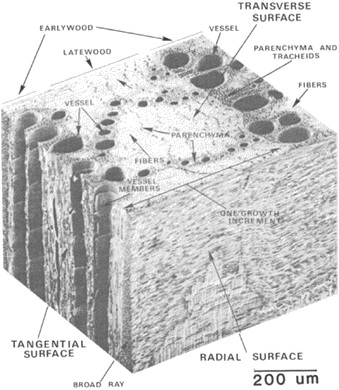
\includegraphics{Figures/Tracheids}
	\decoRule
	\caption[Wood microscopic composition]{Wood microscopic composition, presenting tracheids and vessels}
	\label{fig:Fig1}
\end{figure}
Tracheids allow to transport raw sap (from the ground, to the tree ramification) and elaborated sap (from the ramification to the ground). Some vessels are also perpendicular to wood grain. A phenomenon of capillarity explain how sap can circulate into vessels and tracheids. It is also explained by vegetative transpiration, due to photosynthesis and allow sap movement too \parencite{Reference1}.

Cambium has the role of cellular division \parencite{Reference4} presents it, in his document. Cambium will divide in two different cells. Phloem which is the component of the bark, and xylem which is the cell of sapwood.  All these cells are composed of polymers as cellulose, lignin, and hemicellulose. These cells by their configuration (as the crystal one) are as resistant as steal. Lignin has different interest, like the waterproofing on the cells’ walls. 
Wood is a material which has a specific behavior due to the change of the relative humidity of the middle. This behavior explains that norms forbid its utilization when its internal moisture content exceeds 20\%. Indeed, due to the microscopic properties, it appears that the tracheids expands with moisture content increase. Water present into tracheids and vessels, make it inflated which involve a displacement. On the contrary, when the temperature increase, and relative humidity decrease, tracheids contain less water and retract, but it also involves a displacement. This phenomenon known as Shrinkage - Swelling have an important effect because of the radial and tangential stresses which occurs when all the tracheids expands while the wood is displacement blocked. 
Each wood has a percentage of humidity called saturation fiber point (SFP) which is approximately 30\% amount of water. Under that point, free water contains in tracheids, and vessels will evaporate, and the water contain in cellulose fiber will begin to evaporate too. This effect involve withdrawal. At the opposite, if the amount of water increases and exceed 30\%, there is swelling. 
To provide these effects, wood is often treated and dry before uses. But drying a wood element can produce cracks. When the wood is dry too fast, a located collapse of cells and a crack takes place. The objective in the drying process is to limit the amount of water to nearly 12\%. At its initial state, green wood is considered as a wood full of water. To prevent water effect, and have a 12\% relative humidity inside it, a heating process must be done. Examples can be the stove or a constant ventilation. Indeed, a natural dry will take one year, while an artificial one like, blowing constant hot and humid (at least 70\% of humidity) air, will take one month. 
These information allow to understand the experiments which will be done in this thesis work. But before presenting the experiments, some theoretical knowledges must be reminded. 


%----------------------------------------------------------------------------------------
%	SUBSECTION 2
%----------------------------------------------------------------------------------------

\subsection{An anisotropic and orthotropic material}

Wood is considered as an orthotropic material because the behavior of its mechanical or thermal properties are not the same in its three mutually perpendicular directions. It is a particular anisotropy. This characteristic of the material can be explained by cellular arrangements, growth direction, and other biological elements \parencite{Reference1}. It involves mechanicals difference between each direction.
Wood has good mechanical characteristics. It is resistant in compression thanks to the strength of his structure. It is the same for traction resistance. However, this observation depend on the direction observed.  
The longitudinal direction presented on \ref{fig:Fig2}, is different from the others. Longitudinal direction is the one, which is the less impacted by water effects. Indeed, the tracheids swelling appears on the two others dimensions. So, it is a first independence of this direction on the others. Perpendicular plans, RL and RT are symmetrical. 
Therefore, regarding the tracheid constitution, it is trivial to understand that it is more resistant in terms of traction or compression. Tracheid are composed, \parencite{Reference4} of solid polymers like cellulose or lignin. However, in the others' direction, as tangential or radial one, a tracheid can be separated from the neighbor one, causing a crack due to the separation of tracheids. It is possible when the effort applied on the wood is a perpendicular (perpendicular from the longitudinal direction) traction one. That is why, tests are made on different surface.
\begin{figure}[th]
	\centering
	
\includegraphics{Figures/Wood Surfaces}
	\decoRule
	\caption[Wood surfaces]{Wood surfaces depending on the direction}
	\label{fig:Fig2}
\end{figure}
%----------------------------------------------------------------------------------------
%	SECTION 2
%----------------------------------------------------------------------------------------
\section{Wood species}

Wood are separated into different species and two different groups: the temperate species and tropical species. The literature shows that the tropical species have better resistance due to this more complex microscopic structure characterized by its growth’s environment. This work present experiment on both type of wood. It is important to notice that hardwood (wood from leave trees) and  softwood (wood from needles trees) have different behavior \parencite{Reference2}, but are presented in this work.

%----------------------------------------------------------------------------------------
%	SUBSECTION 1
%----------------------------------------------------------------------------------------

\subsection{Tropical species}

This work will focus on three tropical species, allowing to present woods with different density but from a same area, so dependent to same climatic constraints. Tropical types of woods are located in area, with an equatorial climate or humid tropical climate. Both are characterized by important rains. Equatorial climate has a constant and important pluviometry, while humid tropical climate is composed of a rainy season with torrential rains. Climate is one explanation of the growing differences between tropical and temperate species. In the case of this work, the study will be focused on three tropical species from Congo basin area (central Africa) in Gabon: Okume, Padouck and Iroko. All these species are heartwood ones. 

Okoume specie (Aucoumea klaineana), has the smallest density. It is a wood present in central Africa. The major advantage of this specie is the speed of growth, which is one of the most impressive in wood world. According to CIRAD data \parencite{Reference5}, it has a circumference between 60cm to 120cm and can reach 50m high. The color of this wood is composed of red nuances darkest depending on time. Rupture in compression occurs at a force of nearly 36\si{\mega\pascal} as \parencite{Reference5} present in Okoume wood sheet. It has a density of 0,44 which can be characterized as a light wood. It has a high SFP, equal to 40\% with a tangential withdrawal, superior to the radial one, and is in order of 6,9\%. For all this advantages, it is really used in construction, for carpentry, plywood, or shuttering panels. With a sapwood of approximately, 5\si{\centi\meter}, it allows to work with a large part of the three (heartwood principally). 

Padouck (Pterocarpus soyauxii Taub) is another tropical specie which has a bigger density, about 0,8 \parencite{Reference7}. It is considerate as a heavy wood. This characteristic explains its numerous uses in construction particularly. It can be used for bridge structure, carpentry, naval construction, plywood panels…   From 60\si{\centi\meter} to 100\si{\centi\meter} of diameter it also can reach 50\si{\meter} of high. It is less common and findable than Okoume specie. It must be dry, but it is an interesting wood in terms of natural durability class (heartwood is classed in first durability class)
The Padouck is also a red nuances wood. It is one of the better compression resistance wood in the world, with a resistance until 70\si{\mega\pascal}. It has a SFP around 21\% and a tangential withdrawal of 5\%.

Iroko (Milicia excelsa) is the last wood presented. It is a compromised between the precedent species. It is not a red wood, but a yellow, brown one. It has visible tracheids and a density around 0,65 \parencite{Reference7} . It is also used for many usages, but not particularly construction. It can be used for parquet, woodworking, or cover plywood panels. One of the major advantages of this wood is the transformation of CO2 into calcium oxide crystals. It also considered as a viable wood considering insect and fungus resistance. It has a compression limit equal to 54\si{\mega\pascal} and admit variation of 6\si{\mega\pascal} as mentioned by the CIRAD. It has a tangential withdrawal double from the radial one, this value is 5,4\% and the SFP is 23\%.


%----------------------------------------------------------------------------------------
%	SUBSECTION 2
%----------------------------------------------------------------------------------------

\subsection{Temperate woods}

These trees are located in temperate area and are impacted by temperate climate. It is known that the temperate climate is characterized by four seasons and two important ones, the spring and summer. Indeed, during autumn and winter, trees are not growing waiting for rain and sun, which are essential for its expansion. In spring, the tree needs a lot of water and the cambium produces a large amount of sapwood. This sapwood made in spring is softer and quickly done at the contrary of summer sapwood, heavier with a bigger density. This thesis will compare the three species presented before with a European specie, the Silver Fir. It is a softwood from needles tree. 

The Silver Fir (Abies pectinata). Present on north hemisphere, it is a softwood as Pines or others old trees. As his name undertone, it has a white color, and a circumference between 50 to 80cm. It has a density from 0,45 to 0.60 according to CIRAD data, a SFP about 30\% and a mechanical resistance in compression of 41MPa. The tangential withdrawal is important with a value of 8,7\%, while the radial withdrawal is 4\%. Thanks to it resistance, it is used in carpentry, columns or light frame but must be treated against fungus and insects’ attacks. The main problem with this wood is the water bag contained into the tree. It also has a problem of splitting which prevent uses of some connector in construction field.

%----------------------------------------------------------------------------------------
%	SECTION 3
%----------------------------------------------------------------------------------------
\section{Wood experimentation specimens}


%----------------------------------------------------------------------------------------
%	SUBSECTION 1
%----------------------------------------------------------------------------------------
\subsection{ Double Cantilever Beam (DCB) specimen}

%According to the different article on this test, it appears that it is used mainly with WS and DCB sample. As \parencite{Reference11} presents, it is a method permitting to study the crack tip and then estimate crack length during the wedge split test procedure. Most of the time, it is used in addition of DIC methods. For those reasons, this test is one of the most interesting in the presented case of a mode I study. It uses the compliance method for crack length estimation. 
%The test is simple, as it is visible on \ref{fig:Fig6} it consists of using two arms surrounding the specimen which is fixed to the press by metallic grips. The tested specimen must be adapted to the system, such as ARCAN one, proposed by \parencite{Reference6}. The efforts are applied by an electromechanical press, in this work, the MTS allow to obtain the force applied for a given displacement per second. The chosen grips are simpler than ARCAN ones and allow only mode one tests.
%\begin{figure}[th]
%	\centering
%	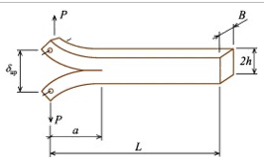
\includegraphics{Figures/DCB Test}
%	\decoRule
%	\caption[DCB Test]{Sheme of DCB Test in mode I, showing the different variables as $\delta_{ap}$, the opening length of the crack lips, a, the crack length, P the applied force and geometrical values of the specimen}
%	\label{fig:Fig6}
%\end{figure}
%A sensor detects the movements of the application point of the forces.
%Therefore, a camera is placed in the axis of the crack in order to use the images and study the crack.

DCB specimens are mainly used in opening mode. The geometry is simple, often rectangular, it has one dimension longer than the two other. The crack propagate in this more important dimension, allowing a displacement of the fracture process zone as presented in \ref{fig:DCB}.
\begin{figure}[h]
	\centering
	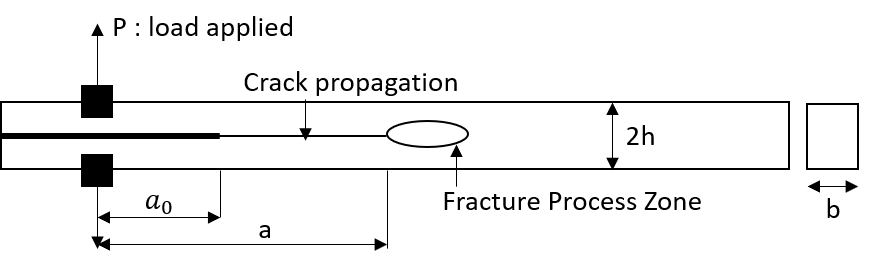
\includegraphics{Figures/DCB}
	\decoRule
	\caption[DCB specimen]{DCB specimen tested by application of a load P}
	\label{fig:DCB}
\end{figure}
The tests on these samples allow the determination of the energy release rate in mode I, which is the parameter that we want to compare. The DCB test specimens permits also to obtain the stress intensity factor.
These specimens are interesting thanks to this important range of propagation of the crack. The compliance method is used on these specimens because of the CTOD, which is easily calculated. Indeed, it is similar to study two pieces of wood and measured the distance between each. This distance is the crack tip opening displacement, depending on time. However, the crack can be unstable if the material is heterogeneous, which is the case with wood, for instance when a knot is present. In order to avoid these instabilities, \parencite{Reference10} proposed a DCB specimen with variable inertia.
This variable geometry, although not allowing the study of mode II obtains a better stability and an easier study of the propagation of crack.

%----------------------------------------------------------------------------------------
%	SUBSECTION 2
%----------------------------------------------------------------------------------------
\subsection{ Compact Tension Shear (CTS) specimen}

Many scientists have worked with an alternative geometry, the Compact Tension Shear specimen. Mainly used on metallic or resinous materials, it can also be used on materials such as wood. The test is simple, as it is visible on \ref{fig:CTS} it consists of using two steel arms surrounding the specimen which is fixed to the press by metallic grips. The tested specimen must be adapted to the system, such as ARCAN one, proposed by \parencite{Reference6}. Indeed, stress holes where are applied opposite forces as shown on \ref{fig:CTS} allow to obtain a crack propagation generally propagating in the RL surface. To proceed in mixed mode, the forces have to be applied with an angle. 
\begin{figure}[h]
	\centering
	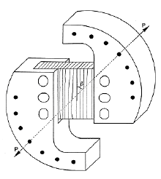
\includegraphics{Figures/Specimen_test}
	\decoRule
	\caption[CTS specimen]{CTS specimen tested in mode III by angular loads}
	\label{fig:CTS}
\end{figure}
One interest of this type of sample is that this test is possible in crack opening mode, but also in shear mode or in mixed mode. Another  advantage is linked to these dimensions, smaller than those of DCB for instance. This is an interesting point for this work to reduce the volume which must be submerged to gain in MC.

%----------------------------------------------------------------------------------------
%	SUBSECTION 3
%----------------------------------------------------------------------------------------
\subsection{ Mixed Mode Crack Growth (MMCG) specimen}

So many geometries can be used to allow experimental studies. This thesis, inspired on previous work use MMCG specimen which derivate from DCB and CTS specimen presented before. The purpose of MMCG specimen, \parencite{Reference6} is to involve a stable propagation of the crack in different mode and in mixed mode too. The study of this sample uses the rate of refund (G). G decrease while the crack is developing, until sample rupture. Tests on MMCG specimen can be study thanks to finite elements like the J integral method, which is used in this work. But also, by image analysis, like the DIC analysis.
\begin{figure}[th]
	\centering
	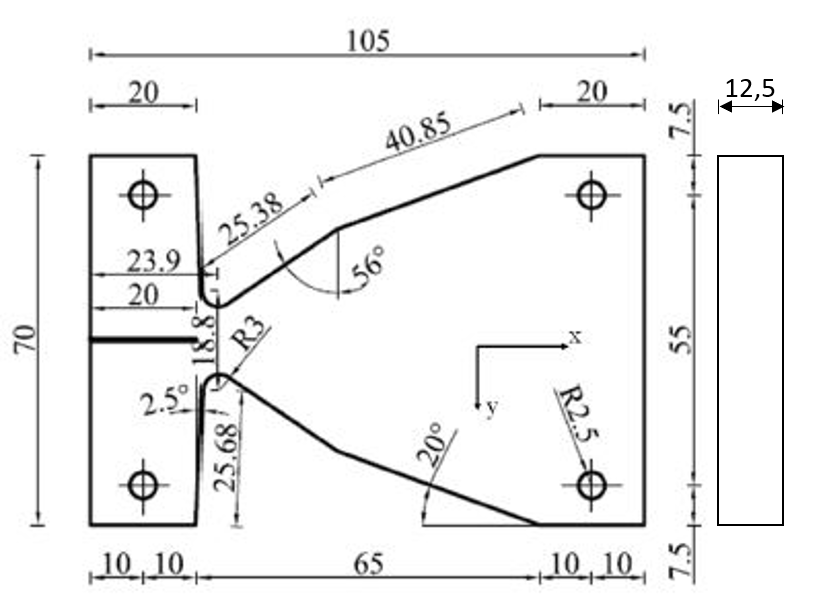
\includegraphics[scale=0.5]{Figures/MMCG_specimen}
	\decoRule
	\caption[MMCG specimen]{dimensions and geometry of Mixed Mode Crack Growth specimen}
	\label{fig:Fig5}
\end{figure}
MMCG sample is a compromise between DCB and CTS samples to obtain different mixing rates and a stable crack propagation. It is the specimen which will be used for this Development and Research Project, because of the good stability of the sample, presented in \parencite{Reference6} thesis. The Geometry, visible on \ref{fig:Fig5} was already tested in \parencite{Reference7} works. Manufactured samples of Okoume species with these dimensions were available in Polytech laboratory.

MMCG shapes are linked to Compact Tension Shear (CTS) specimen due to the tiny dimensions of MMCG samples which are similar to CTS ones. This geometry involves a little Fracture Process Zone (PFZ) which begin at the crack tip. But at the contrary of DCB specimen, the smaller dimensions of MMCG specimen does not allow a long displacement of the PFZ during the test. So after few minutes of displacement of the crack tip, the specimen will break. It is linked to DCB specimen because of \parencite{Reference10} work and the creation of variable inertia in DCB specimens. It must be noted, that the chosen MMCG specimen are RL samples so with a Radial and Longitudinal surface. The Tangential direction corresponds to the thickness of specimens. It means that the  swelling principally involves an expansion of the specimen thickness.

In mode one, a really progressive crack is expected. As it was said, \parencite{Reference6} developed this particular shape, to improve the stable propagation of the crack, more than in a DCB sample. Moreover, the different angles shown on \ref{fig:Fig5} and the rounded chamfer provide uncontrollable collapse of the specimen. Indeed, the optimization consists, on the variable inertia also used in DCB specimens. It was proved by Finite Element Analysis (FEA) that the connection between the heels and the body of the specimen is a zone where strains are concentrated. These shapes, allow by limiting the surface, to avoid wood heterogeneity. Besides, this compact geometry involves a faster increase of the MC in the specimen. It is logical but can be reminded by \ref{eq:moisture flux in wood}

\begin{equation}
\begin{array}{l}
	q_{m}= -\rho_{0}\cdot D \cdot \bigtriangledown m 
	\\
	\\
	\left\{
	\begin{array}{lll}
	q_{m}: & $moisture flux$ & \si{\square\meter\per\second} \\
	D: & $Diffusivity$ & \si{\square\meter\per\second} \\
	\bigtriangledown: & $Gradient$ & . \\ 
	m: & $moisture content$ & \% \\
	\end{array}{}
	\right.
\end{array}{}
	\label{eq:moisture flux in wood}
\end{equation} 


%----------------------------------------------------------------------------------------
%	SUBSECTION 4
%----------------------------------------------------------------------------------------
\subsection{ Climatic effects on the test }

This work studies the impact of temperature and moisture content variation on wood samples. The moisture content have an impact on the studied parameters as the energy rate or the mechanical resistance. Moreover, it is a phenomenon, present in the wild, which participate to wood life. Non precise technics allow to have an idea of the moisture content in the wood. But every specie is different and even, each tree is different. 
Without moisture meter, the moisture content in our specimens is determined by the weight measurement of the sample. The concept is to dry the specimen to obtain the anhydrous weight. Thanks to this measure ($M_{0}$), and the actual weight ($M_{S}$) the \ref{eq:Moisture content depending on weight} is :
\begin{equation}
	H=\frac{_{M_{S}-M_{0}}}{M_{0}}100
	\label{eq:Moisture content depending on weight}
\end{equation} 

The species presented were chosen among many others for different reasons. First, they have an interesting and different behavior. Indeed, they have different density but also mechanical behavior and are from different area and type of woods, as explained before. Then, there are really linked to the Civil engineering subject. Except Okoume specie, all the other are not enough exploited for construction uses. Gabon forest are composed of many wood, but without the use of some of them in construction field, as for Iroko and Padouck species. In France, the same fact appears in Massif Central forest, composed of many Silver Fir areas. By proving that these species have a good behavior in humid environment, it could allow, their use in Construction field. Looking to \parencite{Kif1998}, \parencite{Ang2017}, \parencite{Huang2020} works presenting wood behavior at different moisture content, or \parencite{Seif2017} for severals temperature, some values can be expected. Indeed, it is not the first work on this subject and our results could be discussed according to other articles.

Indeed, researches were also, already done on the subject, like \parencite{Reference12} studied on Jack pine (Pinus banksiana) and balsam poplar. He observes the mechanical properties of wood, function of the moisture content and temperature. It appears that another possibility to modify the moisture content, is the use of solution. \parencite{Reference12} presents three principal solutions, placed in a desiccator: MgCl2, NaNO3 and KCl. 

Another climatic condition, which must be considered, is the temperature. The temperature can involve an augmentation of moisture content. Tests are done on this sample at normal temperature, but also at a lower one by putting specimen during 48 hours into a fridge. This experiment allows to prove the gain of moisture content due to the decreasing temperature. Scientists as \parencite{Reference13} did tests on sample under different temperature, 20\textcelsius, 40\textcelsius, 60\textcelsius and 80\textcelsius but also 100\textcelsius to 200\textcelsius during two hours for some DCB samples.
Tested samples were DCB ones and the species were Spruce and Beech. Results from works as \parencite{Reference12} on Balsam Poplar, but with compressive tests in a radial direction, allow to have an idea of the way to proceed and the attempt results. 

\begin{table}[h]
	\centering
	\begin{tabular}{cccc}
		\hline
		\rowcolor[HTML]{BFBFBF} 
		\multicolumn{1}{c}{\cellcolor[HTML]{BFBFBF}Reference} & \multicolumn{1}{c}{\cellcolor[HTML]{BFBFBF}Specie} & \multicolumn{1}{c}{\cellcolor[HTML]{BFBFBF}Climatic Variation} & \multicolumn{1}{c}{\cellcolor[HTML]{BFBFBF}Result} \\
		\multicolumn{1}{c}{\cellcolor[HTML]{FFE699}\cite{Kif1998}} & \multicolumn{1}{c}{Scots Pine} & \multicolumn{1}{c}{Earlywood Green} & \multicolumn{1}{c}{$\sigma$ = 49MPa} \\
		\multicolumn{1}{c}{\cellcolor[HTML]{FFE699}\cite{Kif1998}} & \multicolumn{1}{c}{Scots Pine} & \multicolumn{1}{c}{Latewood Green} & \multicolumn{1}{c}{$\sigma$ = 74MPa} \\
		\multicolumn{1}{c}{\cellcolor[HTML]{FFE699}\cite{Kif1998}} & \multicolumn{1}{c}{Scots Pine} & \multicolumn{1}{c}{Earlywood resoaked} & \multicolumn{1}{c}{$\sigma$ = 36MPa} \\
		\multicolumn{1}{c}{\cellcolor[HTML]{FFE699}\cite{Kif1998}} & \multicolumn{1}{c}{Scots Pine} & \multicolumn{1}{c}{Latewood resoaked} & \multicolumn{1}{c}{$\sigma$ = 55MPa} \\
		\multicolumn{1}{c}{\cellcolor[HTML]{B4C6E7}\parencite{Ang2017}} & \multicolumn{1}{c}{Douglas Fir} & \multicolumn{1}{c}{9\% MC} & \multicolumn{1}{c}{$G_{max}$= 780J/$m^{2}$} \\
		\multicolumn{1}{c}{\cellcolor[HTML]{B4C6E7}\cite{Ang2017}} & \multicolumn{1}{c}{Douglas Fir} & \multicolumn{1}{c}{18\%MC} & \multicolumn{1}{c}{$G_{max}$= 680J/$m^{2}$} \\
		\multicolumn{1}{c}{\cellcolor[HTML]{B4C6E7}\cite{Ang2017}} & \multicolumn{1}{c}{White Fir} & \multicolumn{1}{c}{9\% MC} & \multicolumn{1}{c}{$G_{max}$= 580J/$m^{2}$} \\
		\multicolumn{1}{c}{\cellcolor[HTML]{B4C6E7}\cite{Ang2017}} & \multicolumn{1}{c}{White Fir} & \multicolumn{1}{c}{18\%MC} & \multicolumn{1}{c}{$G_{max}$= 630J/$m^{2}$} \\
		\multicolumn{1}{c}{\cellcolor[HTML]{C6E0B4}\cite{Huang2020}} & \multicolumn{1}{c}{Jack Pine} & \multicolumn{1}{c}{2\% MC} & \multicolumn{1}{c}{$\sigma$ = 4,5MPa} \\
		\multicolumn{1}{c}{\cellcolor[HTML]{C6E0B4}\cite{Huang2020}} & \multicolumn{1}{c}{Jack Pine} & \multicolumn{1}{c}{17\% MC} & \multicolumn{1}{c}{$\sigma$ = 2,9MPa} \\
		\multicolumn{1}{c}{\cellcolor[HTML]{C6E0B4}\cite{Huang2020}} & \multicolumn{1}{c}{Balsam Poplar} & \multicolumn{1}{c}{2\% MC} & \multicolumn{1}{c}{$\sigma$ = 5,4MPa} \\
		\multicolumn{1}{c}{\cellcolor[HTML]{C6E0B4}\cite{Huang2020}} & \multicolumn{1}{c}{Balsam Poplar} & \multicolumn{1}{c}{17\% MC} & \multicolumn{1}{c}{$\sigma$ = 3,7MPa} \\
		\multicolumn{1}{c}{\cellcolor[HTML]{F4B084}\cite{Seif2017}} & \multicolumn{1}{c}{Numerical} & \multicolumn{1}{c}{-10 °C} & \multicolumn{1}{c}{G = 8J/$m^{2}$} \\
		\multicolumn{1}{c}{\cellcolor[HTML]{F4B084}\cite{Seif2017}} & \multicolumn{1}{c}{Numerical} & \multicolumn{1}{c}{0 °C} & \multicolumn{1}{c}{G = 9J/$m^{2}$} \\
		\multicolumn{1}{c}{\cellcolor[HTML]{F4B084}\cite{Seif2017}} & \multicolumn{1}{c}{Numerical} & \multicolumn{1}{c}{10 °C} & \multicolumn{1}{c}{G = 11J/$m^{2}$} \\
	\end{tabular}
	\caption{Approximative results from previous works on climatic conditions affecting wood behavior.}
	\label{tab:ArticleResult}
\end{table}

The last climatic conditions, presented is the fatigue load. Even if it is not a real climatic effect, it could be involved by the climate like a snow load. This is the last experiment which will be done on the specimen. Fatigue is directed by Paris law, as the \ref{eq:Paris law, fatigue loads equation} :
\begin{equation}
	\frac{\partial a}{\partial N}=C \Delta K^{m}
	\label{eq:Paris law, fatigue loads equation}
\end{equation} 
With “a”, the crack length, “N” the number of loading cycles, which involve that $\frac{\partial a}{\partial N}$ is the crack growth rate. It depends on the cyclic stress intensity factor $\Delta K$. Finally, “C” and “m” are empirical constants depending on the studied material, but also the frequency, the load ratio, the temperature... This equation allows anticipating crack growth rate and predict fatigue comportment of the material.  

So it is expected that with an increase of the moisture content, the mechanical behavior must decrease, while by increasing the temperature of the specimen, the mechanical behavior should increase, as it is visible in \ref{tab:ArticleResult}. However, this fact will also depend on the specie study.
Linked to the Moisture Content, if the temperature increase, there are less MC into the specimen, so it is expected that with a higher temperature, wood behavior should be better.

%----------------------------------------------------------------------------------------
%	SECTION 4
%----------------------------------------------------------------------------------------
\section{Wood fracture mechanics}


%----------------------------------------------------------------------------------------
%	SUBSECTION 1
%----------------------------------------------------------------------------------------
\subsection{Fracture modes and process zones}

Fracture mechanic has an objective to characterize the cracking behavior of structures through stress field, crack size and cracking resistance of the material.

There are different rupture modes involve by the crack, the direction of the force which create the crack or compounds it. The first mode, called opening mode, characterized by a force applied, perpendicularly to the crack. The shearing mode is the second mode. The force is applied parallelly to the crack. And the third mode of rupture parallelly to the interior of the crack. The principals rupture mode are the first and the second, and this literature review will focus on first mode particularly. These modes are presented on \ref{fig:Fig3}. This first mode can be presenting by the energy release rate (G) linked to time or in our case, crack length, this plot is called R-curve.
\begin{figure}[th]
	\centering
	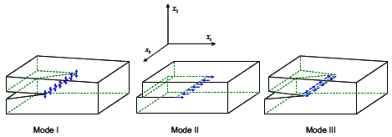
\includegraphics{Figures/Mode_presentation}
	\decoRule
	\caption[Crack modes]{Crack modes depending on the direction of the applied force.}
	\label{fig:Fig3}
\end{figure}
Four zones characterized this propagation crack. The first is a stationary phase, with an increase of G until a critical value in mode 1, “$G_{IC}$” reached at a critical time, called tc. Then a second phase correspond to the crack propagation and occurs at a constant value of G. In the third zone, G decrease and the crack propagation stop. At least, the fourth phase involve material ruin shown by G fast increase, which correspond to an instability.

There are different types of cracks. The crack depends on the microscopic structure of the material, the loading conditions, and many other factors.

Rupture by brutal cracking : it happens on materials with a very high resistance, the working stresses are very high. The presence of small cracks can cause this sudden rupture without plastic deformation. 
Rupture by successive growth of cracks : Also called fatigue failure. The mechanical factors that influence this phenomenon is displacements, strains, and stresses, but also environmental conditions such as temperature or relative humidity. It is easier to observe because it takes more time to involve samples destruction than a unique and sudden crack. Indeed, it is a succession of small cracks from an initial crack. In experimental works, it is often created by a circular saw and the last millimeters of the initial crack, are made by a cutter.  

The test done is filmed to determinate how the cracks will be developed over time, depending on the applied forces. With a material like wood, successive cracks rupture are expected. It is important to notice that different zones are studied. There are three areas. 

First one is the development zone: It is the closest zone to the crack. The study is difficult due to the high stresses which cause irreversible damage to the material. The stress field into the crack is maximal. Indeed, the constraints are modelled, as explained with the equation \ref{eq:stress term σ_11} :
\begin{equation}
	\left\{
	\begin{array}{rcr}
		\sigma_{11}=\frac{K_{1}}{(\sqrt{2 \pi r})}Re[\frac{s_{1}s_{2}}{(s_{1}-s_{2})}(\frac{s_{2}^{2}}{\sqrt{\rho_{2}}}-\frac{s_{1}}{\sqrt{\rho_{2}}})]+\frac{K_{2}}{(\sqrt{2 \pi r})}Re[\frac{1}{(s_{1}-s_{2})}(\frac{s_{2}^{2}}{\sqrt{\rho_{2}}}-\frac{s_{1}}{\sqrt{\rho_{1}}})]	
	\end{array}
	\right.
	\label{eq:stress term σ_11}
\end{equation} 

So, if the study is close to the bottom crack, the “r” factor will decrease, and the constraints will approach to infinite values.

\begin{figure}[th]
	\centering
	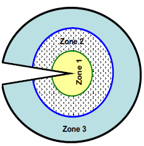
\includegraphics{Figures/Crack_zones}
	\decoRule
	\caption[Crack zones]{Names of each part of the crack}
	\label{fig:Fig4}
\end{figure}

The second zone, visible on \ref{fig:Fig4} is called singular zone: it circled the first zone. The mechanical field does not depend on specimen geometry. Interface between zone one and two, has continuous constraints and displacements values.

The last zone is the farthest zone from the crack tip. It is the zone which is in contact with loads and displacements forces.

%----------------------------------------------------------------------------------------
%	SUBSECTION 2
%----------------------------------------------------------------------------------------
\subsection{Mechanical fields}
There are 2 mechanical fields, isotropic and orthotropic fields. Because of wood behavior, the orthotropic mechanical filed will be the only one presented. 
The elastic stress field, near the crack tip, depends on the material. For an orthotropic material, the expression, presented in \parencite{Reference10} work are :

\begin{equation}
	\left\{
	\begin{array}{rcr}
		\sigma_{11}=\frac{K_{1}}{(\sqrt{2 \pi r})}Re[\frac{s_{1}s_{2}}{(s_{1}-s_{2})}(\frac{s_{2}}{\sqrt{\rho_{2}}}-\frac{s_{1}}{\sqrt{\rho_{2}}})]+\frac{K_{2}}{(\sqrt{2 \pi r})}Re[\frac{1}{(s_{1}-s_{2})}(\frac{s_{2}^{2}}{\sqrt{\rho_{2}}}-\frac{s_{1}^{2}}{\sqrt{\rho_{1}}})]\\
		\sigma_{22}=\frac{K_{1}}{(\sqrt{2 \pi r})}Re[\frac{1}{s_{1}-s_{2}}(\frac{s_{1}}{\sqrt{\rho_{2}}}-\frac{s_{2}}{\sqrt{\rho_{1}}})]+\frac{K_{2}}{(\sqrt{2 \pi r})}Re[\frac{1}{(s_{1}-s_{2})}(\frac{1}{\sqrt{\rho_{2}}}-\frac{s_{1}}{\sqrt{\rho_{1}}})]\\
		\sigma_{21}=\sigma_{12}=\frac{K_{1}}{(\sqrt{2 \pi r})}Re[\frac{s_{1}s_{2}}{(s_{1}-s_{2}}(\frac{s_{1}}{\sqrt{\rho_{1}}}-\frac{1}{\sqrt{\rho_{2}}})]+\frac{K_{2}}{(\sqrt{ 2\pi r})}Re[\frac{1}{(s_{1}-s_{2})}(\frac{s_{1}}{\sqrt{\rho_{2}}}-\frac{s_{2}}{\sqrt{\rho_{1}}})] \\
	\end{array}
	\right.			
	\label{eq:stresses terms from Orthotropic field}
\end{equation} 

In these equations presented in \ref{eq:stresses terms from Orthotropic field}, $S_{i}$ with i = {1;2} are the polynomial roots calculated by another equation, using the components of the stiffness tensor for an orthotropic symmetry. 
Therefore, terms
\begin{equation}	
	\rho_{j}=\cos{\theta}+i s_{j} \sin{\theta} and j\in{[1;2]}
	\label{eq:terms present in stress equations}
\end{equation}			
These theories, are already used, and the orthotropic equations will be those that will be used for wood experiments. Indeed, even if the resolution could be done by ourselves, there are nowadays, computer software, which allow us to spend less time resolving orthotropic equations. It is written in the software program, and run, until finding solutions.

%----------------------------------------------------------------------------------------
%	SUBSECTION 3
%----------------------------------------------------------------------------------------
\subsection{Stress Intensity Factor}
K is  the stress intensity factor, and $K_{Ic}$, is the one for the opening mode. The "c" means that it is the critical value of this coefficient. As \parencite{Reference10} explains, by using Laplace Carson inverse on Stress Intensity Factor (SIF), it is possible to obtain crack opening factors. Focusing on mode I, it is particularly interesting to understand how $K_{Ic}$ evolves. The stress intensity factor K can be obtained by using finite element analysis (for example, with a contour integral method for orthotropic materials). It is obtained with the initial crack length $a_{initial}$ linked to the crack length L : $\frac{a_{initial}}{L}$.
The stress intensity factor depends on the specimen geometry. The classic linear elastic fracture mechanics equation for SIF is presented in \ref{eq:Intensity factor}:
\begin{equation}
	K_{I}=\frac{P}{W\sqrt{L}}f\frac{a_{initial}}{L} 	
	\label{eq:Intensity factor}
\end{equation} 						
P : the force applied on the specimen 
W the thickness
L the crack length 
f the linear function which link the terms $a_{initial}$ and L in $\frac{a_{initial}}{L}$. 

It also associated to the Stress Intensity Factor (SIF) name. 

%----------------------------------------------------------------------------------------
%	SUBSECTION 4
%----------------------------------------------------------------------------------------

\section{Energetic methods}

Different methods were created to work on fracture mechanics, called energetic methods. $G_{\theta}$ or $M_{\theta}$ which are defined on surface contours. J and $G_{\theta}$ are useful for pure shearing or opening tests, due to a global energetic operation. All the presented integral with a $\theta$ terms have an important difference. They are defined on a surface contour, which is easier to integrate. M-integral has two terms, depending on real or virtual displacements involving real and virtual constraints, which allow decoupling modes
A-integral is an independent integral which allows to consider the effect of thermo-hygro-mechanical loads in the cracking process. During the crack process, it uses temperatures data. As T-integral, it is similar to M-integral, and do not include the crack tip, which is a particular part of the crack (too many singularities).

In this work, the chosen method, which is created in a Python program to carry out this work is the Rice Integral.

Rice Integral is presented as the next formula \ref{eq:J, Rice integral} :
\begin{equation}
	J=\int_{\Gamma}[F n_{1}-\sigma_{ij} n_{j} \frac{\delta u_{i}}{\delta x_{1}}]d\Gamma
	\label{eq:J, Rice integral}
\end{equation}  

The considered contour of this integral is curvilinear and is named $\Gamma$. It includes the crack tip while it is not the case of others energetic method. “F” is the force applied on each part of the crack tip. Then, “a” is still the length of the crack. “$n_i$“ are the normal vectors to the curvilinear contour $\Gamma_{i}$, and $\sigma$ is the strain used to obtain crack opening. 
There are better energetics methods. As $G_{\theta}$ or $M_{\theta}$ which are defined on surface contours. J and $G_{\theta}$ are useful for pure shearing opening, due to a global energetic operation. But J integral also allows to work on mode I cases. Then we will also use the compliance method to obtain the energy release rate.

%----------------------------------------------------------------------------------------
%	SUBSECTION 4
%----------------------------------------------------------------------------------------

\section{Compliance method}

Compliance is the characterizing quantity of material elasticity behavior. An elasticity compliance corresponds to the inverse of material elastic modulus. Its unity is the $Pa^-1$.
Compliance method is used to determinate the crack resistance. 
The formula used to calculate this energy release rate is written on \ref{eq:Energy release rate equation}:
\begin{equation}
	G_{c}= \frac{F_{c}^2}{2b} (\frac{\Delta C}{\Delta a})_{d} 	
	\label{eq:Energy release rate equation}
\end{equation}  
With : 
$G_c$ the value of energy release rate (in \si{\joule\per\square\meter})
$F_c$ the critical force which involves the crack (in \si{\newton})
b the thickness of the specimen (in \si{\milli\meter})
$\Delta C$ the compliance evolution (in $Pa^-1$)
$\Delta a$ the crack length evolution (in \si{\milli\meter})
In this work, C is determined in forced displacement, by the division of U, which is the imposed displacement, by F, the applied force. It must be noted that to have an idea of the imposed displacement depending on time, some articles as \parencite{Reference7} or \parencite{reference15} allow to fix this displacement between 2\si{\milli\meter\per\minute} until 5\si{\milli\meter\per\minute}.

As explained in previous part, the specimen presenting a RL surface studied have a Tangential dimension for their thickness. It involves a dimension evolution of this parameter. So for each test at a different MC, the b parameter must be measured, in order to have a precise value of G. Compliance method is often used in mode I analysis. It was the way of study for works as \parencite{Reference7}, \parencite{Ang2017}...

%----------------------------------------------------------------------------------------
%	SECTION 5
%----------------------------------------------------------------------------------------
\section{Software programms and analyzing tools}

%----------------------------------------------------------------------------------------
%	SUBSECTION 1
%----------------------------------------------------------------------------------------
\subsection{Image Correlation knowledges}

Image analysis is a powerful tool. Indeed, the number of domains using it is numerous. Everybody has already seen the facial recognition system working. It is similar to the fracture mechanic uses. It works by comparing two images, a first one putted in the system, and another when a person wants to unlock the system. If the two images are similar with a percentage of error, it will work.
The first use was for fluid mechanic. It was the first field which used image analysis. Indeed, it was easier with old camera to follow a moving point into fluid, than a point into a solid, because the displacement is smaller and difficult to observe if the resolution is not good enough.
Agronomic field is concerned too. Fernando Mendoza work explain how image analysis is used to determinate apples properties. Indeed, by analyzing apple images, he can determinate the optimal day for the harvest. He looks at special characteristics, like firmness and soluble solids content to obtain the best apple for consumers.

To focus on the one used in this work, digital measurement techniques using pictures, is a really interesting tool to work on fracture mechanics. Digital Image Correlation (DIC) consists in comparing two images of the same object on load, as MMCG specimen in our case, and looking to the displacement field, in order to find a match between the two images. When a series of images is obtained, the comparison between these images, and their differences are analyzed very accurately, pixel by pixel to obtain the real displacements, from one point to another place. The main problem of this technique is due to “noise” which involve uncertainties. Therefore, light problems can occur and decrease the precision of the results. In this method it is necessary to extract the two images (before and after movement).

The DIC method is based on the principles of mechanical continuity (rigid body mechanics). The system consists of using a digital camera and specialized computer software, in this work, MatchID. Camera is used to capture consecutive images of the tested sample surface during the deformation test. Digital images determined by this way, which corresponds to a series of photos, is analyzed by the DIC software. Displacement maps of specimen on the surface is created. Stress fields can be evaluated from strain fields. The formula used to obtain the displacement field is shown in \ref{eq:displacement field obtained by DIC methods}

\begin{equation}
	u^{k}=
	\begin{bmatrix}
		u_{z}^{k}\\u_{y}^{k}
	\end{bmatrix}
	=\Sigma^{N}_{i=1}
	\begin{bmatrix}
		f_{i}(k,\phi_{k}) & g_{i}(k,\phi_{k})\\ l_{i}(k,\phi_{k}) & m_{i}(k,\phi_{k})
	\end{bmatrix}
	\begin{bmatrix}
		A^{i}_{1}\\A^{i}_{2}
	\end{bmatrix}
	\begin{bmatrix}
		r^{i/2}_{k}
	\end{bmatrix}
	+
	\begin{bmatrix}
		T_{x}\\T_{y}
	\end{bmatrix}
	+
	R
	\begin{bmatrix}
		y_{k}\\y_{k}
	\end{bmatrix}
	\label{eq:displacement field obtained by DIC methods}
\end{equation} 

With $f_{i}$, $g_{i}$, $l_{i}$, $m_{i}$, polar functions, k is depending on the material because of Poisson term which determinates k. T terms are correction factors for rigid body motions.
Due to the fast and easy preparation, it is a very used fracture mechanic technique. After the determination of the displacement field, by using the integral method presented in last sections, it is possible to obtain the strain field.

If this method is used on wood, it is important to note that elastic orthotropic material model in 2D has five engineering constants as input parameters, to enter in the image analysis system. Even if it depends on the software used, these inputs are important to be known. First, Young modulus in longitudinal direction must be informed, $E_{L}$=$E_{1}$, transverse Young modulus $E_{trans}=E_{R}=E_{T}=E_{2}$. Then, shear modulus $G_{LR}=G_{LT}=G_{12}$, if shearing mode is studied. Therefore, Poisson coefficient $\nu$ has to be put into the software. This coefficient can change depending on the studied surface, in or out the plan. The initial crack length is introduced in the model. The damage description is presented by three principal inputs, even if it could change, depending on the software. Focusing on mode I damage, it is described by damage initiation stress $\sigma_{ini}$, but also separation at the failure $\delta_{fl}$, and exponential function shape coefficient $\alpha_{I}$. 

Beside, other technics could allow to do the same analysis. The only changement is linked to the pattern put on the specimen to follow the displacement and deduct the strain field. It could be a grid as in \parencite{Reference7} work or a marker.

%----------------------------------------------------------------------------------------
%	SUBSECTION 2
%----------------------------------------------------------------------------------------
\subsection{Analysis Software}

One of this work purpose, was to compare experimental wood behavior and analytic one.
Numerical simulation is a representation of complex physical phenomena. This is a way to virtually simulate a product in its final environment or submitted to different stress. In this work case, the fracture propagation was the physical phenomenon which have to be simulated. To do this job, many software tools were available. SolidWorks was a great candidate. Indeed, it is easy to use it and find tutorial to quickly learn. A try was done as visible on \ref{fig:SolidWorks}. As presented in \parencite{Reference8} and visible on \ref{fig:SolidWorks} thesis three areas are more impacted than the others. It must be noted, that before creating Okoume material on SolidWorks, steel was applied on this MMCG shape, in order to have a look on the behavior. By imposing 20\si{\milli\meter} of displacement, the specimen collapse, occurs in the holes' area. In the current example, a force is applied on the heel to avoid the bending moment which occurs on the upper heel. Indeed, by the application of the load in the upper hole, this part of the specimen is bending. The heel load is like a boundary condition as the one applied in the other hole. The \ref{fig:SolidWorks} example is an Okoume specimen with a 1\si{\centi\meter} notch. A static test is done by the traction from one hole at a load of 400\si{\newton}. This load is higher than the values given by \parencite{Reference7} thesis but allow to obtain values. So even if SolidWork is not as complete as others, this software permit the highlight of constraints areas. Indeed it is not possible to follow a crack evolution or really use the temperature or humidity coefficient to impact an experiment.

So the chosen software was Abaqus.
Indeed, to proceed a non-linear and multi-physics experiment, as with an orthotropic material submitted to climatic condition changes, Abaqus seems to be the best software. It allows to work on complex materials. Indeed, Abaqus makes possible to set up very complex and personalized material behaviors, including the definition of failure criteria. The user can use metallic, hyper-elastic, plastic or even composite materials. In addition, the material properties can also vary depending on field variables such as temperature.

Abaqus, also allows working on non linearity problem. Indeed, the contact resolution algorithm is very powerful. It takes into account very complex contact behaviors which consider large rotations and friction.  It is possible to work on static and dynamic problems, in 2D or 3D.
On this software, it is possible to create shape of the part on other application as CATIA or SolidWorks. Indeed, associative interfaces allow the transfer of geometry from a CAD system to Abaqus.

It works as a Finite Element Method solver. The procedure is user-friendly. First, it is necessary to create the shapes of the specimen which will be tested experimentally, in this case a MMCG specimen. This creation system is not as intuitive as the others steps. But by importing the shapes from another software, it can make the task easier. Then the different stages are presented by the interface as on \ref{fig:Abaqus_interface}.
\begin{figure}[th]
\centering
\begin{subfigure}{0.48\linewidth}
\centering
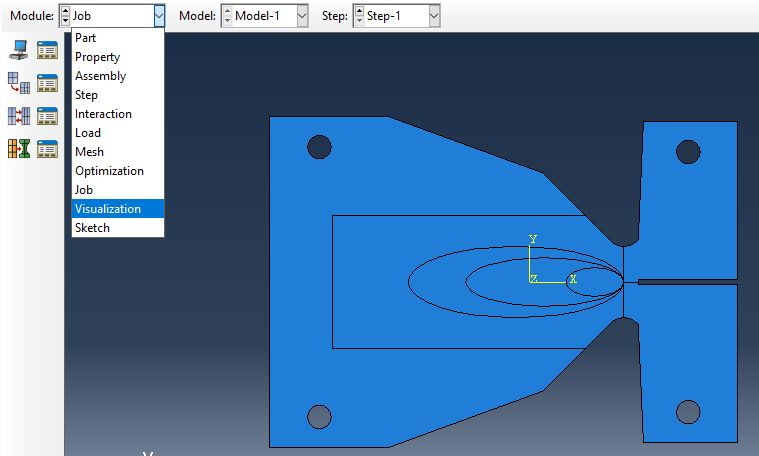
\includegraphics[scale=0.5]{Figures/Abaqus_fct}
\decoRule
\caption[Abaqus interface]{Different stages for Abaqus creation model presented next to a MMCG specimen part}
\label{fig:Abaqus_interface}
\end{subfigure}
\\
\begin{subfigure}{0.48\linewidth}
\centering
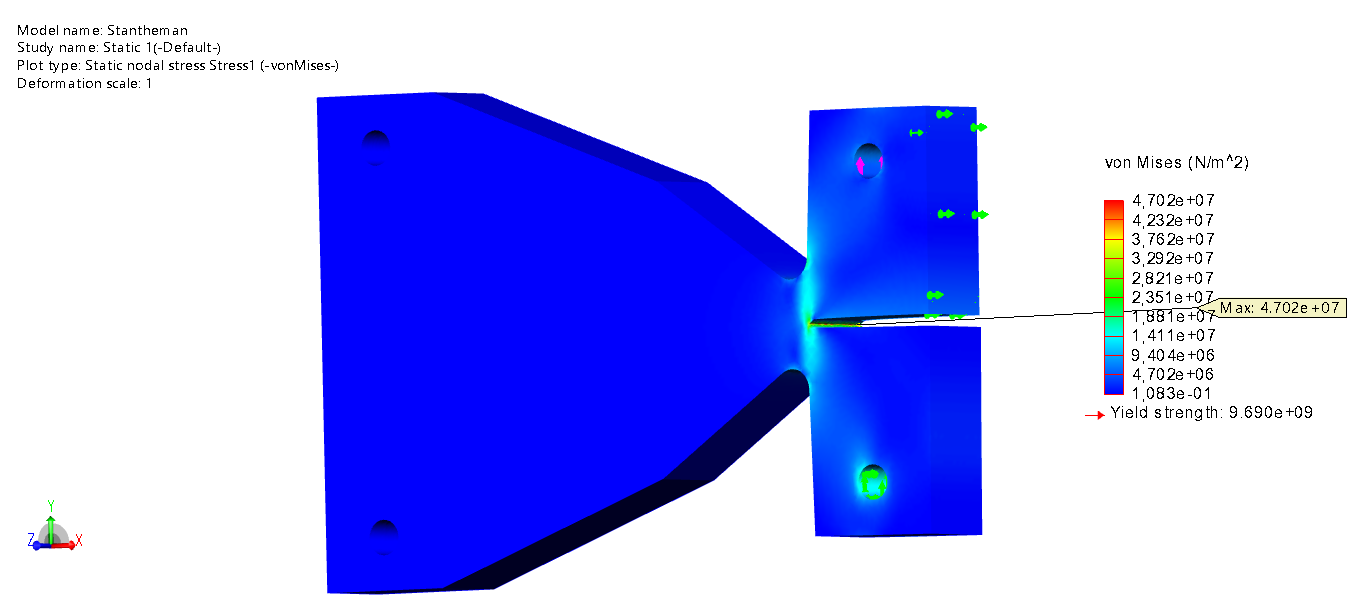
\includegraphics[scale=0.35]{Figures/SolidWorks}
\decoRule
\caption[SolidWorks analysis of Okoume specimen]{Example of SolidWorks analysis on Okoume specimen loaded }
\label{fig:SolidWorks}
\end{subfigure}
\caption[Software analysis]{Software analysis}
\label{fig:Softwares}
\end{figure}
So after creating the shapes, a material must be added to the part. By creating an entire material, the true values of Okoume, PAdouck and Iroko can be associated to the shapes. Then, some interaction must be input, as the force applied on the part or the boundariy condition. An automatic mesh can be created. But with a student license only 1000 nodes can be created. So the mesh is not as precise as it could be, due to the important dimensions of the mesh element. One solution is to refine some of the studied areas and let other surface with bigger mesh elements. Looking to steps created before, it is possible to do a crack modulus job to observe the crack propagation on the drawn specimen. The job allow to follow the crack and have a look to the strain map or the displacement one. Each element of the mesh will give information about the evolution of the crack in this work case. This crack modulus analysis is not available on SolidWOrks. 

%----------------------------------------------------------------------------------------
%	SUBSECTION 3
%----------------------------------------------------------------------------------------
\subsection{Programmation tools}

Even if DIC is really powerful, the treatment of the data, needs other tools. Programmation is an interesting way to proceed. 
First, a solution was to put all the values as CSV file into an Excel table and use VBA programmation to proceed. But the number of stage and the number on data is too important. So real programmation tool were needed.

Previous work as \parencite{Reference14} ones were done on MatLab. It is a software program for performing numerical calculations. It was originally designed to facilitate the processing of matrices. So a really interesting tool in work using big matrix as this one. But it is now used in all areas of sciences that require calculations more than just matrix operations. There are many interests as :
\newline
the fact that it is a faster programming for calculation and plotting curve. There are possibilities of including programs from other programmation language as C or C ++. It is a self interpreted language, so no compilations are needed which provide compiling wait. And it is also easy to understand the code which is a very readable one. In another hand, some disadvantages can be found, like :
\newline
The calculation speed is slower than in C or C ++ languages. This software tool must also be paid. Indeed, even for students, an activation key has to be given by the school, while other language, like Scilab, are totally free and equivalent.

Matlab is used to do computational experiments very quickly. Some programs that would require one day of programming in C ++ can be done in 1 hour with Matlab. But when everything is programmed, the computation time in Matlab can be 100 times greater than  C ++ one. For this reason and to use a free software program usable by all, Python was chosen.

Indeed, Python has also many advantages. Like MatLab, it is possible to write part of your code in other programmation languages like C languages. But the reverse is also possible, for instance, if the Python code from this work must be added in another type of software program.
Python is also extremely used and becomes universal, it constitutes other languages or software program like Raspberry Pi. And it also can be used directly in these software programs, as it is the case in Abaqus or Ansys. Like MAtLab, it is a readable and user-friendly language. It is also possible to use certain codes previously created in the one which is in creation. For this reason, persons wanting to work on a subject linked to the one presented here, will be able to reuse the code and call it, even if it is only for the determination of a single parameter as the crack length or the crack tip opening displacement. Most importantly, it has a very large package library that allows to quickly add improvements to existing code. When it is downloaded, Python includes a complete library containing code allowing for example the use of expressions or the generation of documentation, databases, image manipulation. But one of the most used Python tool in this work is the VCS option, which create a "shared" Python code. Indeed with the GitHub online software tool, it was possible to share an entire folder containing Python code, but also the report below in Latex, the Excel documents, the modeling files under Abaqus ... Thanks to this tool, all these files were accessible and readable by all, allowing real-time monitoring of each work tool. In addition, after each update, by one of the members having access to the file, the changes are presented separately. Finally, a new option on Python allows to work on the same program at the same time as a Google Doc text document would allow. However, it is important to have some basic knowledges in programmation. Indeed, even with some courses on VBA and C language, it takes time to take charge of this tool. But again, it is a really used language, and many forums allow to find solutions.

%%%%%%%%%%%%%%%%%%%%%%%%%%%%%%%%%%%%%%%%%%%%
%%%%%%%%%%%%%%%%%%%%%%%%%%%%%%%%%%%%%%%%%%%%


%
%\subsection{Softwares and Match ID utilisations}
%
%First it was decided to present one software for each method. Regarding the methods operation, it appears that they work with similar softwares. Indeed, as presented in last section, the method is always the analysis of two images and determining which are the differences. The only changes is the pattern on the sample, a grid, a marker, or the initial surface if it is not too uniform.
%Aramis system develop software but also equipment to allow the best capture and resolution of images. It is used for DIC. 
%Match ID will be the used software. 
%
%\begin{figure}[th]
%	\centering
%	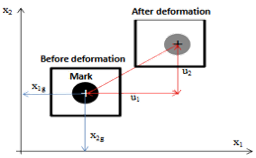
\includegraphics{Figures/Subset_Movement}
%	\decoRule
%	\caption[Subset Displacement]{Tracking markers scheme with the displacement of a mark before and after a deformation}
%	\label{fig:Fig7}
%\end{figure}
%
%The MatchID software was chosen to compute DIC images and obtain displacement field and strain one. It is a powerful software with a new option which is linked to “crack” studies.
%Thanks to this software, some ”.csv” files full of information were available. All the images recorded were treated with MatchID and every picture are divided into a large number of subsets. One subset is composed of 225pixels (square of 15 by 15 pixels). It is possible to have a look on the crack video, watch the different strains modelized by MatchID using every pixel’s evolution. Then the user must determine the initial length. Indeed, even if the specimens were manufactured with a precise shape, it was important to calibrate the initial length of the crack, by choosing the subset the closest to the crack tip.
%When all these steps are done, for each experiment, so each specimen, a database have to be created. In these databases, will be found constant and information as this initial crack length $a_{0}$. Moreover, there is information, common to each test as the specimen geometry, filmed values or conversion factors.
%
%As it is visible on \ref{fig:Fig7} DIC process works as Finit Element Method (FEM). Indeed a subset can be considered as an element of the project and then, looking to his displacement, strains and displacement map can be plot. The next section, will allow to better understand how a comparison between FEM and experiment can be done.
%
%

%\include{Chapters/ChapterExample}
\chapter{Pre and Post processing work preparation}
\label{Pre and Post processing work preparation}


%----------------------------------------------------------------------------------------
%	SECTION 1
%----------------------------------------------------------------------------------------

\section{Abaqus software}

First, the purpose of this work is to compare the behavior of wood species with numerical analysis. That is why the preparation work begin by the modelling of MMCG specimen on Abaqus software. Abaqus allows to model a specimen, create a mesh, adapted to the geometry, initialize a crack, and obtain data from a virtual crack.

%----------------------------------------------------------------------------------------
%	SUBSECTION 1
%----------------------------------------------------------------------------------------

\subsection{Geometry and material creation}

The creation of the specimen follows the MMCG geometry specimen. It is explained in \parencite{Reference7} thesis. The different angles are taken into account and the four holes are created. The notch has a length of 25\si{\milli\meter}. 2D and 3D models were created. A 2.9\si{\milli\meter} line was put to continue the precrack and represent the cutter precrack done experimentally. 

Abaqus allows to create a material by adding his characteristics. In wood case as it is studied in this work, orthotropic characteristics must be inquired. Abaqus asks for a D matrix, defined as in \ref{eq:D matrix}
\begin{equation}
	\left[
	\begin{array}{rrrrrr}
		D_{1111} & D_{1122} & D_{1133} &
		0 & 0 & 0 \\
		D_{1122} &
		D_{2222} &
		D_{2233} &
		0 & 0 & 0 \\
		D_{1133} &
		D_{2233} &
		D_{3333} &
		0 & 0 & 0 \\
		0 & 0 & 0 &
		D_{1212} & 0 & 0 \\
		0 & 0 & 0 & 0 &
		D_{1313} & 0 \\
		0 & 0 & 0 & 0 & 0 &
		D_{2323} \\
	\end{array}
	\right]
	with : \\
	\\
	\left\{
	\begin{array}{lllll}
		D_{1111}=E_{1}(1-\nu_{23}\nu_{32})\gamma \\
		D_{2222}=E_{2}(1-\nu_{13}\nu_{31})\gamma \\
		D_{3333}=E_{3}(1-\nu_{12}\nu_{21})\gamma \\
		D_{1122}=E_{1}(\nu_{21}+\nu_{31}\nu_{23})\gamma \\	D_{1133}=E_{1}(\nu_{31}+\nu_{21}\nu_{32})\gamma	 \\	D_{2233}=E_{2}(\nu_{32}+\nu_{12}\nu_{31})\gamma \\	D_{1212}=G_{12} \\	D_{1313}=G_{13} \\	D_{2323}=G_{23} \\
	\end{array}
	\right.
	\label{eq:D matrix}
\end{equation}
It means that it is necessary before using ABAQUS to determine all these coefficients depending on the specie and the direction of the wood. These values for specimen at 12\% of MC which are the shearing $G_{ij}$ and longitudinal modulus $E_{i}$, the Poisson's coefficient $\nu_{ij}$ and $\gamma$ change for each species. After filling this D matrix it is possible to characterize the material of the specimen modelled. As an example, Okoume specie can be characterized by the values in \ref{eq:Okoume physicals values} which are confirmed by \parencite{Reference5}
\begin{equation}
	\left\{
	\begin{array}{llllllllllll}
		E_{1} = 9634 (MPa) \\
		E_{2} = 1090 (MPa)\\
		E_{3} = 522 (MPa) \\
		\nu_{12} = 0,369 \\
		\nu_{13} = 0,472 \\
		\nu_{23} = 0,705 \\
		\nu_{21} = \nu_{12}\dfrac{E_{2}}{E_{1}} = 0,042 \\
		\nu_{31} = \nu_{13}\dfrac{E_{3}}{E_{1}} = 0,026 \\
		\nu_{32} = \nu_{23}\dfrac{E_{3}}{E_{2}} = 0,338 \\
		G_{12} = 808 (MPa) \\
		G_{13} = 594 (MPa) \\
		G_{23} = 186 (MPa) \\
		\gamma = \dfrac{1}{1-\nu_{12}\nu_{21}-\nu_{13}\nu_{31}-\nu_{23}\nu_{32}-2\nu_{21}\nu_{32}\nu_{13}} = 1,387 \\
	\end{array}
	\right.
	\label{eq:Okoume physicals values}
\end{equation}
These values can evolve due to temperature and relative humidity. This is why, Guitard's model from \parencite{Reference2} are used. Indeed, by knowing the temperature, the relative humidity and the volume weight of a specimen, it is possible to obtain at least nine of the physicals values presented in \ref{eq:Okoume physicals values}. An important factor to obtain these parameters is also the wood type, hardwood or softwood. 

After the creation of the material by inputting the D matrix values. But also values as the density or the expansion coefficient linked to temperature. The material is assigned to the geometrical part.

%--------------------------------------------------------------%---------------
%	SUBSECTION 2
%----------------------------------------------------------------------------------------

\subsection{Load and boundary conditions}
Load and Boundary Condition (BC) must be also inquired. In 2 dimensions, the specimen was considered as blocked from one of the upper side. While the load is applied on the other upper side, even if the applied load is a surface one, localized in the hole as the BC. In 3 dimensions, load and BC are applied in the holes, so it must be closer to experimental conditions. The BC was considered as an embedding, even if in experimental conditions a displacement can occurs on the pin. So then, one dimension is considered as free. The magnitude was chosen at : 10\si{\kilo\newton}. The load type is considered as a "Surface Traction" and the added as a static load in a Global system x,y,z. The distribution is an uniform one and the direction, for this mode I Work, is perpendicular to the crack.

To provide the problem of a crack propagating from the hole, as it appears on some simulations, the area where the load is applied was considered as undeformed. The test expected is a dynamic one, working as an incremental process.

%----------------------------------------------------------------------------------------
%	SUBSECTION 3
%----------------------------------------------------------------------------------------

\subsection{Zone of Interest }
According to the tinny FPZ allows by MMCG geometry, the Zone of Interest must be well chosen. \parencite{Reference7} had already found ZOI shapes that allow the crack propagation study. By adapting the values to the dimensions of this work samples, a square of 2.8\si{\centi\meter} vertically and 5.6\si{\centi\meter} horizontally was created next to the precrack. As visible on \ref{fig:Abaqus_interface}
Then, three areas were also drawn as on \ref{fig:Abaqus_interface} and \ref{fig:Fig4}. The purpose of this ZOI and the 3 zones around the crack tip is to refine the analysis by creating a thinner mesh inside these areas. Indeed, the heel analysis is not relevant in a fracture mechanic problem as the crack study of this work. Whereas the evolution of this 3 areas allows to have a look to the Fracture Process Zone which go further with the time and the crack tip displacement.
One purpose is to obtain the stress concentration factor involves by the crack propagation on this ZOI.

%----------------------------------------------------------------------------------------
%	SUBSECTION 4
%----------------------------------------------------------------------------------------

\subsection{Mesh and link to finite element analysis}
Concerning the mesh, it is special on this geometry. But it will be focused on the crack and around it. The interest is to determine the displacement and the strain applied on the element of the mesh. That is why a ZOI was created \ref{fig:Fig16} and a thinner mesh was done in this area. Indeed, it is the interesting one, where the crack must develop. \parencite{Reference8} presented in the MMCG creation a mesh with element "tri" so triangular ones in many areas of the specimen. This mesh was really interesting because it is a radial one, with a center near the crack tip. It is localized at a constraint point. Moreover, the mesh in this area become a "quad" mesh, so rectangular elements or quadrilateral ones at least. In this work, "quad" elements were chosen.
\begin{figure}[h]
	\centering
	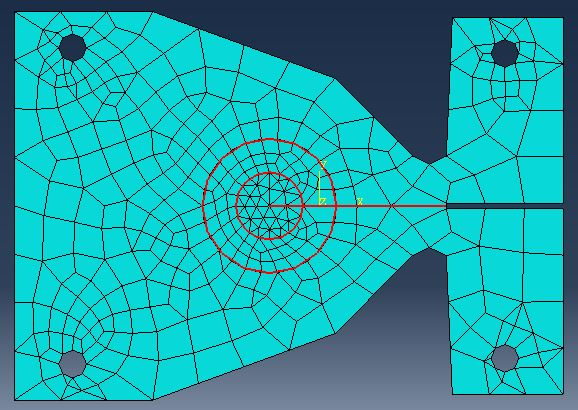
\includegraphics[scale=0.5]{Figures/Abaqus_Screenshot}
	\decoRule
	\caption[ABAQUS 2D specimen]{ABAQUS 2D Okoume specimen meshed with underlined ZOI and crack direction.}
	\label{fig:Fig16}
\end{figure}
Then, a step is created and also a job with the crack developement. This job allows to obtain a representation of the strain in each element of the mesh.
%----------------------------------------------------------------------------------------
%	SECTION 2
%----------------------------------------------------------------------------------------

\section{Python program}

%----------------------------------------------------------------------------------------
%	SUBSECTION 1
%----------------------------------------------------------------------------------------

\subsection{Initialization and input values}

The Python code developed is inspired from a previous one, done in MatLab by \parencite{Reference14} for DCB tests. MMCG specimen was created from DCB one, so it was logical to use this program with an adaptation to Python tools. 

The main purpose of this tool is to compute all the information given by DIC and obtain the energy release rate. To do that, it was reminded in \ref{eq:Energy release rate equation} that many parameters must be input. Some of them are constant and was measured before or after the test. It is the case for $a_{0}$ and "b" parameters, respectively, the initial crack length and the thickness of the specimen analyzed. It is defined in four big parts.

So a first program, allowing to combine all the constants by creating a structure as the one below, was done. It is called database and the following one is the example from the third Okoume specimen of the first experiment database:

\lstinputlisting[language=Python, firstline=1, lastline=9]{Codes/Database.py}

\begin{lstlisting}[language=Python]
	LX, H = 29.3, 1624  # mm / pixel
	if Job == 'e1o3':
	##########################################################################
	# pixel to mm magnification factor
	Test.mm2pixel = LX / H
	# Load conversion factor - testing machine
	Test.LoadConvFactor = 1000  # from kN to N
	# Displacement conversion factor - testing machine
	Test.DisplConvFactor = 2.0  # mm/V (gain = 20 mm)
	Test.thickness = 14 # unit  mm
	Test.a0 = 24.5 # unit  mm
\end{lstlisting}

\lstinputlisting[language=Python, firstline=11, lastline=19]{Codes/Database.py}

Thanks to this database file, open in the main code, many calls can be done and allow to synthesize the main code. Of course one database was created for each specimen and input in a single folder, due to the difference between values as the precrack length or the thickness of the specimen. Other values as the "Test.LoadConvFactor" will always be the same. Indeed, in this work, the load values, given by the MTS press are given in \si{\kilo\newton}, so a coefficient of 1000 must be added to obtain coherents results.

All the values from MatchID must be read and the displacement or load from the servohydraulic test machine have to been stored in Python variables. 

\begin{lstlisting}[language=Python]
	# determining the number of stages by inspecting MatchID processing files
	stages = glob.glob(os.path.join(cwd, 'DCB_002_*.tif.dat'))
	MatchID.stages = stages.__len__()
	print('Number of stages: ', str(MatchID.stages))
\end{lstlisting}

The first step is to store in a parameter, the number of stages by looking to the number of images captured by MatchID. As it is visible, variables are created, in a structure named MatchID. Here, the number of stages is stored in MatchID.stages variable. This MatchID structure is present in the database, because it is linked to each specimen. Indeed, the number of images changes from one test to another. So another part of the database is linked to MatchID settings and add information linked to this structure:  

\begin{lstlisting}[language=Python]
	# Summary of DIC Settings
	MatchID.CorrelationCoef = 'ZNSSD'
	MatchID.InterpolationOrder = 'Bicubic spline'
	MatchID.TransformationOrder = 'Affine'
	MatchID.Subset, MatchID.Step = 15, 13
	# Summary of Strain Settings
	MatchID.StrainWindow = 5
	MatchID.StrainConvention = 'GreenLagrange'
	MatchID.StrainInterpolation = 'Q4'
	# Area of Interest
	MatchID.Roi_PolyXi, MatchID.Roi_PolyYi = 52, 259
	MatchID.Roi_PolyXf, MatchID.Roi_PolyYf = 1587, 1119
\end{lstlisting}

It is possible to use, thanks to this part, the type of subset used, the steps, the strain window and interpolation, previously chosen, looking on the best parameters on MatchID curves. Then, the displacements and load of every stages must be stored to. In order to do it, an iterative loop is created :

\begin{lstlisting}[language=Python]
	# U displacement
	UX = np.zeros((MatchID.SubsetsY, MatchID.SubsetsX, MatchID.stages))
	tic()
	for i in np.arange(0, MatchID.stages, 1):
	readstr = #Name of the test
	print('reading : ',readstr)
	pathdados = os.path.join(cwd,'u',readstr)
	aux = np.genfromtxt(pathdados, skip_header=0, delimiter=';')
	UX[:, :, i] = aux[:, :-1]*Test.mm2pixel # unit: mm
	print(f'{toc():.1f} seg')
\end{lstlisting}

This loop stores the displacement on U direction, but another similar one do the same on V direction. Ux is a Matrix filled by the reading of MatchID.subset file and the number of stages. Then it is multiply by the convector factor from pixel to \si{\milli\meter}. 

%----------------------------------------------------------------------------------------
%	SUBSECTION 3
%----------------------------------------------------------------------------------------

\subsection{Determination of the CTOD} 

After computing all the data from the database, a second part is computed. It is linked to the Crack Tip Opening Displacement (CTOD). Indeed, this factor has impact on the cohesive law. MatchID is a great tool which does some work for the user. That is why, some of the information from the software program were put in the Database, as in the next code with the ZOI dimensions: 
\begin{lstlisting}[language=Python]
	# Allied Manta G-505B
	H, V  = 2448, 2050 # unit: pixels
	# 'TC2336' telecentric lens
	LX, LY = 34.98, 29.18 # unit: mm
\end{lstlisting}

Then, two matrix are created. There are first, declared and made of zeros :

\begin{lstlisting}[language=Python]
	CTODI  = np.zeros((ud_lim, 3, MatchID.stages))
	# Vup, Vdown, ||Vup-Vdown||
	CTODII = np.zeros((ud_lim, 3, MatchID.stages))
\end{lstlisting}

As shown in the code, the dimensions of the matrix take in account the number of stages, so the number of images. Indeed, the interest of the CTOD is to be followed at each stage. 

Then, a loop is created, allowing to put information into others vectors

\begin{lstlisting}[language=Python]
	for J in np.arange(0, MatchID.stages, 1):
	# mode I:
	uYtemp = np.copy(UY[:, :, J])
	CTODI[:, 0, J] = np.flipud(uYtemp[a0.Y - ud_lim: a0.Y, a0.X])
	CTODI[:, 1, J] = uYtemp[a0.Y: a0.Y + ud_lim, a0.X]
	CTODI[:, 2, J] = np.abs(CTODI[:, 1, J] - CTODI[:, 0, J])
\end{lstlisting}

Another one is also created to compared to mode II values. In the current case, the mode II can be approximate around zero, because it is a mode I test. Then all the values are obtained, for each COD pair until $ud_lim$ which is in this case equal to 10. By looking to this different curves, the chosen COD pair is chosen and a curve is plot looking to the values for this parameter chosen by the user. 

\begin{figure}[h]
	\centering
	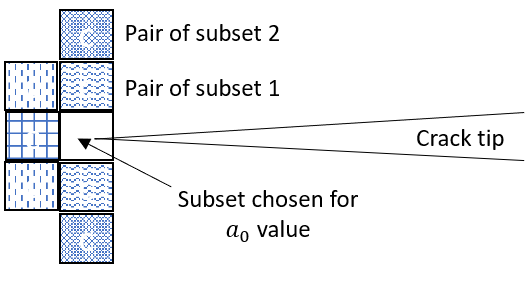
\includegraphics[scale=0.7]{Figures/Subset_choice}
	\decoRule
	\caption[Subset choice and pair of subset around]{Pair of subset around the $a_{0}$ subset chosen}
	\label{fig:subest_chosen}
\end{figure}

Finally, the way to obtain CTOD, need also a well $a_{0}$ choice. Indeed, the chosen subset as presented on \ref{fig:subest_chosen}, will be determinant. Considering the image as a matrix composed of subset, the chosen subset as a position given by his m row and n column. To determinate the opening, it is necessary to have a look on the subsets in the same n column but at a different line. Indeed, the chosen subset will be the first one affected by the crack, that means, that information on the subset will not have importance anymore. While, looking to subset up and down allow to follow the displacement of the crack tip and measure it. The fact is to determine which pair of subsets is the best. The ones at the row n-1 and n+1, but maybe these ones will be on the crack at a given stage, and will lose all the necessary information. That is why, an important choice must be done. Here, COD pair was fixed equal to two. So the subset displacement analysed is the one of the pair of subset 2 on \ref{fig:subest_chosen}. Finally, by looking to these displacements, it is possible to obtain the value of the crack opening at each stages.

%----------------------------------------------------------------------------------------
%	SUBSECTION 4
%----------------------------------------------------------------------------------------

\subsection{Crack length analysis}

The third part of the code has the purpose to determine a(t), so the crack length evolution. This evolution can be compared to the time or the servohydraulic test machine displacement and also the load applied on the specimen. The first step is again to define everything. The displacement are stored again, the Zone Of Interest (ZOI) is defined by suppressing the value out of this ZOI.
This a(t) parameter is the most difficult to obtain, indeed tools as MatchID cannot help the user to obtain the result stage by stage. The value of a(t) will be equal to $a_{0}$ fixed by the user and add to a $\Delta a$ which is the value of the crack length, evolving in time due to the applied force.

\begin{lstlisting}[language=Python]
	displ_x = UX[:,:,J]
	displ_y = UY[:,:,J]
	# resize RoI containing the crack growth process
	if roi == 'crop':
	displ_x = displ_x[Y_i:Y_f,X_i:X_f]
	displ_y = displ_y[Y_i:Y_f,X_i:X_f]
	
	# find the dimensions of the matrix
	m = displ_x.shape[0] #  y - row
	n = displ_x.shape[1] # x - column
	# find the matrix with the displacements
	displ = (displ_x**2 + displ_y**2)**0.5
	# preallocation: zeros
	n_zeros = np.zeros((m, 1))
	m_zeros = np.zeros((1, n+1))
\end{lstlisting}

After defining all the parameters, the displacement of the crack tip is observed thanks to some calculus on the subsets. 

\begin{lstlisting}[language=Python]
	displ_A = np.vstack((np.hstack((displ,n_zeros)), m_zeros))/4
	# divided by 4 because sum: displ_A+displ_B+displ_C+displ_D
	displ_B = np.vstack((np.hstack((n_zeros,displ)), m_zeros))/4
	displ_C = np.vstack((m_zeros, (np.hstack((displ, n_zeros)))))/4
	displ_D = np.vstack((m_zeros, (np.hstack((n_zeros, displ)))))/4
	# auxiliar matrix 2 edges; 4 within the matrix 'matr_transf'
	matr_transf = np.ones((m+1, n+1))
	matr_transf[:, 0] = 2
	matr_transf[:, -1] = 2
	matr_transf[0, :] = 2
	matr_transf[-1, :] = 2
	matr_transf[0, 0] = 4
	matr_transf[0, -1] = 4
	matr_transf[-1, 0] = 4
	matr_transf[-1, -1] = 4
	grid_values = (displ_A + displ_B + displ_C + displ_D)*matr_transf
	# displacements of each corner on the facet
	displ_A = grid_values[0:-1, 0:-1]
	displ_B = grid_values[0:-1, 1:]
	displ_C = grid_values[1:, 0:-1]
	displ_D = grid_values[1:, 1:]
	# oblique distance between facet centroids
	displ_CA = np.abs(displ_C-displ_A)
	displ_DB = np.abs(displ_D-displ_B)
	# auxiliar function for the crack tip location criterion
	K = np.maximum(displ_CA, displ_DB)
	avgK = np.nanmean(K) #mean ignoring nan values.
	stdK = np.nanstd(K)
	maxK = np.nanmax(K)
	if maxK < avgK + inb*stdK:
	J = J + 1
	else:
	JJ = 0
\end{lstlisting}

Here, all the matrix, composed of the subsets from the Zone of Interest are changed by the different steps shown overhead. All the subsets are considered four by four and operations are done on them. The displacement from one compared to it neighbor are computed. Then average and maximum values are obtained for each subset of the ZOI and put into K matrix. By using the $a_{0}$ data and looking to the alpha parameter, permitting to compute the best shape of a(t), having the more precise values but numerous ones also, a(t) is obtained with a similar method. It must be noticed, that to determinate a(t) parameter, $\alpha$ parameter is needed. This one is used on matrix as the M matrix. Indeed, M matrix represents, for a given stage, the crack length by having bigger value in the crack area as shown on \ref{fig:Fig11} : 

\begin{figure}[h]
	\centering
	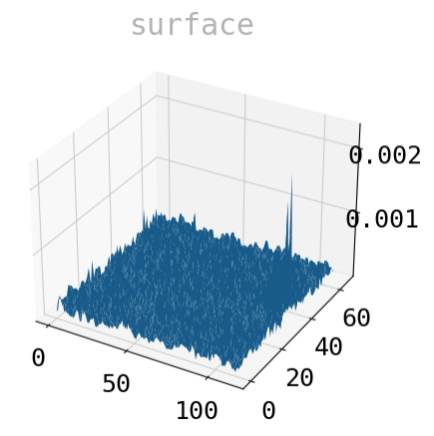
\includegraphics[scale=0.5]{Figures/M_matrix}
	\decoRule
	\caption[M matrix]{M matrix, obtained by running python code}
	\label{fig:Fig11}
\end{figure}

As it is visible, if the user is looking too close, the noise of the values will avoid a good analyze, but by looking too high on the matrix, the crack length value will not be accurate. To move and have a precise idea of the way the user can watch the M matrix, it is important to use $\alpha$. Alpha parameter is like a cutting tool which allows to be as close as the noise without troubles.
To approximate the $\alpha$ value, a correlation factor is searched by least square regression method. The objective it to have the best linear part. A plot is created to show which stage is the most appropriate as on \ref{fig:Fig12}.

\begin{lstlisting}[language=Python]
	### 2 criterion for checking stage
	####
	inb = 3
	# standard deviation * inb (to be checked by user)
	# inb = 1: 68.3 %
	# inb = 2: 95.4 %
	# inb = 3: 99.7 %
\end{lstlisting}

It is possible to adapt the alpha parameter precision by choosing a different "inb" as presented in the code overhead. Indeed, the correlation factor change depending on this criterion. The chosen stage is the one, before the beginning of the crack propagation, but the nearest to the expansion of a(t) length.

\begin{figure}[h]
	\centering
	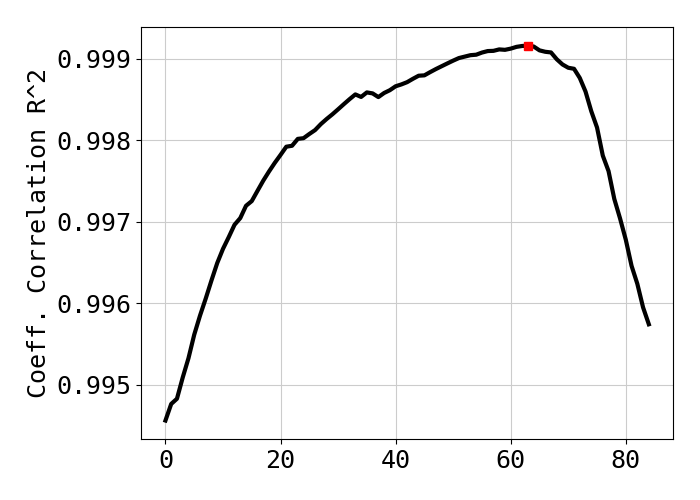
\includegraphics[scale=0.3]{Figures/Correlation_factor}
	\decoRule
	\caption[R correlation factor]{R correlation factor allowing to know which load and displacement is linked to crack beginning.}
	\label{fig:Fig12}
\end{figure}

This method was the one used by \parencite{Reference14} on MatLab, and have already proved obtention of good results.

%%----------------------------------------------------------------------------------------
%%	SUBSECTION 5
%%----------------------------------------------------------------------------------------
\subsection{Compliance and Energy values}

The last part of the code consists in using all the calculated parameters, in order to obtain the energy release rate. It is done by computing the G formula as presented below.

\begin{equation}
	G_{c}= \frac{F_{c}^2}{2b} (\frac{\Delta C}{\Delta a})_{d} 	
	\label{eq:Energy release rate equation}
\end{equation}

This equation, already given, is written on Python as :

\begin{lstlisting}[language=Python]
	a_t = crackL_J_mm[:,chos_alp]
	
	C = MatchID.displ/MatchID.load
	
	# P**2/2/B* dC / da
	ALP = (MatchID.load**2)/(2*Test.thickness)
	
	# C = MatchID.displ/MatchID.load
	
	# BET = C/a_t #changing the value of alpha from the crack length will change G values
	#
	G = ALP*BET
	# G = np.dot(ALP,BET)
\end{lstlisting}

In this case, the formula used, is the simplest one, which allow to easily obtain C by dividing the displacement from servohydraulic test machine by the load. These values are stored in MatchID variable, allowing to synthesize all the data in one per image (stage). An average are done on the seven values between two images. This fact can also involve a little mistake.
Therefore, as explained in "alpha" and "a(t) determination" sections, the crack length depends on alpha parameter. So some curves are plotted depending on "a(t)" matrix changes according to the alpha. The best R-curves must be determined for the most precise crack length. So it is necessary to find a great alpha parameter to have these final values without huge mistake.

\begin{lstlisting}[language=Python]
	# write array results on a csv file:
	RES = np.array([MatchID.displ[:], MatchID.load[:], C[:], COD.wI[:], a_t[:], G[:]])
	RES = np.transpose(RES)
\end{lstlisting}

At least, values as the displacement, the load, the compliance, the CTOD, the crack length and the energy release rate, are stored into a matrix and then exported to .csv files. It allows saving data, but also to compute everything in Excel in addition to python processing tool.

Many improvements are made on the Python code, even after this work ended. Indeed, it appears that the crack length can be better compute, in order to avoid some strange shapes of R-curves. But using the same tool for all specimens computation, even if mistakes exist, it is possible to compare data.


%\section{Python program}
%
%%----------------------------------------------------------------------------------------
%%	SUBSECTION 1
%%----------------------------------------------------------------------------------------
%
%\subsection{Initialization and input values}
%
%The Python code developed is inspired from a previous one, done in MatLab by \parencite{Reference14} for DCB tests. MMCG specimen was created from DCB one, so it was logical to use this program with an adaptation to Python tools. A first program, allows to combine all the constants by creating a structure as :
%
%\begin{customFrame}
%	# pixel to mm magnification factor
%	Test.mm2pixel = LX / H
%	# Load conversion factor - testing machine
%	Test.LoadConvFactor = 50  # N/V (gain = 500 N)
%	# Displacement conversion factor - testing machine
%	Test.DisplConvFactor = 2.0  # mm/V (gain = 20 mm)
%	Test.thickness = 12.5 # unit  mm
%	Test.a0 = 20 # unit  mm
%	###################################################
%	# Summary of DIC Settings
%	MatchID.CorrelationCoef = 'ZNSSD'
%	MatchID.InterpolationOrder = 'Bicubic spline'
%	MatchID.TransformationOrder = 'Affine'
%	MatchID.Subset, MatchID.Step = 15, 13
%	# Summary of Strain Settings
%	MatchID.StrainWindow = 5
%	MatchID.StrainConvention = 'GreenLagrange'
%	MatchID.StrainInterpolation = 'Q4'
%	# Area of Interest
%	MatchID.Roi_PolyXi, MatchID.Roi_PolyYi = 52, 259
%	MatchID.Roi_PolyXf, MatchID.Roi_PolyYf = 1587, 1119
%	###################################################
%	# Selecting subset directly from MatdhID
%	a0.imgH, a0.imgV = 1529, 669
%	# Selecting pair
%	COD.cod_pair = 2
%	
%\end{customFrame}
%
%Thanks to this database file, open in the main code file, many calls can be done and allow to synthesize the main code. Of course one database was created for each specimen, due to the difference between values as the precrack length or the thickness of the specimen. Other values as the "Test.LoadConvFactor" will always be the same. Indeed, in this work, the load values, given by MTS servohydraulic test machine are given in \si{\kilo\newton}, so a coefficient of 1000 must be added to obtain coherent results.
%
%This main code is composed of several parts. First, after defining modules, path and opening all the necessary files as displacement csv file or strain one, it is important to read all the images from a single test. Indeed, it allows to know the number of stages (images) which must be run to obtain the entire test. Each stage gives a displacement of pixels, so un displacement of subsets, allowing to follow the crack length and the crack opening. It is important to note that MatchID allows to focus on a Zone of Interest (ZOI) in order to limit the amount of subsets read. According to \parencite{Reference7} dimensions of this ZOI are given for biggest specimens. By using equivalent dimensions, the ZOI adapted to this thesis is around 5,6\si{\centi\meter} length from the upper holes of the specimen and 2,8\si{\centi\meter} of width.
%
%Then, by using the displacement depending on the axis, x and y, two folders are read, one with x displacements, the other with y displacements. In each folder, one test is composed of a number of files equal to the number of stages. It gives information about pixel movement. By reading these two folders, a first graphic is created, giving a representation of the specimen, with the subsets presented and the subset chosen to be the $a_{0}$ one (closer to the crack tip).
%
%%----------------------------------------------------------------------------------------
%%	SUBSECTION 2
%%----------------------------------------------------------------------------------------
%
%\subsection{Alpha parameter}
%
%To begin with, it is important to determinate a parameter, that we had called $\alpha$. This one is used on matrix as the M matrix. Indeed, M matrix represents, for a given stage, the crack length by having bigger value in the crack area as shown on \ref{fig:Fig11} :
%
%\begin{figure}[h]
%	\centering
%	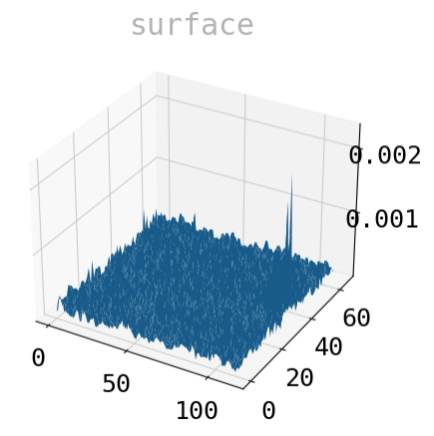
\includegraphics[scale=0.5]{Figures/M_matrix}
%	\decoRule
%	\caption[M matrix]{M matrix, obtained by running python code}
%	\label{fig:Fig11}
%\end{figure}
%As it is visible, if the user is looking too close, the noise of the values will avoid a good analyze, but by looking too high on the matrix, the crack length value will not be accurate. To move and have a precise idea of the way the user can watch the M matrix, it is important to use $\alpha$. Alpha parameter is like a cutting tool which allow to be as close as the noise without troubles.
%To approximate the $\alpha$ value, a correlation factor is searched by least square regression method. The objective it to have the best linear part.
%\begin{customFrame}
%	#### alpha evaluation
%	### Selecting stage for investigating alpha
%	####
%	# least-squares linear regression
%	porder = 1
%	xx = Test.disp # displacement (mm)
%	yy = Test.load # load (N)
%	# Data point in the linear least-squares regression
%	limsup = int(0.75*np.argwhere(max(yy)==yy)[-1])
%	# number of maximum data points for LSR
%	liminf = int(np.round((1/3)*limsup))# number of minimum data points for LSR
%	
%	xx, yy = xx[0:limsup], yy[0:limsup]
%	Rtot = np.zeros((limsup-liminf,1))
%	C_M = np.zeros((limsup-liminf,1))
%	for j in np.arange(0,limsup-liminf,1):
%	limt_sup = liminf + j
%	xfit, yfit = xx[0:limt_sup], yy[0:limt_sup]
%	p  = np.polyfit(xfit, yfit, porder)
%	C_M[j] = 1/p[0]
%	dev = yfit - np.mean(yfit) # deviations - measure of spread
%	SST = np.sum(dev**2) # total variation to be accounted for
%	resid = yfit - np.polyval(p, xfit) # residuals - measure of mismatch
%	SSE = np.sum(resid**2) # variation NOT accounted for
%	Rtot[j] = 1 - SSE/SST #  variation NOT accounted for
%	
%	# position for the best fitting point parameters
%	jmax = np.max(np.argwhere(np.max(Rtot)==Rtot))
%	J = int(liminf + jmax)
%	
%	### 2 criterion for checking stage
%	####
%	inb = 3
%	# standard deviation * inb (to be checked by user)
%	# inb = 1: 68.3 %
%	# inb = 2: 95.4 %
%	# inb = 3: 99.7 %
%	JJ = 1
%	while JJ == 1:
%	\end{customFrame}
%	
%	\begin{figure}[h]
%	\centering
%	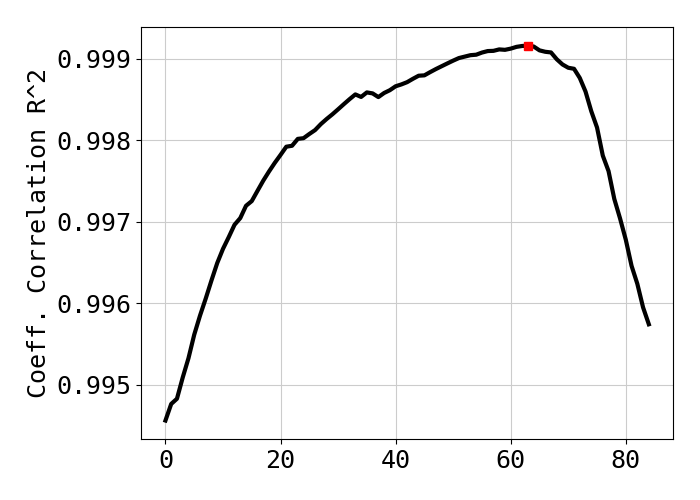
\includegraphics[scale=0.3]{Figures/Correlation_factor}
%	\decoRule
%	\caption[R correlation factor]{R correlation factor allowing to know which load and disalcement is linked to crack beggining.}
%	\label{fig:Fig12}
%	\end{figure}
%	
%The red dot shown on \ref{fig:Fig12}, is linked to another plot,
%	
%Then a matrix representing the subsets in the Area of Interest will be created. First this matrix is composed of zero. Then, the four corners of the matrix will be used to proceed several operations on the matrix. The external lines and columns will take a value of 2 and the corners a value of 4. The distance between opposite corners is calculated and their displacements are compared. Calling K, the maximal displacement of the two corners, average K and maximum one between all the steps are compared. Again, every subset is treated and are still zero when the material is undamaged. It becomes -1 in a region where the material is damaged, and no information are treatable. And it becomes 1 where a discontinuity appears but the wood is not completely damaged like the crack tip. So, by following the farthest 1 value in the matrix, it is possible to know the last subset where the crack tip is localized. Thanks to this distance, some conversions are necessary, from subset to pixel first, and then from pixel to millimeters. Finally, the crack length is determined depending on stages so it could be linked to load or displacement, and thanks to the previous work, to CTOD. The compliance is calculated by dividing the displacement by the load. G is the last variable calculated, with all the previous variables determined, as CTOD presented below and a(t). The last plot is the R-curve representing the Energy release and the crack length.
%%----------------------------------------------------------------------------------------
%%	SUBSECTION 3
%%----------------------------------------------------------------------------------------
%
%\subsection{Determination of the CTOD}
%
%Another partof the code has the purpose to calculate the Crack Tip Opening Displacement (CTOD). MatchID is a great tool which does some work for the user. That is why, by using “wI aramis2D.csv” CTOD is almost find, depending on the time and the load applied. It is important to understand how it works.
%
%First, a part of the work is to define the zone of interest (ZOI), the one where the crack must develop. It is done on MatchID, but also on Python by using the number of the subset defined by Match ID. Then, when a subset is out of this region, it will be considered as equal to zero. Then, the subsets which are placed into the crack, or somewhere where there is a default or missing information as into the crack, the substep will be defined with a value equale to -1. Then, for all the substep around the crack, which have a real interest in the study, they will take the value equal to 1. By using this matrix of substep, now, composed of -1, 0, 1 value, it is possible to plot the entire matrix into grey nuances, and have a look at the crack development, by adding matrix, given by different stages.
%
%\begin{customFrame}
%ud_lim = 10
%# Uup, Udown, ||Uup-Udown||
%CTODI  = np.zeros((ud_lim, 3, MatchID.stages))
%
%for J in np.arange(0, MatchID.stages, 1):
%# mode I:
%uYtemp = np.copy(UY[:, :, J])
%CTODI[:, 0, J] = np.flipud(uYtemp[a0.Y - ud_lim: a0.Y, a0.X])
%CTODI[:, 1, J] = uYtemp[a0.Y: a0.Y + ud_lim, a0.X]
%CTODI[:, 2, J] = np.abs(CTODI[:, 1, J] - CTODI[:, 0, J])
%COD.wI = CTODI[COD.cod_pair, 2, :]
%\end{customFrame}
%
%\begin{figure}[h]
%	\centering
%	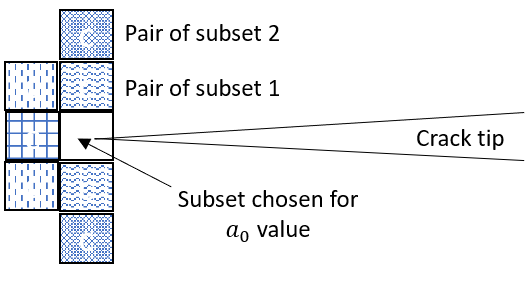
\includegraphics[scale=0.7]{Figures/Subset_choice}
%	\decoRule
%	\caption[Subset choice and pair of subset around]{Pair of subset around the $a_{0}$ subest chosen}
%	\label{fig:subest_chosen}
%\end{figure}
%
%To obtain CTOD, it is important to be careful to $a_{0}$ choice. Indeed, the chosen subset as presented on \ref{fig:subest_chosen}, will be determinant. Considering the image as a matrix composed of subset, the chosen subset as a position given by his m row and n column. To determinate the opening, it is necessary to have a look on the subsets in the same n column but at a different line. Indeed, the chosen subset will be the first one affected by the crack, that means, that information on the subset will not have importance anymore. While, looking to subset up and down allow to follow the displacement of the crack tip and measure it. The fact is to determine which pair of subsets is the best. The ones at the row n-1 and n+1, but maybe these ones will be on the crack at a given stage and will lose all the necessary information. That is why, an important choice must be done. Here COD pair was fixed equal to two. So the subset displacement analyzed is the one of the pair of subset 2 on \ref{fig:subest_chosen}. Finally, by looking to these displacements, it is possible to obtain the value of the crack opening at each stages.
%
%%----------------------------------------------------------------------------------------
%%	SUBSECTION 4
%%----------------------------------------------------------------------------------------
%
%\subsection{Crack length analysis}
%
%At least, an important step in this code is the determination of $a_{DIC}$. This parameter is the crack length, which evolves with time during all the experiment. This factor is the most difficult to obtain, indeed tools as MatchID cannot help the user to obtain the result stage by stage. The value of a(t) will be equal to $a_{0}$ fixed by the user and additional to a $\Delta a$ which is the value of the crack length, evolving in time due to the applied force.
%
%\begin{customFrame}
%roi = 'crop' # 'all'; 'crop'
%i, incr = 1, 1
%# incr : is used to step over stages if required (default = 1: all stages)
%Y_i, Y_f = 0, UY.shape[0]
%X_i, X_f = 0, a0.X
%\end{customFrame}
%
%\begin{customFrame}
%	# estimation of crack tip length
%	tipstep = np.zeros((alphaint.shape[0],1)) # unit: substep
%	tipmm = np.zeros((alphaint.shape[0],1)) # unit: mm
%	
%	for kk in np.arange(0,alphaint.shape[0],1):
%	alpha = alphaint[kk]
%	# Criterion for crack tip location
%	Kt = np.zeros(K.shape)
%	Kt[np.isnan(K)] = -1
%	Kt[K>=alpha*avgK] = 1
%	Ktemp = Kt
%	# n1 which must be relative to 'a0'
%	ind = np.argwhere(Ktemp==1)
%	row, col = ind[:,0], ind[:,1]
%	if len(col) == 0:
%	tipstep[kk] = 0
%	else:
%	tipstep[kk] = a0.X - np.min(col) # X component
%	# pixel>mm: [macro-pixel*(pixel/macro-pixel)*(mm/pixel)
%	tipmm[kk] = np.abs(tipstep[kk]*MatchID.mm2step - MatchID.mm2step)
%	
%	# for selected  alpha parameters you compute crack length
%	# crack length however should be ZERO at the beginning (no crack propagation)
%	ind = np.where(np.abs(tipmm - np.min(tipmm)) == 0)
%	alpha_alphasel = alphaint[ind[0][0]]
%	\end{customFrame}
%A final part of the code allows to obtain a(t) depending on alpha  as it is done on \parencite{Reference14} article. It is done by a focus on the ZOI and the number of subsets composing it. Thanks to the matrix composed by every subsets, the displacement field can be observed. It is obtained by computing the distance between the center of a subset and it displacement from one image to the next one as shown in the literature review. To simplify the code, it is not done on every subset but only on the four corners. By computing the distance between the opposite corners, the maximum x-displacement and an y-displacement are input in a last matrix. 
%
%%----------------------------------------------------------------------------------------
%%	SUBSECTION 5
%%----------------------------------------------------------------------------------------
%
%\subsection{Compliance and Energy values}
%
%As said in alpha parameter section, The last step is to compute the Compliance and then the Energy release rate. Indeed, all the necessary parameters are present in the Python variables. So by computing the formula \ref{eq:Energy release rate equation} the different matrix composed of all the values depending on the stage are used to obtain first a compliance matrix with same dimensions of the CTOD and the dispacement of the servohydraulic test machine matrix created.
%
%As presented in this part of the code, after calculating G, some plots are created. But as explained in "alpha" and "a determination" sections, the crack length depends on alpha parameter. So some curves are ploted depending on "a" matrix changing according to the alpha.And the best R-curves must be determined for the best crack length. It is necessary to find the best alpha parameter to have these final values.
%
%Finaly, 
%----------------------------------------------------------------------------------------
%	SECTION 3
%----------------------------------------------------------------------------------------

\section{Experimental devices}


%----------------------------------------------------------------------------------------
%	SUBSECTION 1
%----------------------------------------------------------------------------------------

\subsection{Arcan model and Final Grips}

MMCG specimens were created to be tested in every fracture mechanics modes. But as presented in the literature review, to be tested in every mode, the load must be applied in different direction. That is why the first grips designed were Arcan ones. Indeed, by changing the way of fixation between each part, it is possible to applied load with 10\textdegree of difference between each fixation point. Thanks to Catia software, the same prototype as the one used by \parencite{Reference7} and \parencite{Reference6} was created as on \ref{fig:Arcan}.

\begin{figure}[h]
	\centering
	\begin{subfigure}{0.48\linewidth}
			\centering
			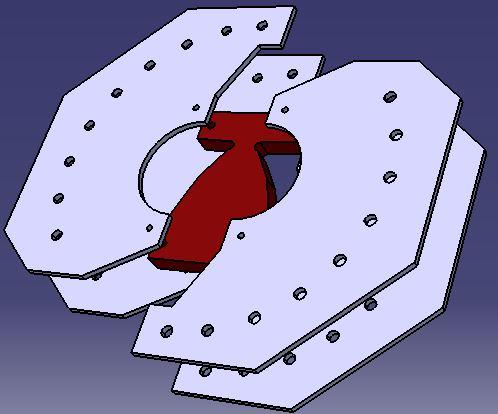
\includegraphics[scale=0.5]{Figures/Result}
			\decoRule
			\caption[Arcan grips]{Arcan design on Catia software}
			\label{fig:Arcan}
	\end{subfigure}
	\hfill
	\begin{subfigure}{0.48\linewidth}
		\centering
		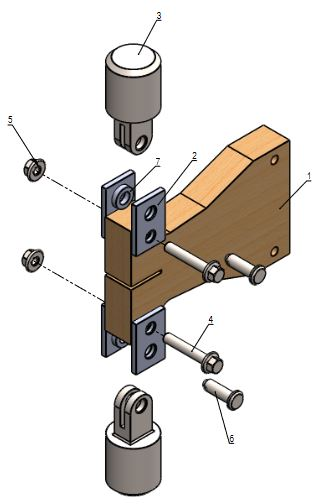
\includegraphics[scale=0.4]{Figures/Grips_model}
		\decoRule
		\caption[Grips modelled]{Mode I grips model composed of 1 : the wood part, 2 : plates 2ISO 4162 - M5 x 30 x 16-C, 3 : Screw part 34 CrNiMo 6, 4 : screw fixing spcimen, 5 : nut, 6 : pin, 7 : washers}
		\label{fig:Grips_model}
	\end{subfigure}
	\hfill
	\begin{subfigure}{0.48\linewidth}
		\includegraphics[scale=0.04]{Figures/Grips}
		\decoRule
		\caption[Grips]{Grips used to connect the Hydraulic press to the spcimen.}
		\label{Grips}
	\end{subfigure}
	\caption{Grips components evolution}
	\label{Grips components evolution}
\end{figure}

In addition with screw and nut placed in the heel holes and, in the case of this work, in the 90\textdegree Arcan system holes, mode I experiments could be done. But this work is focusing on mode I and do not need this heavy plates of steel or PVC in the case of \parencite{Reference8} works.

So the final grips are presented in \ref{fig:Grips_model} and \ref{Grips}. These ones, simpler than ARCAN system, only allow to do mode I experiments. They were designed especially for MMCG dimensions and manufactured near Caparica campus. The system is composed of a main piece which can be added in the mechanical press by screwing it inside. Then, a pin allows to place two connectors from each side of the MMCG specimen. It was induced that the connectors, if they were well tight, could play washers role. Indeed, \parencite{Reference7} as shown the importance of glued washers to provide a crack from the holes. Finally, another pin goes through the connectors and the specimen holes. Experiments have shown that washers are still essential, so they were added as it is visible on \ref{fig:Grips_model} second caption.

It must be noted that, due to the pandemic situation, the grips have taken time to be designed and received. Due to this delay, the experiments have begun only in June.

%----------------------------------------------------------------------------------------
%	SUBSECTION 2
%----------------------------------------------------------------------------------------

\subsection{Servohydraulic test machine used}


To determine the load speed, the frequency of the camera recording and others experimental parameters, it was important to read previous works on the subject and determine which engines will be used to proceed the experiments. The hydraulic press used to pull on each side of the specimen is shown on \ref{fig:HydrauPress}, it is the MTS servohydraulic test machine, model 661.21B-03 allowing a maximal applied load of 100 \si{\kilo\newton}

\begin{figure}[th]
	\centering
	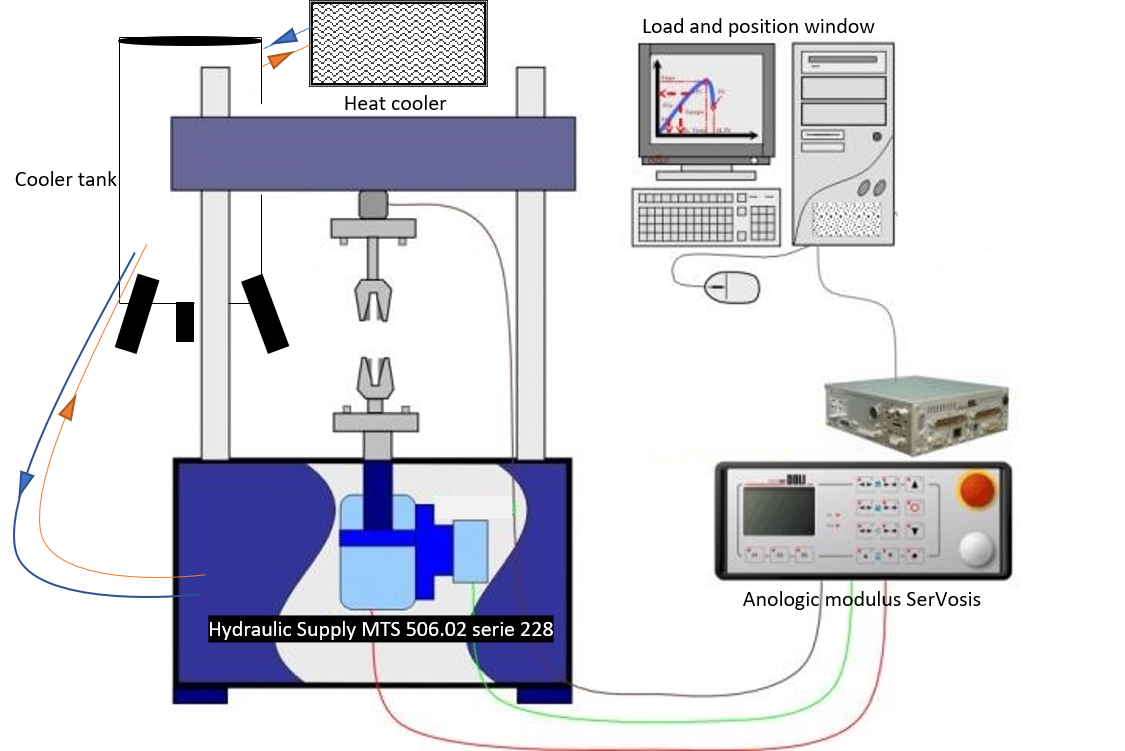
\includegraphics[width=\textwidth]{Figures/Hydraulic_Press2}
	\decoRule
	\caption[Hydraulic Press fonctionnement]{Hydraulic Press components allowing it use}
	\label{fig:HydrauPress}
\end{figure}
	
\parencite{Reference17} works allow to find how the load must be applied. Indeed, it gives an approximation of loads values or displacement speed. The load speed recommended is about 0,1\si{\milli\meter\per\minute} according to these texts. \parencite{Reference7} used the same loading speed around 5\si{\milli\meter\per\minute}. The records are made at a frequency of 5Hz, so 5 images per second, according to \parencite{Reference17} or \parencite{Reference16}.
\parencite{Reference7} works helps to specify this type of parameters on MMCG samples. It is obvious that there are many similitude with DCB works. Indeed, MMCG geometry is an adaptation of DCB and CTS ones, that explain why many parameters are the same. It must be reminded that this press is also chosen because of this possibilities to load specimens by a constant time displacement. Indeed, it was explained that this work will use complacency method to compare the results.


This MTS servohydraulic test machine works in addition with a cooler fluid. Indeed, in a room close to the testing one, a tank full of fluid mixed to water and a cooler system send this fluid mix to the press as visible on \ref{fig:HydrauPress}. Then a hydraulic supply from MTS company send this liquid to the press itself. It is  the model 506.02 serie 22 coupled with the Vickers DG4V-3-2A. Then the pressure is created thanks to the Hydraulic Service Manifold part from MTS company, model 234.11. Finally, a servo valve MOOG A076-263c increase the pressure to allow the hydraulic press operation. It is a high performance valve which covers a rated flow of 4 to 58 \si{\liter\per\minute} which drives a dry torque motor. Then a MTS load cell (661-21B-03) allows to follow the displacement of the servohydraulic test machine. 

%----------------------------------------------------------------------------------------
%	SECTION 4
%----------------------------------------------------------------------------------------

\section{Specimen preparation}

To begin with, all the specimens were named as presented in \ref{tab:Tab3}. It helps, to follow the evolution of each sample.
In this document, these names will be used. Their composition are made of the number of the experiment :
\newline
E1 : Test at a room temperature and a room MC
\newline
E2 : Test at a room temperature and specimens with 30\% MC
\newline
E3 : Test at a room temperature and specimens with 20\% MC
\newline
E4 : Test at a cooler temperature
\newline
E5 : Test at a hotter temperature
\newline
F : Test with Fatigue loads
\newline
Pbis/Pter : are 2 others specimens which were used to calibrate the tests
\newline
\newline
Then the name as a second component, which is the specie and the number of the specimen of this specie dedicated to this test.
\newline
O : Okoume
\newline
P : Padouck
\newline
I: Iroko
\newline
\newline
Finally, all the specimens are named like E1O1 which is the first specimen of Okoume used for the first type of experiment (room temperature and MC due to relative humidity in the air). These names were first written on specimens, but they disappeared when the specimens were put into water. So finally, names were engraved with a cutter.

%----------------------------------------------------------------------------------------
%	SUBSECTION 1
%----------------------------------------------------------------------------------------

\subsection{Notch and Precrack}

Then, notches were created in each specimen. A precrack is made by a cutter into the notch. The interest is to initiate a straight crack, thanks to this first one. The notch width is around 1.5\si{\milli\meter}, done by a straight electrical saw : the Dexter Power NC500JS, and a blade of 1.27\si{\milli\meter}. Then the cutter allow to go deeper and create a precrack with a shape allowing the propagation of the crack. The precrack must be done at the center of the sample heel. Indeed, even a little eccentricity could cause a deviation of the crack and prevent a good study of the propagation. It is easier to do that on a numerical tool than with a saw. Despite a following line draw on the sample, some specimens present a one or two millimeter eccentricity. 

As a logical fact involves by species different density, the creation of the notch was not as easy as expected. Padouck specie, which is, again, the denser, was really difficult to cut. The electrical saw involved smoke and a burnt smell, then cutter precrack was not as uniform as desired. Indeed, even if the tested surface looks cut, into the material, it is impossible to be sure that the precrack cross the entire specimen. A solution found was to compare the surface measured precrack, to real precrack measured after specimen collapse. As visible on \ref{fig:Precrack} the notch is really straight at the contrary of the real precrack and it is a significant delta. By looking to the average precrack composed of the surface precrack length and the central one, \ref{tab:Tab11} presents all the dimensions of the used precracks.
\begin{figure}[h]
	\centering
	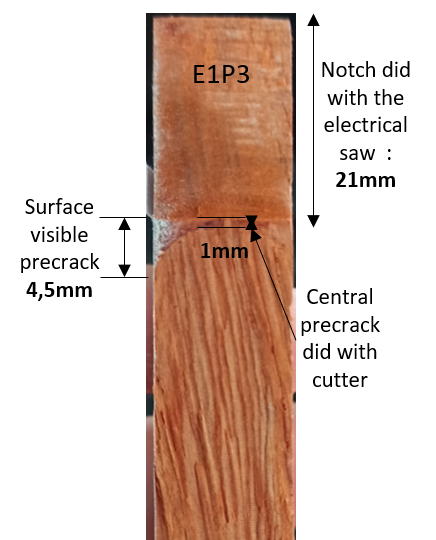
\includegraphics[scale=0.8]{Figures/Precrack}
	\decoRule
	\caption[Collapsed specimen]{Collapsed E1P3 specimen allowing to observe the real precrack length}
	\label{fig:Precrack}
\end{figure}

\begin{table}[h]
	\centering
	\begin{tabular}{c c }
		\multicolumn{1}{l}{} & \multicolumn{1}{l}{Used initial Crack length} \\
		\multicolumn{1}{c}{\cellcolor[HTML]{F8CBAD}E1O1} & 24,975   mm \\
		\multicolumn{1}{c}{\cellcolor[HTML]{F8CBAD}E1O2} & 24,25 mm \\
		\multicolumn{1}{c}{\cellcolor[HTML]{F8CBAD}E1O3} & 24,5 mm \\
		\multicolumn{1}{c}{\cellcolor[HTML]{C65911}E1P1} & 23,25 mm \\ 
		\cellcolor[HTML]{C65911}E1P2 & 23,4 mm \\ 
		\cellcolor[HTML]{C65911}E1P3 & 23,5 mm \\ 
		\multicolumn{1}{c}{\cellcolor[HTML]{BF8F00}E1I1} & 24,975 mm \\ 
		\multicolumn{1}{c}{\cellcolor[HTML]{F8CBAD}E2O1} & 26,475 mm \\ 
		\multicolumn{1}{c}{\cellcolor[HTML]{F8CBAD}E2O2} & 27,975 mm \\ 
		\multicolumn{1}{c}{\cellcolor[HTML]{F8CBAD}E2O3} & 29 mm \\ 
		\multicolumn{1}{c}{\cellcolor[HTML]{C65911}E2P1} & 27,4 mm \\ 
		\multicolumn{1}{c}{\cellcolor[HTML]{C65911}E2P2} & 27,9 mm \\ 
		\multicolumn{1}{c}{\cellcolor[HTML]{C65911}E2P3} & 27,5 mm \\ 
		\multicolumn{1}{c}{\cellcolor[HTML]{F8CBAD}E3O1} & 21,475 mm \\ 
		\multicolumn{1}{c}{\cellcolor[HTML]{F8CBAD}E3O2} & 22,75 mm \\ 
		\multicolumn{1}{c}{\cellcolor[HTML]{F8CBAD}E3O3} & 21,975 mm \\ 
		\multicolumn{1}{c}{\cellcolor[HTML]{C65911}E3P1} & 21,9 mm \\
		\multicolumn{1}{c}{\cellcolor[HTML]{C65911}E3P2} & 20,5 mm \\ 
		\multicolumn{1}{c}{\cellcolor[HTML]{C65911}E3P3} & 24,6 mm \\ 
		\multicolumn{1}{c}{\cellcolor[HTML]{F8CBAD}E4O1} & 23,975 mm \\ 
		\multicolumn{1}{c}{\cellcolor[HTML]{C65911}E4P1} & 23,25 mm \\ 
		\multicolumn{1}{c}{\cellcolor[HTML]{BF8F00}E4I1} & 23,975 mm \\ 
		\multicolumn{1}{c}{\cellcolor[HTML]{F8CBAD}E5O1} & 24 mm \\ 
		\multicolumn{1}{c}{\cellcolor[HTML]{C65911}E5P1} & 22,75 mm \\ 
		\multicolumn{1}{c}{\cellcolor[HTML]{BF8F00}E5I1} & 23,975 mm \\ 
		\multicolumn{1}{c}{\cellcolor[HTML]{C65911}Pbis} & 23,9 mm \\ 
		\multicolumn{1}{c}{\cellcolor[HTML]{C65911}Pter} & 23,25 mm \\ 
\end{tabular}
\caption{Precrack dimensions}
\label{tab:Tab11}
\end{table}
These values were obtained by the comparison of the surface precrack measured first and the look to the real precrack on \ref{fig:Precrack}. The equation used is shown in \ref{eq:precrack determination} :
\begin{equation}
	\centering
	\begin{array}{l}
		a_{0}= l_{notch} + \frac{l_{surfacic}+l_{interior}}{2}
		\\
		\\
		\left\{
		\begin{array}{llll}
			a_{0}: & $initial crack length$ & \si{\milli\meter} \\
			l_{notch}: & $notch length$ & \si{\milli\meter} \\
			l_{surfacic}: & $surfacic precrack measured$ & \si{\milli\meter} \\ 
			l_{interior}: & $real interior precrack measured$ & \si{\milli\meter} \\
		\end{array}
		\right.
	\end{array}
	\label{eq:precrack determination}
\end{equation} 
For some of the specimens, the crack was not done until the entire collapse. Then an approximation was made, using the average of the difference between the initial crack length measured and the one using \ref{eq:precrack determination} to have a more precise value. The average was made for each specie. Indeed, the average of this difference for Okoume specimen is around 1.525\si{\milli\meter} while the one for Padouck is 1.6\si{\milli\meter}. So this value was subtracted from the first measure, in order to take count of the non-uniform precrack.
All the specimens were weighed again, due to the material taken away by the creation of the notch.
%----------------------------------------------------------------------------------------
%	SUBSECTION 2
%----------------------------------------------------------------------------------------

\subsection{Moisture Content determination}

The literature review as shown some ways to determine the MC in specimens. The best way is to put specimens in a climatic room and wait until specimens have reached the expected MC thank to given climatic conditions input in the climatic room controller. Then a moisture meter can give instantly the MC into each sample. 

Without all this equipments, the formula \ref{eq:Moisture content depending on weight} is used. It means that many weight measurements must be done. 

So the 30 specimens bring from Polytech laboratory was weighed as soon as the sanitary condition (Covid pandemic) allows to do it. The scale used to weight the specimen was really precise, it is the GR-200 which is a Semi-Micro Analytical Balances. This precision is also made by the subtraction of air in the glass box, allowing a precision with the thousandths gram as visible on \ref{fig:Fig9}. Its capacity can not reach 210g which does not affect the measures with a max weight of the denser wood, the Padouck, around 70.5g and a minimum weight of Okoume specimens with a weight of 36g
\begin{figure}[th]
	\centering
	\includegraphics[scale=0.05,angle=-90]{Figures/Balance_Test}
	\decoRule
	\caption[GR-200 Scale]{GR-200 Scale weighing an Okoume specimen}
	\label{fig:Fig9}
\end{figure}

After this analyze, weight values were inputted in an Excel file. A resume is presented below in \ref{tab:Tab1} but the entire one is \ref{tab:Tab3}

\begin{table}[h]
\centering
\begin{tabular}{c r}
	\hline
	\cellcolor[rgb]{ .973,  .796,  .678}
	okoume average weight &
	\cellcolor[rgb]{ 1,  1,  1}
	40,55 g \\
	\cellcolor[rgb]{ .776,  .349,  .067}
	padouck average weight &
	\cellcolor[rgb]{ 1,  1,  1}
	66,29 g \\
	\cellcolor[rgb]{ .749,  .561,  0}
	iroko average weight &
	\cellcolor[rgb]{ 1,  1,  1}
	54,33 g \\
	\hline
\end{tabular}
\caption[specimens average weight]{specimens average weight depending on the species}
\label{tab:Tab1}
\end{table}
The next step was to dry them, in order to obtain the $M_{0}$ parameter, essential to approximate the MC. A drying process was done on all the specimens during 24h at 103\textcelsius. The scale was not the same and some specimens were weighed again before the drying process to obtain an uncertainty. The uncertainty was applied on every specimen and written in the Excel file. The purpose was to determine the potential difference of the weight between the specimen weight at the faculty and the one given a less precise scale. Then the drying experiment gives the $M_{0}$ weight of the samples. $M_{0}$ as explained is the dried weight of a sample in gram. It is used to calculate the moisture content in the sample. So, a new column was filled in the table \label{tab:Tab3} with the ambient moisture content. All the results are shown below, linked to the formula \ref{eq:Moisture content depending on weight}, given in previous chapters. The inaccuracy of the drying process, due to the scale change and also the time before weighting, the dried specimen do not allow to have the true MC rate in specimens. So all the specimens were dried and weight again, after being tested, thanks to the helpful Department of Civil Engineer of the FCT faculty. 

The average moisture content is around 9.20\% for Okoume specimens and 6.10\% for Padouck specimens. There are only three specimens of Iroko, which does not allow an efficient average, but it is around 7,5\% MC. It is important to notice that the specimen were dried and wait almost 24 hours before being weighted. That involves potential mistakes in the moisture content values calculated on the dried weight. But after another drying process, it appears that a delta exists and the average MC is more around 10.92\% for Okoume specimens, 8.05\% for Padouck and 9.03\% for Iroko specimens.

Specimens were weighed two times, to find the real difference between the scale from the laboratory and those from the drying process. A difference around 0.6g was found. Finally, specimens were put into water as it is visible on \ref{fig:Fig13}
\begin{figure}[h]
	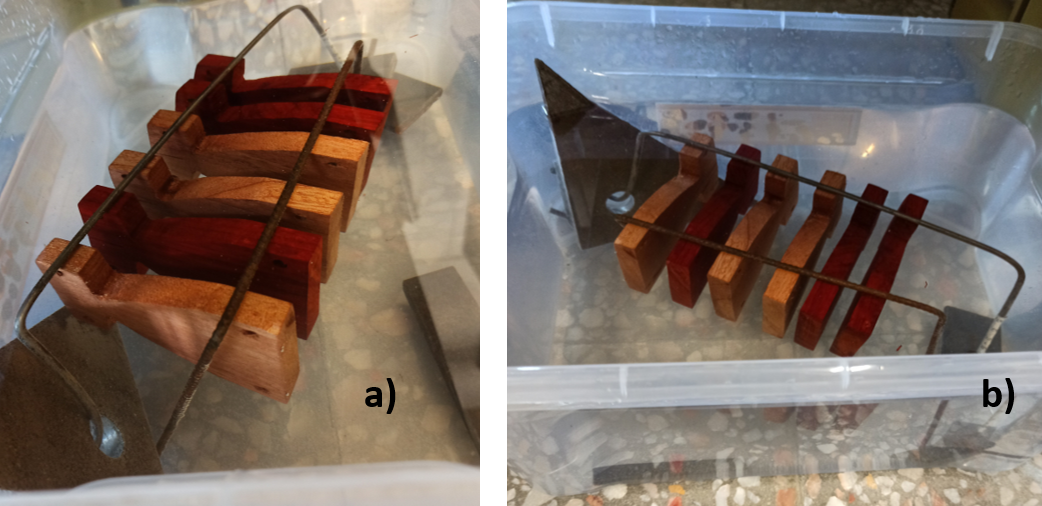
\includegraphics[width=\textwidth]{Figures/WaterSpecimens}
	\caption[Specimen moisture content increase]{Specimen moisture content increase experimental process.}
	\label{fig:Fig13}
\end{figure}

The system was designed in order to prevent the specimens from rising to the surface by flotation. But also, to minimize the specimen surface in contact with the system. Indeed, it allows to maximize the MC rise which take less time to reach the desired MC levels. This fact was verified when all the specimens (from E2 and E3 experiment) were put together into water. Of course, the system was not designed for 12 specimens, and the specimens were really closed. It involves a slower increase of the MC.

After 80.62h as presented in \ref{tab:MC_decrease}, specimens were weighed again. Thanks to these weights, it was possible to plot a shape about, how the MC decreases, and how the weight evolve compared to time. A quick look to the decrease of MC into Okoume specimens show that until 20\% MC, every hour almost 1\% MC is loose. From this value until the ambient MC, the MC decrease process becomes slower as it is shown on \ref{fig:Fig15_b}, with decreasment less than 0.4\% every hour.

Thanks to E3 daily weight, it appears that both species, Okoume and Padouck, earn a constant MC. The difference is the value of this constant increasing. Okoume specimens earn approximately 5\% MC each day, while Padouck ones earn around 2\% MC.

After the first serie of weight, some values were determined.
The purpose is to obtain specimen at a normal temperature, but with a maximum moisture content around 30\%. So by weighting every hour specimens submersed for days, the MC evolution of samples can be expected. One table was created for each specimen as the \ref{tab:MC_decrease} one.

\begin{table}[]
	\centering
	\begin{tabular}{llll}
		\cline{1-2}
		\multicolumn{1}{c}{\cellcolor[HTML]{F8CBAD}E2O1} & \multicolumn{1}{c}{\cellcolor[HTML]{F8CBAD}34,219} & 9,83\% &  \\ \cline{1-2}
		&  &  &  \\ 
		\multicolumn{1}{c}{time} & \multicolumn{1}{c}{Wet Weight} & \multicolumn{1}{c}{MC} & \multicolumn{1}{c}{MC decreasment O1} \\ 
		\multicolumn{1}{l}{\cellcolor[HTML]{A5A5A5}09:13:00} & \multicolumn{1}{l}{67 g} & \multicolumn{1}{l}{95,79765627   \%} &  \\ \cline{1-3}
		\multicolumn{1}{l}{10:22:00} & \multicolumn{1}{l}{66 g} & \multicolumn{1}{l}{92,87530319   \%} &  \\ \cline{1-3}
		\multicolumn{1}{l}{11:22:00} & \multicolumn{1}{l}{65 g} & \multicolumn{1}{l}{89,95295012   \%} &  \\ 
		\multicolumn{1}{l}{12:22:00} & \multicolumn{1}{l}{64 g} & \multicolumn{1}{l}{87,03059704   \%} & \multicolumn{1}{l}{\cellcolor[HTML]{A5A5A5}Day change} \\ 
		\multicolumn{1}{l}{13:22:00} & \multicolumn{1}{l}{63 g} & \multicolumn{1}{l}{84,10824396   \%} & \multicolumn{1}{l}{\cellcolor[HTML]{9BC2E6}Scale change} \\ 
		\multicolumn{1}{l}{14:22:00} & \multicolumn{1}{l}{60 g} & \multicolumn{1}{l}{75,34118472   \%} & \multicolumn{1}{l}{\cellcolor[HTML]{00B0F0}20\% MC reached} \\ 
		\multicolumn{1}{l}{15:22:00} & \multicolumn{1}{l}{60 g} & \multicolumn{1}{l}{75,34118472   \%} & \multicolumn{1}{l}{\cellcolor[HTML]{0070C0}30\% MC reached} \\ 
		\multicolumn{1}{l}{16:35:00} & \multicolumn{1}{l}{59 g} & \multicolumn{1}{l}{72,41883164   \%} & \multicolumn{1}{l}{\cellcolor[HTML]{FFC000}Normal MC reached} \\ 
		\multicolumn{1}{l}{17:43:00} & \multicolumn{1}{l}{59 g} & \multicolumn{1}{l}{72,41883164   \%} &  \\ 
		\multicolumn{1}{l}{18:26:00} & \multicolumn{1}{l}{59 g} & \multicolumn{1}{l}{72,41883164   \%} &  \\ 
		\multicolumn{1}{l}{19:30:00} & \multicolumn{1}{l}{58 g} & \multicolumn{1}{l}{69,49647856   \%} &  \\ 
		\multicolumn{1}{l}{20:37:00} & \multicolumn{1}{l}{56 g} & \multicolumn{1}{l}{63,65177241   \%} &  \\ 
		\multicolumn{1}{l}{21:50:00} & \multicolumn{1}{l}{56 g} & \multicolumn{1}{l}{63,65177241   \%} &  \\ 
		\multicolumn{1}{l}{22:22:00} & \multicolumn{1}{l}{56 g} & \multicolumn{1}{l}{63,65177241   \%} &  \\ 
		\multicolumn{1}{l}{23:05:00} & \multicolumn{1}{l}{55 g} & \multicolumn{1}{l}{60,72941933   \%} &  \\ 
		\multicolumn{1}{l}{00:09:00} & \multicolumn{1}{l}{53 g} & \multicolumn{1}{l}{54,88471317   \%} &  \\ 
		\multicolumn{1}{l}{01:24:00} & \multicolumn{1}{l}{53 g} & \multicolumn{1}{l}{54,88471317   \%} &  \\ 
		\multicolumn{1}{l}{\cellcolor[HTML]{A5A5A5}07:45:00} & \multicolumn{1}{l}{50 g} & \multicolumn{1}{l}{46,11765393   \%} &  \\ 		\multicolumn{1}{l}{09:10:00} & \multicolumn{1}{l}{49 g} & \multicolumn{1}{l}{43,19530086   \%} &  \\ 
		\multicolumn{1}{l}{09:48:00} & \multicolumn{1}{l}{\cellcolor[HTML]{9BC2E6}51,535 g} & \multicolumn{1}{l}{50,60346591   \%} &  \\ 
		\multicolumn{1}{l}{10:49:00} & \multicolumn{1}{l}{51,114 g} & \multicolumn{1}{l}{49,37315526   \%} & \multicolumn{1}{l}{1,230310646 \%} \\ 
		\multicolumn{1}{l}{11:29:00} & \multicolumn{1}{l}{50,737 g} & \multicolumn{1}{l}{48,27142815   \%} & \multicolumn{1}{l}{1,101727111 \%} \\ 
		\multicolumn{1}{l}{12:30:00} & \multicolumn{1}{l}{50,207 g} & \multicolumn{1}{l}{46,72258102   \%} & \multicolumn{1}{l}{1,548847132 \%} \\ 
		\multicolumn{1}{l}{13:45:00} & \multicolumn{1}{l}{49,624 g} & \multicolumn{1}{l}{45,01884918   \%} & \multicolumn{1}{l}{1,703731845 \%} \\ 
		\multicolumn{1}{l}{14:45:00} & \multicolumn{1}{l}{49,225 g} & \multicolumn{1}{l}{43,8528303   \%} & \multicolumn{1}{l}{1,166018878 \%} \\ 
		\multicolumn{1}{l}{15:40:00} & \multicolumn{1}{l}{48,811 g} & \multicolumn{1}{l}{42,64297612   \%} & \multicolumn{1}{l}{1,209854175 \%} \\ 
		\multicolumn{1}{l}{16:36:00} & \multicolumn{1}{l}{48,368 g} & \multicolumn{1}{l}{41,34837371   \%} & \multicolumn{1}{l}{1,294602414 \%} \\ 
		\multicolumn{1}{l}{\cellcolor[HTML]{A5A5A5}09:39:00} & \multicolumn{1}{l}{44,397 g} & \multicolumn{1}{l}{29,74370963   \%} &  \\ 
		\multicolumn{1}{l}{10:34:00} & \multicolumn{1}{l}{43,994 g} & \multicolumn{1}{l}{28,56600134   \%} & \multicolumn{1}{l}{1,177708291 \%} \\ 
		\multicolumn{1}{l}{11:34:00} & \multicolumn{1}{l}{43,612 g} & \multicolumn{1}{l}{27,44966247   \%} & \multicolumn{1}{l}{1,116338876 \%} \\ 
		\multicolumn{1}{l}{13:09:00} & \multicolumn{1}{l}{43,048 g} & \multicolumn{1}{l}{25,80145533   \%} & \multicolumn{1}{l}{1,648207136 \%} \\ 
		\multicolumn{1}{l}{14:26:00} & \multicolumn{1}{l}{42,624 g} & \multicolumn{1}{l}{24,56237763   \%} & \multicolumn{1}{l}{1,239077705 \%} \\ 
		\multicolumn{1}{l}{15:38:00} & \multicolumn{1}{l}{42,279 g} & \multicolumn{1}{l}{23,55416581   \%} & \multicolumn{1}{l}{1,008211812 \%} \\ 
		\multicolumn{1}{l}{16:39:00} & \multicolumn{1}{l}{41,979 g} & \multicolumn{1}{l}{22,67745989   \%} & \multicolumn{1}{l}{0,876705924 \%} \\ 
		\multicolumn{1}{l}{18:44:00} & \multicolumn{1}{l}{41,444 g} & \multicolumn{1}{l}{21,11400099   \%} &  \\ 
		\multicolumn{1}{l}{19:34:00} & \multicolumn{1}{l}{41,323 g} & \multicolumn{1}{l}{20,76039627   \%} & \multicolumn{1}{l}{0,353604723 \%} \\ 
		\multicolumn{1}{l}{\cellcolor[HTML]{A5A5A5}09:22:00} & \multicolumn{1}{l}{39,327 g} & \multicolumn{1}{l}{14,92737953   \%} &  \\ 
		\multicolumn{1}{l}{10:35:00} & \multicolumn{1}{l}{39,196 g} & \multicolumn{1}{l}{14,54455127   \%} & \multicolumn{1}{l}{0,382828253 \%} \\ 
		\multicolumn{1}{l}{11:32:00} & \multicolumn{1}{l}{39,098 g} & \multicolumn{1}{l}{14,25816067   \%} & \multicolumn{1}{l}{0,286390602 \%} \\ 
		\multicolumn{1}{l}{13:12:00} & \multicolumn{1}{l}{38,931 g} & \multicolumn{1}{l}{13,77012771   \%} & \multicolumn{1}{l}{0,488032964 \%} \\ 
		\multicolumn{1}{l}{14:12:00} & \multicolumn{1}{l}{38,833 g} & \multicolumn{1}{l}{13,48373711   \%} & \multicolumn{1}{l}{0,286390602 \%} \\ 
		\multicolumn{1}{l}{15:14:00} & \multicolumn{1}{l}{38,768 g} & \multicolumn{1}{l}{13,29378416   \%} & \multicolumn{1}{l}{0,18995295 \%} \\ 
		\multicolumn{1}{l}{16:06:00} & \multicolumn{1}{l}{38,702 g} & \multicolumn{1}{l}{13,10090885   \%} & \multicolumn{1}{l}{0,192875303 \%} \\ 
		\multicolumn{1}{l}{17:00:00} & \multicolumn{1}{l}{38,652 g} & \multicolumn{1}{l}{12,9547912   \%} & \multicolumn{1}{l}{0,146117654 \%} \\ 
	\end{tabular}
	\caption{Moisture Content and weight decrease depending on time with the E2O1 specimen example}
	\label{tab:MC_decrease}
\end{table}

It is important to notice that the scale change, from a normal one to a really precise one, did not allow to obtain a good curve shape during the first day of weight, as visible on \ref{fig:Fig15_a} and \ref{fig:Fig15_c}. Indeed, \ref{tab:MC_decrease} first values have a gram precision and the scale had a strange behavior. This is also why, the MC decrease on \ref{fig:Fig15_b} and \ref{fig:Fig15_d} was not calculated during these first days. 
\begin{figure}[th]
	\centering
	\begin{subfigure}{0.48\linewidth}
		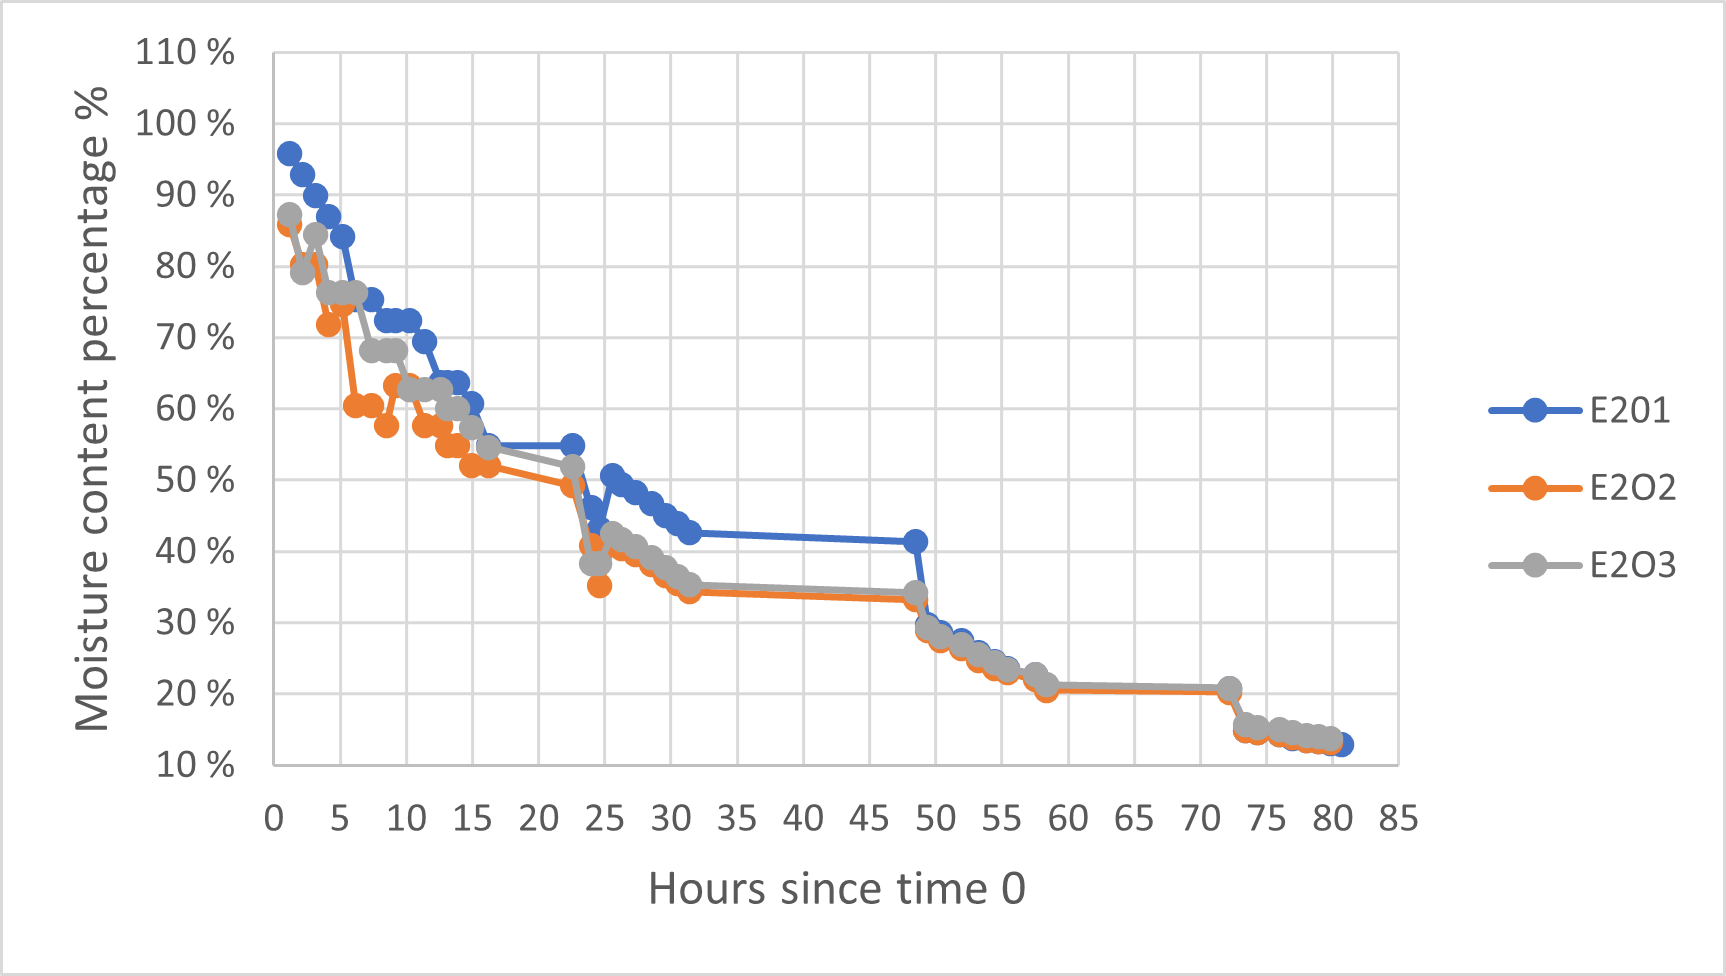
\includegraphics[width=\textwidth]{Figures/Okoume_MCdecreas}
		\caption[Okoume MC decrease depending on time.]{Plot of 3 Okoume specimens MC decrease depending on time.}
		\label{fig:Fig15_a}
	\end{subfigure}
	\hfill
	\begin{subfigure}{0.48\linewidth}
		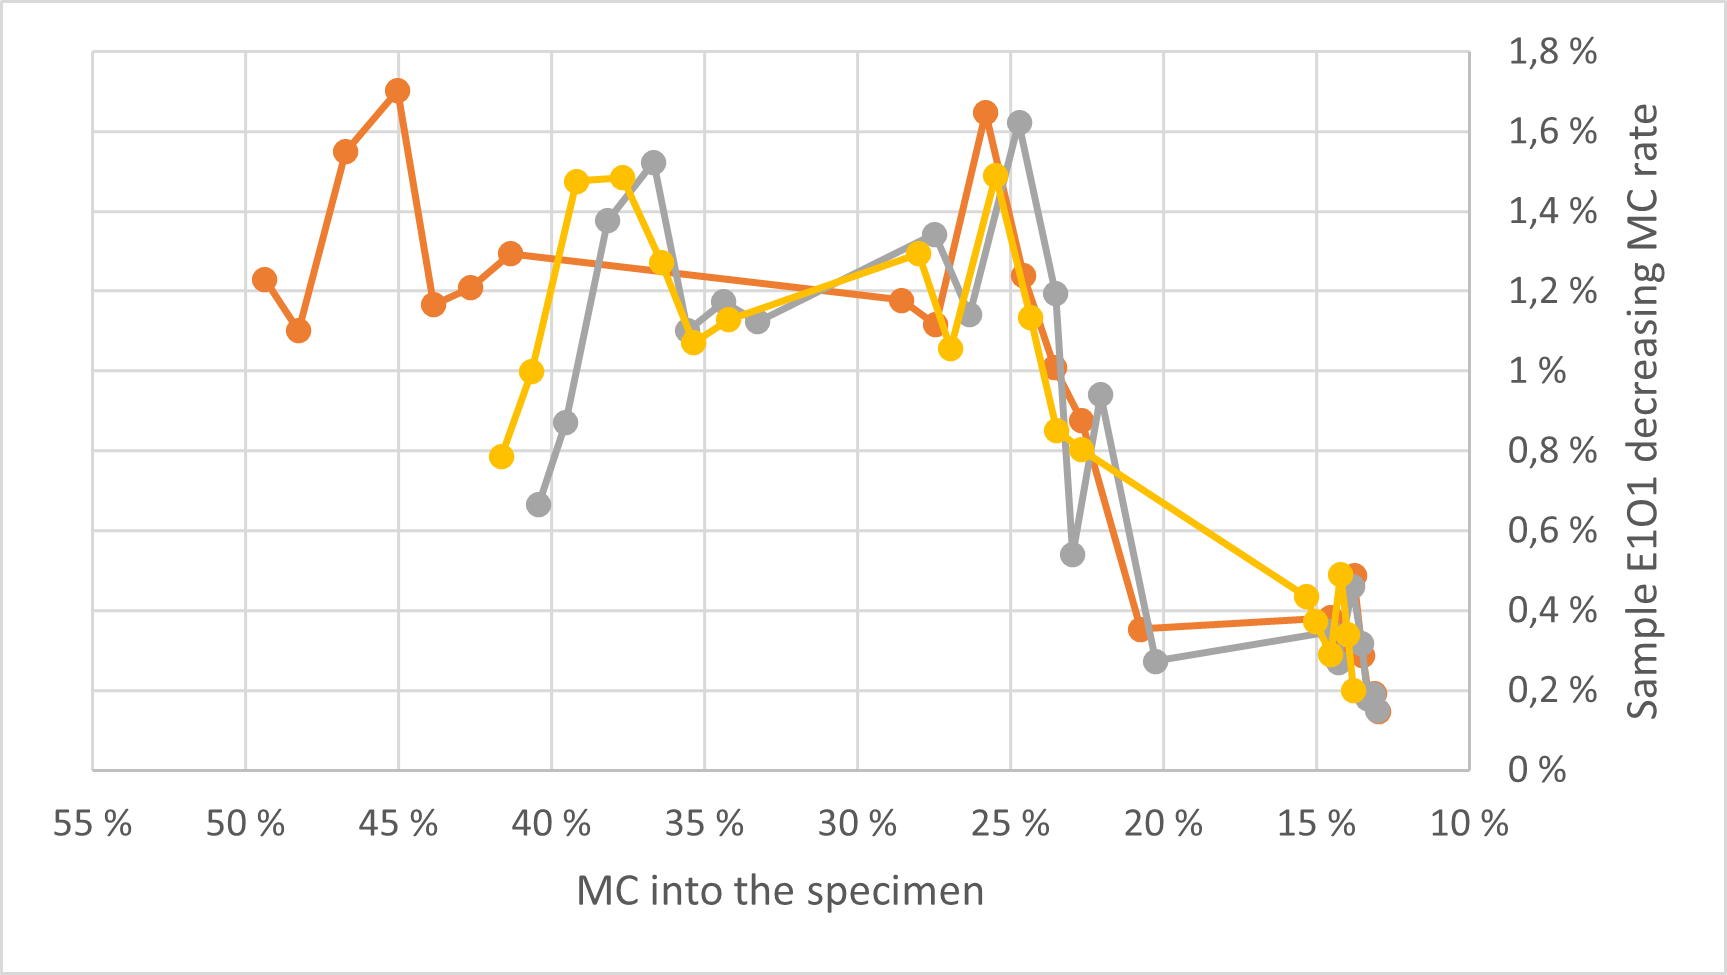
\includegraphics[width=\textwidth]{Figures/Okoume_MCevol}
		\caption[MC decreassement depending on MC for 3 Okoume samples]{Plot of 3 Okoume specimens MC decreassement depending on MC}
		\label{fig:Fig15_b}
	\end{subfigure}
		\hfill
	\begin{subfigure}{0.48\linewidth}
		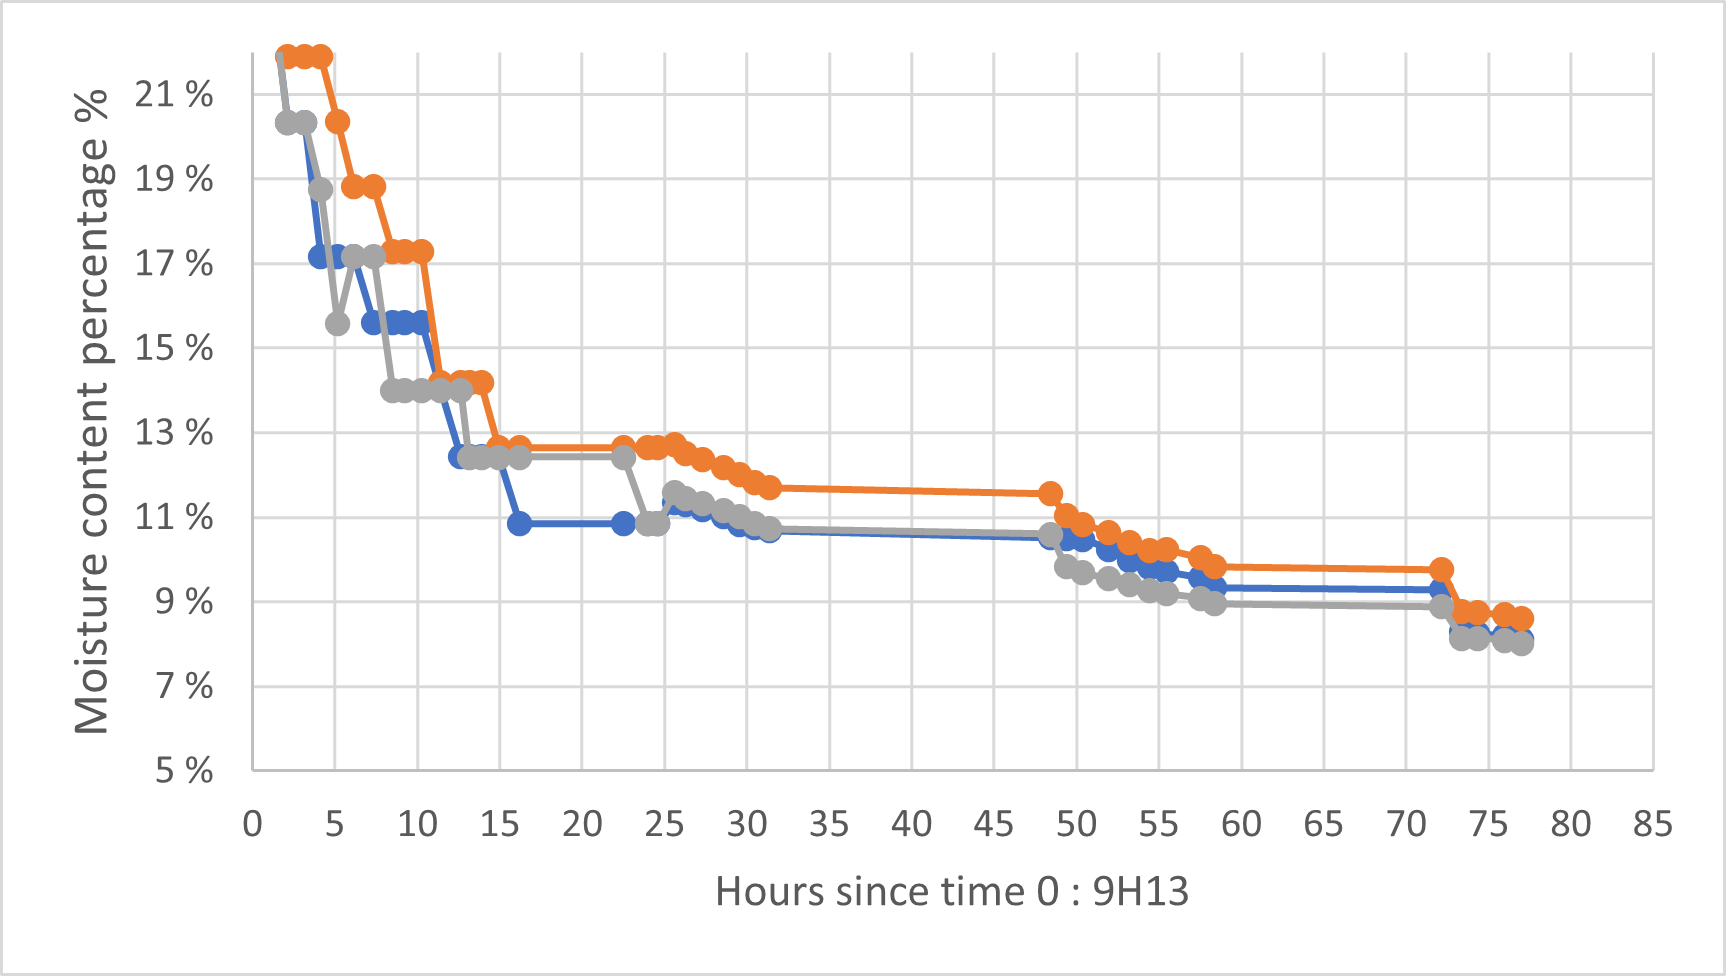
\includegraphics[width=\textwidth]{Figures/Padouck_MCdecreas}
		\caption[Padouck MC decrease depending on time.]{Plot of 3 Padouck specimens MC decrease depending on time.}
		\label{fig:Fig15_c}
	\end{subfigure}
		\hfill
	\begin{subfigure}{0.48\linewidth}
		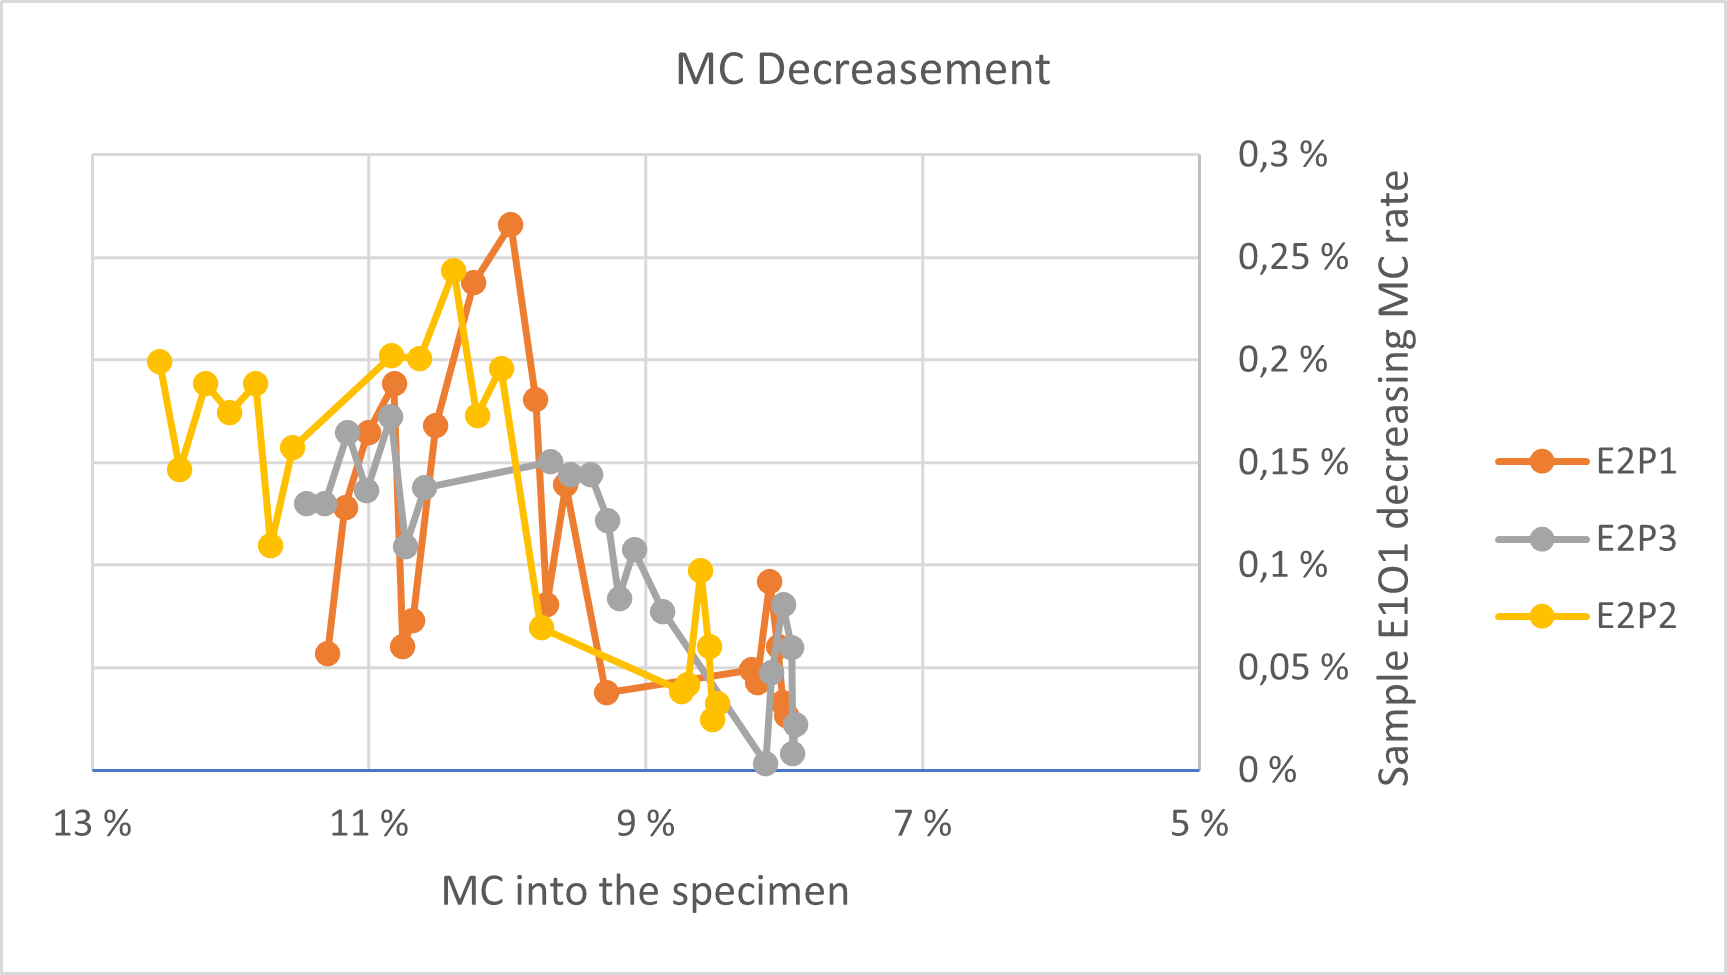
\includegraphics[width=\textwidth]{Figures/Padouck_MCevol}
		\caption[MC decreassement depending on MC for 3 Padouck samples]{Plot of 3 Padouck specimens MC decreassement depending on MC}
		\label{fig:Fig15_d}
	\end{subfigure}
	\caption{MC evolution of specimens}
	\label{fig:Fig15}
	
\end{figure}

Unfortunately, the two important steps, at 20\% and 30\% were reached at a time when the measurement were not done every hour as it is visible on \ref{fig:Fig15_a} or \ref{fig:Fig15_c}. But it allows to have the shape of the curve, showing how the MC decreases depending on time. Thanks to these curves, it was possible to predict, regarding the hours at which the specimens were put off the water, when they must be tested to have the approximate MC expected.

But wood is a living material with a really particular behavior. Looking to this previous parameters, visible in \ref{fig:Fig15_a} and \ref{fig:Fig15_b} an approximation was made. By putting out of the water the specimens at a given hour, they will be tested at a given other. By processing this way, a lot of the experiments were sceduled for 53h after putting them off the water. But in 7 hours Okoume specimen loose around 20\% of MC and Padouck around 7\%. Which is following the previous curve, but for Padouck specimen it was quicker than expected.

%----------------------------------------------------------------------------------------
%	SUBSECTION 3
%----------------------------------------------------------------------------------------

\subsection{Chosen experiments}

Due to the delay and the material made available, some tests could not be done. It was chosen to only study the evolution of energy release rate by the variation of MC. To have more data and create a smoother curve of results, the specimens expected to be tested at different temperature were put into water to increase their MC and have values at a different MC than the average of 20\% and 30\%. It must be noted that, at the contrary of samples scheduled to be tested at different MC, E4 and E5 specimens were put off the water during the morning and tested during the afternoon. They were more wet, so a different behavior was expected.In the same time, Silver Fir specimens were sent from France, to be tested and compared as intended first. Unfortunately, they were waited too long and it was impossible to put them into water in order to obtain results as the same MC as the others species. Therefore, they never arrived and this work is focused on Padouck and Okoume species tested at room humidity, and at 20\%, 30\% MC.

%%%%%%%%%%%%%%%%%%%%%%%%%%%%%%%%%%%%%%%%%%%%%%%%%%%%%%%%%%%
%%%%%%%%%%%%%%%%%%%%%%%%%%%%%%%%%%%%%%%%%%%%%%%%%%%%%%%%%%%


%
%\section{Mode I fracture loading test using the MMCG specimen: data reduction}
%
%\section{Python Code to analysed datas}
%
%\begin{lstlisting}[language=Python]
%import numpy as np
%
%def incmatrix(genl1,genl2):
%    m = len(genl1)
%    n = len(genl2)
%    M = None #to become the incidence matrix
%    VT = np.zeros((n*m,1), int)  #dummy variable
%
%    #compute the bitwise xor matrix
%    M1 = bitxormatrix(genl1)
%    M2 = np.triu(bitxormatrix(genl2),1)
%
%    for i in range(m-1):
%        for j in range(i+1, m):
%            [r,c] = np.where(M2 == M1[i,j])
%            for k in range(len(r)):
%                VT[(i)*n + r[k]] = 1;
%                VT[(i)*n + c[k]] = 1;
%                VT[(j)*n + r[k]] = 1;
%                VT[(j)*n + c[k]] = 1;
%
%                if M is None:
%                    M = np.copy(VT)
%                else:
%                    M = np.concatenate((M, VT), 1)
%
%                VT = np.zeros((n*m,1), int)
%
%    return M
%\end{lstlisting}
%
%\lstinputlisting[language=Python, firstline=180, lastline=202]{Figures/pyMMCG.py}
%

%
%Then, 
%
% :::::::::::::::::::::::::::::::::::::::::::::::::::::
%
%
%

%% Chapter Template

\chapter{Python Reshape}
\label{Python Reshape}

\section{Python program}

%----------------------------------------------------------------------------------------
%	SUBSECTION 1
%----------------------------------------------------------------------------------------

\subsection{Initialization and input values}

The Python code developed is inspired from a previous one, done in MatLab by \parencite{Reference14} for DCB tests. MMCG specimen was created from DCB one, so it was logical to use this program with an adaptation to Python tools. 

The main purpose of this tool is to compute all the information given by DIC and obtain the energy release rate. To do that, it was remind in \ref{eq:Energy release rate equation} that many parameters must be input. Some of them are constant and was measured before or after the test. It is the case for $a_{0}$ and "b" parameters, respectively the initial crack length and the thickness of the specimen analysed. It is dfined in four big parts.

So a first program, allowing to combine all the constants by creating a structure as the one below, was done. It is called database and the following one is the example from the third Okoume specimen of the first experiment database:
\lstinputlisting[language=Python, firstline=1, lastline=9]{Codes/Database.py}

\begin{lstlisting}[language=Python]
	LX, H = 29.3, 1624  # mm / pixel
	if Job == 'e1o3':
	##########################################################################
	# pixel to mm magnification factor
	Test.mm2pixel = LX / H
	# Load conversion factor - testing machine
	Test.LoadConvFactor = 1000  # from kN to N
	# Displacement conversion factor - testing machine
	Test.DisplConvFactor = 2.0  # mm/V (gain = 20 mm)
	Test.thickness = 14 # unit  mm
	Test.a0 = 24.5 # unit  mm
\end{lstlisting}


\lstinputlisting[language=Python, firstline=11, lastline=19]{Codes/Database.py}

Thanks to this database file, open in the main code file, many calls can be done and allow to synthesize the main code. Of course one database was created for each specimen andinput in a single folder, due to the difference between values as the precrack length or the thickness of the specimen. Other values as the "Test.LoadConvFactor" will always be the same. Indeed, in this work, the load values, given by MTS press \ref{fig:Fig8} are given in \si{\kilo\newton}, so a coefficient of 1000 must be added to obtain coherants results.

All the values from MatchID must be read and the displacement or load from the Hydraulic Press have to been stored in Python variables. 

\begin{lstlisting}[language=Python]
# determining the number of stages by inspecting MatchID processing files
stages = glob.glob(os.path.join(cwd, 'DCB_002_*.tif.dat'))
MatchID.stages = stages.__len__()
print('Number of stages: ', str(MatchID.stages))
\end{lstlisting}

The first step is to store in a parameter, the number of stages by looking to the number of images captured by MatchID. As it is visible, variables are created, in a structure named MatchID. Here, the number of stages is stored in MatchID.stages variable. This MatchID structure is present in the database, because it is linked to each specimen. Indeed, the number of images changes from one test to another. So another part of the database is linked to MatchID settings and add information linked to this structure:  

\begin{lstlisting}[language=Python]
	# Summary of DIC Settings
MatchID.CorrelationCoef = 'ZNSSD'
MatchID.InterpolationOrder = 'Bicubic spline'
MatchID.TransformationOrder = 'Affine'
MatchID.Subset, MatchID.Step = 15, 13
# Summary of Strain Settings
MatchID.StrainWindow = 5
MatchID.StrainConvention = 'GreenLagrange'
MatchID.StrainInterpolation = 'Q4'
# Area of Interest
MatchID.Roi_PolyXi, MatchID.Roi_PolyYi = 52, 259
MatchID.Roi_PolyXf, MatchID.Roi_PolyYf = 1587, 1119
\end{customFrame}

It is possible to use thanks to this part, the type of subset used, the steps, the strain window and intrpolation, previously chosen looking on the best parameters on MatchID curves. Then, the displacements and load of every stages must be stored to. In order to do it, an iterative loop is created :

\begin{lstlisting}[language=Python]
# U displacement
UX = np.zeros((MatchID.SubsetsY, MatchID.SubsetsX, MatchID.stages))
tic()
for i in np.arange(0, MatchID.stages, 1):
readstr = #Name of the test
print('reading : ',readstr)
pathdados = os.path.join(cwd,'u',readstr)
aux = np.genfromtxt(pathdados, skip_header=0, delimiter=';')
UX[:, :, i] = aux[:, :-1]*Test.mm2pixel # unit: mm
print(f'{toc():.1f} seg')
\end{lstlisting}

This loop stores the displacement on U direction, but an other similar one do the same on V direction. Ux is a Matrix filled by the reading of MatchID.subset file and the number of stages. Then it is multiply by the convector factor from \si{\pixel} to \si{\milli\meter}. 

%----------------------------------------------------------------------------------------
%	SUBSECTION 3
%----------------------------------------------------------------------------------------

\subsection{Determination of the CTOD} 

After computing all the datas from the database, a second part is computed. It is linked to the Crack Tip Opening Displacement (CTOD). Indeed, this factor has impact on the cohesive law. MatchID is a great tool which does some work for the user. That is why, some of the information from the software program were put in the Database, as in the next code with the ZOI dimensions: 
\begin{lstlisting}[language=Python]
# Allied Manta G-505B
H, V  = 2448, 2050 # unit: pixels
# 'TC2336' telecentric lens
LX, LY = 34.98, 29.18 # unit: mm
\end{lstlisting}

Then, two matrix are created. There are first, declared and made of zeros :

\begin{lstlisting}[language=Python]
CTODI  = np.zeros((ud_lim, 3, MatchID.stages))
# Vup, Vdown, ||Vup-Vdown||
CTODII = np.zeros((ud_lim, 3, MatchID.stages))
\end{lstlisting}

As shown in the code, the dimensions of the matrix take in account the number of stages, so the number of images. Indeed, the interest of the CTOD is to be folowed at each stage. 

Then, a loop is created, allowing to put information into others vectors

\begin{lstlisting}[language=Python]
for J in np.arange(0, MatchID.stages, 1):
# mode I:
uYtemp = np.copy(UY[:, :, J])
CTODI[:, 0, J] = np.flipud(uYtemp[a0.Y - ud_lim: a0.Y, a0.X])
CTODI[:, 1, J] = uYtemp[a0.Y: a0.Y + ud_lim, a0.X]
CTODI[:, 2, J] = np.abs(CTODI[:, 1, J] - CTODI[:, 0, J])
\end{lstlisting}

An other one is also created to compared to mode II values. In the current case, the mode II can be approximate around zero, because it is a mode I test. Then all the values are obtained, for each COD pair until ud$_$lim which is in this case equal to 10. By looking to this different curves, the chosen COD pair is chosen and a curve is plot looking to the values for this parameter chosen by the user. 

\begin{figure}[h]
	\centering
	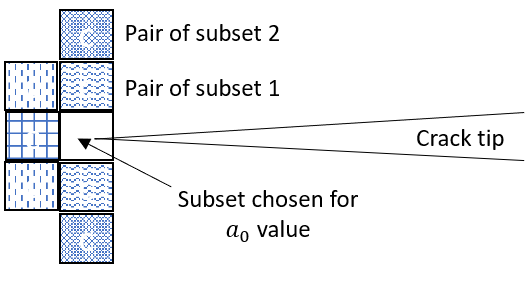
\includegraphics[scale=0.7]{Figures/Subset_choice}
	\decoRule
	\caption[Subset choice and pair of subset around]{Pair of subset around the $a_{0}$ subest chosen}
	\label{fig:subest_chosen}
\end{figure}

Finally, the way to obtain CTOD, alos need a well $a_{0}$ choice. Indeed, the chosen subset as presented on \ref{fig:subest_chosen}, will be determinant. Considering the image as a matrix composed of subset, the chosen subset as a position given by his m row and n column. To determinate the opening, it is necessary to have a look on the subsets in the same n column but at a different line. Indeed, the chosen subset will be the first one affected by the crack, that means, that information on the subset will not have importance anymore. While, looking to subset up and down allow to follow the displacement of the crack tip and measure it. The fact is to determine which pair of subsets is the best. The ones at the row n-1 and n+1, but maybe these ones will be on the crack at a given stage and will lose all the necessary information. That is why, an important choice must be done. Here COD pair was fixed equal to two. So the subset displacement analysed is the one of the pair of subset 2 on \ref{fig:subest_chosen}. Finally, by looking to these displacements, it is possible to obtain the value of the crack opening at each stages.

%----------------------------------------------------------------------------------------
%	SUBSECTION 4
%----------------------------------------------------------------------------------------

\subsection{Crack length analysis}

The third part of the code has the purpose to determine a(t), so the crack length evolution. This evolution can be compared to the time or the hydraulic press dispacement and also the load applied on the specimen. The first step is again to define everything. The displacement are stored again, the Zone Of Interest (ZOI) is defined by supressing the value out of this ZOI.
This a(t) parameter is the most difficult to obtain, indeed tools as MatchID cannot help the user to obtain the result stage by stage. The value of a(t) will be equal to $a_{0}$ fixed by the user and add to a $\Delta a$ which is the value of the crack length, evolving in time due to the applied force.

\begin{lstlisting}[language=Python]
displ_x = UX[:,:,J]
displ_y = UY[:,:,J]
# resize RoI containing the crack growth process
if roi == 'crop':
displ_x = displ_x[Y_i:Y_f,X_i:X_f]
displ_y = displ_y[Y_i:Y_f,X_i:X_f]

# find the dimensions of the matrix
m = displ_x.shape[0] #  y - row
n = displ_x.shape[1] # x - column
# find the matrix with the displacements
displ = (displ_x**2 + displ_y**2)**0.5
# preallocation: zeros
n_zeros = np.zeros((m, 1))
m_zeros = np.zeros((1, n+1))
\end{lstlisting}

After defining all the parameters, the displacement of the crack tip is observed thanks to some calculus on the subsets. 

\begin{lstlisting}[language=Python]
displ_A = np.vstack((np.hstack((displ,n_zeros)), m_zeros))/4
# divided by 4 because sum: displ_A+displ_B+displ_C+displ_D
displ_B = np.vstack((np.hstack((n_zeros,displ)), m_zeros))/4
displ_C = np.vstack((m_zeros, (np.hstack((displ, n_zeros)))))/4
displ_D = np.vstack((m_zeros, (np.hstack((n_zeros, displ)))))/4
# auxiliar matrix 2 edges; 4 within the matrix 'matr_transf'
matr_transf = np.ones((m+1, n+1))
matr_transf[:, 0] = 2
matr_transf[:, -1] = 2
matr_transf[0, :] = 2
matr_transf[-1, :] = 2
matr_transf[0, 0] = 4
matr_transf[0, -1] = 4
matr_transf[-1, 0] = 4
matr_transf[-1, -1] = 4
grid_values = (displ_A + displ_B + displ_C + displ_D)*matr_transf
# displacements of each corner on the facet
displ_A = grid_values[0:-1, 0:-1]
displ_B = grid_values[0:-1, 1:]
displ_C = grid_values[1:, 0:-1]
displ_D = grid_values[1:, 1:]
# oblique distance between facet centroids
displ_CA = np.abs(displ_C-displ_A)
displ_DB = np.abs(displ_D-displ_B)
# auxiliar function for the crack tip location criterion
K = np.maximum(displ_CA, displ_DB)
avgK = np.nanmean(K) #mean ignoring nan values.
stdK = np.nanstd(K)
maxK = np.nanmax(K)
if maxK < avgK + inb*stdK:
J = J + 1
else:
JJ = 0
\end{lstlisting}

Here, all the matrix, composed of the subsets from the Zone of Interest are changed by the different steps shown overhead. All the subsets are considered four by four and operatins are done on them. The displacement from one compared to it neighbor are computed. Then average and maximum values are obtained for each subsets of the ZOI and put into K matrix. By using the $a_{0}$ data and looking to the alpha parameter, permitting to compute the best shape of a(t), having the more precise values but numerous ones also, a(t) is obtained with a similar methode. It must be noticed, that to determinate a(t) parameter, $\alpha$ parameter is needed. This one is used on matrix as the M matrix. Indeed, M matrix represents, for a given stage, the crack length by having bigger value in the crack area as shown on \ref{fig:Fig11} : 

\begin{figure}[h]
	\centering
	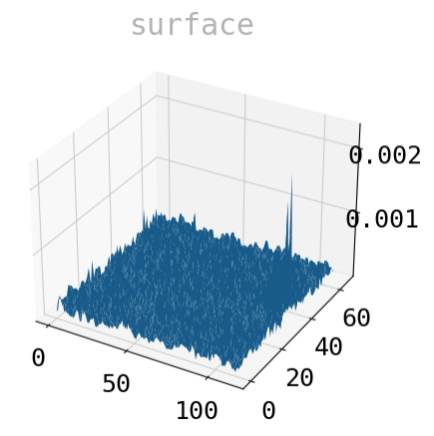
\includegraphics[scale=0.5]{Figures/M_matrix}
	\decoRule
	\caption[M matrix]{M matrix, obtained by running python code}
	\label{fig:Fig11}
\end{figure}

As it is visible, if the user is looking too close, the noise of the values will avoid a good analyze, but by looking too high on the matrix, the crack length value will not be accurate. To move and have a precise idea of the way the user can watch the M matrix, it is important to use $\alpha$. Alpha parameter is like a cutting tool which allows to be as close as the noise without troubles.
To approximate the $\alpha$ value, a correlation factor is searched by least square regression method. The objective it to have the best linear part. A plot is created to show which stage is the most appropriate as on \ref{fig:Fig12}.

\begin{lstlisting}[language=Python]
	### 2 criterion for checking stage
	####
	inb = 3
	# standard deviation * inb (to be checked by user)
	# inb = 1: 68.3 %
	# inb = 2: 95.4 %
	# inb = 3: 99.7 %
\end{lstlisting}

It is possible to adapt the alpha parameter precision by choosing a different "inb" as presented in the code overhead. Indeed, the correlation factor change depending on this criterion. The chosen stage is the one, before the beginning of the crack propagation, but the nearest to the expansion of a(t) length.

\begin{figure}[h]
	\centering
	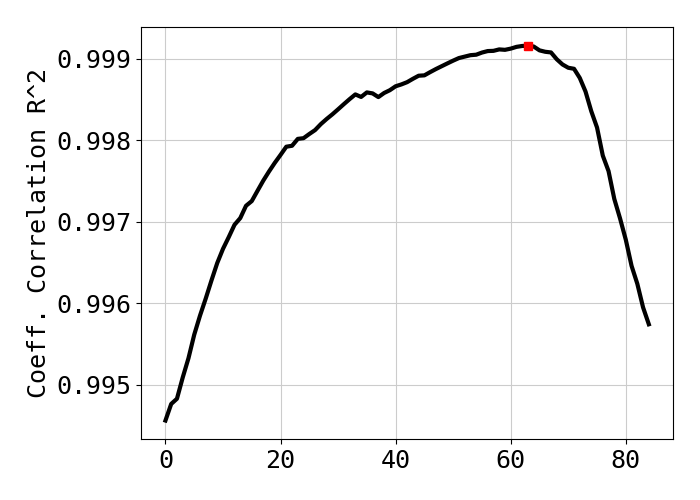
\includegraphics[scale=0.3]{Figures/Correlation_factor}
	\decoRule
	\caption[R correlation factor]{R correlation factor allowing to know which load and disalcement is linked to crack beggining.}
	\label{fig:Fig12}
\end{figure}

This method was the one used by \parencite{Reference14} on MatLab, and have already prooved a good functionnement.

%%----------------------------------------------------------------------------------------
%%	SUBSECTION 5
%%----------------------------------------------------------------------------------------
\subsection{Compliance and Energy values}

The last part of the code consists in using all the calculated parameters, in order to obtain the energy release rate. It is done by computin the G formula as presented below.

\begin{equation}
	G_{c}= \frac{F_{c}^2}{2b} (\frac{\Delta C}{\Delta a})_{d} 	
	\label{eq:Energy release rate equation}
\end{equation}

This equation already given, is written on Python as :

\begin{lstlisting}[language=Python]
a_t = crackL_J_mm[:,chos_alp]

C = MatchID.displ/MatchID.load

# P**2/2/B* dC / da
ALP = (MatchID.load**2)/(2*Test.thickness)

# C = MatchID.displ/MatchID.load

# BET = C/a_t #changing the value of alpha from the crack length will change G values
#
G = ALP*BET
# G = np.dot(ALP,BET)
\end{lstlisting}

In this case, the formula used, is the simplest one, which allow to easily obtain C by dividing the displacement from hydraulic press by the load. These values are stored in MatchID variable, allowing to synthesize all the datas in one per image (stage). An average are done on the seven values between two images. This fact can also involve a little mistake.
Therefore, as explained in "alpha" and "a(t) determination" sections, the crack length depends on alpha parameter. So some curves are ploted depending on "a(t)" matrix changes according to the alpha. The best R-curves must be determined for the most precise crack length. So it is necessary to find a great alpha parameter to have these final values without huge mistake.

\begin{lstlisting}[language=Python]
# write array results on a csv file:
RES = np.array([MatchID.displ[:], MatchID.load[:], C[:], COD.wI[:], a_t[:], G[:]])
RES = np.transpose(RES)
\end{lstlisting}

At least, values as the displacement, the load, the compliance, the CTOD, the crack length and the energy release rate, are stored into a matrix and then exported to .csv files. It allows to save datas, but also to compute everytthing in Excel in addition to python processing tool.

Many improvements are made on the Python code, even after this work ended. Indeed, it apears that the crack length can be better compute, in order to avoid some strange shapes of R-curves. But using the same tool for all specimens computation, even if mistakes exist, it is possible to compare datas.

%%%%%%%%%%%%%%%%%%%%%%%%%%%%%%%%%%%%%%%%%%%%%%%%%%%%%%%%%%%%%
%%%%%%%%%%%%%%%%%%%%%%%%%%%%%%%%%%%%%%%%%%%%%%%%%%%%%%%%%%%%%
%%%%%%%%%%%%%%%%%%%%%%%%%%%%%%%%%%%%%%%%%%%%%%%%%%%%%%%%%%%%%

%
%\subsection{Alpha parameter}
%
%To begin with, it is important   to determinate a parameter, that we had called $\alpha$. This one is used on matrix as the M matrix. Indeed, M matrix represents, for a given stage, the crack length by having bigger value in the crack area as shown on \ref{fig:Fig11} :
%
%\begin{figure}[h]
%	\centering
%	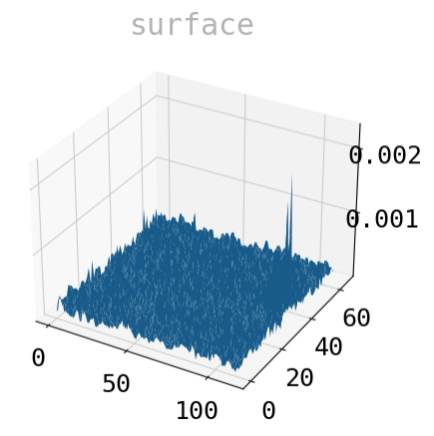
\includegraphics[scale=0.5]{Figures/M_matrix}
%	\decoRule
%	\caption[M matrix]{M matrix, obtained by running python code}
%	\label{fig:Fig11}
%\end{figure}
%As it is visible, if the user is looking too close, the noise of the values will avoid a good analyze, but by looking too high on the matrix, the crack length value will not be accurate. To move and have a precise idea of the way the user can watch the M matrix, it is important to use $\alpha$. Alpha parameter is like a cutting tool which allow to be as close as the noise without troubles.
%To approximate the $\alpha$ value, a correlation factor is searched by least square regression method. The objective it to have the best linear part.
%\begin{customFrame}
%	#### alpha evaluation
%	### Selecting stage for investigating alpha
%	####
%	# least-squares linear regression
%	porder = 1
%	xx = Test.disp # displacement (mm)
%	yy = Test.load # load (N)
%	# Data point in the linear least-squares regression
%	limsup = int(0.75*np.argwhere(max(yy)==yy)[-1])
%	# number of maximum data points for LSR
%	liminf = int(np.round((1/3)*limsup))# number of minimum data points for LSR
%	
%	xx, yy = xx[0:limsup], yy[0:limsup]
%	Rtot = np.zeros((limsup-liminf,1))
%	C_M = np.zeros((limsup-liminf,1))
%	for j in np.arange(0,limsup-liminf,1):
%	limt_sup = liminf + j
%	xfit, yfit = xx[0:limt_sup], yy[0:limt_sup]
%	p  = np.polyfit(xfit, yfit, porder)
%	C_M[j] = 1/p[0]
%	dev = yfit - np.mean(yfit) # deviations - measure of spread
%	SST = np.sum(dev**2) # total variation to be accounted for
%	resid = yfit - np.polyval(p, xfit) # residuals - measure of mismatch
%	SSE = np.sum(resid**2) # variation NOT accounted for
%	Rtot[j] = 1 - SSE/SST #  variation NOT accounted for
%	
%	# position for the best fitting point parameters
%	jmax = np.max(np.argwhere(np.max(Rtot)==Rtot))
%	J = int(liminf + jmax)
%	
%	### 2 criterion for checking stage
%	####
%	inb = 3
%	# standard deviation * inb (to be checked by user)
%	# inb = 1: 68.3 %
%	# inb = 2: 95.4 %
%	# inb = 3: 99.7 %
%	JJ = 1
%	while JJ == 1:
%\end{customFrame}
%
%\begin{figure}[h]
%	\centering
%	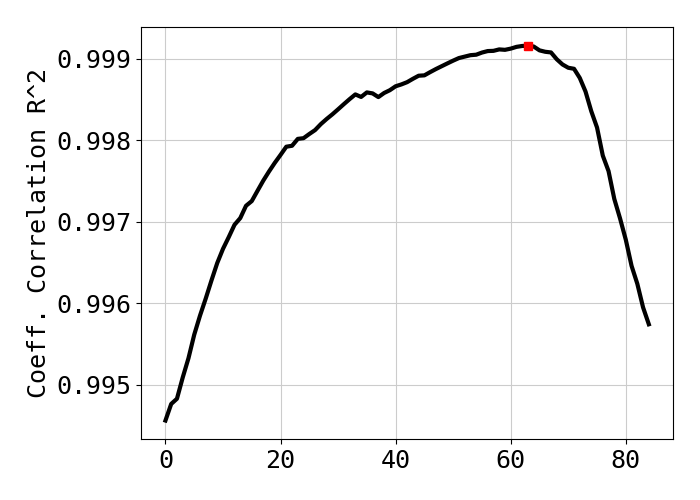
\includegraphics[scale=0.3]{Figures/Correlation_factor}
%	\decoRule
%	\caption[R correlation factor]{R correlation factor allowing to know which load and disalcement is linked to crack beggining.}
%	\label{fig:Fig12}
%\end{figure}
%
%The red dot shown on \ref{fig:Fig12}, is linked to another plot,
%
%Then a matrix representing the subsets in the Area of Interest will be created. First this matrix is composed of zero. Then, the four corners of the matrix will be used to proceed several operations on the matrix. The external lines and columns will take a value of 2 and the corners a value of 4. The distance between opposite corners is calculated and their displacements are compared. Calling K, the maximal displacement of the two corners, average K and maximum one between all the steps are compared. Again, every subset is treated and are still zero when the material is undamaged. It becomes -1 in a region where the material is damaged, and no information are treatables. And it becomes 1 where a discontinuity appears but the wood is not completely damaged like the crack tip. So, by following the farthest 1 value in the matrix, it is possible to know the last subset where the crack tip is localized. Thanks to this distance, some conversions are necessary, from subset to pixel first, and then from pixel to millimeters. Finally, the crack length is determined depending on stages so it could be linked to load or displacement, and thanks to the previous work, to CTOD. The compliance is calculated by dividing the displacement by the load. G is the last variable calculated, with all the previous variables determined, as CTOD presented below and a(t). The last plot is the R-curve representing the Energy release and the crack length.
%%----------------------------------------------------------------------------------------
%%	SUBSECTION 3
%%----------------------------------------------------------------------------------------
%
%\subsection{Determination of the CTOD}
%
%Another partof the code has the purpose to calculate the Crack Tip Opening Displacement (CTOD). MatchID is a great tool which does some work for the user. That is why, by using “wI aramis2D.csv” CTOD is almost find, depending on the time and the load applied. It is important to understand how it works.
%
%First, a part of the work is to define the zone of interest (ZOI), the one where the crack must develop. It is done on MatchID, but also on Python by using the number of the subset defined by Match ID. Then, when a subset is out of this region, it will be considered as equal to zero. Then, the subsets which are placed into the crack, or somewhere where there is a default or missing information as into the crack, the substep will be defined with a value equale to -1. Then, for all the substep around the crack, which have a real interest in the study, they will take the value equal to 1. By using this matrix of substep, now, composed of -1, 0, 1 value, it is possible to plot the entire matrix into grey nuances, and have a look at the crack development, by adding matrix, given by different stages.
%
%\begin{customFrame}
%	ud_lim = 10
%	# Uup, Udown, ||Uup-Udown||
%	CTODI  = np.zeros((ud_lim, 3, MatchID.stages))
%	
%	for J in np.arange(0, MatchID.stages, 1):
%	# mode I:
%	uYtemp = np.copy(UY[:, :, J])
%	CTODI[:, 0, J] = np.flipud(uYtemp[a0.Y - ud_lim: a0.Y, a0.X])
%	CTODI[:, 1, J] = uYtemp[a0.Y: a0.Y + ud_lim, a0.X]
%	CTODI[:, 2, J] = np.abs(CTODI[:, 1, J] - CTODI[:, 0, J])
%	COD.wI = CTODI[COD.cod_pair, 2, :]
%\end{customFrame}
%
%\begin{figure}[h]
%	\centering
%	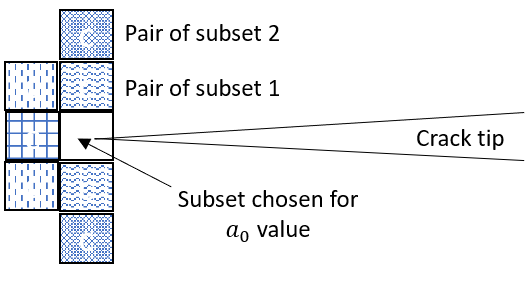
\includegraphics[scale=0.7]{Figures/Subset_choice}
%	\decoRule
%	\caption[Subset choice and pair of subset around]{Pair of subset around the $a_{0}$ subest chosen}
%	\label{fig:subest_chosen}
%\end{figure}
%
%To obtain CTOD, it is important to be careful to $a_{0}$ choice. Indeed, the chosen subset as presented on \ref{fig:subest_chosen}, will be determinant. Considering the image as a matrix composed of subset, the chosen subset as a position given by his m row and n column. To determinate the opening, it is necessary to have a look on the subsets in the same n column but at a different line. Indeed, the chosen subset will be the first one affected by the crack, that means, that information on the subset will not have importance anymore. While, looking to subset up and down allow to follow the displacement of the crack tip and measure it. The fact is to determine which pair of subsets is the best. The ones at the row n-1 and n+1, but maybe these ones will be on the crack at a given stage and will lose all the necessary information. That is why, an important choice must be done. Here COD pair was fixed equal to two. So the subset displacement analysed is the one of the pair of subset 2 on \ref{fig:subest_chosen}. Finally, by looking to these displacements, it is possible to obtain the value of the crack opening at each stages.
%
%%----------------------------------------------------------------------------------------
%%	SUBSECTION 4
%%----------------------------------------------------------------------------------------
%
%\subsection{Crack length analysis}
%
%At least, an important step in this code is the determination of $a_{DIC}$. This parameter is the crack length, which evolves with time during all the experiment. This factor is the most difficult to obtain, indeed tools as MatchID cannot help the user to obtain the result stage by stage. The value of a(t) will be equal to $a_{0}$ fixed by the user and additional to a $\Delta a$ which is the value of the crack length, evolving in time due to the applied force.
%
%\begin{customFrame}
%	roi = 'crop' # 'all'; 'crop'
%	i, incr = 1, 1
%	# incr : is used to step over stages if required (default = 1: all stages)
%	Y_i, Y_f = 0, UY.shape[0]
%	X_i, X_f = 0, a0.X
%\end{customFrame}
%
%\begin{customFrame}
%	# estimation of crack tip length
%	tipstep = np.zeros((alphaint.shape[0],1)) # unit: substep
%	tipmm = np.zeros((alphaint.shape[0],1)) # unit: mm
%	
%	for kk in np.arange(0,alphaint.shape[0],1):
%	alpha = alphaint[kk]
%	# Criterion for crack tip location
%	Kt = np.zeros(K.shape)
%	Kt[np.isnan(K)] = -1
%	Kt[K>=alpha*avgK] = 1
%	Ktemp = Kt
%	# n1 which must be relative to 'a0'
%	ind = np.argwhere(Ktemp==1)
%	row, col = ind[:,0], ind[:,1]
%	if len(col) == 0:
%	tipstep[kk] = 0
%	else:
%	tipstep[kk] = a0.X - np.min(col) # X component
%	# pixel>mm: [macro-pixel*(pixel/macro-pixel)*(mm/pixel)
%	tipmm[kk] = np.abs(tipstep[kk]*MatchID.mm2step - MatchID.mm2step)
%	
%	# for selected  alpha parameters you compute crack length
%	# crack length however should be ZERO at the beginning (no crack propagation)
%	ind = np.where(np.abs(tipmm - np.min(tipmm)) == 0)
%	alpha_alphasel = alphaint[ind[0][0]]
%\end{customFrame}
%A final part of the code allows to obtain a(t) depending on alpha  as it is done on \parencite{Reference14} article. It is done by a focus on the ZOI and the number of subsets composing it. Thanks to the matrix composed by every subsets, the displacement field can be observed. It is obtained by computing the distance between the center of a subset and it displacement from one image to the next one as shown in the literature review. To simplify the code, it is not done on every subset but only on the four corners. By computing the distance between the opposite corners, the maximum x-displacement and an y-displacement are input in a last matrix. 
%
%%----------------------------------------------------------------------------------------
%%	SUBSECTION 5
%%----------------------------------------------------------------------------------------
%
%\subsection{Compliance and Energy values}
%
%As said in alpha parameter section, The last step is to compute the Compliance and then the Energy release rate. Indeed, all the necessary parameters are present in the Python variables. So by computing the formula \ref{eq:Energy release rate equation} the different matrix composed of all the values depending on the stage are used to obtain first a compliance matrix with same dimensions of the CTOD and the dispacement of the Hydraulic press matrix created.
%
%\begin{customFrame}
%	ALP = (Test.load*Test.load)/(2*Test.thickness)
%	print(ALP)
%	
%	C = Test.disp/Test.load
%	
%	BET = C/crackL_J_mm[:,4]
%	
%	G = ALP * BET
%	
%	fig, ax = plt.subplots(figsize=(7,5), dpi=80)
%	plt.plot(crackL_J_mm[:,0], G, 'b-.', linewidth=2, label='R-Curve alpha 1')
%	plt.plot(crackL_J_mm[:,1], G, 'r--', linewidth=2, label='R-Curve alpha 2')
%	plt.plot(crackL_J_mm[:,2], G, 'g-', linewidth=2, label='R-Curve alpha 3')
%	plt.plot(crackL_J_mm[:,3], G, 'k:', linewidth=2, label='R-Curve alpha 4')
%	plt.plot(crackL_J_mm[:,4], G, 'c-.', linewidth=2, label='R-Curve alpha 5')
%	plt.plot(crackL_J_mm[:,5], G, 'm:', linewidth=2, label='R-Curve alpha 6')
%	plt.plot(crackL_J_mm[:,6], G, 'y--', linewidth=2, label='R-Curve alpha 7')
%	plt.xlabel('Crack length, a(t), mm')
%	plt.ylabel('$G_{Ic}, mm$')
%	
%\end{customFrame}
%
%As presented in this part of the code, after calculating G, some plots are created. But as explained in "alpha" and "a determination" sections, the crack length depends on alpha parameter. So some curves are ploted depending on "a" matrix changing according to the alpha.And the best R-curves must be determined for the best crack length. It is necessary to find the best alpha parameter to have these final values.
%
%Finaly, 
\chapter{Experimental work and Result} % Main chapter title
\label{Chapter3} % Change X to a consecutive number; for referencing this chapter elsewhere, use \ref{ChapterX}


%----------------------------------------------------------------------------------------
%	SECTION 1
%----------------------------------------------------------------------------------------
\section{Experimental Setup}


%----------------------------------------------------------------------------------------
%	SUBSECTION 1
%----------------------------------------------------------------------------------------
\subsection{Camera and MatchID Setup}

An Allied Vision Manta 505B 2/3'' camera coupled to an Opto Engineering TC 23 36 telecentric lens were used for image formation and acquisition. The camera is equipped with Charge-Coupled Device (CCD) sensor with pixel resolution of 2452 (H) $\times$ 2056 (V) (5MP) and sensor size of 2/3''. The monovision camera-lense optical system was fixed on a tripod and its spatial position oriented with regard to the target surface of interest. The telecentric lens has a magnification factor of \num{0.243}$\times$, allowed to image a field of view, in the object space, of 36.2$\times$27.1 \si{\milli\meter\squared}. The front of the lens was positioned at a working distance of 103.5 \si{\milli\meter} with an aperture of $f$/8, yielding a field of depth of 11 \si{\milli\meter}.

A high power adjustable ring light was used to illuminate the region of interest. A monochromatic version corresponding to a green wavelength of \num{525} \si{\nano\meter} was used from which the highest spectral response of the camera sensor will be expected.

All the specimens were painted to obtain a speckle pattern suitable for image correlation. A thin layer of white paint was firstly added using a mate spray, followed by a diffuse distribution of black paint to create a unique local pattern across the region of interest at the crack tip (Figure~\ref{fig:Fig17}).

\begin{figure}[t]
	\centering
	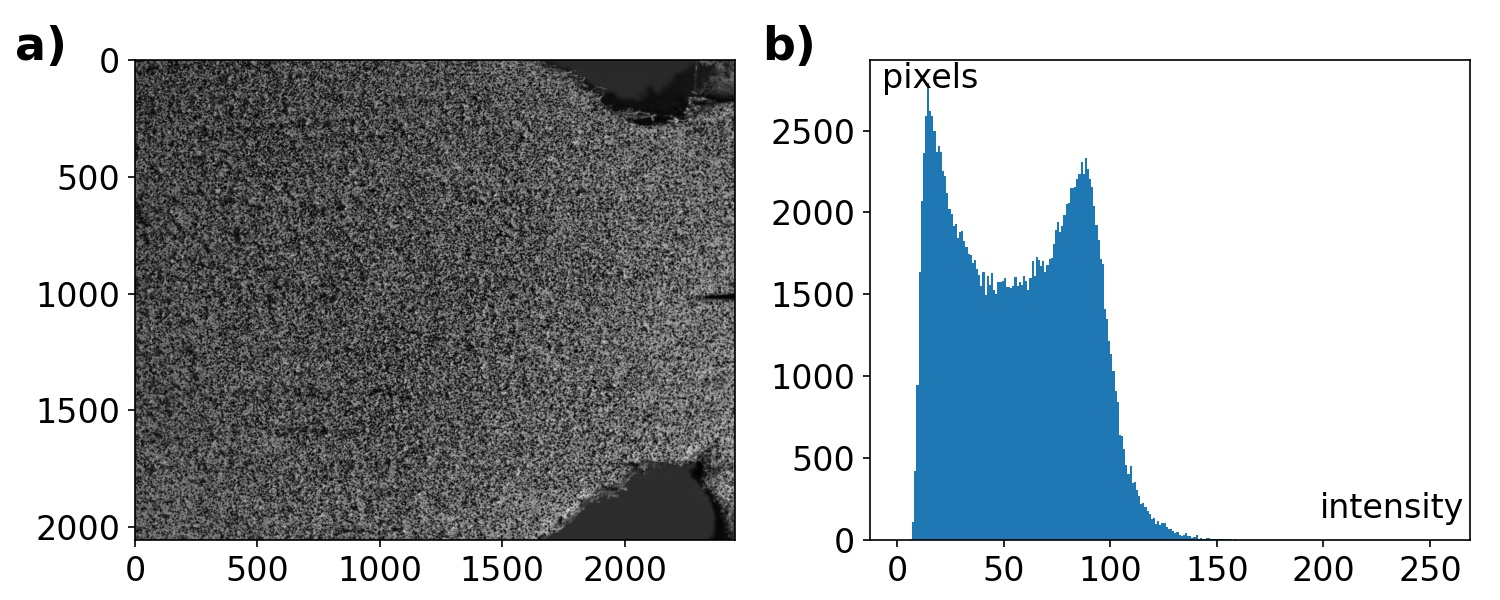
\includegraphics[width=.9\textwidth]{Figures/SpecklePattern}
	\decoRule
	\caption{(a) Speckle pattern typically obtained for DIC measurements (2452 $\times$ 2056
		pixels\textsuperscript{2}); (b) Histogram
		of the
		speckle image
		(256
		gray levels, 8 bits camera).}
	\label{fig:Fig17}
\end{figure}

%\section{DIC measurements and settings}

The DIC setting parameters can have a significant influence on the kinematic fields obtained by image correlation (\textit{e.g.} subset size, subset step, \ldots) and numerical differentiation (\textit{e.g.} strain windows size) algorithms \cite{Pereira2018566}. These settings represent fundamental parameters since they will define the spatial resolution and accuracy associated to the DIC measurements, both in displacement and strain fields.  Therefore, a parametric study was carried out to justify the DIC setting for the current
application, in a balance between resolution and spatial resolution. This study was carried ot in the Parametric Module of MatchID 2D software.
\begin{table}[]
	\centering
	\begin{tabular}{c c}
		\hline
		Correlation   Coefficient: & ZNSSD \\ 
		Interpolation order: & Bicubic Splines \\ 
		Transformation order: & Affine \\
		Subset size: & 21 \\
		Step size: & 5 \\
		Maximum rigid body estimation: & 100 \\ 
		Strain Estimation(\%): & 5 \\ 
		Precision: & 0.001 \\ 
		Maximum iterations: & 20 \\ 
		Noise handling: & Gaussian \\ 
		Kernel Size: & 5 \\ 
		History: & Spatial \\ 
		Strainwindow size: & 7 \\ 
		Tolerance on number of points: & 0 \\ 
		Strain interpolation: & Q4 \\ 
		Strain Convention: & Green-Lagrange \\ \hline
	\end{tabular}
	\caption{MatchID parameters used}
	\label{tab:MatchID_param}
\end{table}
\ref{tab:MatchID_param} defines the range of values defined in this performance analysis which includes the subset size ($f_s$), subset step, affine and quadratic displacement shape functions, the strain windows size and the order of the polynomial fitting function. The pre-selected range of values are deemed to be representative of the range of acceptable DIC setting parameters. For instance, The lower pixel boundary is constrained by aliasing effects, which is a function of the speckle size on the imaged pattern. The subset size defines the target matching pattern used in the correlation algorithm. A rule of thumb will be three contrasted speckles per subset. The average speckle size was determined as 4.5 pixels. Therefore, the minimum subset step was set to 15 pixels. The upper pixel limit can be problem-dependent, taking into account the deformation gradients expected within the region of interest, in a balance between spatial resolution and resolution. As a guideline, larger subsets improves the resolution but decreases spatial resolution. Parameters such as the subset step ($f_p$) (distance between centroids of adjacent subsets, units: pixels) and the strain window $\varepsilon_w$ (number of subsets central points used to define a mesh of data points over which a piecewise polynomial fitting will be applied, using least-square regression, for strain reconstruction) will define a strain spatial resolution ($\Delta \varepsilon$) and virtual strain gauge (VSG), respectively, according to the following relationships \cite{Lava2013576,Pereira2018566}: $\Delta \varepsilon = (\varepsilon_w-1)f_p + f_s$ and $\mbox{VSG} = (\varepsilon_w-1)f_p + 1$ (unit: pixel). For convenience, these parameters can be converted to physical units in the object space (\textit{e.g.} mm), by simple multiplication by the conversion factor of the optical imaging system. All these external DIC parameters, therefore, must be carefully selected in the current study.


A single pair of images, including a reference and deformed image at a force of about 100 N were selected to carry out this study. The obtained results are shown in Figure ?. In this plot the signal of interest, is plotted with regard to a measure of the strain spatial resolution given by the parameter Virtual Strain Gauge (VSG). Both the $y$ component of the displacement and $\varepsilon_{yy}$ component of strain are presented to support the DIC setting selection. Therefore
%----------------------------------------------------------------------------------------
%	SUBSECTION 2
%----------------------------------------------------------------------------------------
\subsection{Servohydraulic test machine and grips Setup}

The servohydraulic test machine, was setup by Mr Martins. The first step was to assembled the grips in the press. They are screwed, for the first one, into one static part of the press, the upper side. The other grip is placed in the moving part. Between every test, the grips must be disassembled and well screwed to maintain each specimen, as well as possible. To change the specimen between two tests, manual command are used to elevate the moving part of the press and avoid the tension in the grips. Of course this pre-tension was also applied on the specimen before the beginning of the test, in order to avoid specimen movement due to the screwed grips.
Then a velocity of 0.033\si{\milli\meter\per\second} mm/s was defined in the controller of the servohydraulic test machine. A 10\si{\kilo\newton} load was also input to be sure that the displacement will occur correctly. Afterwards a velocity of 0.015\si{\milli\meter\per\second} was finally applied. The position and the load are given at each time by the MTS software controller. Moreover, a plot is created in real time.

\begin{figure}[t]
	\centering
	\includegraphics[scale=0.05,angle=-90]{Figures/SetUp}
	\decoRule
	\caption[Final setup]{Setup composed of the camera and it lens linked to MatchId, the green constant light, tripods, the hydraulic press and the specimen griped to it.}
	\label{fig:Fig18}
\end{figure}

The temperature and relative humidity during the test were controlled thanks to a sensor placed in the test room. The \ref{fig:Fig19} gives an idea of the conditions which were almost constant, even if the temperature increase with the rise of the servohydraulic test machine utilization time.

\begin{figure}[t]
	\centering
	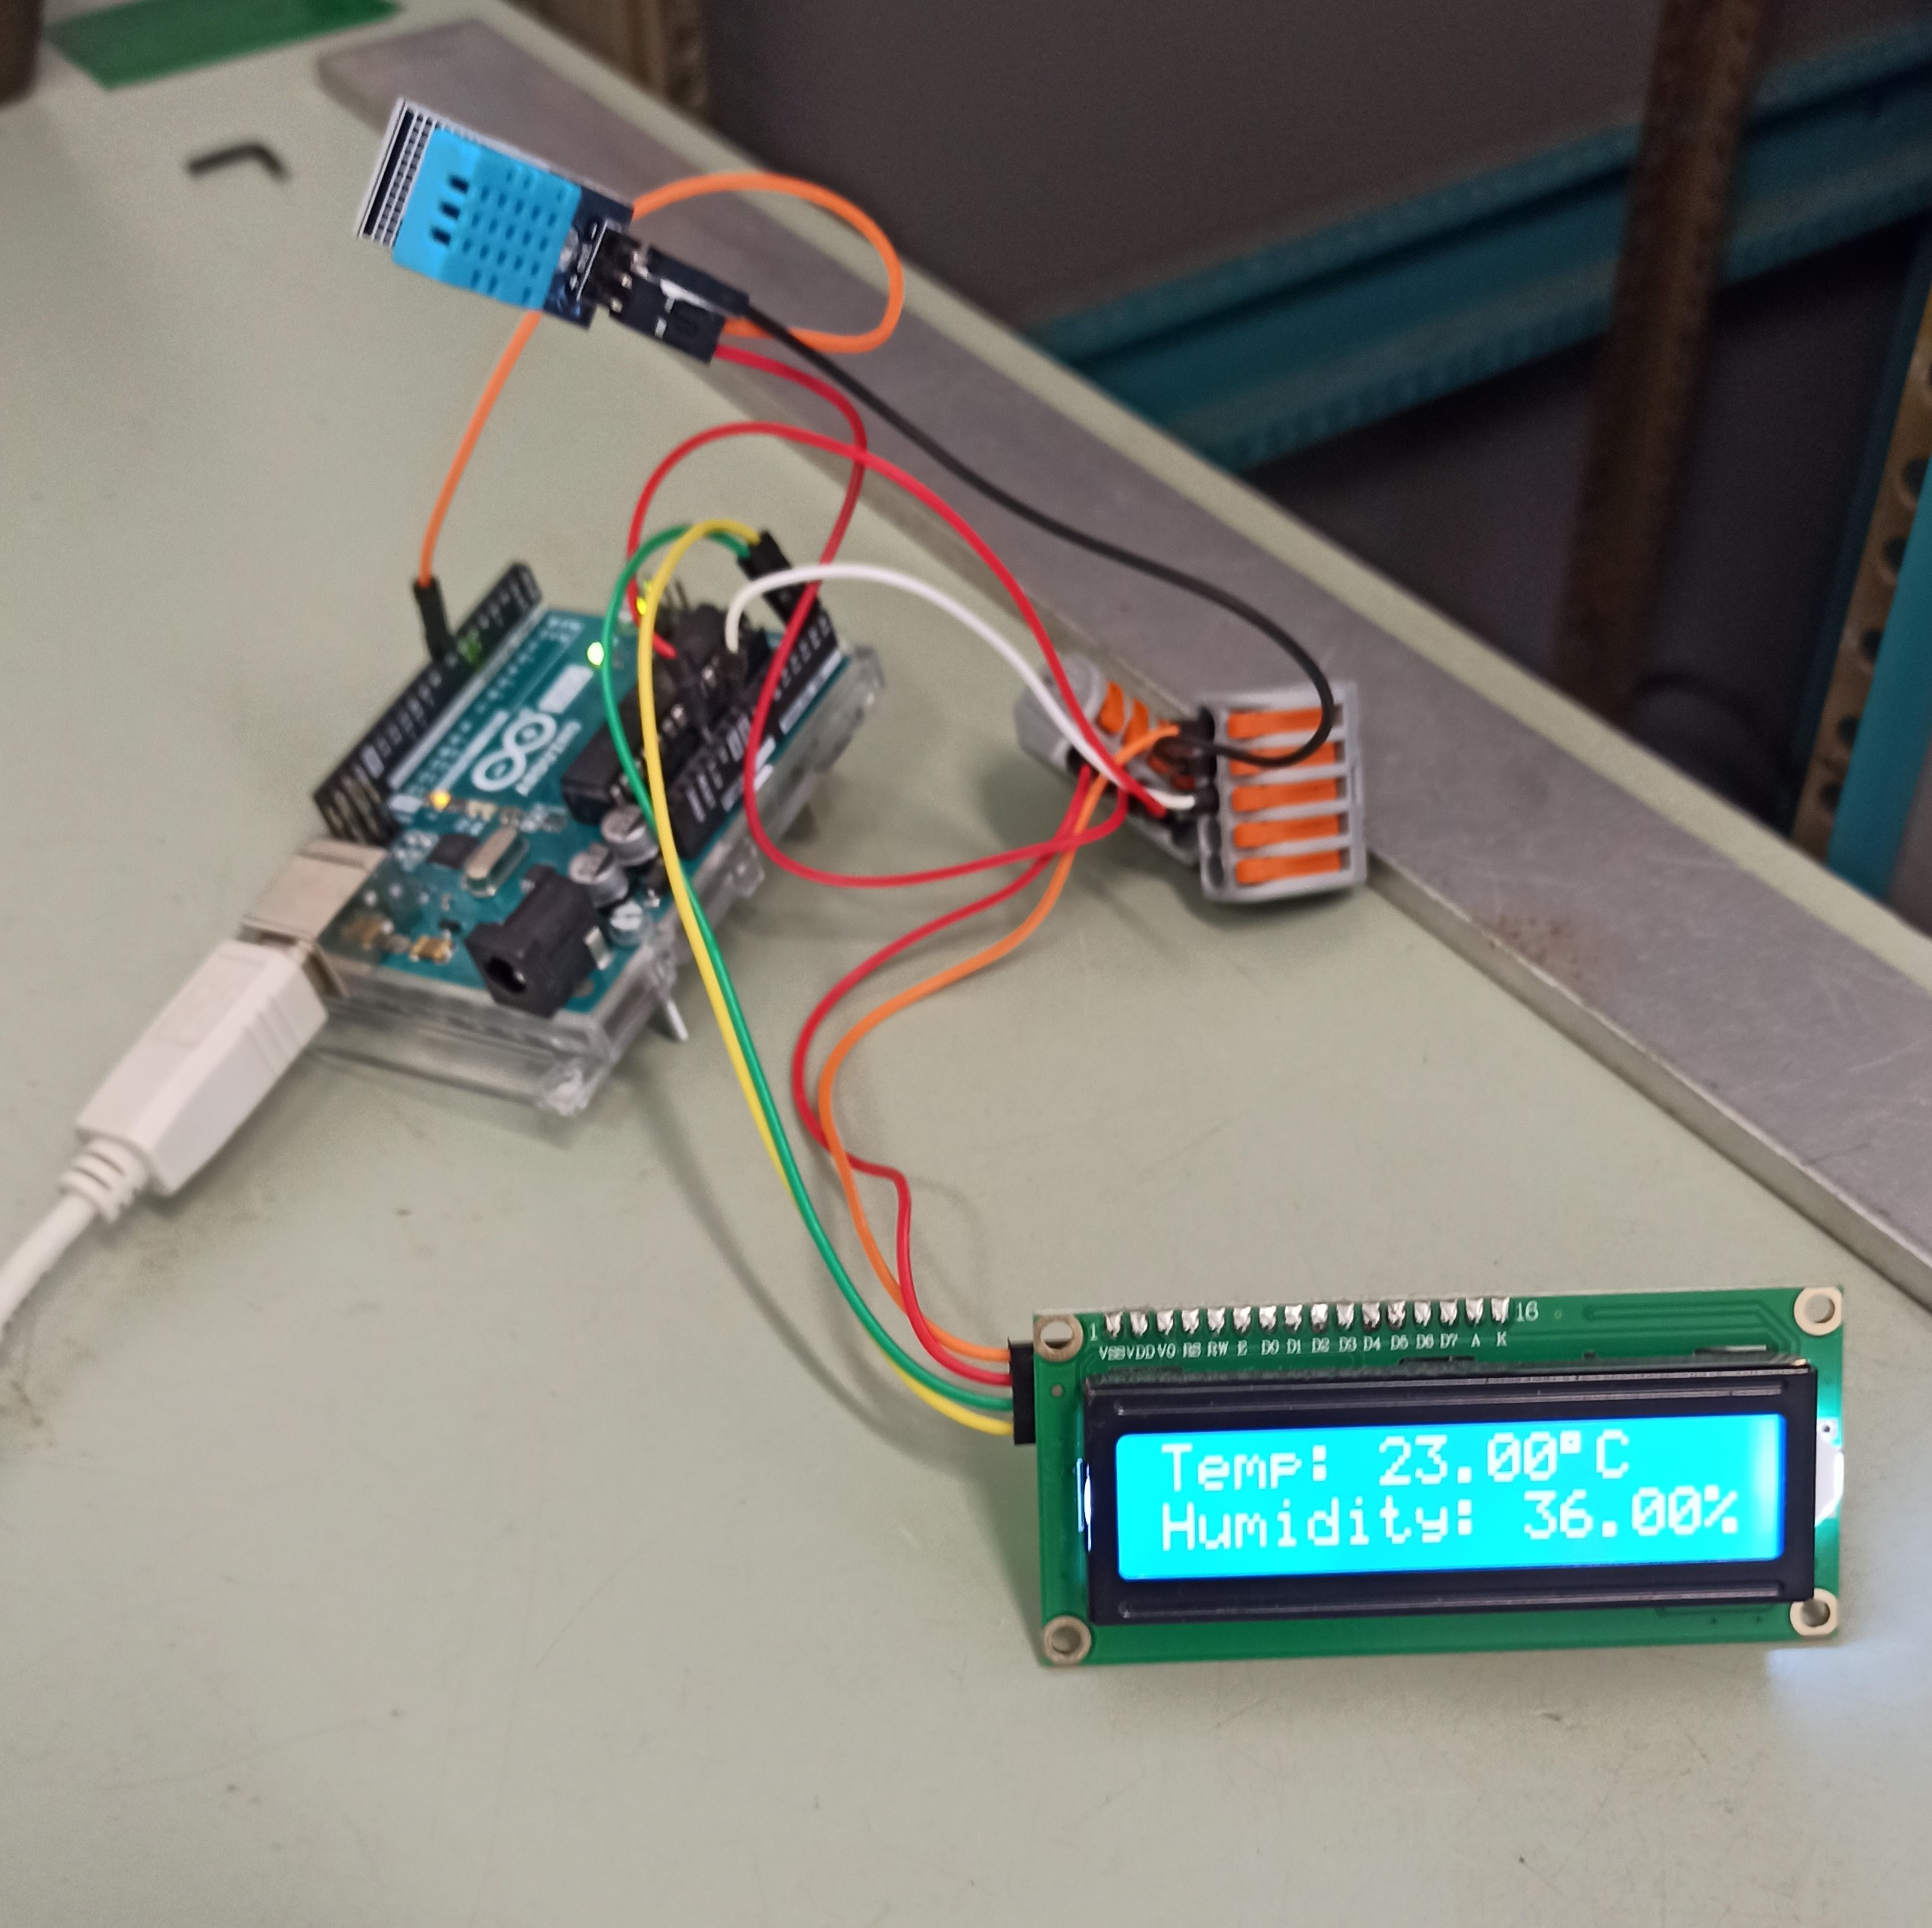
\includegraphics[scale=0.08]{Figures/Temperature_ relative_humidity}
	\decoRule
	\caption[Climatic conditions of the test]{Climatic conditions of the test in a closed room}
	\label{fig:Fig19}
\end{figure}

%----------------------------------------------------------------------------------------
%	SUBSECTION 3
%----------------------------------------------------------------------------------------
\subsection{MMCG specimen last preparation and Moisture Content reach}
To test the specimens at the weighted MC, plots as the \ref{fig:Fig15_a} were used. Indeed, by looking to their weight when they were out of the water, a MC was obtained, and by looking to the difference between the current MC and the weighted one can be given in terms of hours. So it was possible to have an approximation of the time before doing the experiments.

All the specimens were painted to obtain a pattern which allows a treatment of the images as explained before. Indeeed it will be necessary for MatchID to have speckles composed of a given number of pixels. A white first layer was added and a black point cloud was a second painting layer. All the paint used, are mate ones, and not brilliant ones. The dimension of the painted areas are not precisely defined. It is not necessary to paint the heels, because they were not studied. But even some painted zone are not really interesting as the extremity of MMCG specimen shapes. 
\begin{figure}[th]
	\centering
	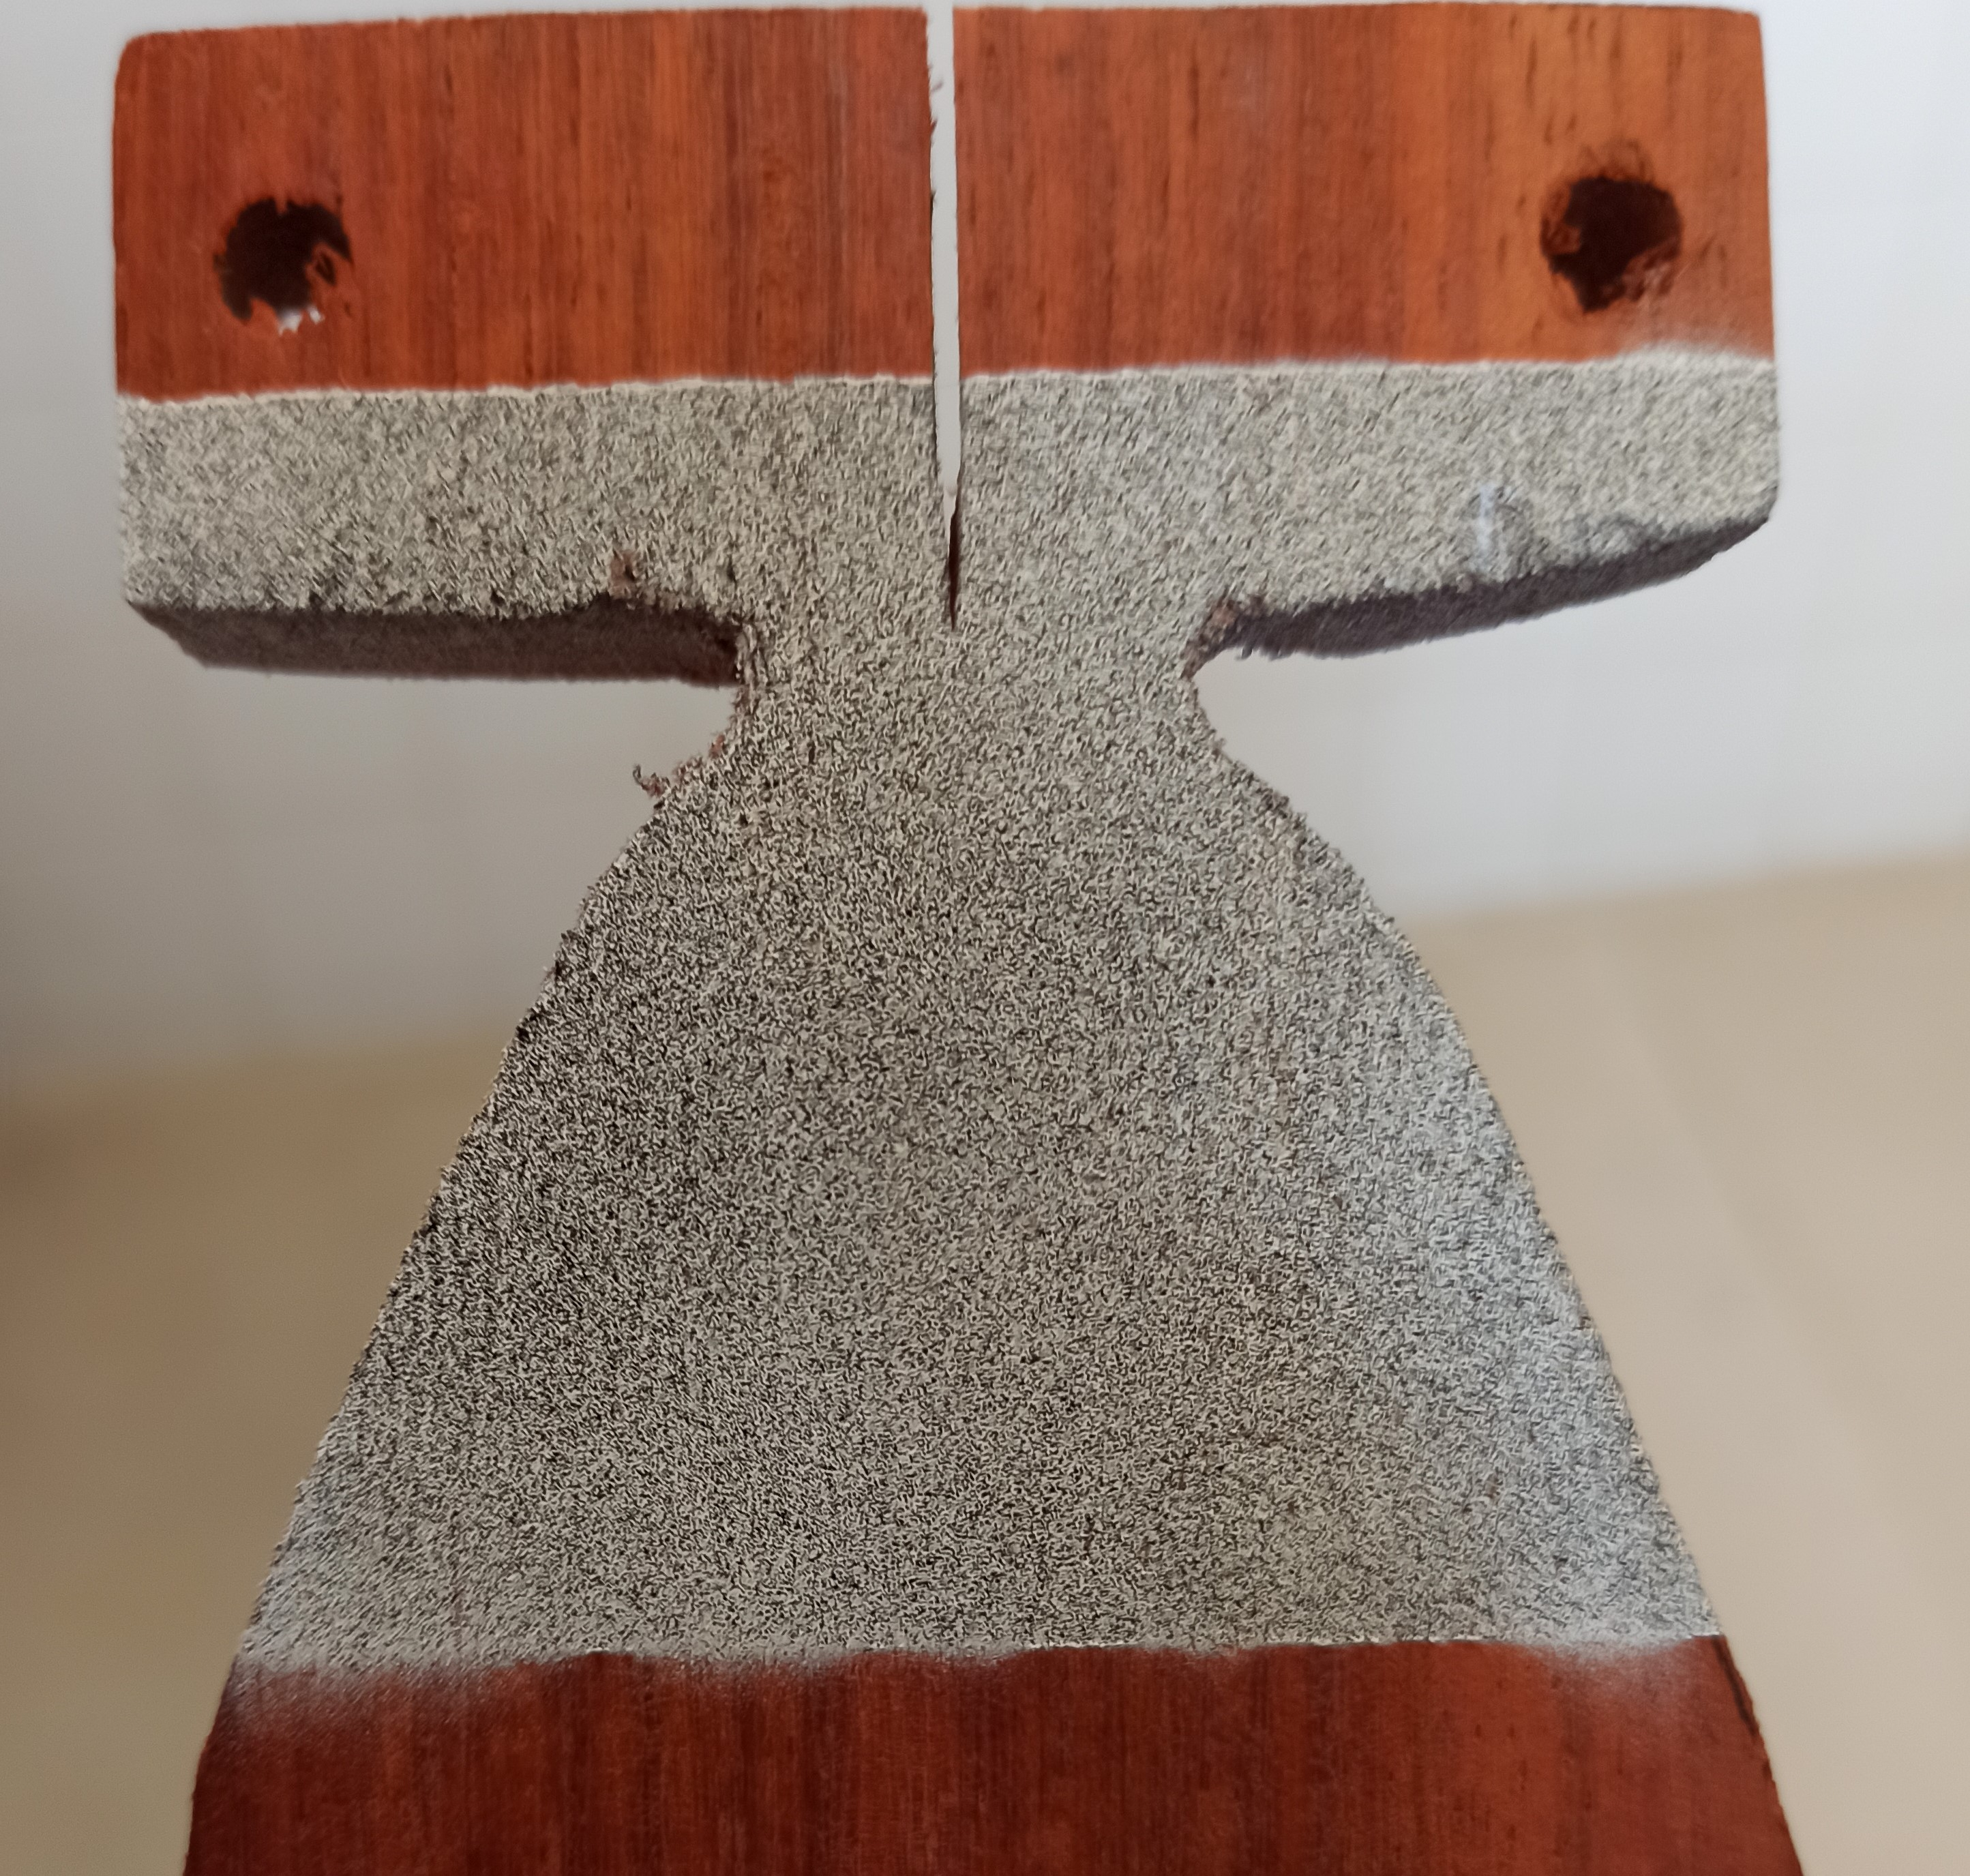
\includegraphics[scale=0.08]{Figures/Painted_specimen}
	\caption[Padouck painted specimen]{Padouck painted specimen before experimental test}
	\label{fig:paintedSpec}
\end{figure}
As it is presented on \ref{fig:paintedSpec} the characteristic pattern replace the grid from the grid method as used in \parencite{Reference7} or a markers tracking method like in \parencite{Reference18} work. The pattern is different for every specimen. From the second sample tested, a scale was added to the specimens. But finally this scale was not useful. Indeed, DIC images allow to fix some dimensions and measured others.
The precrack was measured again and more precisely with a caliper. The measure can change, due to the swelling of the wet specimens.

Dimensions as the crack length or the thickness of the specimens were measured again due to their evolution because of the swelling process. For some of the specimens, the grips were embedded in advance to remove some material which could distort the final weight. Then they are weighted a last time. The table \ref{tab:LastMC} presents the MC reached by all the specimens when there were tested.
\newpage
\begin{table}[th]
	\centering
	\begin{tabular}{cccc}
				
		\multicolumn{1}{c}{Name of   the specimen} & \multicolumn{1}{c}{dry Weight {[}g{]}} & \multicolumn{1}{c}{Tested weight} & \multicolumn{1}{c}{MC} \\ 
		\multicolumn{4}{c}{} \\ 
		\multicolumn{4}{c}{\cellcolor[HTML]{F4B084}room t° \& room MC} \\ 
		\multicolumn{1}{c}{E1O1} & \multicolumn{1}{c}{39,446} & \multicolumn{1}{c}{42,395} & \multicolumn{1}{c}{7,48\%} \\ 
		\multicolumn{1}{c}{E1O2} & \multicolumn{1}{c}{36,223} & \multicolumn{1}{c}{38,9057} & \multicolumn{1}{c}{7,41\%} \\ 
		\multicolumn{1}{c}{E1O3} & \multicolumn{1}{c}{35,496} & \multicolumn{1}{c}{38,108} & \multicolumn{1}{c}{7,36\%} \\ 
		\multicolumn{1}{c}{E1P1} & \multicolumn{1}{c}{52,243} & \multicolumn{1}{c}{54,867} & \multicolumn{1}{c}{5,02\%} \\ 
		\multicolumn{1}{c}{E1P2} & \multicolumn{1}{c}{61,411} & \multicolumn{1}{c}{64,652} & \multicolumn{1}{c}{5,28\%} \\ 
		\multicolumn{1}{c}{E1P3} & \multicolumn{1}{c}{61,493} & \multicolumn{1}{c}{64,507} & \multicolumn{1}{c}{4,90\%} \\ 
		\multicolumn{1}{c}{E1I1} & \multicolumn{1}{c}{51,67} & \multicolumn{1}{c}{54,858} & \multicolumn{1}{c}{6,17\%} \\ 
		\multicolumn{4}{c}{\cellcolor[HTML]{F4B084}room t° \& MC$\sim$30\%} \\ 
		\multicolumn{1}{c}{E2O1} & \multicolumn{1}{c}{34,219} & \multicolumn{1}{c}{40,914} & \multicolumn{1}{c}{19,57\%} \\ 
		\multicolumn{1}{c}{E2O2} & \multicolumn{1}{c}{35,511} & \multicolumn{1}{c}{41,601} & \multicolumn{1}{c}{17,15\%} \\ 
		\multicolumn{1}{c}{E2O3} & \multicolumn{1}{c}{36,862} & \multicolumn{1}{c}{43,8} & \multicolumn{1}{c}{18,82\%} \\ 
		\multicolumn{1}{c}{E2P1} & \multicolumn{1}{c}{63,15} & \multicolumn{1}{c}{72,273} & \multicolumn{1}{c}{14,45\%} \\ 
		\multicolumn{1}{c}{E2P2} & \multicolumn{1}{c}{64,803} & \multicolumn{1}{c}{74,965} & \multicolumn{1}{c}{15,68\%} \\ 
		\multicolumn{1}{c}{E2P3} & \multicolumn{1}{c}{63,154} & \multicolumn{1}{c}{71,832} & \multicolumn{1}{c}{13,74\%} \\ 
		\multicolumn{4}{c}{\cellcolor[HTML]{F4B084}room t° \& MC$\sim$20\%} \\ 
		\multicolumn{1}{c}{E3O1} & \multicolumn{1}{c}{37,436} & \multicolumn{1}{c}{46,485} & \multicolumn{1}{c}{24,17\%} \\ 
		\multicolumn{1}{c}{E3O2} & \multicolumn{1}{c}{32,745} & \multicolumn{1}{c}{41,772} & \multicolumn{1}{c}{27,57\%} \\ 
		\multicolumn{1}{c}{E3O3} & \multicolumn{1}{c}{36,449} & \multicolumn{1}{c}{46,434} & \multicolumn{1}{c}{27,39\%} \\ 
		\multicolumn{1}{c}{E3P1} & \multicolumn{1}{c}{64,831} & \multicolumn{1}{c}{76,897} & \multicolumn{1}{c}{18,61\%} \\ 
		\multicolumn{1}{c}{E3P2} & \multicolumn{1}{c}{65,323} & \multicolumn{1}{c}{77,427} & \multicolumn{1}{c}{18,53\%} \\ 
		\multicolumn{1}{c}{E3P3} & \multicolumn{1}{c}{60,43} & \multicolumn{1}{c}{74,757} & \multicolumn{1}{c}{23,71\%} \\ 
		\multicolumn{4}{c}{\cellcolor[HTML]{F4B084}fridge samples} \\ 
		\multicolumn{1}{c}{E4O1} & \multicolumn{1}{c}{40,233} & \multicolumn{1}{c}{52,592} & \multicolumn{1}{c}{30,72\%} \\ 
		\multicolumn{1}{c}{E4P1} & \multicolumn{1}{c}{57,116} & \multicolumn{1}{c}{64,696} & \multicolumn{1}{c}{13,27\%} \\ 
		\multicolumn{1}{c}{E4I1} & \multicolumn{1}{c}{46,467} & \multicolumn{1}{c}{67,599} & \multicolumn{1}{c}{45,48\%} \\ 
		\multicolumn{4}{c}{\cellcolor[HTML]{F4B084}oven sample} \\ 
		\multicolumn{1}{c}{E5O1} & \multicolumn{1}{c}{38,104} & \multicolumn{1}{c}{40,172} & \multicolumn{1}{c}{5,43\%} \\ 
		\multicolumn{1}{c}{E5P1} & \multicolumn{1}{c}{59,767} & \multicolumn{1}{c}{66,339} & \multicolumn{1}{c}{11,00\%} \\ 
		\multicolumn{1}{c}{E5I1} & \multicolumn{1}{c}{51,828} & \multicolumn{1}{c}{66,718} & \multicolumn{1}{c}{28,73\%} \\ 
		\multicolumn{4}{c}{\cellcolor[HTML]{F4B084}resting samples} \\ 
		\multicolumn{1}{c}{Pbis} & \multicolumn{1}{c}{64,574} & \multicolumn{1}{c}{67,301} & \multicolumn{1}{c}{4,22\%} \\ 
		\multicolumn{1}{c}{Pter} & \multicolumn{1}{c}{60,379} & \multicolumn{1}{c}{63,418} & \multicolumn{1}{c}{5,03\%} \\ \hline
	\end{tabular}
	\caption{Moisture Content in every tested samples}
	\label{tab:LastMC}
\end{table}
\newpage
%----------------------------------------------------------------------------------------
%	SUBSECTION 4
%----------------------------------------------------------------------------------------
\subsection{Difficulties and issues}

One of the main problem results of MMCG shapes and the small distance between holes and specimen extremities. It involves several cracks in the heel between the hole and the extremity of the sample. It prevents the observation and analysis of the fracture. This solution which was induced by previous work as \parencite{Reference7} is the use of washers. Indeed, by applying a compressive tension on each side of the specimen, it reduces the stress applied on the holes and it distributes the load in a wider area (the washers surface). \parencite{Reference7} have glued this washer in previous work. In this one it was chosen to strength screw the nut to increase the compressive load created by the washers. Without torque wrench, it is difficult to give an average of the washers constraint exerted. But then this tool was find and used. An approximation of the couple needed to screw and avoid the crack in the hole area is 6.9\si{\newton\per\meter}. By using the \ref{eq:Washers compressive load} formula below, an average is given. Indeed, the medium diameter and the characteristic diameter are given by mechanics table as the real screw thread. The friction factor between wood and steel is consider at 0.3, even if it could be increased for an Okoume specimen and decreased on a Padouck one. Then, the load applied on the wood by the washers is determined.
\begin{equation}
	\begin{array}{c}
	T_{a}=F\cdot\dfrac{d_{m}\cdot (\pi\mu d_{m} + l)}{2(\pi d_{m}-\mu l)} + F\cdot\mu\cdot\frac{d_{c}}{2}
	\\
	\\
	\left\{
	\begin{array}{llllll}
		T_{a}: & $Torque load$ & 6.9 &\si{\newton\meter} \\
		F: & $Compressive load$ & . & \si{\newton} \\
		d_{m}: & $medium flank diameter$ & 3.545 & \si{\milli\meter} \\ 
		\mu: & $friction factor $ & 0.3 & . \\
		d_{c}: & $characteristic diameter of the friction crown$ & 5.6 & \si{\milli\meter} \\
		l: & $real screw thread$ & 0.7 & \si{\milli\meter} \\
	\end{array}
	\right.
	\end{array}{l}
%	\\
%	\\
%	$Which become :$
%	\\
%	\\
%	F=6.9\cdot\dfrac{d_{m}\cdot (\pi\mu d_{m} + l)}{2(\pi d_{m}-\mu l)} + F\cdot\mu\cdot\frac{d_{c}}{2}
	\label{eq:Washers compressive load}
\end{equation} 
The result gives an approximation of 5.4\si{\newton} which is the load allowing to provide fracture in the hole area.

Another problem is linked to the first one. No data were available for Iroko specie. Indeed, the three specimens have broken near the hole, even with washers uses. This specie seems more fragile than the others ones. Moreover it is a stringy wood. Some parts of the specimen can be removed just by friction, which is not the case for the others species. So the experiments on Iroko were not concluant.

As presented before, another problem is the determination of a precise moisture content inside the specimens. Due to the fast decrease of MC, even with a first scheme of the behavior, it was impossible to predict the MC in advance. Indeed, the relative humidity and the temperature evolve too much during the days before a test. 

Finally a difficulty can appear in the case of an experiment done alone. Indeed, it takes many time to setup all the presented equipments. All the experiments were done with three personnes working on it. Even at three, almost 10 minutes were taken for each test setup and 3 others for the test itself. It means that, if many specimens should be tested, they will lose MC during the experiments of the previous samples. Moreover, some coordination is needed to proceed to the test, it is easier to put the grips through the specimens with somebody rising the press to demand, two persons to launch the record and the beginning of the test in the same time.

%----------------------------------------------------------------------------------------
%	SECTION 2
%----------------------------------------------------------------------------------------
\section{Results}

%----------------------------------------------------------------------------------------
%	SUBSECTION 1
%----------------------------------------------------------------------------------------
\subsection{Settings to obtain data}

%MatchID setting to process and Python modification
Even if the Python code was done and well prepared before the post processing task, many details needed to be modified.

Indeed, first the loads had not the expected shapes. Due to the preload applied to fix the specimens, all the curves did not begin at 0\si{\newton}. So a shift was necessary to consider the lower value as the 0 one. By doing this, it appears that the displacement did not begin at 0 anymore. Then a second shift was done to extrapolate the curve shape and create a virtual point beginning at [0,0]. This shift is visible on the \ref{fig:Pdel_shift}
\begin{figure}[th]
	\centering
	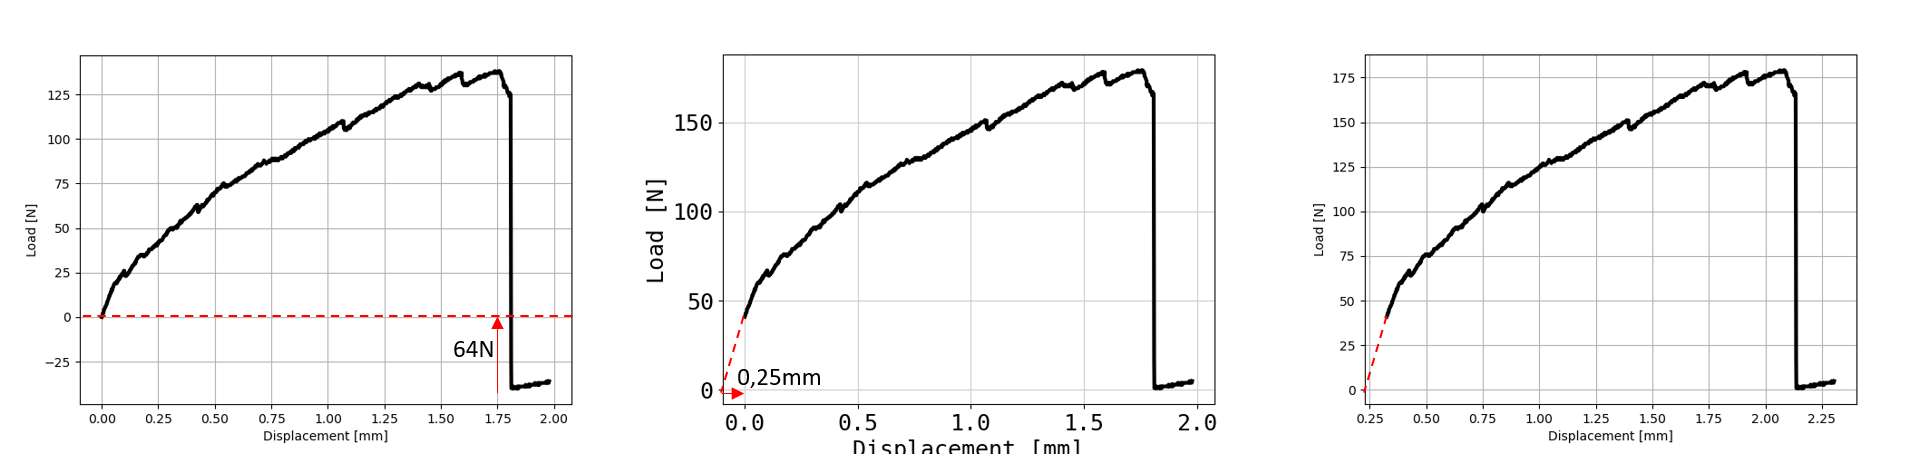
\includegraphics[width=\textwidth]{Figures/Pdel_shift}
	\caption[P-$\delta$ curve shifting processus]{P-$\delta$ curve shifting processus for the first Okoume specimen of the first experiment}
	\label{fig:Pdel_shift}
\end{figure}

\begin{customFrame}
minL=np.min(Load)-1
Load = Load-minL
\end{customFrame}
By substracting the lower value of the load on all the load values, as it is done overhead, it avoids the negatives values. Indeed, it does not have sens, because no compressive loads were applied on the specimen.
Then, looking to the first part of all the P-$\delta$ curves, it is visible that the first part is a linear one. The load increases and the displacement do the same. There is no crack propagation in this part, so the load will not decrease allowing a linear behavior. So by using remotes points on this linear part, as the first one and the 300th, and divide the subtract of both by the number of elements between them, a step is obtained. This step, as shown below, is used in a while loop.   
\begin{customFrame}
X1 = Displ[0]
X2 = Displ[300]
Y1 = Load[0]
Y2 = Load[300]
pas = (Y2-Y1)/300
pas_bis = (X2-X1)/300
i = Y1
j = X1
k = 0

while i > 0:
	i = i-pas
	j = j+pas_bis
	k=k+1
	print('k vaut : %d' %k)

shift_right = j

Displ = Displ+shift_right	
\end{customFrame}
This while loop, subtract the step until the abscissa axis is crossed. Looking to the difference between the first abscissa value and the new one obtained after the cycles, the displacement shift is determined. These modifications allow to use real values of the load as presented on \ref{fig:Pdel_shift}. The main problem of this method, it that the tests are not always completely destroyed. This fact does not allow to have a real first value. Indeed, in these cases, the preload will be considered as the first value, while the collapse of the specimen gives a more precise idea of the load without resistance from the material. As presented in \ref{fig:Pdel_shift}, which is a great example, the end of the test shows the real 0 value, around -48\si{\newton} and permit to have the preload, around this value. But looking at the different P-$\delta$ curves, no pattern can be identified. So it is impossible to put a constant preload on every specimens. It could involve mistakes.
 
Then the "CODpair" must be chosen by the user. It means that looking to all the shapes that the CTOD evolution can have, it is necessary to choose the most accurate one. Indeed, it must be remind, that the chosen pair of subsets as shown on \ref{fig:subest_chosen} have to be the closest to the crack tip to give displacement accuracy, but far enough to avoid a loose of information (if they are placed into the crack). After this study, databases are updates with the CODpair chosen. As presented on \ref{fig:CODpairchos} a plot was created, showing the $w_{I}$ shapes used, thanks to the chosen COD pair in blue. The plot also compared this curve with the one done with the COD pair lower and the upper, in order to prove for every specimen, that the COD pair chosen, can not be more precise, and was similar to the upper one. 

\begin{figure}[th]
	\centering
	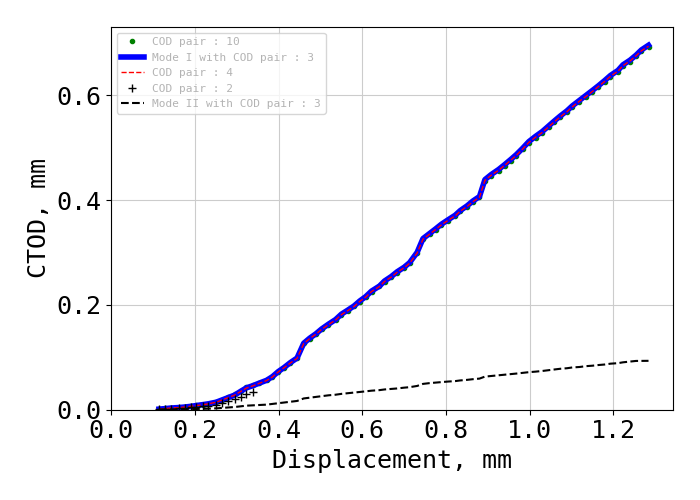
\includegraphics[scale=0.4]{Figures/CODpairchos}
	\caption[Crack tip opening displacement depending on COD pair input]{Crack tip opening displacement depending on hydraulic press displacement compared according to COD pair input into database}
	\label{fig:CODpairchos}
\end{figure}

At least, alpha parameter have to be chosen. Indeed, it is a determinant parameter in order to have the crack length values. As explained and shown on \ref{fig:Fig11}, it must be as the CODpair, precise but not wrong, here due to the noise. By compiling the a(t) evolution depending on the images recorded for several alpha values, as in \ref{fig:a_alpha}, it is possible to have an idea on the alpha value needed to have the greatest a(t). This choice is determinant in order to have a precise  a(t). Indeed, the alpha parameter must be as little as possible to have the entire crack length evolution. So regarding each specimen crack length, it is possible to eliminate several candidates. On this example \ref{fig:a_alpha}, it is possible to avoid the use of the purple curve, relative to the alpha value equal to 7. This alpha value does not allow the study of the entire crack length which can reach, on this example, almost 50\si{\milli\meter}. Then in the case of specimens as \ref{fig:a_alpha}, the choice is hard. 
\begin{figure}[th]
	\centering
	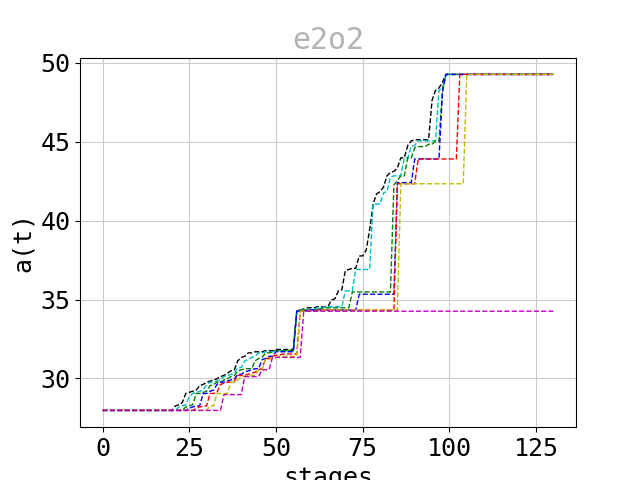
\includegraphics[scale=0.4]{Figures/a_alpha}
	\caption[crack length evolution depending on alpha]{crack length evolution depending on alpha for the second Okoume specimen of the second experiment}
	\label{fig:a_alpha}
\end{figure}
A solution to find the best alpha value and the best crack length to compute G, is looking to the next plot :
\begin{customFrame}
j = 30
fig = plt.figure()
plt.imshow(UY[:, :, j])
plt.plot(UY.shape[1]-crackL_J_pixel_X[j, chos_alp],crackL_J_pixel_Y[j, chos_alp],'sr')
plt.colorbar()
plt.title(Job)
plt.show()
\end{customFrame}
By the variation of the j parameter, which represents the stages, so images of the ZOI, and looking to the red dot create to follow the crack tip, it is possible to precise the choice. The red dot must be as close as possible to the crack tip. A lot of time, even at a 0 alpha parameter, which is equal to 1 (in Python the 0 is considered as the first value), the red dot is far from the crack tip. It means that the determination of the alpha will not involve mistakes. So the chosen one is the smaller alpha. But regarding his curve shape, and in order to avoid the noise, the smallest value is not always the chosen one. The black curve from \ref{fig:a_alpha} represents the alpha equal to 0. The shapes of the curves look to smooth and it is preferred to use curves which are more geometrically simple. In this example, alpha value as the 2 one (in green) or the 3 one (in dark blue) could be chosen. Indeed, they are made of steps, and reach the same a(t). The smallest is chosen, so in the database, the e2o2 specimen is computed with alpha equal to 3.

Then the G is compared. Two methods are submitted. The first one is the one presented in the previous chapter with \ref{eq:Energy release rate equation}. But another one use the compliance derivate by the crack length. Indeed, the C is defined as in \ref{eq:Compliance depending on the crack length}

\begin{equation}
	\begin{array}{l}
		C= m\cdot a^{3} + n
		\\
		\\
		\left\{
		\begin{array}{llll}
			C: & $Compliance$ \\
			m: & $slope$ \\
			a: & $crack length$ \\ 
			n: & $moisture content$ \\
		\end{array}{}
		\right.
	\end{array}{}
	\label{eq:Compliance depending on the crack length}
\end{equation}   

Here C is linked to a(t) parameter and then, by derivating it, it involves an equation of G presented as in \ref{eq:G_method2}. This method can be a better one, because it takes more in account the influence of the crack length on the studied specimen. 

\begin{equation}
	G_{I}= \frac{P^{2}}{2B}\cdot3ma^{2}
	\label{eq:G_method2}
\end{equation}   
%----------------------------------------------------------------------------------------
%	SUBSECTION 2
%----------------------------------------------------------------------------------------
\subsection{Results at room temperature and room humidity}

First, the P-$\delta$ curves were plotted. The specimens were compared regarding to their MC before being tested. The row data gives results as the \ref{Pdel_room_MC} ones. A pattern was searched to find a solution to the preload put on every specimen. But without real scheme allowing to improve the curves, the shifting process explained before was used.
\begin{figure}[h]
	\centering
	\begin{subfigure}{0.48\linewidth}
		\centering
		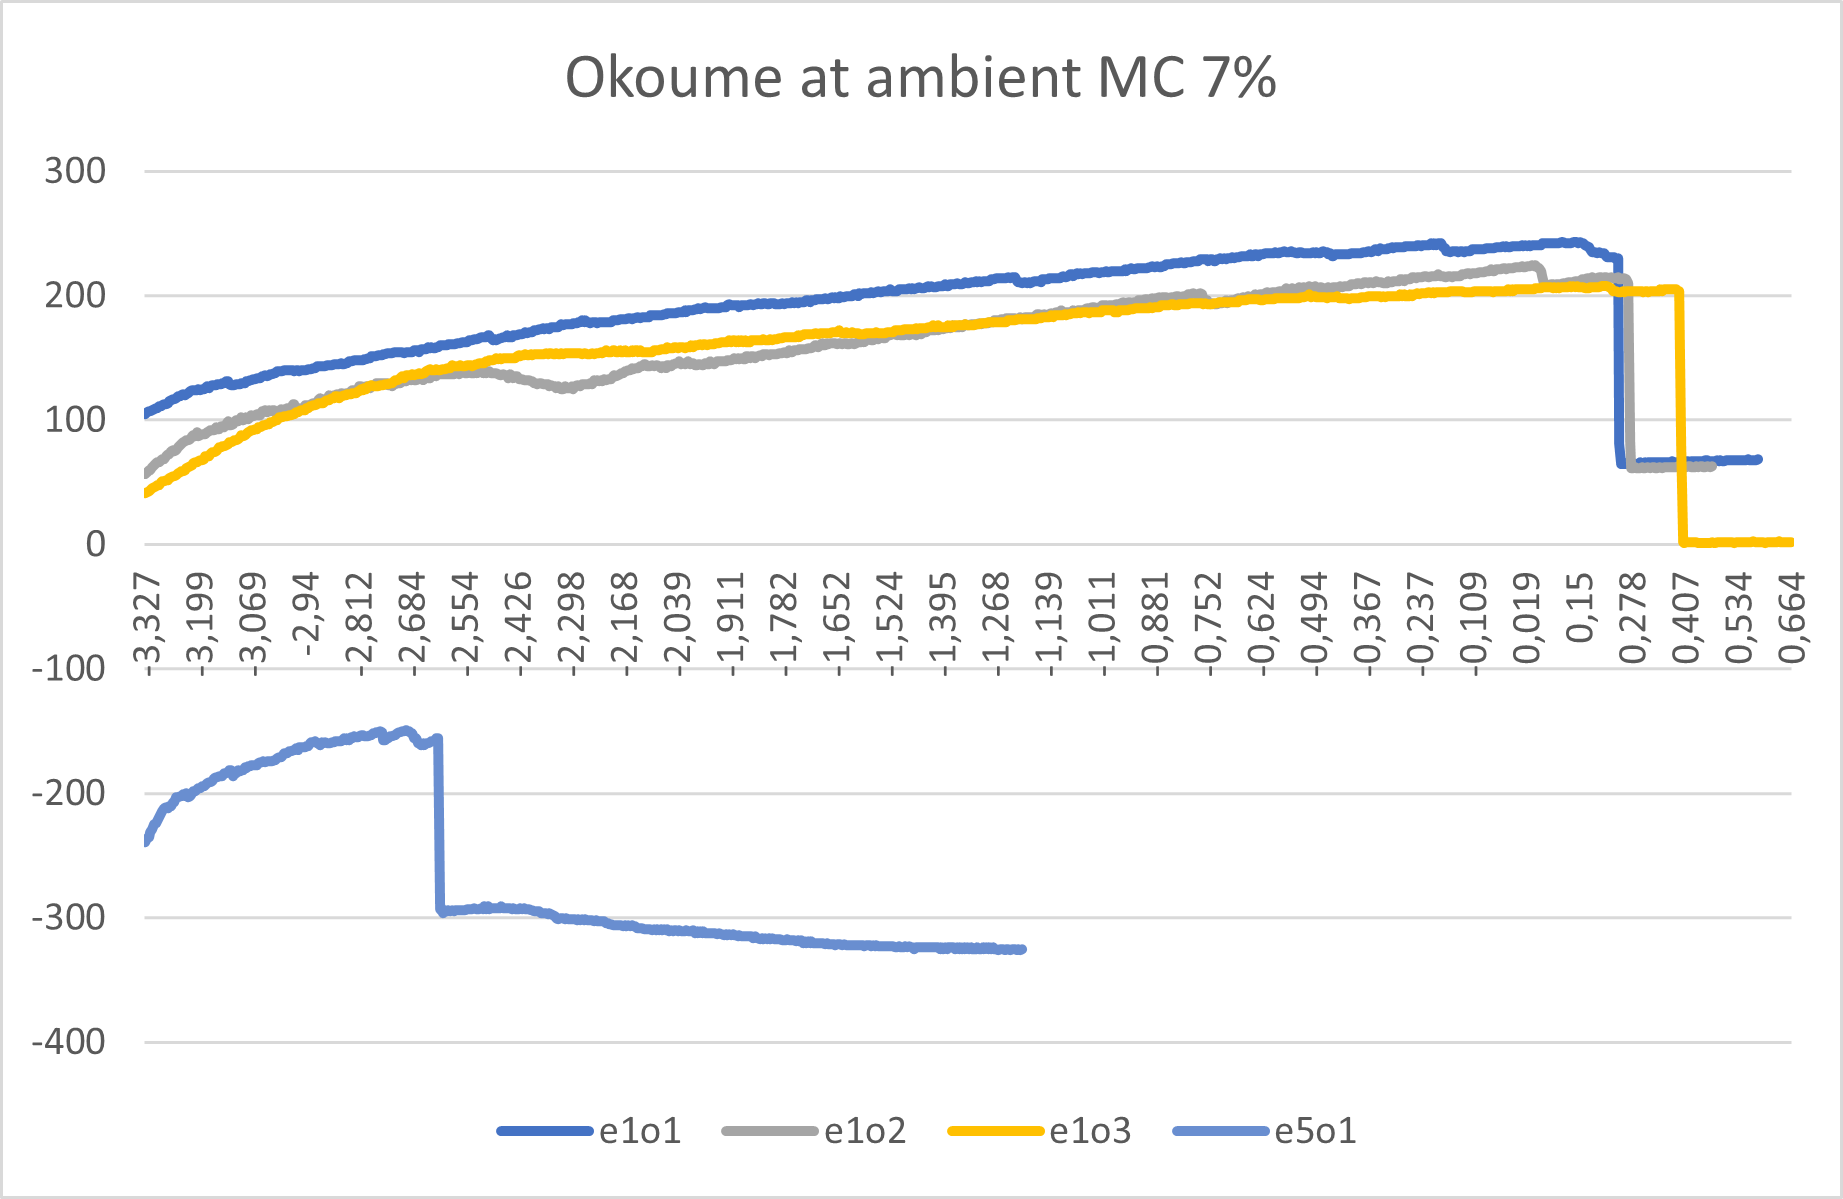
\includegraphics[scale=0.5]{Figures/PDelt_OKambient}
		\decoRule
		\caption[Okoume specimens tested at ambient moisture content]{P-$\delta$ curves of Okoume specimens tested at ambient moisture content approximately 7\%}
		\label{fig:Ambient_MC_Ok}
	\end{subfigure}
	\hfill
	\begin{subfigure}{0.48\linewidth}
		\includegraphics[scale=0.5]{Figures/PDelt_padambient}
		\decoRule
		\caption[Padouk specimens tested at ambient moisture content]{P-$\delta$ curves of Padouk specimens tested at ambient moisture content approximately 5\%}
		\label{fig:Ambient_MC_Pad}
	\end{subfigure}
	\caption{P-$\delta$ curves at normal MC}
	\label{Pdel_room_MC}
\end{figure}

The padouck specimens, which have been broken by a fracture near the fixation hole, was Pbis. It is one of the specimen, which must had been tested at this MC. 
Raw data are also composed of the important quantity of images recorded by the camera. Indeed, it appears that many experiments took between 2 and 3 minutes, using a 1Hz frequency of recording, it gives more than 120 images to treat.
By running the modified Python program, other results were found.

The Crack length first :

\begin{figure}[th]
	\centering
	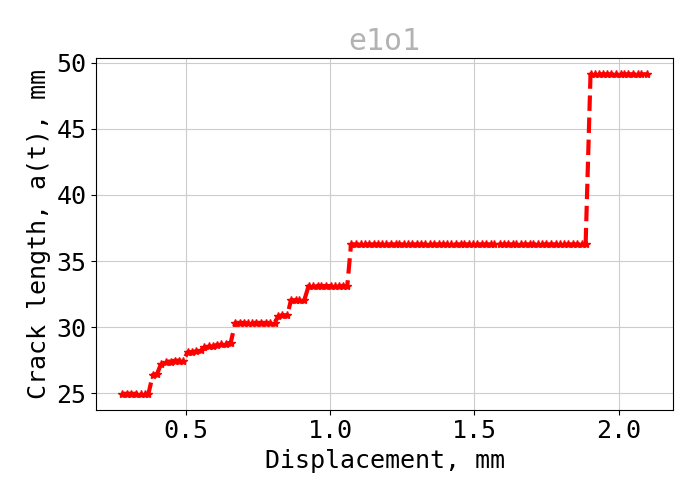
\includegraphics[scale=0.4]{Figures/e1o1_a}
	\caption[crack length evolution depending on hydraulic press displacement]{crack length evolution depending on servohydraulic test machine displacement.}
	\label{fig:e1o1_a}
\end{figure}

As presented, there are, as expected, different steps reach. It is due to the crack propagation which is developed gradually. Indeed, on some images, bridges do not allow the fracture to append linearly. When these bridges break, the crack propagates involving a new step. It is interesting to have a look at all the plots of this crack length propagation presented in \ref{E1o_a} and \ref{E1p_a}. Padouck specimens crack were impressive because they occurs faster. It was more visible during the real experiment, but an observation on the plots, allows to understand that the crack propagation for Padouck specimens were longer and occurs suddenly. This fact make sens, looking to previous work on the subject, Padouck has a more brittle rupture than Okoume. Okoume specimens were not entirely collapsed during the tests. More bridges were visible and it looks like an elastic material. This curves shapes permit to forecast energy release rate values appearances.

Indeed, the next parameter computed was the G one :

The data from Python were directly plotted, and all these curves are also presented in \ref{E1o_G} and \ref{E1p_G}. But the values used to create these figures were also imported, in order to allow a comparison of the Energy release rate and the MC. A last plot was made of all the specimens submitted at room climatic conditions (20\textcelsius and at a relative humidity around 45\%).
\begin{figure}[th]
	\centering
	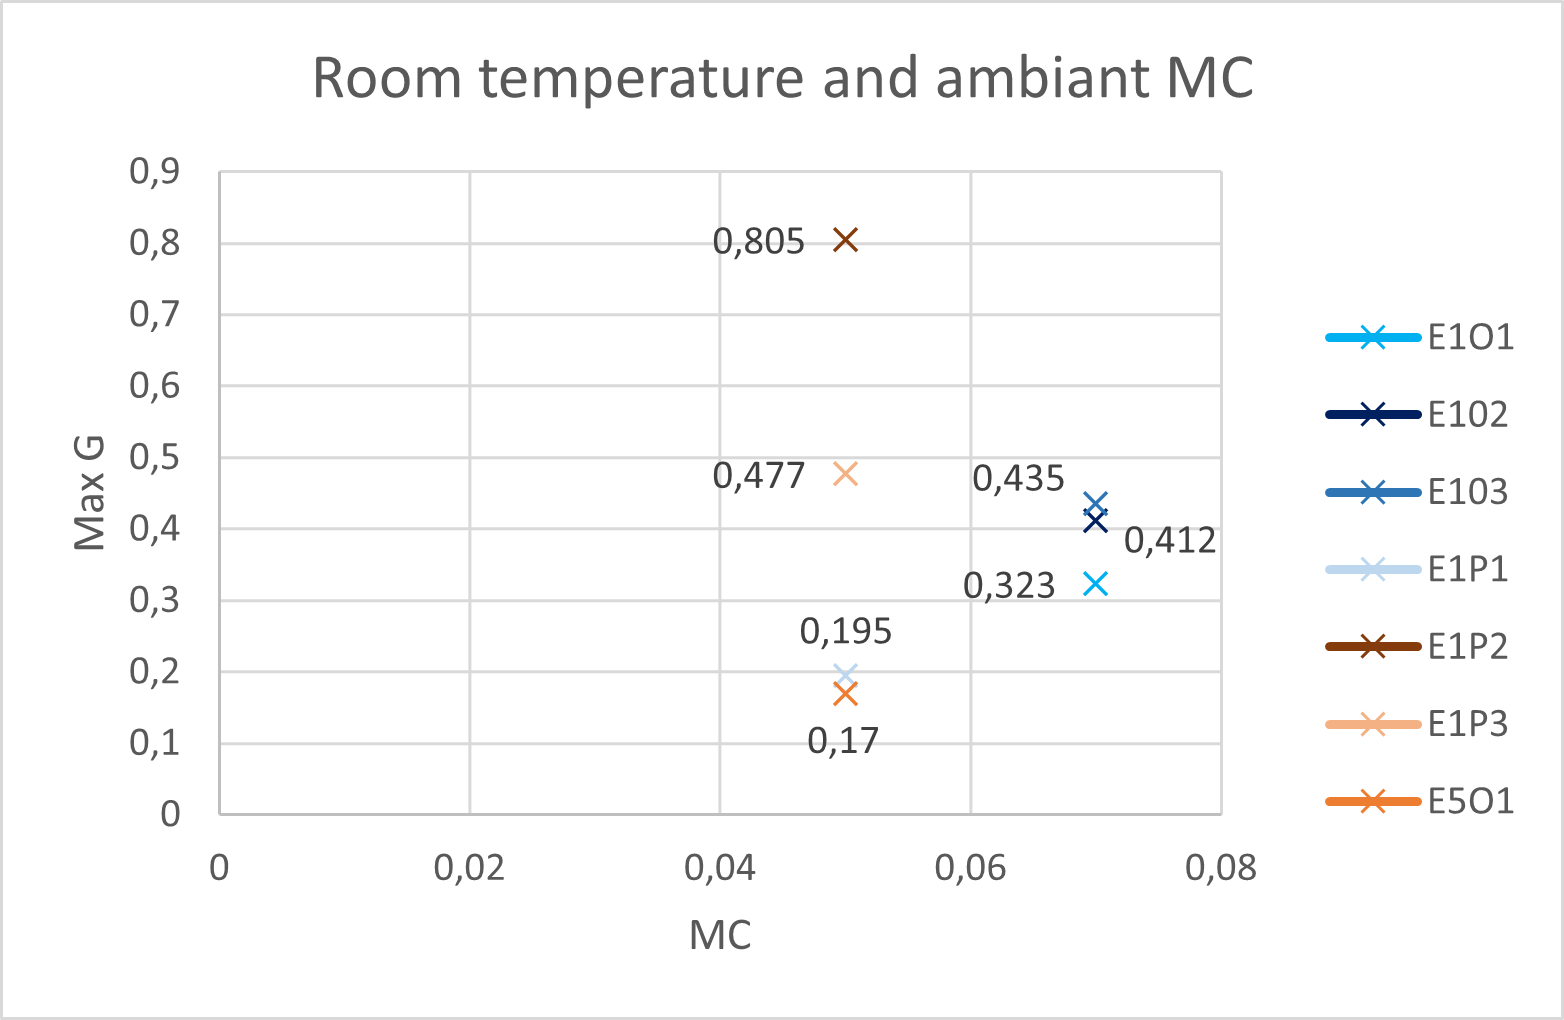
\includegraphics[width=\textwidth]{Figures/Res_MCamb}
	\caption[G depending on MC in room conditions]{Energy release rate from tested specimens depending on MC in room conditions}
	\label{fig:Res_MCamb}
\end{figure}

This plot \ref{fig:Res_MCamb} allows to have a view of the big picture. The points only illustrate the G maximal value from each plot. So it is an addition to the \ref{E1o_G} and \ref{E1p_G} plots. It also presents some surprising results which will be discussed in the next chapters.

And finally, $\sigma$ parameter is analyzed, in order to obtain a final curve, representing the cohesive law. It is defined by \ref{eq:sigma}. This parameter takes care of the CTOD computed by Python, which can be a wrong value if the alpha parameter was not well chosen. This factor can explain strange shapes

\begin{equation}
\sigma = \frac{G}{w_{I}}
\label{eq:sigma}
\end{equation} 

Then the cohesive law is the plot of $\sigma$ depending on $w_{I}$. Again, all the cohesive laws from this experiment are presented in \ref{E1o_colaw} and \ref{E1p_colaw}. The literature show cohesive laws with shapes as \ref{fig:E1P1_colaw} or \ref{fig:E1P2_colaw} ones. So before analyzing the data, by having a critical view on the plots, it is possible to discuss the values veracity.

\newpage
%----------------------------------------------------------------------------------------
%	SUBSECTION 2
%----------------------------------------------------------------------------------------
\subsection{Results with specimen at a moisture content around 20\% }

As explain before, the curves shown on \ref{fig:Pdel_20_MC} were made before the shifting process from Python. This is the reason of the negative values. It appears that the load necessary to the collapse of Okoume specimens are around 270\si{\newton} while these values for Padouck specimens are really different from one to another. As it is presented in \ref{tab:LastMC}, the MC reach is not homogeneous and could explain the steps between the results. 
\begin{figure}[h]
	\centering
	\begin{subfigure}{0.48\linewidth}
		\centering
		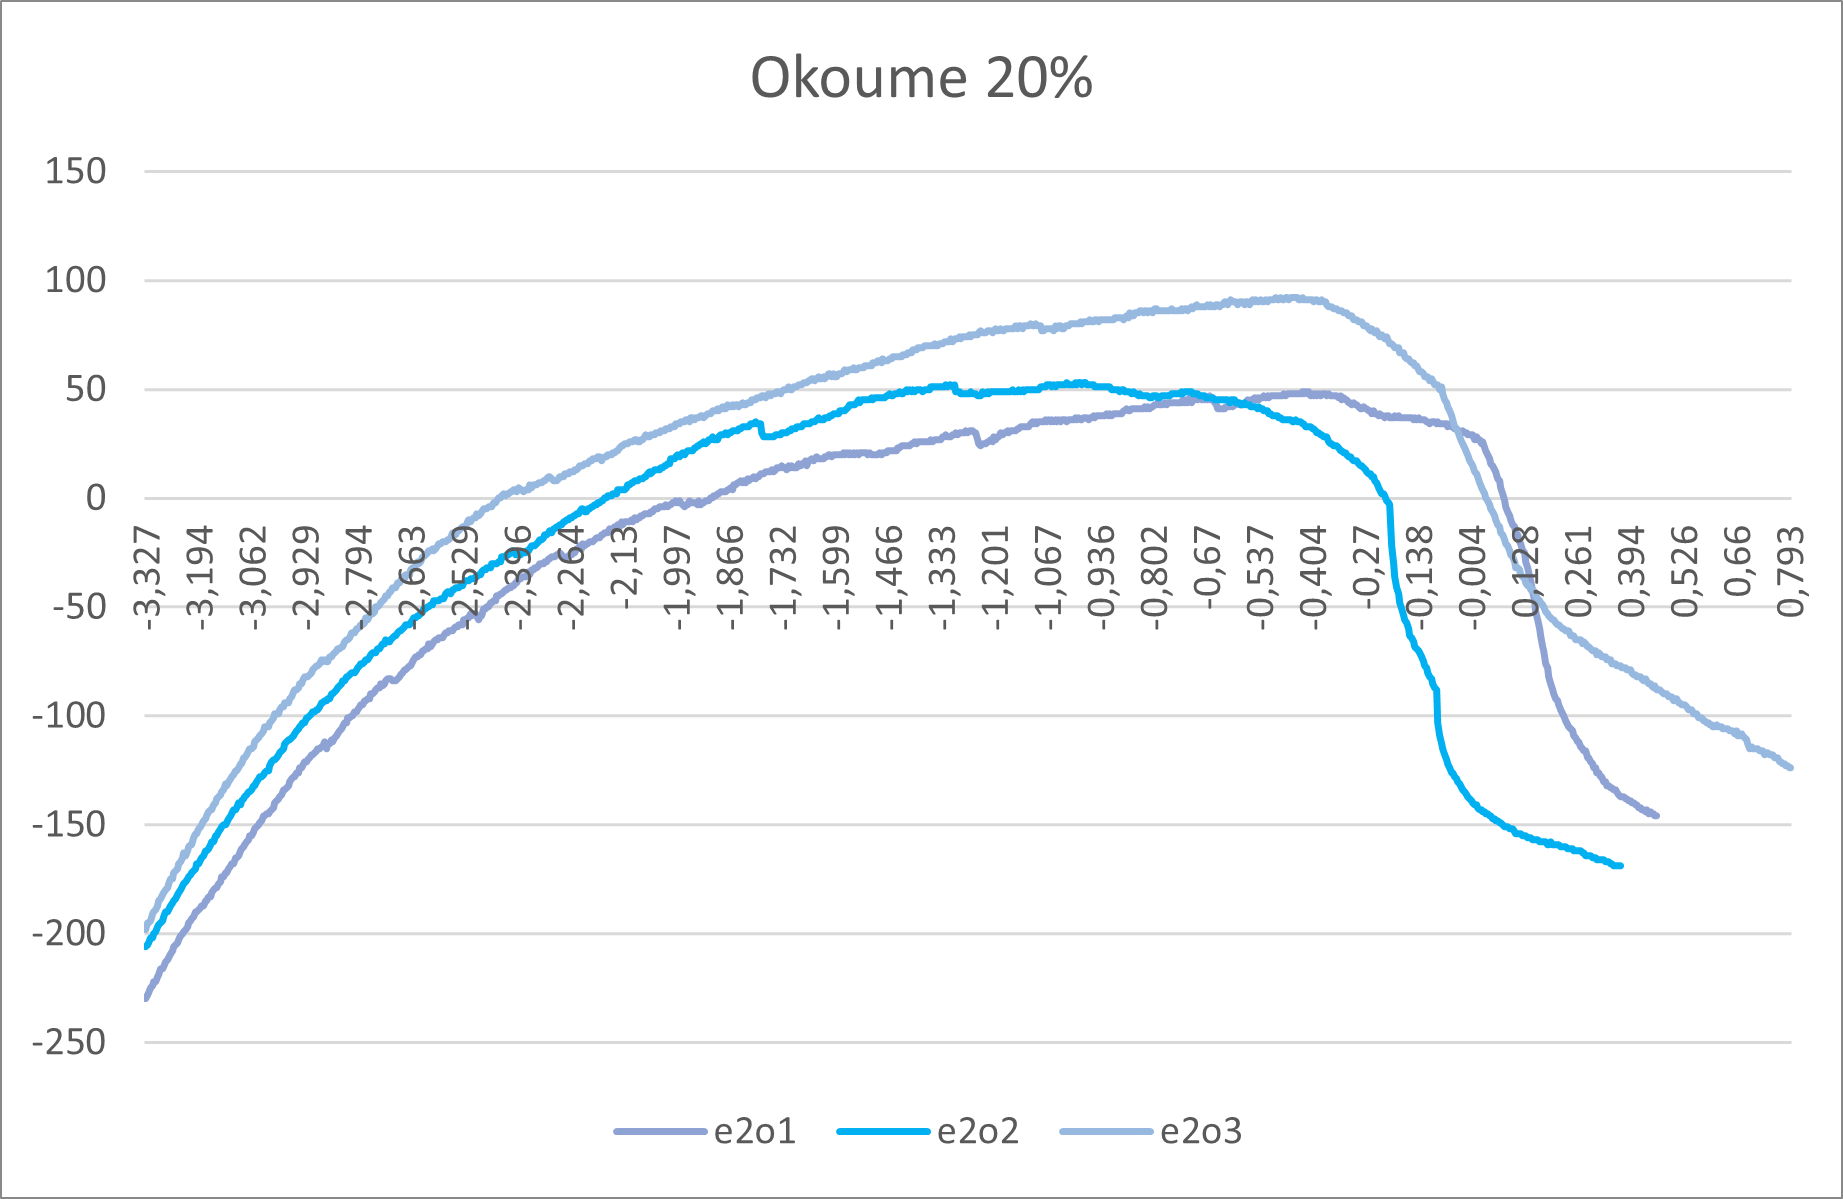
\includegraphics[width=\textwidth]{Figures/PDelt_OK20}
		\decoRule
		\caption[Okoume specimens tested at 20\% moisture content]{P-$\delta$ curves of Okoume specimens tested at a moisture content around 20\%}
		\label{fig:MC_Ok_20}
	\end{subfigure}
	\hfill
	\begin{subfigure}{0.48\linewidth}
		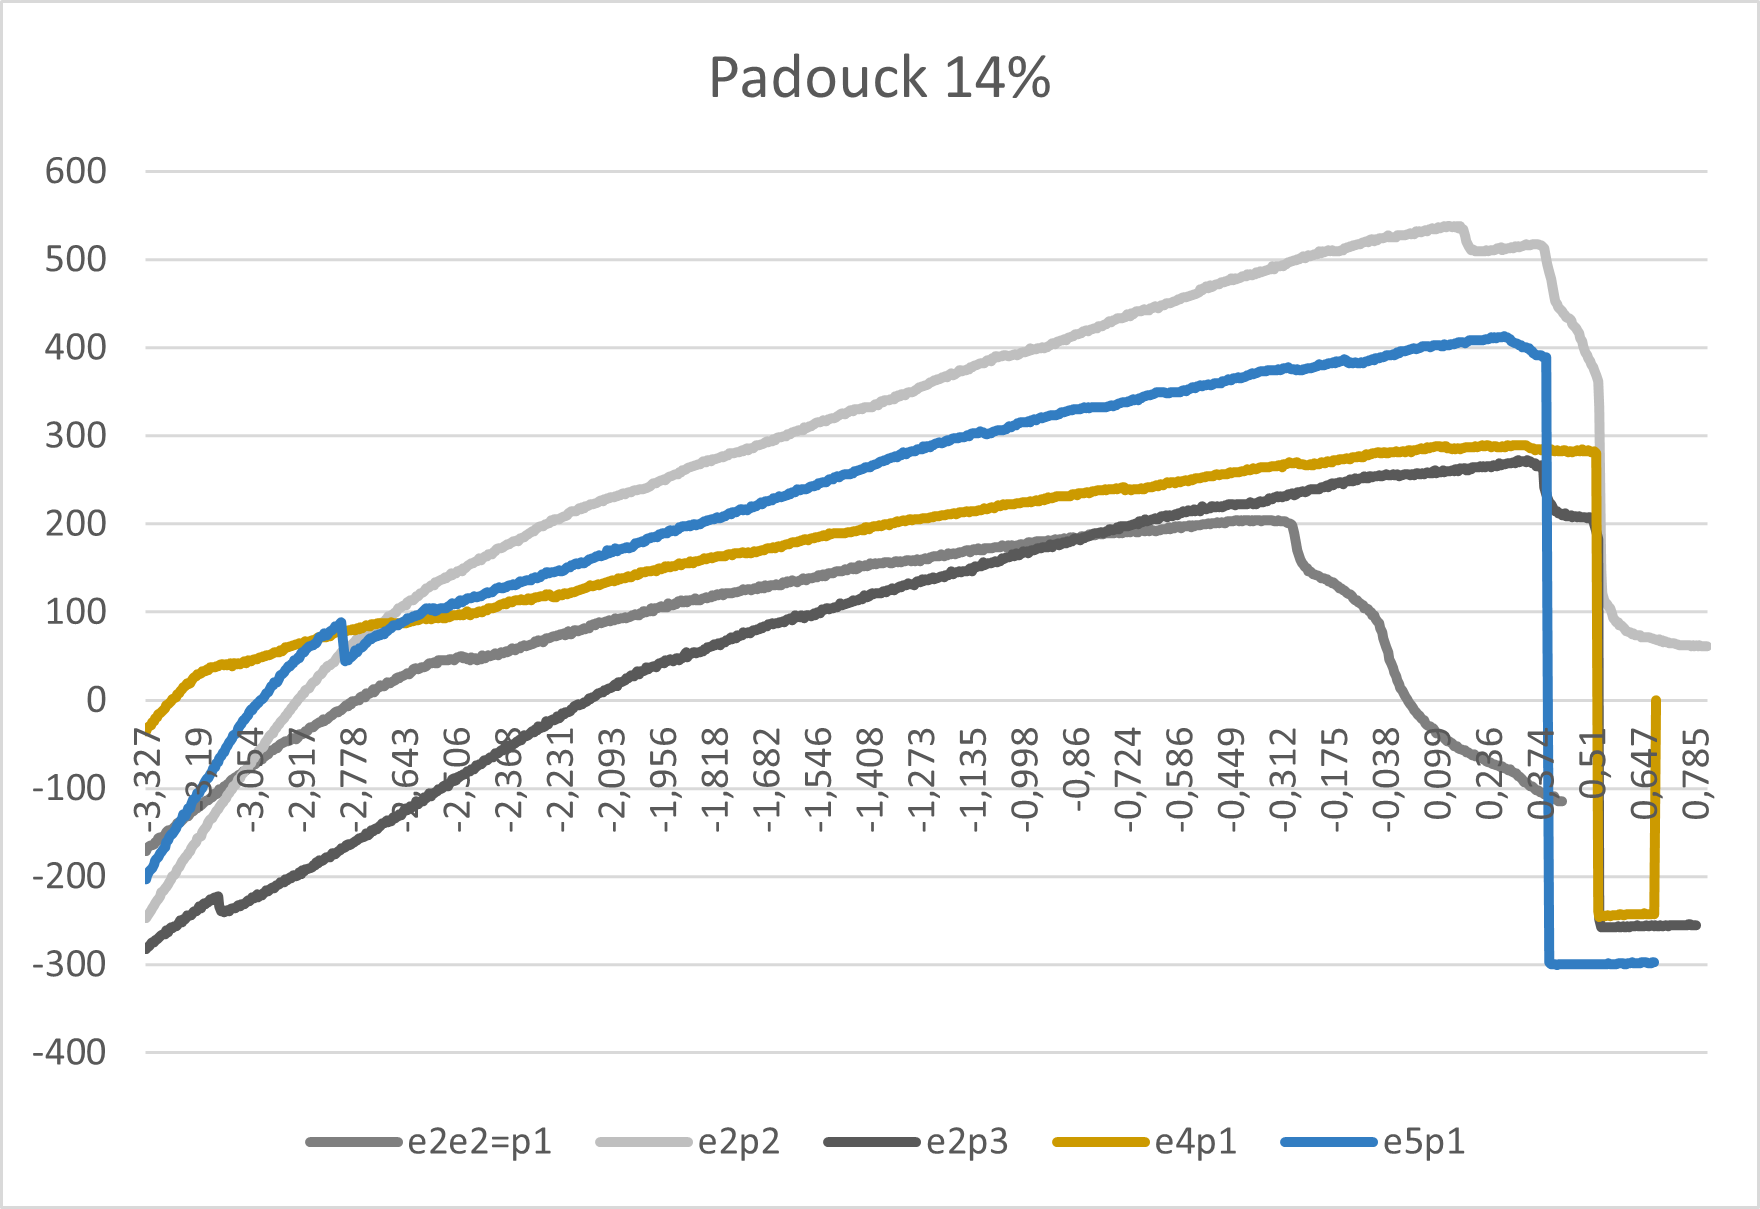
\includegraphics[scale=0.5]{Figures/PDelt_PAD14}
		\decoRule
		\caption[Padouk specimens tested at 14\% moisture content]{P-$\delta$ curves of Padouk specimens tested at a moisture content around 14\%}
		\label{fig:MC_Pad_14}
	\end{subfigure}
	\caption{P-$\delta$ curves at 20\% MC}
	\label{fig:Pdel_20_MC}
\end{figure}

The experiments were the last done. Indeed, the MC takes more time to decrease and reach 20\% than for E3 experiment. And many defaults were visible on the specimens expected for this test. For instance, even if the washers' solution was found, the E2O1 specimen was closed to the fixation hole rupture. Indeed, a little defect coupled with the important load applied on the heel, involve a propagation of this other crack. 

The cracks length evolution are shown in \ref{E2o_G} and \ref{E2p_G}. Of course, due to the different precracks and notches, it is not relevant to comment the last values of these curves. But the shapes and the necessary displacement to collapse the specimens are interesting. Considering alpha parameter as the best one possible to choose, plots as the E2P3 one \ref{fig:E2P3_a} is not an expected one. It presents a quick crack happening early in terms of displacement value, and comparing to others tested specimens. This kind of curve do not augur good G results. And regarding \ref{E2o_G} and \ref{E2p_G} graph, it is obvious that E2P3 behavior is not as interesting as the others. There are no evolution, just one step linked to the crack length evolution.

\begin{figure}[th]
	\centering
	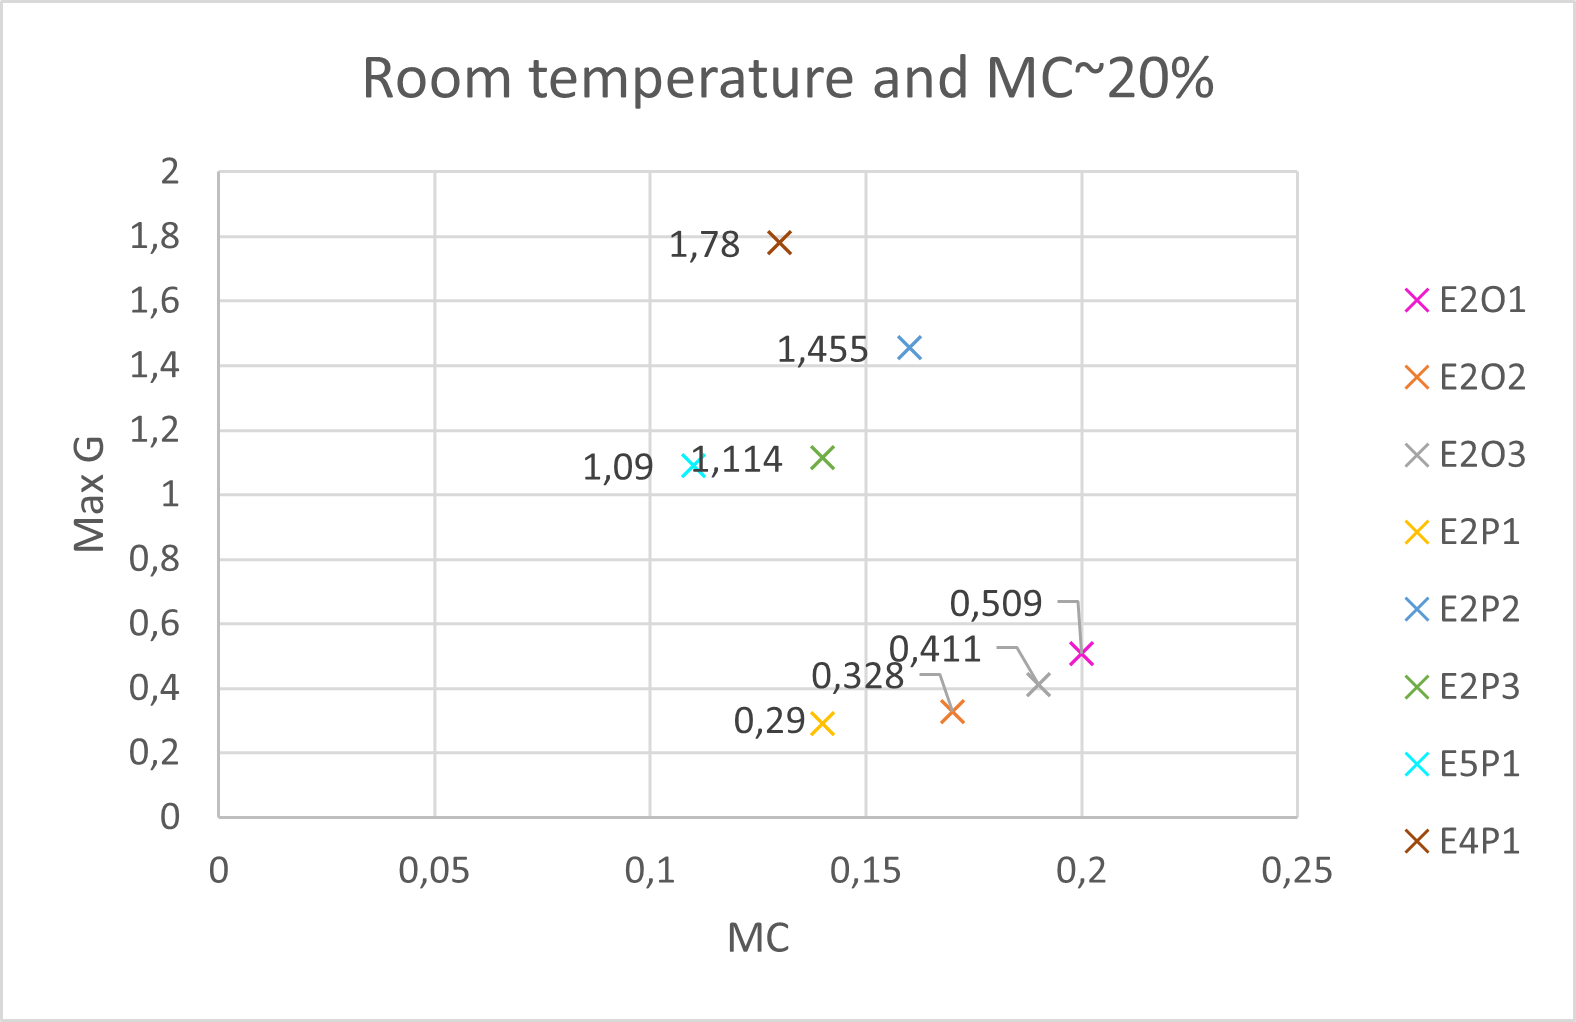
\includegraphics[width=\textwidth]{Figures/Res_MC20}
	\caption[G depending on MC for specimen at 20\%]{Energy release rate from tested specimen depending on MC for specimen at 20\%}
	\label{fig:Res_MC20}
\end{figure}

Even if E2O1 specimen as defects as mentioned before, maximal Okoume specimen G is reached by this sample. It should be logical to have a lower value for this specimen on \ref{fig:Res_MC20}. Indeed, all the energy was not used to increase the crack length in the ZOI, because a part of this energy was been creating a second crack. This is one of the difficulties by working on wood. A living material with a behavior changing between specimens made from the same tree does not allow a certain interpretation.

The cohesive laws from these experiments shows good shapes, compared to \parencite{Reference14} work for instance. The purpose of this curve is also to have a look on the area. $G_{critical}$ should be equal to the value of this area, under the curve. It is also important to notice that all the plots presenting G as a function of $w_{I}$ were created in order to have a look on the shape. It is expected to obtain a logistic curve shape. In this case of the second experiment, specimens as E2P2 or E2P3 \ref{RCexample} allow to have this logistic curve estimation.

\begin{figure}[h]
	\centering
	\begin{subfigure}{0.48\linewidth}
		\centering
		\includegraphics[scale=0.5]{Figures/characteristicR–curves_e2p2}
		\decoRule
		\caption[characteristic R–curves before cohesive law ploting E2P2]{characteristic R–curves of E2P2 specimen test}
		\label{fig:RcE2P2}
	\end{subfigure}
	\hfill
	\begin{subfigure}{0.48\linewidth}
		\includegraphics[scale=0.5]{Figures/characteristicR–curves_e2p3}
		\decoRule
		\caption[characteristic R–curves before cohesive law ploting E2P3]{characteristic R–curves of E2P3 specimen test}
		\label{fig:RcE2P3}
	\end{subfigure}
	\caption{characteristic R–curves shapes}
	\label{RCexample}
\end{figure}

Even if the shapes do not represent a perfect logistic curve, the cohesive laws from these R-curves shown on \ref{fig:E2P2_colaw} and \ref{fig:E2P3_colaw} gives coherent results even if the E3P3 specimen does not have an expected decrease. The E3P2 specimen is the perfect example to present the expected results, even if the plot of G depending on the crack length have a non common last value.

\newpage

%----------------------------------------------------------------------------------------
%	SUBSECTION 3
%----------------------------------------------------------------------------------------
\subsection{Results with specimen at a moisture content around 30\% }

The first values obtained on these tests were the ones given by the hydraulic press. The graph representing the R-curve, gives low load values for Padouck specimens, and the cracks occurs fast. But the final P-$\delta$ curves computed by Python as on \ref{E3p_Pdel} do not show real problems. Even the values are in a coherent range.

\begin{figure}[th]
	\centering
	\includegraphics[scale=0.8]{Figures/E3p_Pdel}
	\caption[P-$\delta$ curves for specimen at 30\%]{P-$\delta$ curves from experiment 3 specimens, tested at approximately 30\%}
	\label{E3p_Pdel}
\end{figure}

An interesting point from the P-$\delta$ curves, is the intermediary decrease visible in particular on E3P1 or E3O2 specimens. To link these events to experimental observation, it is due to a first crack propagation and also a crack tip opening displacement. During the specimen collapse, as explain before, bridges appears in the crack tip. It is shown on \ref{fig:Res_bridges}, with material linking both sides of the crack. This penomenom can be discussed, because the bridges do not allow a linear propagation. When they break, a gap occurs. The necessary load to carry on opening the crack tip is lower and it is involving the curve drops. 
\begin{figure}[th]
	\centering
	\includegraphics[width=\textwidth]{Figures/crack_bridges}
	\caption[Crack bridges]{Wood bridges between both sides of the crack}
	\label{fig:Res_bridges}
\end{figure}
But these bridges can involve false analysis. Indeed, the CTOD, $w_{I}$ will be more important if the bridges were not formed. While the crack length is still increasing, as visible on \ref{fig:Res_bridges}, with the crack tip position far from the last bridge. G is defined by a(t), but also by P (the load) which is a parameter affected by the bridges, and also C, depending itself on P. So G values are calculated with parameters, not affected by the same phenomenon.

Regarding a(t) values for this third experiment, no patterns can be easily presented. The curves shown on \ref{E3o_a} and \ref{E3p_a} have different shapes. For all the specimens, except the E3P2, the crack length exceed the ZOI. But the following energy release rate graphs, \ref{fig:Res_MC30}, \ref{E3o_G} and \ref{E3p_G} gives many information. 
First, the values from Okoume specimens are close even if a strange increasement pic occurs on E4O1 plot. The G maximal value is around 0.38\si{\newton\per\milli\meter} for this species at 30\% MC. For the Padouck values, the E3P3 looks like a false one. One interpretation done was linked to the long precrack. It has a 24.6\si{\milli\meter} precrack while E3P1 has a 21.9\si{\milli\meter} and E3P2 a precreack of 20.5\si{\milli\meter}. Even if this parameter is token in account for G determination, by subtracting the $a_{0}$ from the crack length, it also occurs a faster collapse, because a longer part of the specimen is already collapsed.
\begin{figure}[th]
	\centering
	\includegraphics[width=\textwidth]{Figures/Res_MC30}
	\caption[G depending on MC for specimen at 30\%]{Energy release rate from tested specimen depending on MC for specimen at 30\%}
	\label{fig:Res_MC30}
\end{figure}
The G graphs and the cohesive laws for these experiments are the ones with expected curves, even if results can be discussed. Even the shapes can be better, the G values do not reach a real plateau, the cohesive laws do not always decrease until first value, and the top of the curve looks more as a pic than as a real curve. But the approximate $\sigma$ have sometimes as \ref{E3o_colaw} too law values to be true ones. 

To conclude on these data, they look like made of too many approximations which will be discussed in the next part. Indeed, looking to \ref{tab:ArticleResult} and \parencite{Reference7}, G values should not reach 1.9\si{\newton\per\milli\meter} and be under 0.4\si{\newton\per\milli\meter} while it this case for many specimens. Likewise, the cohesive laws obtained must not be under 1\si{\mega\pascal}

%	\centering
%	\begin{subfigure}{0.48\linewidth}
%		\centering
%		\includegraphics[scale=0.5]{Figures/PDelt_OK27}
%		\decoRule
%		\caption[Okoume specimens tested at 27\% moisture content]{P-$\delta$ curves of Okoume specimens tested at a moisture content around 27\%}
%		\label{fig:MC_Ok_27}
%	\end{subfigure}
%	\hfill
%	\begin{subfigure}{0.48\linewidth}
%		\includegraphics[scale=0.5]{Figures/PDelt_PAD19}
%		\decoRule
%		\caption[Padouk specimens tested at 19\% moisture content]{P-$\delta$ curves of Padouk specimens tested at a moisture content around 19\%}
%		\label{fig:MC_Pad_19}
%	\end{subfigure}
%	\caption{P-$\delta$ curves at ambiant MC}
%	\label{Pdel_30_MC}
%\end{figure}
%
%\begin{figure}[th]
%	\centering
%	\includegraphics[scale=0.4]{Figures/e3o1_a}
%	\caption[crack length evolution depending on hydraulic press displacement]{crack length evolution depending on hydraulic press displacement.}
%	\label{fig:e3o1_a}
%\end{figure}

%----------------------------------------------------------------------------------------
%	SECTION 3
%-----------------------------------------------------------------------------$ -----------
\section{Data Analysis treatments and comparisons}
\begin{table}[H]
	\centering
	\begin{tabular}{c c c c}
		\hline
		\rowcolor[HTML]{F4B084} 
		\multicolumn{4}{c}{\cellcolor[HTML]{F4B084}room temperature and room MC} \\ 
		\rowcolor[HTML]{FCE4D6} 
		Name of the specimen & Max G & Max Load & MC \\
		\rowcolor[HTML]{FFFFFF} 
		E1O1 & 0,323 N/mm & 178 N & 7\% \\
		\rowcolor[HTML]{FFFFFF} 
		E102 & 0,412 N/mm & 158 N & 7\% \\
		\rowcolor[HTML]{FFFFFF} 
		E103 & 0,435 N/mm & 178 N & 7\% \\
		\rowcolor[HTML]{FFFFFF} 
		E1P1 & 0,195 N/mm & 176 N & 5\% \\
		\rowcolor[HTML]{FFFFFF} 
		E1P2 & 0,805 N/mm & 416 N & 5\% \\
		\rowcolor[HTML]{FFFFFF} 
		E1P3 & 0,477 N/mm & 321 N & 5\% \\
		\rowcolor[HTML]{AEAAAA} 
		E1I1 &  &  & 16\% \\
		\rowcolor[HTML]{F4B084} 
		\multicolumn{4}{c}{\cellcolor[HTML]{F4B084}room temperature and MC$\sim$20\%} \\
		\rowcolor[HTML]{FCE4D6} 
		Name of the specimen & Max G & Max Load & MC \\
		\rowcolor[HTML]{FFFFFF} 
		E2O1 & 0,509 N/mm & 279 N & 20\% \\
		\rowcolor[HTML]{FFFFFF} 
		E2O2 & 0,328 N/mm & 259 N & 17\% \\
		\rowcolor[HTML]{FFFFFF} 
		E2O3 & 0,411 N/mm & 290 N & 19\% \\
		\rowcolor[HTML]{FFFFFF} 
		E2P1 & 0,29 N/mm & 376 N & 14\% \\
		\rowcolor[HTML]{FFFFFF} 
		E2P2 & 1,455 N/mm & 785 N & 16\% \\
		\rowcolor[HTML]{FFFFFF} 
		E2P3 & 1,114 N/mm & 554 N & 14\% \\
		\rowcolor[HTML]{F4B084} 
		\multicolumn{4}{c}{\cellcolor[HTML]{F4B084}room temperature and MC$\sim$30\%} \\
		\rowcolor[HTML]{FCE4D6} 
		Name of the specimen & Max G & Max Load & MC \\
		\rowcolor[HTML]{FFFFFF} 
		E3O1 & 0,341 N/mm & 207 N & 24\% \\
		\rowcolor[HTML]{FFFFFF} 
		E3O2 & 0,378 N/mm & 195 N & 28\% \\
		\rowcolor[HTML]{FFFFFF} 
		E3O3 & 0,478 N/mm & 224 N & 27\% \\
		\rowcolor[HTML]{FFFFFF} 
		E3P1 & 0,993 N/mm & 536 N & 19\% \\
		\rowcolor[HTML]{FFFFFF} 
		E3P2 & 0,829 N/mm & 397 N & 19\% \\
		\rowcolor[HTML]{FFFFFF} 
		E3P3 & 0,441 N/mm & 481 N & 24\% \\
		\rowcolor[HTML]{F4B084} 
		\multicolumn{4}{c}{\cellcolor[HTML]{F4B084}Fridge samples} \\
		\rowcolor[HTML]{FCE4D6} 
		Name of the specimen & Max G & Max Load & MC \\
		\rowcolor[HTML]{FFFFFF} 
		E4O1 & 1,98 N/mm & 452 N & 31\% \\
		\rowcolor[HTML]{FFFFFF} 
		E4P1 & 1,78 N/mm & 535 N & 13\% \\
		\rowcolor[HTML]{AEAAAA} 
		E4I1 &  &  & 45\% \\
		\rowcolor[HTML]{F4B084} 
		\multicolumn{4}{c}{\cellcolor[HTML]{F4B084}Oven sample} \\
		\rowcolor[HTML]{FCE4D6} 
		Name of the specimen & Max G & Max Load & MC \\
		\rowcolor[HTML]{FFFFFF} 
		E5O1 & 0,17 N/mm & 176 N & 5\% \\
		\rowcolor[HTML]{FFFFFF} 
		E5P1 & 1,09 N/mm & 704 N & 11\% \\
		\rowcolor[HTML]{AEAAAA} 
		E5I1 &  &  & 29\% \\
	\end{tabular}
	\caption{Overview table of the maximal energy release rate and the maximal load}
	\label{tab:Recap_GandP}
\end{table}
The table \ref{tab:Recap_GandP} is a recap of the maximal values for G and P (load in Newton). It must be notified that this load values are the computed ones. It means that the shifting process was already done, and the data in kilo Newton, converted into Newton.
As it is reminded, all the MC reach are not similar and are classed into the expected categories of moisture content.

\newpage
%----------------------------------------------------------------------------------------
%	SUBSECTION 1
%----------------------------------------------------------------------------------------
\subsection{Comparison between species}

One of this work purpose was the comparison of different species. Indeed, as it is presented since the raw data chapter Iroko specimens do not give data, and Silver Fir specimens do not arrive at time to be tested. But the comparison is still done on a Padouck and Okoume which are species with different density, allowing interesting discussion. 

\ref{fig:Res_Pmax} presents all the specimens and the necessary loads to involve a propagation of the crack in all the ZOI and sometimes until the entire destruction of the specimen. The interest of the look on P-$\delta$ curves and in this case, the maximum P load is to avoid potential mistakes from post processing treatment. Even if the shown data are approximations due to the shifting process, it is less impacting that all the others approximations involve by the G determination.

\begin{figure}[th]
	\centering
	\includegraphics[width=\textwidth]{Figures/Res_Pmax}
	\decoRule
	\caption[Maximal load reach for each specimen]{Maximal load reach for each specimen compared to the Moisture Content of the specimens}
	\label{fig:Res_Pmax}
\end{figure}

As expected, Padouck specimens need a higher load to involve the final crack. It was obvious, that the denser material is more difficult to destroy than the lower one. Specimens as the E1P1 should not have load low values. It is quite difficult to find a logical reason to this kind of lower results. Indeed, the notch and precrack were not bigger than other ones, the MC is the same than in other Padouck specimens from the same test... 

Looking the MC impact on the tests, Okoume specimens seem to do not have the same behavior regarding to the Okoume point cloud. It looks like MC do not have impact on the Okoume behavior. At the opposite, Padouck appears to be affected by the humidity. A strange variation could be commented. It is one of the first time that values at a certain MC has a great impact on the wood material resistance. Indeed, at 20\% so around 15\% MC for Padouck specimens, values are increasing. It is significant regarding E2P2 specimen and relevant looking to E4P1, E5P1 or E2P3. Then the resistance of the material looks like decreasing by reaching a 25\% average of the MC. By looking closer to Okoume values, the same trend can be observed at a lower level. Indeed, Okoume load values around 20\% are higher than the ones tested in room conditions and also to the specimens with 30\% MC.

But looking to the high dispersion of the points, in particular for Padouck specimens, these theory should be discussed.

%----------------------------------------------------------------------------------------
%	SUBSECTION 2
%----------------------------------------------------------------------------------------
\subsection{Comparison between moisture content levels}

As shown before, the MC level affects wood behavior, it is still visible on \ref{fig:G_MC_species}. But here the trend is less visible.
\begin{figure}[th]
	\centering
	\includegraphics[width=\textwidth]{Figures/G_MC_species}
	\decoRule
	\caption[Energy release rate linked to species and moisture content]{Energy release rate linked to species and moisture content}
	\label{fig:G_MC_species}
\end{figure}

Indeed, Okoume specimens look more constant and the impact of MC on the behavior is not really characterized. 
This results must be criticize and another way to compare the results, is also to have a look at the CTOD values depending on the servohydraulic test machine. By a comparison of the CTOD regarding the MC present into the specimens, others conclusions can be done. To comment this graphs \ref{fig:Res_CTOD_o} and \ref{fig:Res_CTOD_o}, a previous observation can be done again, the Padouk, more fragile, break for some specimens before 1.5\si{\milli\meter} of displacement. Indeed, as said before, Padouk specimens have a quick crack propagation. The crack length evolves more elastically for Okoume specimens, and allow a better study. It is important to notes that the values at 0 are linked to the end of the test, and the too high value of the CTOD. As explain in the post processing computation, the pair of subsets chosen give the main information, but at a certain level, they are into the crack and are considered as NaN values or 0. This problem can be solved by using other pair of subsets, but the curve shape could be different as presented in \ref{fig:CODpairchos}
\newpage
\begin{sidewaysfigure}
%\begin{figure}[h]
	\centering
	\includegraphics[width=\textwidth]{Figures/Res_CTOD_o}
	\decoRule
	\caption[CTOD and MC on Okoume specimens]{Crack Tip Opening Displacements and MC on Okoume specimens depending on the displacement from the hydraulic press}
	\label{fig:Res_CTOD_o}
\end{sidewaysfigure}
\newpage
\begin{sidewaysfigure}
	\centering
	\includegraphics[width=\textwidth]{Figures/Res_CTOD_p}
	\decoRule
	\caption[CTOD and MC on Padouck specimens]{Crack Tip Opening Displacements and MC on Padouck specimens depending on the displacement from the hydraulic press}
	\label{fig:Res_CTOD_p}
%	\caption[CTOD analysis]{Crack Tip Opening Displacements linked to MC and displacement}
%	\label{Res_CTOD}
%\end{figure}
\end{sidewaysfigure}
In \ref{fig:Res_CTOD_o} almost all the specimens do not have a CTOD higher than 0.8\si{\milli\meter}, due to the collapse at 1.5\si{\milli\meter} or 1.7\si{\milli\meter} of hydraulic press displacement. Only 3 specimens do not follow this trend, E3P1, E2P2 and E1P1. It is interesting to identify the specimens with bigger CTOD values. The 3 specimens are from tests carry out at different MC. So it can be a proof that the MC does not affect Padouck crack tip opening displacement. Regarding the Okoume specimens, it seems that the MC can have an impact. By avoiding the analysis of E3O1 at 24\% and E5O1 at 5\% it is possible to consider that the increase of the MC involve a higther CTOD values. Indeed, at 27\% and 28\% specimens CTOD exceed 1.4\si{\milli\meter}. Even if the values of the CTOD for Padouck specimen look like to increase too, the point cloud do not allow to conclude. A variation of 0.2\si{\milli\meter} between specimens at 5\% and those at 20\% exists, it is a too low delta, and specimen exceptions do not allow to compared average. This is the case on G values and on cohesive laws also.

So again, even by looking to the CTOD more than on the previous presented plots as G or the cohesive law, no real trend are found. Reading the literature, it was expected a decrease of the Energy release rate and a lower $\sigma$ value to involve the critical crack. But this tendency was not as visible as predicted.   


%----------------------------------------------------------------------------------------
%	SUBSECTION 3
%----------------------------------------------------------------------------------------
\subsection{Differences with previous works}

A lot of differences are found with previous works. Indeed, the works on this MMCG geometry, as in \parencite{Reference7} and in \parencite{Reference8} works, show different results. \parencite{Reference8} present similar results to the ones visible in this work, but with other species than the one presented here. While results in \parencite{Reference7} works are lower in terms of Energy release rate obtained. Indeed, Okoume specimens reached 2\si{\joule\per\square\meter} while our maximum results are around 400\si{\joule\per\square\meter}.

Indeed a quick conversion as the one explained below allow to compare our results to the ones from others articles.
1\si{\joule}=1\si{\kilo\gram\square\meter\per\square\second}
and 1\si{\newton}=1\si{\kilo\gram\meter\per\square\second}, so with the current results presented in  \si{\newton\per\milli\meter} they will be converted to \num{e3}\si{\joule\per\square\meter} 
The only values which make sense with ones presented in this work, are the ones from \parencite{Ang2017} studies. Indeed Douglas Fir specimens with a density between Padouck and Okoume, reach G values between ours. Indeed, it is included between 780\si{\joule\per\square\meter} at 9\% MC and 680\si{\joule\per\square\meter} at 18\% MC.

The interesting point is the new trend presenting in this analysis. Indeed the Silver Fir was one of the first material to whom, the increase of MC involves an increase of G. It is the case in \parencite{Ang2017} or \parencite{Huang2020} for instance. But considering the previous results as operable data, by looking on more than 2 MC, the behavior of the material looks different. In every works the MC increase phenomenon decrease the Resistance of the material. The G and the $\sigma$ were obtained on European species and this trend was confirmed. But since the beginning of tests on Tropical species, others behavior are found. \parencite{Reference7} has proved by his work, that the results, regarding to the mode and the load angle applied, for Iroko, Okoume and Padouck, are similar to European ones. But no proof were already done concerning the behavior of this species to MC effect. This species from Gabon are submitted to higher temperature and relative humidity around 80\%. And looking to work as \parencite{Kif1998} and \parencite{Ang2017}, the density of Scots Pine and Douglas, can be compared to Okoume specimens, and then the results from these specimens can be discussed. It appears that the early wood more saturated in water than the lately one involves a decrease of the $\sigma$. A similar trend is shown on Douglas Fir regarding two MC values, 9\% and 18\%. The fact is that the Okoume species do not have this trend and is stable. The difficulties to well interpret these results come also from the cohesive laws values as \ref{fig:E1O1_colaw} and \ref{fig:E1O3_colaw} compared to \ref{fig:E2O1_colaw} and \ref{fig:E2O2_colaw}. On these plots the trend can be confirmed, but the values are too far from those presented on Scots Pine by \parencite{Huang2020} which show a $\sigma$ parameter about 36\si{\mega\pascal} for resoaked specimens. In another hand, the Jack Pines values at 2\% were around 4.5\si{\mega\pascal} while Okoume specimen submitted at room conditions reach 14\si{\mega\pascal} or almost 25\si{\mega\pascal}.

In conclusion,the results from the cohesive laws look like false one in comparison to previous work. Indeed, except the cited ones, a lot of the plotted cohesive laws have values below 1\si{\mega\pascal} which should not be the case. Looking to the G values, they could be compared as shown with \parencite{Ang2017} work. But the absence of trend as previous ones is questioning. This is a way to discuss about the results found for parameters as $w_{I}$ and G which involve strange cohesive laws and difficult curves to analyze.
%----------------------------------------------------------------------------------------
%	SUBSECTION 4
%----------------------------------------------------------------------------------------
\subsection{Way of amelioration and next step}

As it is visible, no real conclusion can be made looking to these results. But the work can be carry on and many amelioration can be added. Except the ones presented in the difficulties and issues chapter, experimental improvement exists. 

The specimens must be well controlled in term of shapes, composition and preparation. Indeed, even if the formulas and experiments take care of the thickness, the precrack and all these parameters measured by ourselves, are important approximation. Moreover, by having all these parameters modifications, it increases the analysis complexity.

One of the main problems from this work was also the raw data from the servohydraulic press device. Indeed as explained, a shift was applied on the P-$\delta$ to avoid the negative values which do not have sense. But by adding this shift, a choice was made to do not take into account the preload. Indeed, to avoid the movement of the specimen, it was loaded before the camera adjustment to be sure that the ZOI will be well focused. This preload on some specimens can reach 100\si{\newton}, so by ignoring this first loading process, every result are truncated and the impacts on others parameters are disastrous. The P load, is necessary to compute the Compliance and the Energy release rate, so by using false values it affects those resultants. G is particularly impacted due to the square factor affected to the load parameter. This problem could explain the weird values obtained for G. To provide this problem, it is necessary to have a look to the hydraulic press load before the beginning of its used. This value, even if it is a negative one, will be subtracted to each other one, allowing to have the preload. Another solution is to carry on the tests, even after the end of the propagation into the ZOI. Indeed, the load value at the end of the test, on a collapsed specimen will be at zero, even if the zero value is a negative one. 

Looking to post processing amelioration, an optimization of the crack length determination can be done. Indeed, the shapes of the a(t) evolution graphs are realistic but involves strange shapes for G plots. In the experimental work, it was visible that the crack reach a step, stabilize the propagation until the bridges break and reach another step. And this is what the Python code succeed to compute. But these steps do not permit a smooth plot of the G parameter. A solution can be to compute a least square curve to avoid the steps. It also allows to compare different methods in order to compute G. Indeed, it was tackled to use the compliance as a derivative function, derivated by the crack length as explained before. It could be easily computed if the crack length has a smoother shape, allowing to easily obtained the intersection and the slope. It was defined that the finite difference could help to obtain these shapes. 

This work, which concerns a large subject, can be used to work on tinnier and more precise works. Indeed, it was not possible to finalize the comparison with Abaqus software. But looking to the cohesive laws and all the data obtained in this Research and Developpement Project, the comparison could allow a better understanding of wood behavior, depending on Moisture Content. In the same way, this work had the objective to compare different climatic impact on wood behavior. It could be interesting to realize these expected experiments at different temperature and also with Fatigue Load. The last improvement should be the real comparison with an European species. The behavior should change and the impact of the MC could be different looking to the climatic differences in the growth area of the trees chosen to be tested. 

Then, this work could also be pushed and the same experimental process can be used again to observed wood behavior submitted to a Mode II or Mode III solicitation. Arcan grips are already designed and all the material is available at FCT university. Moreover, this work was a first step in wood fracture mechanics analysis at FCT Mechanical department. Looking to this problems, they can be solved for next experiments.


% Chapter Template

\chapter{Conclusion} % Main chapter title

\label{Conclusion} % Change X to a consecutive number; for referencing this chapter elsewhere, use \ref{ChapterX}

%----------------------------------------------------------------------------------------
%	SECTION 1
%----------------------------------------------------------------------------------------

In conclusion of this work, by analyzing the behavior of Padouk and Okoume species submitted to different moisture content, this study has shown how this climatic effect can affect wood fracture mechanics.
\newline
The tests done at different moisture contents, climatic room, 20\% and 30\%, for several MMCG geometry specimens, coupled to the use of DIC with MatchID software and python processing were determinant to obtained results. Even if the final experiments do not present tests at changing temperature or the specimen collapsed by fatigue loads, the focus was put on moisture content parameter, allowing to have more samples to treat, in order to have a better idea of a potential trend. The choice of the focus on this parameter more than others, was linked to the little research done on this parameter while numerous are leaded on temperature variation and fatigue impact. Whereas, the Silver Fir was not able to be treated, so the experiments do not compare tropical species with temperate ones. But a comparison was done on previous work. 
The link between European species and Okoume in terms of density show a difference of behavior. Okoume looks like a less affected wood regarding moisture content impact on its mechanical characteristics. At the contrary, the final trend visible on the Padouck available results, was not compared with european species, due to the absence of fracture mechanic tests at different moisture content for this denser wood. So the results shown and the interpretation can be discussed, but according to this work, Padouck seems to have better characteristics at 15\% moisture content, before a decrease of the energy release rate with the 20\% moisture content treeshold overrun. 
\newline
The impossibility to do real comparison due to the shapes of the samples, the species and the moisture content variation, intrinsic to this project, does not allow a final answer. But the uses of this work are numerous. Some issues were found and solutions are proposed to avoid future problems on the test. By changing one parameter as the moisture content or the species, it will be possible to reuse the developed Python code and many determined parameters, in order to find a pattern linking moisture content to fracture mechanics in mode 1. An obvious conclusion is that wood behavior is submitted to too many evolution to found an empiric model, and every specimen tested will be a particular case. This is the reason why much experiments must be done on this exceptional material.

%----------------------------------------------------------------------------------------
%	BIBLIOGRAPHY
%----------------------------------------------------------------------------------------

\printbibliography[heading=bibintoc]

%----------------------------------------------------------------------------------------
%------------------------------
%	THESIS CONTENT - APPENDICES
%------------------------------

\begin{appendices} % Cue to tell LaTeX that the following "chapters" are Appendices

% Include the appendices of the thesis as separate files from the Appendices folder
% Uncomment the lines as you write the Appendices

% Appendix 1

\chapter{Results from Python computation} % Main appendix title

\label{Appendix1} % For referencing this appendix elsewhere, use \ref{AppendixA}

%%%%%%%%%%%%%%%%%%%%%%%%%%%%%%%%%%%%%%%%%%%%%%%%%
%Section 1
%%%%%%%%%%%%%%%%%%%%%%%%%%%%%%%%%%%%%%%%%%%%%%%%%

\section{Results in mode I for $\alpha=0 ^\circ$}

\subsection{e0e1}

\begin{figure}[H]
	\centering
	\begin{subfigure}{0.48\linewidth}
		\centering
		\includegraphics[width=\textwidth]{P_e0e1}
		\decoRule
		\caption{P-Delta curve, for e0e1 specimen.}
		\label{fig:P_e0e1}
	\end{subfigure}
	\hfill 
	\begin{subfigure}{0.48\linewidth}
		\centering
		\includegraphics[width=\textwidth]{a_e0e1}
		\decoRule
		\caption{Crack length depending on time, for e0e1 specimen.}
		\label{fig:a_e0e1}
	\end{subfigure}
	\hfill\\
	\begin{subfigure}{0.48\linewidth}
		\centering
		\includegraphics[width=\textwidth]{Gmet1_e0e1}
		\decoRule
		\caption{Energy release rate depending on the crack length propagation method 1, for e0e1 specimen.}
		\label{fig:Gmet1_e0e1}
	\end{subfigure}
	\hfill
	\begin{subfigure}{0.48\linewidth}
		\centering
		\includegraphics[width=\textwidth]{Gmet2_e0e1}
		\decoRule
		\caption{Energy release rate depending on the crack length propagation method 2, for e0e1 specimen.}
		\label{fig:Gmet2_e0e1}
	\end{subfigure}
	\caption{Mechanical fracture characteristics of specimen e0e1}
	\label{E1o_a}
\end{figure}

\subsection{e0e2}

\begin{figure}[H]
	\centering
	\begin{subfigure}{0.48\linewidth}
		\centering
		\includegraphics[width=\textwidth]{P_e0e2}
		\decoRule
		\caption{P-Delta curve, for e0e2 specimen.}
		\label{fig:P_e0e2}
	\end{subfigure}
	\hfill 
	\begin{subfigure}{0.48\linewidth}
		\centering
		\includegraphics[width=\textwidth]{a_e0e2}
		\decoRule
		\caption{Crack length depending on time, for e0e2 specimen.}
		\label{fig:a_e0e2}
	\end{subfigure}
	\hfill\\
	\begin{subfigure}{0.48\linewidth}
		\centering
		\includegraphics[width=\textwidth]{Gmet1_e0e2}
		\decoRule
		\caption{Energy release rate depending on the crack length propagation method 1, for e0e2 specimen.}
		\label{fig:Gmet1_e0e2}
	\end{subfigure}
	\hfill
	\begin{subfigure}{0.48\linewidth}
		\centering
		\includegraphics[width=\textwidth]{Gmet2_e0e2}
		\decoRule
		\caption{Energy release rate depending on the crack length propagation method 2, for e0e2 specimen.}
		\label{fig:Gmet2_e0e2}
	\end{subfigure}
	\caption{Mechanical fracture characteristics of specimen e0e2}
	\label{E1o_a}
\end{figure}

\subsection{e0e3}

\begin{figure}[H]
	\centering
	\begin{subfigure}{0.48\linewidth}
		\centering
		\includegraphics[width=\textwidth]{P_e0e3}
		\decoRule
		\caption{P-Delta curve, for e0e3 specimen.}
		\label{fig:P_e0e3}
	\end{subfigure}
	\hfill 
	\begin{subfigure}{0.48\linewidth}
		\centering
		\includegraphics[width=\textwidth]{a_e0e3}
		\decoRule
		\caption{Crack length depending on time, for e0e3 specimen.}
		\label{fig:a_e0e3}
	\end{subfigure}
	\hfill\\
	\begin{subfigure}{0.48\linewidth}
		\centering
		\includegraphics[width=\textwidth]{Gmet1_e0e3}
		\decoRule
		\caption{Energy release rate depending on the crack length propagation method 1, for e0e3 specimen.}
		\label{fig:Gmet1_e0e3}
	\end{subfigure}
	\hfill
	\begin{subfigure}{0.48\linewidth}
		\centering
		\includegraphics[width=\textwidth]{Gmet2_e0e3}
		\decoRule
		\caption{Energy release rate depending on the crack length propagation method 2, for e0e3 specimen.}
		\label{fig:Gmet2_e0e3}
	\end{subfigure}
	\caption{Mechanical fracture characteristics of specimen e0e3}
	\label{E1o_a}
\end{figure}

\subsection{e0e5}

\begin{figure}[H]
	\centering
	\begin{subfigure}{0.48\linewidth}
		\centering
		\includegraphics[width=\textwidth]{P_e0e5}
		\decoRule
		\caption{P-Delta curve, for e0e5 specimen.}
		\label{fig:P_e0e5}
	\end{subfigure}
	\hfill 
	\begin{subfigure}{0.48\linewidth}
		\centering
		\includegraphics[width=\textwidth]{a_e0e5}
		\decoRule
		\caption{Crack length depending on time, for e0e5 specimen.}
		\label{fig:a_e0e5}
	\end{subfigure}
	\hfill\\
	\begin{subfigure}{0.48\linewidth}
		\centering
		\includegraphics[width=\textwidth]{Gmet1_e0e5}
		\decoRule
		\caption{Energy release rate depending on the crack length propagation method 1, for e15e4 specimen.}
		\label{fig:Gmet1_e0e5}
	\end{subfigure}
	\hfill
	\begin{subfigure}{0.48\linewidth}
		\centering
		\includegraphics[width=\textwidth]{Gmet2_e0e5}
		\decoRule
		\caption{Energy release rate depending on the crack length propagation method 2, for e0e5 specimen.}
		\label{fig:Gmet2_e0e5}
	\end{subfigure}
	\caption{Mechanical fracture characteristics of specimen e0e5}
	\label{E1o_a}
\end{figure}

\subsection{e0e6}

\begin{figure}[H]
	\centering
	\begin{subfigure}{0.48\linewidth}
		\centering
		\includegraphics[width=\textwidth]{P_e0e6}
		\decoRule
		\caption{P-Delta curve, for e0e6 specimen.}
		\label{fig:P_e0e6}
	\end{subfigure}
	\hfill 
	\begin{subfigure}{0.48\linewidth}
		\centering
		\includegraphics[width=\textwidth]{a_e0e6}
		\decoRule
		\caption{Crack length depending on time, for e0e6 specimen.}
		\label{fig:a_e0e6}
	\end{subfigure}
	\hfill\\
	\begin{subfigure}{0.48\linewidth}
		\centering
		\includegraphics[width=\textwidth]{Gmet1_e0e6}
		\decoRule
		\caption{Energy release rate depending on the crack length propagation method 1, for e0e6 specimen.}
		\label{fig:Gmet1_e0e6}
	\end{subfigure}
	\hfill 
	\begin{subfigure}{0.48\linewidth}
		\centering
		\includegraphics[width=\textwidth]{Gmet2_e0e6}
		\decoRule
		\caption{Energy release rate depending on the crack length propagation method 2, for e0e6 specimen.}
		\label{fig:Gmet2_e0e6}
	\end{subfigure}
	\caption{Mechanical fracture characteristics of specimen e0e6}
	\label{E1o_a}
\end{figure}



\section{Results in mixed mode for $\alpha=15 ^\circ$}

\subsection{e15e1}

\begin{figure}[H]
	\centering
\begin{subfigure}{0.48\linewidth}
	\centering
	\includegraphics[width=\textwidth]{P_e15e1}
	\decoRule
	\caption{P-Delta curve, for e15e1 specimen.}
	\label{fig:P_e15e1}
\end{subfigure}
\hfill \\
\begin{subfigure}{0.48\linewidth}
	\centering
	\includegraphics[width=\textwidth]{a_e15e1}
	\decoRule
	\caption{Crack length depending on time, for e15e1 specimen.}
	\label{fig:a_e15e1}
\end{subfigure}
\hfill\\
\begin{subfigure}{0.48\linewidth}
	\centering
	\includegraphics[width=\textwidth]{G_e15e1}
	\decoRule
	\caption{Energy release rate depending on the crack length propagation, for e15e1 specimen.}
	\label{fig:G_e15e1}
\end{subfigure}
\caption{Mechanical fracture characteristics of specimen e15e1}
\label{E1o_a}
\end{figure}

\subsection{e15e2}

\begin{figure}[H]
	\centering
	\begin{subfigure}{0.48\linewidth}
		\centering
		\includegraphics[width=\textwidth]{P_e15e2}
		\decoRule
		\caption{P-Delta curve, for e15e2 specimen.}
		\label{fig:P_e15e2}
	\end{subfigure}
	\hfill \\
	\begin{subfigure}{0.48\linewidth}
		\centering
		\includegraphics[width=\textwidth]{a_e15e2}
		\decoRule
		\caption{Crack length depending on time, for e15e2 specimen.}
		\label{fig:a_e15e2}
	\end{subfigure}
	\hfill\\
	\begin{subfigure}{0.48\linewidth}
		\centering
		\includegraphics[width=\textwidth]{G_e15e2}
		\decoRule
		\caption{Energy release rate depending on the crack length propagation, for e15e2 specimen.}
		\label{fig:G_e15e2}
	\end{subfigure}
	\caption{Mechanical fracture characteristics of specimen e15e2}
	\label{E1o_a}
\end{figure}

\subsection{e15e3}

\begin{figure}[H]
	\centering
	\begin{subfigure}{0.48\linewidth}
		\centering
		\includegraphics[width=\textwidth]{P_e15e3}
		\decoRule
		\caption{P-Delta curve, for e15e3 specimen.}
		\label{fig:P_e15e3}
	\end{subfigure}
	\hfill \\
	\begin{subfigure}{0.48\linewidth}
		\centering
		\includegraphics[width=\textwidth]{a_e15e3}
		\decoRule
		\caption{Crack length depending on time, for e15e3 specimen.}
		\label{fig:a_e15e3}
	\end{subfigure}
	\hfill\\
	\begin{subfigure}{0.48\linewidth}
		\centering
		\includegraphics[width=\textwidth]{G_e15e3}
		\decoRule
		\caption{Energy release rate depending on the crack length propagation, for e15e3 specimen.}
		\label{fig:G_e15e3}
	\end{subfigure}
	\caption{Mechanical fracture characteristics of specimen e15e3}
	\label{E1o_a}
\end{figure}

\subsection{e15e4}

\begin{figure}[H]
	\centering
	\begin{subfigure}{0.48\linewidth}
		\centering
		\includegraphics[width=\textwidth]{P_e15e4}
		\decoRule
		\caption{P-Delta curve, for e15e4 specimen.}
		\label{fig:P_e15e3}
	\end{subfigure}
	\hfill \\
	\begin{subfigure}{0.48\linewidth}
		\centering
		\includegraphics[width=\textwidth]{a_e15e4}
		\decoRule
		\caption{Crack length depending on time, for e15e4 specimen.}
		\label{fig:a_e15e4}
	\end{subfigure}
	\hfill\\
	\begin{subfigure}{0.48\linewidth}
		\centering
		\includegraphics[width=\textwidth]{G_e15e4}
		\decoRule
		\caption{Energy release rate depending on the crack length propagation, for e15e4 specimen.}
		\label{fig:G_e15e4}
	\end{subfigure}
	\caption{Mechanical fracture characteristics of specimen e15e4}
	\label{E1o_a}
\end{figure}

\subsection{e15e5}

\begin{figure}[H]
	\centering
	\begin{subfigure}{0.48\linewidth}
		\centering
		\includegraphics[width=\textwidth]{P_e15e5}
		\decoRule
		\caption{P-Delta curve, for e15e5 specimen.}
		\label{fig:P_e15e5}
	\end{subfigure}
	\hfill \\
	\begin{subfigure}{0.48\linewidth}
		\centering
		\includegraphics[width=\textwidth]{a_e15e5}
		\decoRule
		\caption{Crack length depending on time, for e15e5 specimen.}
		\label{fig:a_e15e5}
	\end{subfigure}
	\hfill\\
	\begin{subfigure}{0.48\linewidth}
		\centering
		\includegraphics[width=\textwidth]{G_e15e5}
		\decoRule
		\caption{Energy release rate depending on the crack length propagation, for e15e5 specimen.}
		\label{fig:G_e15e5}
	\end{subfigure}
	\caption{Mechanical fracture characteristics of specimen e15e5}
	\label{E1o_a}
\end{figure}



\section{Results in mixed mode for $\alpha=30 ^\circ$}

\subsection{e30e2}

\begin{figure}[H]
	\centering
	\begin{subfigure}{0.48\linewidth}
		\centering
		\includegraphics[width=\textwidth]{P_e30e2}
		\decoRule
		\caption{P-Delta curve, for e15e1 specimen.}
		\label{fig:P_e30e2}
	\end{subfigure}
	\hfill \\
	\begin{subfigure}{0.48\linewidth}
		\centering
		\includegraphics[width=\textwidth]{a_e30e2}
		\decoRule
		\caption{Crack length depending on time, for e15e1 specimen.}
		\label{fig:a_e30e2}
	\end{subfigure}
	\hfill\\
	\begin{subfigure}{0.48\linewidth}
		\centering
		\includegraphics[width=\textwidth]{G_e30e2}
		\decoRule
		\caption{Energy release rate depending on the crack length propagation, for e15e1 specimen.}
		\label{fig:G_e30e2}
	\end{subfigure}
	\caption{Mechanical fracture characteristics of specimen e30e2}
	\label{E1o_a}
\end{figure}

\subsection{e30e3}

\begin{figure}[H]
	\centering
	\begin{subfigure}{0.48\linewidth}
		\centering
		\includegraphics[width=\textwidth]{P_e30e3}
		\decoRule
		\caption{P-Delta curve, for e30e3 specimen.}
		\label{fig:P_e30e3}
	\end{subfigure}
	\hfill \\
	\begin{subfigure}{0.48\linewidth}
		\centering
		\includegraphics[width=\textwidth]{a_e30e3}
		\decoRule
		\caption{Crack length depending on time, for e30e3 specimen.}
		\label{fig:a_e30e3}
	\end{subfigure}
	\hfill\\
	\begin{subfigure}{0.48\linewidth}
		\centering
		\includegraphics[width=\textwidth]{G_e30e3}
		\decoRule
		\caption{Energy release rate depending on the crack length propagation, for e30e3 specimen.}
		\label{fig:G_e30e3}
	\end{subfigure}
	\caption{Mechanical fracture characteristics of specimen e30e3}
	\label{E1o_a}
\end{figure}

\subsection{e30e5}

\begin{figure}[H]
	\centering
	\begin{subfigure}{0.48\linewidth}
		\centering
		\includegraphics[width=\textwidth]{P_e30e5}
		\decoRule
		\caption{P-Delta curve, for e30e5 specimen.}
		\label{fig:P_e30e5}
	\end{subfigure}
	\hfill \\
	\begin{subfigure}{0.48\linewidth}
		\centering
		\includegraphics[width=\textwidth]{a_e30e5}
		\decoRule
		\caption{Crack length depending on time, for e30e5 specimen.}
		\label{fig:a_e30e5}
	\end{subfigure}
	\hfill\\
	\begin{subfigure}{0.48\linewidth}
		\centering
		\includegraphics[width=\textwidth]{G_e30e5}
		\decoRule
		\caption{Energy release rate depending on the crack length propagation, for e30e5 specimen.}
		\label{fig:G_e30e5}
	\end{subfigure}
	\caption{Mechanical fracture characteristics of specimen e30e5}
	\label{E1o_a}
\end{figure}

\subsection{e30e7}

\begin{figure}[H]
	\centering
	\begin{subfigure}{0.48\linewidth}
		\centering
		\includegraphics[width=\textwidth]{P_e30e7}
		\decoRule
		\caption{P-Delta curve, for e30e7 specimen.}
		\label{fig:P_e30e7}
	\end{subfigure}
	\hfill \\
	\begin{subfigure}{0.48\linewidth}
		\centering
		\includegraphics[width=\textwidth]{a_e30e7}
		\decoRule
		\caption{Crack length depending on time, for e30e7 specimen.}
		\label{fig:a_e30e7}
	\end{subfigure}
	\hfill\\
	\begin{subfigure}{0.48\linewidth}
		\centering
		\includegraphics[width=\textwidth]{G_e30e7}
		\decoRule
		\caption{Energy release rate depending on the crack length propagation, for e30e7 specimen.}
		\label{fig:G_e30e7}
	\end{subfigure}
	\caption{Mechanical fracture characteristics of specimen e30e7}
	\label{E1o_a}
\end{figure}






%% Appendix 2

\chapter{Weight table presenting MC evolution} % Main appendix title

\label{Appendix2} % For referencing this appendix elsewhere, use \ref{AppendixA}

\section{Specimen preparation}

First, it was necessary to know the MC in the specimens submited at the ambiant humidity and temperature. \ref{tab:Tab3} present all the specimens weight at normal conditions, the potential difference invlves by scale changes and the MC obtained after drying the specimens.
\newpage
\begin {table}[h]
\centering
\begin{tabular}{r|c|c|c|c|r|}
	\hline
	\multicolumn{1}{|c|}{Name} & Weight [g] & Max   & Min   & Dry [g] & \multicolumn{1}{|c}{ambiant MC } \\
	\hline
	\hline
	\rowcolor[rgb]{ .675,  .725,  .792} \multicolumn{6}{|c|}{ambiant t° \& ambiant MC} \\
	\hline
	\hline
	\rowcolor[rgb]{ .973,  .796,  .678} \multicolumn{1}{|c|}{E1O1} & \multicolumn{1}{|c|}{\cellcolor[rgb]{ 1,  1,  1}43,6958} & \multicolumn{1}{|c|}{\cellcolor[rgb]{ 1,  1,  1}44,2637} & \multicolumn{1}{|c|}{\cellcolor[rgb]{ 1,  1,  1}43,1279} & \multicolumn{1}{|c|}{\cellcolor[rgb]{ 1,  1,  1}40,088} & \multicolumn{1}{|c|}{\cellcolor[rgb]{ 1,  1,  1}9,00\%} \\
	\hline
	\hline
	\rowcolor[rgb]{ .973,  .796,  .678} \multicolumn{1}{|c|}{E1O2} & \multicolumn{1}{|c|}{\cellcolor[rgb]{ 1,  1,  1}39,933} & \multicolumn{1}{|c|}{\cellcolor[rgb]{ 1,  1,  1}40,5009} & \multicolumn{1}{|c|}{\cellcolor[rgb]{ 1,  1,  1}39,3651} & \multicolumn{1}{|c|}{\cellcolor[rgb]{ 1,  1,  1}36,601} & \multicolumn{1}{|c|}{\cellcolor[rgb]{ 1,  1,  1}9,10\%} \\
	\hline
	\hline
	\rowcolor[rgb]{ .973,  .796,  .678} \multicolumn{1}{|c|}{E1O3} & \multicolumn{1}{|c|}{\cellcolor[rgb]{ 1,  1,  1}39,2635} & \multicolumn{1}{|c|}{\cellcolor[rgb]{ 1,  1,  1}39,8314} & \multicolumn{1}{|c|}{\cellcolor[rgb]{ 1,  1,  1}38,6956} & \multicolumn{1}{|c|}{\cellcolor[rgb]{ 1,  1,  1}35,867} & \multicolumn{1}{|c|}{\cellcolor[rgb]{ 1,  1,  1}9,47\%} \\
	\hline
	\hline
	\rowcolor[rgb]{ .776,  .349,  .067} \multicolumn{1}{|c|}{E1P1} & \multicolumn{1}{|c|}{\cellcolor[rgb]{ 1,  1,  1}56,582} & \multicolumn{1}{|c|}{\cellcolor[rgb]{ 1,  1,  1}56,7314} & \multicolumn{1}{|c|}{\cellcolor[rgb]{ 1,  1,  1}56,4326} & \multicolumn{1}{|c|}{\cellcolor[rgb]{ 1,  1,  1}52,841} & \multicolumn{1}{|c|}{\cellcolor[rgb]{ 1,  1,  1}7,08\%} \\

	\hline
	\rowcolor[rgb]{ .776,  .349,  .067} \multicolumn{1}{|c|}{E1P2} & \multicolumn{1}{|c|}{\cellcolor[rgb]{ 1,  1,  1}66,8875} & \multicolumn{1}{|c|}{\cellcolor[rgb]{ 1,  1,  1}67,0369} & \multicolumn{1}{|c|}{\cellcolor[rgb]{ 1,  1,  1}66,7381} & \multicolumn{1}{|c|}{\cellcolor[rgb]{ 1,  1,  1}62,325} & \multicolumn{1}{|c|}{\cellcolor[rgb]{ 1,  1,  1}7,32\%} \\
	\hline
	\hline
	\rowcolor[rgb]{ .776,  .349,  .067} \multicolumn{1}{|c|}{E1P3} & \multicolumn{1}{|c|}{\cellcolor[rgb]{ 1,  1,  1}66,5243} & \multicolumn{1}{|c|}{\cellcolor[rgb]{ 1,  1,  1}66,6737} & \multicolumn{1}{|c|}{\cellcolor[rgb]{ 1,  1,  1}66,3749} & \multicolumn{1}{|c|}{\cellcolor[rgb]{ 1,  1,  1}62,518} & \multicolumn{1}{|c|}{\cellcolor[rgb]{ 1,  1,  1}6,41\%} \\
	\hline
	\hline
	\rowcolor[rgb]{ .749,  .561,  0} \multicolumn{1}{|c|}{E1I1} & \multicolumn{1}{|c|}{\cellcolor[rgb]{ 1,  1,  1}56,6143} & \multicolumn{1}{|c|}{\cellcolor[rgb]{ 1,  1,  1}57,1822} & \multicolumn{1}{|c|}{\cellcolor[rgb]{ 1,  1,  1}56,0464} & \multicolumn{1}{|c|}{\cellcolor[rgb]{ 1,  1,  1}52,361} & \multicolumn{1}{|c|}{\cellcolor[rgb]{ 1,  1,  1}8,12\%} \\
	\hline
	\hline
	\rowcolor[rgb]{ .675,  .725,  .792} \multicolumn{6}{|c|}{ambiant t° \& MC~30\%} \\
	\hline
	\hline
	\rowcolor[rgb]{ .973,  .796,  .678} \multicolumn{1}{|c|}{E2O1} & \multicolumn{1}{|c|}{\cellcolor[rgb]{ 1,  1,  1}38,1736} & \multicolumn{1}{|c|}{\cellcolor[rgb]{ 1,  1,  1}38,7415} & \multicolumn{1}{|c|}{\cellcolor[rgb]{ 1,  1,  1}37,6057} & \multicolumn{1}{|c|}{\cellcolor[rgb]{ 1,  1,  1}34,757} & \multicolumn{1}{|c|}{\cellcolor[rgb]{ 1,  1,  1}9,83\%} \\
	\hline
	\hline
	\rowcolor[rgb]{ .973,  .796,  .678} \multicolumn{1}{|c|}{E2O2} & \multicolumn{1}{|c|}{\cellcolor[rgb]{ 1,  1,  1}39,1153} & \multicolumn{1}{|c|}{\cellcolor[rgb]{ 1,  1,  1}39,6832} & \multicolumn{1}{|c|}{\cellcolor[rgb]{ 1,  1,  1}38,5474} & \multicolumn{1}{|c|}{\cellcolor[rgb]{ 1,  1,  1}36,052} & \multicolumn{1}{|c|}{\cellcolor[rgb]{ 1,  1,  1}8,50\%} \\
	\hline
	\hline
	\rowcolor[rgb]{ .973,  .796,  .678} \multicolumn{1}{|c|}{E2O3} & \multicolumn{1}{|c|}{\cellcolor[rgb]{ 1,  1,  1}40,987} & \multicolumn{1}{|c|}{\cellcolor[rgb]{ 1,  1,  1}41,5549} & \multicolumn{1}{|c|}{\cellcolor[rgb]{ 1,  1,  1}40,4191} & \multicolumn{1}{|c|}{\cellcolor[rgb]{ 1,  1,  1}37,356} & \multicolumn{1}{|c|}{\cellcolor[rgb]{ 1,  1,  1}9,72\%} \\
	\hline
	\hline
	\rowcolor[rgb]{ .776,  .349,  .067} \multicolumn{1}{|c|}{E2P1} & \multicolumn{1}{|c|}{\cellcolor[rgb]{ 1,  1,  1}68,1494} & \multicolumn{1}{|c|}{\cellcolor[rgb]{ 1,  1,  1}68,2988} & \multicolumn{1}{|c|}{\cellcolor[rgb]{ 1,  1,  1}68} & \multicolumn{1}{|c|}{\cellcolor[rgb]{ 1,  1,  1}64,537} & \multicolumn{1}{|c|}{\cellcolor[rgb]{ 1,  1,  1}5,60\%} \\
	\hline
	\hline
	\rowcolor[rgb]{ .776,  .349,  .067} \multicolumn{1}{|c|}{E2P2} & \multicolumn{1}{|c|}{\cellcolor[rgb]{ 1,  1,  1}70,1889} & \multicolumn{1}{|c|}{\cellcolor[rgb]{ 1,  1,  1}70,3383} & \multicolumn{1}{|c|}{\cellcolor[rgb]{ 1,  1,  1}70,0395} & \multicolumn{1}{|c|}{\cellcolor[rgb]{ 1,  1,  1}66,351} & \multicolumn{1}{|c|}{\cellcolor[rgb]{ 1,  1,  1}5,78\%} \\
	\hline
	\hline
	\rowcolor[rgb]{ .776,  .349,  .067} \multicolumn{1}{|c|}{E2P3} & \multicolumn{1}{|c|}{\cellcolor[rgb]{ 1,  1,  1}68,2446} & \multicolumn{1}{|c|}{\cellcolor[rgb]{ 1,  1,  1}68,394} & \multicolumn{1}{|c|}{\cellcolor[rgb]{ 1,  1,  1}68,0952} & \multicolumn{1}{|c|}{\cellcolor[rgb]{ 1,  1,  1}64,661} & \multicolumn{1}{|c|}{\cellcolor[rgb]{ 1,  1,  1}5,54\%} \\
	\hline
	\hline
	\rowcolor[rgb]{ .675,  .725,  .792} \multicolumn{6}{|c|}{ambiant t° \& MC~20\%} \\
	\hline
	\hline
	\rowcolor[rgb]{ .973,  .796,  .678} \multicolumn{1}{|c|}{E3O1} & \multicolumn{1}{|c|}{\cellcolor[rgb]{ 1,  1,  1}41,6022} & \multicolumn{1}{|c|}{\cellcolor[rgb]{ 1,  1,  1}42,1701} & \multicolumn{1}{|c|}{\cellcolor[rgb]{ 1,  1,  1}41,0343} & \multicolumn{1}{|c|}{\cellcolor[rgb]{ 1,  1,  1}38,04} & \multicolumn{1}{|c|}{\cellcolor[rgb]{ 1,  1,  1}9,36\%} \\
	\hline
	\hline
	\rowcolor[rgb]{ .973,  .796,  .678} \multicolumn{1}{|c|}{E3O2} & \multicolumn{1}{|c|}{\cellcolor[rgb]{ 1,  1,  1}36,3827} & \multicolumn{1}{|c|}{\cellcolor[rgb]{ 1,  1,  1}36,9506} & \multicolumn{1}{|c|}{\cellcolor[rgb]{ 1,  1,  1}35,8148} & \multicolumn{1}{|c|}{\cellcolor[rgb]{ 1,  1,  1}33,244} & \multicolumn{1}{|c|}{\cellcolor[rgb]{ 1,  1,  1}9,44\%} \\
	\hline
	\hline
	\rowcolor[rgb]{ .973,  .796,  .678} \multicolumn{1}{|c|}{E3O3} & \multicolumn{1}{|c|}{\cellcolor[rgb]{ 1,  1,  1}40,6105} & \multicolumn{1}{|c|}{\cellcolor[rgb]{ 1,  1,  1}41,1784} & \multicolumn{1}{|c|}{\cellcolor[rgb]{ 1,  1,  1}40,0426} & \multicolumn{1}{|c|}{\cellcolor[rgb]{ 1,  1,  1}37,145} & \multicolumn{1}{|c|}{\cellcolor[rgb]{ 1,  1,  1}9,33\%} \\
	\hline
	\hline
	\rowcolor[rgb]{ .776,  .349,  .067} \multicolumn{1}{|c|}{E3P1} & \multicolumn{1}{|c|}{\cellcolor[rgb]{ 1,  1,  1}69,9311} & \multicolumn{1}{|c|}{\cellcolor[rgb]{ 1,  1,  1}70,0805} & \multicolumn{1}{|c|}{\cellcolor[rgb]{ 1,  1,  1}69,7817} & \multicolumn{1}{|c|}{\cellcolor[rgb]{ 1,  1,  1}66,256} & \multicolumn{1}{|c|}{\cellcolor[rgb]{ 1,  1,  1}5,55\%} \\
	\hline
	\hline
	\rowcolor[rgb]{ .776,  .349,  .067} \multicolumn{1}{|c|}{E3P2} & \multicolumn{1}{|c|}{\cellcolor[rgb]{ 1,  1,  1}70,6074} & \multicolumn{1}{|c|}{\cellcolor[rgb]{ 1,  1,  1}70,7568} & \multicolumn{1}{|c|}{\cellcolor[rgb]{ 1,  1,  1}70,458} & \multicolumn{1}{|c|}{\cellcolor[rgb]{ 1,  1,  1}66,641} & \multicolumn{1}{|c|}{\cellcolor[rgb]{ 1,  1,  1}5,95\%} \\
	\hline
	\hline
	\rowcolor[rgb]{ .776,  .349,  .067} \multicolumn{1}{|c|}{E3P3} & \multicolumn{1}{|c|}{\cellcolor[rgb]{ 1,  1,  1}64,4793} & \multicolumn{1}{|c|}{\cellcolor[rgb]{ 1,  1,  1}64,6287} & \multicolumn{1}{|c|}{\cellcolor[rgb]{ 1,  1,  1}64,3299} & \multicolumn{1}{|c|}{\cellcolor[rgb]{ 1,  1,  1}61,311} & \multicolumn{1}{|c|}{\cellcolor[rgb]{ 1,  1,  1}5,17\%} \\
	\hline
	\hline
	\rowcolor[rgb]{ .675,  .725,  .792} \multicolumn{6}{|c|}{fridge samples} \\
	\hline
	\hline
	\rowcolor[rgb]{ .973,  .796,  .678} \multicolumn{1}{|c|}{E4O1} & \multicolumn{1}{|c|}{\cellcolor[rgb]{ 1,  1,  1}44,716} & \multicolumn{1}{|c|}{\cellcolor[rgb]{ 1,  1,  1}45,2839} & \multicolumn{1}{|c|}{\cellcolor[rgb]{ 1,  1,  1}44,1481} & \multicolumn{1}{|c|}{\cellcolor[rgb]{ 1,  1,  1}41,161} & \multicolumn{1}{|c|}{\cellcolor[rgb]{ 1,  1,  1}8,64\%} \\
	\hline
	\hline
	\rowcolor[rgb]{ .776,  .349,  .067} \multicolumn{1}{|c|}{E4P1} & \multicolumn{1}{|c|}{\cellcolor[rgb]{ 1,  1,  1}61,7618} & \multicolumn{1}{|c|}{\cellcolor[rgb]{ 1,  1,  1}61,9112} & \multicolumn{1}{|c|}{\cellcolor[rgb]{ 1,  1,  1}61,6124} & \multicolumn{1}{|c|}{\cellcolor[rgb]{ 1,  1,  1}58,156} & \multicolumn{1}{|c|}{\cellcolor[rgb]{ 1,  1,  1}6,20\%} \\
	\hline
	\hline
	\rowcolor[rgb]{ .749,  .561,  0} \multicolumn{1}{|c|}{E4I1} & \multicolumn{1}{|c|}{\cellcolor[rgb]{ 1,  1,  1}50,3624} & \multicolumn{1}{|c|}{\cellcolor[rgb]{ 1,  1,  1}50,9303} & \multicolumn{1}{|c|}{\cellcolor[rgb]{ 1,  1,  1}49,7945} & \multicolumn{1}{|c|}{\cellcolor[rgb]{ 1,  1,  1}47,216} & \multicolumn{1}{|c|}{\cellcolor[rgb]{ 1,  1,  1}6,66\%} \\
	\hline
	\hline
	\rowcolor[rgb]{ .675,  .725,  .792} \multicolumn{6}{|c|}{oven sample} \\
	\hline
	\rowcolor[rgb]{ .973,  .796,  .678} \multicolumn{1}{|c|}{E5O1} & \multicolumn{1}{|c|}{\cellcolor[rgb]{ 1,  1,  1}41,5905} & \multicolumn{1}{|c|}{\cellcolor[rgb]{ 1,  1,  1}42,1584} & \multicolumn{1}{|c|}{\cellcolor[rgb]{ 1,  1,  1}41,0226} & \multicolumn{1}{|c|}{\cellcolor[rgb]{ 1,  1,  1}38,104} & \multicolumn{1}{|c|}{\cellcolor[rgb]{ 1,  1,  1}9,15\%} \\
	\hline
	\hline
	\rowcolor[rgb]{ .776,  .349,  .067} \multicolumn{1}{|c|}{E5P1} & \multicolumn{1}{|c|}{\cellcolor[rgb]{ 1,  1,  1}63,7449} & \multicolumn{1}{|c|}{\cellcolor[rgb]{ 1,  1,  1}63,8943} & \multicolumn{1}{|c|}{\cellcolor[rgb]{ 1,  1,  1}63,5955} & \multicolumn{1}{|c|}{\cellcolor[rgb]{ 1,  1,  1}59,767} & \multicolumn{1}{|c|}{\cellcolor[rgb]{ 1,  1,  1}6,66\%} \\
	\hline
	\hline
	\rowcolor[rgb]{ .749,  .561,  0} \multicolumn{1}{|c|}{E5I1} & \multicolumn{1}{|c|}{\cellcolor[rgb]{ 1,  1,  1}56,0059} & \multicolumn{1}{|c|}{\cellcolor[rgb]{ 1,  1,  1}56,5738} & \multicolumn{1}{|c|}{\cellcolor[rgb]{ 1,  1,  1}55,438} & \multicolumn{1}{|c|}{\cellcolor[rgb]{ 1,  1,  1}51,828} & \multicolumn{1}{|c|}{\cellcolor[rgb]{ 1,  1,  1}8,06\%} \\
	\hline
	\hline
	\rowcolor[rgb]{ .675,  .725,  .792} \multicolumn{6}{|c|}{Fatigue tests} \\
	\hline
	\hline
	\rowcolor[rgb]{ .973,  .796,  .678} \multicolumn{1}{|c|}{F1} & \multicolumn{1}{|c|}{\cellcolor[rgb]{ 1,  1,  1}55,4631} & \multicolumn{1}{|c|}{\cellcolor[rgb]{ 1,  1,  1}56,031} & \multicolumn{1}{|c|}{\cellcolor[rgb]{ 1,  1,  1}54,8952} & \multicolumn{1}{|c|}{\cellcolor[rgb]{ 1,  1,  1}50,974} & \multicolumn{1}{|c|}{\cellcolor[rgb]{ 1,  1,  1}8,81\%} \\
	\hline
	\hline
	\rowcolor[rgb]{ .973,  .796,  .678} \multicolumn{1}{|c|}{F2} & \multicolumn{1}{|c|}{\cellcolor[rgb]{ 1,  1,  1}55,44} & \multicolumn{1}{|c|}{\cellcolor[rgb]{ 1,  1,  1}56,0079} & \multicolumn{1}{|c|}{\cellcolor[rgb]{ 1,  1,  1}54,8721} & \multicolumn{1}{|c|}{\cellcolor[rgb]{ 1,  1,  1}51,101} & \multicolumn{1}{|c|}{\cellcolor[rgb]{ 1,  1,  1}8,49\%} \\
	\hline
	\hline
	\rowcolor[rgb]{ .973,  .796,  .678} \multicolumn{1}{|c|}{F3} & \multicolumn{1}{|c|}{\cellcolor[rgb]{ 1,  1,  1}55,6165} & \multicolumn{1}{|c|}{\cellcolor[rgb]{ 1,  1,  1}56,1844} & \multicolumn{1}{|c|}{\cellcolor[rgb]{ 1,  1,  1}55,0486} & \multicolumn{1}{|c|}{\cellcolor[rgb]{ 1,  1,  1}51,01} & \multicolumn{1}{|c|}{\cellcolor[rgb]{ 1,  1,  1}9,03\%} \\
	\hline
	\hline
	\rowcolor[rgb]{ .675,  .725,  .792} \multicolumn{6}{|c|}{others samples} \\
	\hline
	\hline
	\rowcolor[rgb]{ .776,  .349,  .067} \multicolumn{1}{|c|}{Pbis} & \multicolumn{1}{|c|}{\cellcolor[rgb]{ 1,  1,  1}69,3934} & \multicolumn{1}{|c|}{\cellcolor[rgb]{ 1,  1,  1}69,5428} & \multicolumn{1}{|c|}{\cellcolor[rgb]{ 1,  1,  1}69,244} & \multicolumn{1}{|c|}{\cellcolor[rgb]{ 1,  1,  1}65,932} & \multicolumn{1}{|c|}{\cellcolor[rgb]{ 1,  1,  1}5,25\%} \\
	\hline
	\hline
	\rowcolor[rgb]{ .776,  .349,  .067} \multicolumn{1}{|c|}{Pter} & \multicolumn{1}{|c|}{\cellcolor[rgb]{ 1,  1,  1}65,2768} & \multicolumn{1}{|c|}{\cellcolor[rgb]{ 1,  1,  1}65,4262} & \multicolumn{1}{|c|}{\cellcolor[rgb]{ 1,  1,  1}65,1274} & \multicolumn{1}{|c|}{\cellcolor[rgb]{ 1,  1,  1}61,265} & \multicolumn{1}{|c|}{\cellcolor[rgb]{ 1,  1,  1}6,55\%} \\
	\hline
	\hline
	\multicolumn{1}{r}{} & \multicolumn{1}{r}{} & \multicolumn{1}{r}{} & \multicolumn{1}{r}{} & \multicolumn{1}{r}{} & \multicolumn{1}{r}{} \\
	\cline{2-6}      & \multicolumn{4}{|c|}{\cellcolor[rgb]{ .675,  .725,  .792}average  MC Okoume ambiant humidity} & \cellcolor[rgb]{ .663,  .816,  .557}9,23\% \\
	\cline{2-6}      & \multicolumn{4}{|c|}{\cellcolor[rgb]{ .675,  .725,  .792}average  MC Padouck ambiant humidity} & \cellcolor[rgb]{ .663,  .816,  .557}6,08\% \\
	\cline{2-6}      & \multicolumn{4}{|c|}{\cellcolor[rgb]{ .675,  .725,  .792}average  MC Iroko ambiant humidity} & \cellcolor[rgb]{ .663,  .816,  .557}7,61\% \\
	\cline{2-6}\end{tabular}%
\caption[specimens initial weight and drying one]{specimens initial weight , drying one and the scale imprecision}
\label{tab:Tab3}
\end{table}
\newpage

\section{Experiment 2}
The purpose is to obtain specimen at a normal temperature but with a moisture content around 30\%

It is important to notice that the scale changement, from a normal one to a really precise one, did not allow to obtain a good curve shape during the first day of weight. This is also why, the MC decreasement  was not calculated during this first day.

\subsection{Tables}

\begin {table}[th]
\centering
\begin{tabular}{||r|r|r||r|}
	\hline
	\cline{1-3}\multicolumn{1}{|c|}{time} & \multicolumn{1}{c|}{Wet Weight} & \multicolumn{1}{c|}{MC } & \multicolumn{1}{c|}{MC decreasment} \\
	\hline
	\hline
	\cline{1-3}\rowcolor[rgb]{ .647,  .647,  .647} 09:13:00 & \multicolumn{1}{|r}{\cellcolor[rgb]{ 1,  1,  1}67 g} &\cellcolor[rgb]{ 1,  1,  1}92,766925 \% & \multicolumn{1}{|r}{\cellcolor[rgb]{ 1,  1,  1}} \\
	\cline{1-3}10:22:00 & 66 g  & 89,889806 \% & \multicolumn{1}{r}{} \\
	\cline{1-3}11:22:00 & 65 g  & 87,012688 \% & \multicolumn{1}{r}{} \\
	\hline
	12:22:00 & 64 g  & 84,13557 \% & \multicolumn{1}{l|}{\cellcolor[rgb]{ .647,  .647,  .647}Day changement} \\
	\hline
	13:22:00 & 63 g  & 81,258452 \% & \multicolumn{1}{l|}{\cellcolor[rgb]{ .608,  .761,  .902}Scale changement} \\
	\hline
	14:22:00 & 60 g  & 72,627097 \% & \multicolumn{1}{l|}{\cellcolor[rgb]{ 0,  .69,  .941}20\% MC reached} \\
	\hline
	15:22:00 & 60 g  & 72,627097 \% & \multicolumn{1}{l|}{\cellcolor[rgb]{ 0,  .439,  .753}30\% MC reached} \\
	\hline
	16:35:00 & 59 g  & 69,749978 \% & \multicolumn{1}{l|}{\cellcolor[rgb]{ 1,  .753,  0}Normal MC reached} \\
	\hline
	17:43:00 & 59 g  & 69,749978 \% & \multicolumn{1}{r}{} \\
	\cline{1-3}18:26:00 & 59 g  & 69,749978 \% & \multicolumn{1}{r}{} \\
	\cline{1-3}19:30:00 & 58 g  & 66,87286 \% & \multicolumn{1}{r}{} \\
	\cline{1-3}20:37:00 & 56 g  & 61,118624 \% & \multicolumn{1}{r}{} \\
	\cline{1-3}21:50:00 & 56 g  & 61,118624 \% & \multicolumn{1}{r}{} \\
	\cline{1-3}22:22:00 & 56 g  & 61,118624 \% & \multicolumn{1}{r}{} \\
	\cline{1-3}23:05:00 & 55 g  & 58,241505 \% & \multicolumn{1}{r}{} \\
	\cline{1-3}00:09:00 & 53 g  & 52,487269 \% & \multicolumn{1}{r}{} \\
	\cline{1-3}01:24:00 & 53 g  & 52,487269 \% & \multicolumn{1}{r}{} \\
	\cline{1-3}\rowcolor[rgb]{ .647,  .647,  .647} 07:45:00 & \multicolumn{1}{|r|}{\cellcolor[rgb]{ 1,  1,  1} 50 g} & \cellcolor[rgb]{ 1,  1,  1}43,855914 \% & \multicolumn{1}{r}{\cellcolor[rgb]{ 1,  1,  1}} \\
	\cline{1-3}09:10:00 & 49 g  & 40,978796 \% & \multicolumn{1}{r}{} \\
	\cline{1-3}09:48:00 & \cellcolor[rgb]{ .608,  .761,  .902}51,535 g & 48,27229 \% & \multicolumn{1}{r}{} \\
	\hline
	10:49:00 & 51,114 g & 47,061024 \% & 1,211266795 \% \\
	\hline
	11:29:00 & 50,737 g & 45,97635 \% & 1,084673591 \% \\
	\hline
	12:30:00 & 50,207 g & 44,451477 \% & 1,524872688 \% \\
	\hline
	13:45:00 & 49,624 g & 42,774117 \% & 1,677359956 \% \\
	\hline
	14:45:00 & 49,225 g & 41,626147 \% & 1,147970193 \% \\
	\hline
	15:40:00 & 48,811 g & 40,43502 \% & 1,191126967 \% \\
	\hline
	16:36:00 & 48,368 g & 39,160457 \% & 1,274563397 \% \\
	\hline
	\hline
	\rowcolor[rgb]{ .647,  .647,  .647} 09:39:00 & \multicolumn{1}{|r|}{\cellcolor[rgb]{ 1,  1,  1}44,397 g} & \cellcolor[rgb]{ 0,  .439,  .753}27,73542 \% & \multicolumn{1}{|r}{\cellcolor[rgb]{ 1,  1,  1}} \\
	\hline
	10:34:00 & 43,994 g & 26,575942 \% & 1,159478666 \% \\
	\hline
	11:34:00 & 43,612 g & 25,476882 \% & 1,099059182 \% \\
	\hline
	13:09:00 & 43,048 g & 23,854188 \% & 1,622694709 \% \\
	\hline
	14:26:00 & 42,624 g & \cellcolor[rgb]{ 0,  .69,  .941}22,634289 \% & 1,21989815 \% \\
	\hline
	15:38:00 & 42,279 g & \cellcolor[rgb]{ 0,  .69,  .941}21,641684 \% & 0,992605806 \% \\
	\hline
	16:39:00 & 41,979 g & \cellcolor[rgb]{ 0,  .69,  .941}20,778548 \% & 0,863135483 \% \\
	\hline
	18:44:00 & 41,444 g & \cellcolor[rgb]{ 0,  .69,  .941}19,23929 \% & \multicolumn{1}{r}{} \\
	\hline
	19:34:00 & 41,323 g & \cellcolor[rgb]{ 0,  .69,  .941}18,891159 \% & 0,348131312 \% \\
	\hline
	\hline
	\rowcolor[rgb]{ .647,  .647,  .647} 09:22:00 & \multicolumn{1}{|r|}{\cellcolor[rgb]{ 1,  1,  1}39,327 g} & \cellcolor[rgb]{ 1,  1,  1}13,148431 \% & \multicolumn{1}{|r}{\cellcolor[rgb]{ 1,  1,  1}} \\
	\hline
	\hline
	10:35:00 & 39,196 g & 12,771528 \% & 0,376902494 \% \\
	\hline
	11:32:00 & 39,098 g & 12,48957 \% & 0,281957591 \% \\
	\hline
	13:12:00 & 38,931 g & 12,009092 \% & 0,480478752 \% \\
	\hline
	14:12:00 & 38,833 g & 11,727134 \% & 0,281957591 \% \\
	\hline
	15:14:00 & 38,768 g & 11,540121 \% & 0,187012688 \% \\
	\hline
	16:06:00 & 38,702 g & 11,350232 \% & 0,189889806 \% \\
	\hline
	17:00:00 & 38,652 g & 11,206376 \% & 0,143855914 \% \\
	\hline
\end{tabular}%
\caption[specimens weight and MC evolution E2O1]{specimens weight and MC evolution during time}
\label{tab:Tab4}
\end{table}
\newpage
unforyunately, the two important steps, at 20\% and 30\% were reached at a time where the measurement wer not done every hours. But it allow to have the shape of a curve, showing how the MC decrease depending on time as it is visible in the next chapter.

It is important to notice than the first weight were done with a non precise scale. So the next tables do not present the datas obtained before using the precise scale.

%%%%%%%%%%%%%%%%%%%%%%%%%%%%%%%%%%%%%%%%%%%%%%%%%%%%%%%%%%%%%%%
%E2O2
%%%%%%%%%%%%%%%%%%%%%%%%%%%%%%%%%%%%%%%%%%%%%%%%%%%%%%%%%%%%%%%
\begin{table}[h]
	\centering
	\begin{tabular}{llll}
		\cline{3-3}
		&
		\multicolumn{1}{l|}{} &
		\multicolumn{1}{c|}{initial MC} &
		\\ \cline{1-3}
		\multicolumn{1}{|c|}{\cellcolor[HTML]{F8CBAD}E2O2} &
		\multicolumn{1}{c|}{\cellcolor[HTML]{F8CBAD}36,052} &
		\multicolumn{1}{c|}{8,5 \%} &
		\\ \cline{1-3}
		&
		&
		&
		\\ \cline{1-3}
		\multicolumn{1}{|c|}{\cellcolor[HTML]{C0C0C0}time} &
		\multicolumn{1}{c|}{\cellcolor[HTML]{C0C0C0}Wet Weight} &
		\multicolumn{1}{c|}{\cellcolor[HTML]{C0C0C0}MC} &
		\\ \cline{1-3}
		\multicolumn{1}{|l|}{09:48:00} &
		\multicolumn{1}{l|}{50,101 g} &
		\multicolumn{1}{l|}{38,9687119   \%} &
		\\ \hline
		\multicolumn{1}{|l|}{10:49:00} &
		\multicolumn{1}{l|}{49,865 g} &
		\multicolumn{1}{l|}{38,3141019   \%} &
		\multicolumn{1}{l|}{0,65461001 \%} \\ \hline
		\multicolumn{1}{|l|}{11:29:00} &
		\multicolumn{1}{l|}{49,556 g} &
		\multicolumn{1}{l|}{37,4570065   \%} &
		\multicolumn{1}{l|}{0,85709531 \%} \\ \hline
		\multicolumn{1}{|l|}{12:30:00} &
		\multicolumn{1}{l|}{49,067 g} &
		\multicolumn{1}{l|}{36,1006324   \%} &
		\multicolumn{1}{l|}{1,35637413 \%} \\ \hline
		\multicolumn{1}{|l|}{13:45:00} &
		\multicolumn{1}{l|}{48,526 g} &
		\multicolumn{1}{l|}{34,6000222   \%} &
		\multicolumn{1}{l|}{1,50061023 \%} \\ \hline
		\multicolumn{1}{|l|}{14:45:00} &
		\multicolumn{1}{l|}{48,135 g} &
		\multicolumn{1}{l|}{33,5154776   \%} &
		\multicolumn{1}{l|}{1,08454455 \%} \\ \hline
		\multicolumn{1}{|l|}{15:40:00} &
		\multicolumn{1}{l|}{47,718 g} &
		\multicolumn{1}{l|}{32,358815   \%} &
		\multicolumn{1}{l|}{1,1566626 \%} \\ \hline
		\multicolumn{1}{|l|}{16:36:00} &
		\multicolumn{1}{l|}{47,319 g} &
		\multicolumn{1}{l|}{\cellcolor[HTML]{0070C0}31,2520803   \%} &
		\multicolumn{1}{l|}{1,10673472 \%} \\ \hline
		\multicolumn{1}{|l|}{\cellcolor[HTML]{A5A5A5}09:39:00} &
		\multicolumn{1}{l|}{45,747 g} &
		\multicolumn{1}{l|}{26,891712   \%} &
		\\ \hline
		\multicolumn{1}{|l|}{10:34:00} &
		\multicolumn{1}{l|}{45,27 g} &
		\multicolumn{1}{l|}{25,5686231   \%} &
		\multicolumn{1}{l|}{1,32308887 \%} \\ \hline
		\multicolumn{1}{|l|}{11:34:00} &
		\multicolumn{1}{l|}{44,865 g} &
		\multicolumn{1}{l|}{24,4452458   \%} &
		\multicolumn{1}{l|}{1,12337734 \%} \\ \hline
		\multicolumn{1}{|l|}{13:09:00} &
		\multicolumn{1}{l|}{44,289 g} &
		\multicolumn{1}{l|}{22,8475535   \%} &
		\multicolumn{1}{l|}{1,59769222 \%} \\ \hline
		\multicolumn{1}{|l|}{14:26:00} &
		\multicolumn{1}{l|}{43,865 g} &
		\multicolumn{1}{l|}{21,6714745   \%} &
		\multicolumn{1}{l|}{1,176079 \%} \\ \hline
		\multicolumn{1}{|l|}{15:38:00} &
		\multicolumn{1}{l|}{43,673 g} &
		\multicolumn{1}{l|}{21,1389105   \%} &
		\multicolumn{1}{l|}{0,53256407 \%} \\ \hline
		\multicolumn{1}{|l|}{16:39:00} &
		\multicolumn{1}{l|}{43,339 g} &
		\multicolumn{1}{l|}{\cellcolor[HTML]{00B0F0}20,2124709   \%} &
		\multicolumn{1}{l|}{0,92643959 \%} \\ \hline
		\multicolumn{1}{|l|}{18:44:00} &
		\multicolumn{1}{l|}{42,802 g} &
		\multicolumn{1}{l|}{18,7229557   \%} &
		\\ \hline
		\multicolumn{1}{|l|}{19:34:00} &
		\multicolumn{1}{l|}{42,705 g} &
		\multicolumn{1}{l|}{18,4538999   \%} &
		\multicolumn{1}{l|}{0,26905581 \%} \\ \hline
		\multicolumn{1}{|l|}{\cellcolor[HTML]{A5A5A5}09:22:00} &
		\multicolumn{1}{l|}{40,805 g} &
		\multicolumn{1}{l|}{13,1837346   \%} &
		\\ \hline
		\multicolumn{1}{|l|}{10:35:00} &
		\multicolumn{1}{l|}{40,682 g} &
		\multicolumn{1}{l|}{12,8425607   \%} &
		\multicolumn{1}{l|}{0,34117386 \%} \\ \hline
		\multicolumn{1}{|l|}{11:32:00} &
		\multicolumn{1}{l|}{40,586 g} &
		\multicolumn{1}{l|}{12,5762787   \%} &
		\multicolumn{1}{l|}{0,26628204 \%} \\ \hline
		\multicolumn{1}{|l|}{13:12:00} &
		\multicolumn{1}{l|}{40,423 g} &
		\multicolumn{1}{l|}{12,124154   \%} &
		\multicolumn{1}{l|}{0,45212471 \%} \\ \hline
		\multicolumn{1}{|l|}{14:12:00} &
		\multicolumn{1}{l|}{40,31 g} &
		\multicolumn{1}{l|}{11,8107179   \%} &
		\multicolumn{1}{l|}{0,31343615 \%} \\ \hline
		\multicolumn{1}{|l|}{15:14:00} &
		\multicolumn{1}{l|}{40,246 g} &
		\multicolumn{1}{l|}{11,6331965   \%} &
		\multicolumn{1}{l|}{0,17752136 \%} \\ \hline
		\multicolumn{1}{|l|}{16:06:00} &
		\multicolumn{1}{l|}{40,179 g} &
		\multicolumn{1}{l|}{11,4473538   \%} &
		\multicolumn{1}{l|}{0,18584267 \%} \\ \hline
		\multicolumn{1}{|l|}{17:00:00} &
		\multicolumn{1}{l|}{40,126 g} &
		\multicolumn{1}{l|}{11,3003439   \%} &
		\multicolumn{1}{l|}{0,14700987 \%} \\ \hline
		\multicolumn{1}{|l|}{17:50:00} &
		\multicolumn{1}{l|}{39,935 g} &
		\multicolumn{1}{l|}{10,7705536   \%} &
		\\ \cline{1-3}
	\end{tabular}
	\caption{specimens weight and MC evolution E2O2}
	\label{tab:Tab5}
\end{table}

%%%%%%%%%%%%%%%%%%%%%%%%%%%%%%%%%%%%%%%%%%%%%%%%%%%%%%%%%%%%%%%
%E2O3
%%%%%%%%%%%%%%%%%%%%%%%%%%%%%%%%%%%%%%%%%%%%%%%%%%%%%%%%%%%%%%%
% Please add the following required packages to your document preamble:
% \usepackage[table,xcdraw]{xcolor}
% If you use beamer only pass "xcolor=table" option, i.e. \documentclass[xcolor=table]{beamer}
\begin{table}[]
	\centering
	\begin{tabular}{llll}
		\cline{3-3}
		& \multicolumn{1}{l|}{} & \multicolumn{1}{c|}{initial MC} &  \\ \cline{1-3}
		\multicolumn{1}{|c|}{\cellcolor[HTML]{F8CBAD}E2O3} & \multicolumn{1}{c|}{\cellcolor[HTML]{F8CBAD}37,356} & \multicolumn{1}{c|}{9,72 \%} &  \\ \cline{1-3}
		&  &  &  \\ \cline{1-3}
		\multicolumn{1}{|c|}{time} & \multicolumn{1}{c|}{Wet Weight} & \multicolumn{1}{c|}{MC} &  \\ \cline{1-3}
		\multicolumn{1}{|l|}{09:48:00} & \multicolumn{1}{l|}{52,504 g} & \multicolumn{1}{l|}{40,5503801   \%} &  \\ \hline
		\multicolumn{1}{|l|}{10:49:00} & \multicolumn{1}{l|}{52,214 g} & \multicolumn{1}{l|}{39,7740657   \%} & \multicolumn{1}{l|}{0,77631438 \%} \\ \hline
		\multicolumn{1}{|l|}{11:29:00} & \multicolumn{1}{l|}{51,846 g} & \multicolumn{1}{l|}{38,7889496   \%} & \multicolumn{1}{l|}{0,98511618 \%} \\ \hline
		\multicolumn{1}{|l|}{12:30:00} & \multicolumn{1}{l|}{51,302 g} & \multicolumn{1}{l|}{37,3326909   \%} & \multicolumn{1}{l|}{1,4562587 \%} \\ \hline
		\multicolumn{1}{|l|}{13:45:00} & \multicolumn{1}{l|}{50,755 g} & \multicolumn{1}{l|}{35,8684013   \%} & \multicolumn{1}{l|}{1,46428954 \%} \\ \hline
		\multicolumn{1}{|l|}{14:45:00} & \multicolumn{1}{l|}{50,286 g} & \multicolumn{1}{l|}{34,6129136   \%} & \multicolumn{1}{l|}{1,25548774 \%} \\ \hline
		\multicolumn{1}{|l|}{15:40:00} & \multicolumn{1}{l|}{49,891 g} & \multicolumn{1}{l|}{33,5555199   \%} & \multicolumn{1}{l|}{1,05739373 \%} \\ \hline
		\multicolumn{1}{|l|}{16:36:00} & \multicolumn{1}{l|}{49,475 g} & \multicolumn{1}{l|}{\cellcolor[HTML]{0070C0}32,4419103   \%} & \multicolumn{1}{l|}{1,11360959 \%} \\ \hline
		\multicolumn{1}{|l|}{\cellcolor[HTML]{A5A5A5}09:39:00} & \multicolumn{1}{l|}{47,667 g} & \multicolumn{1}{l|}{27,6019916   \%} &  \\ \hline
		\multicolumn{1}{|l|}{10:34:00} & \multicolumn{1}{l|}{47,19 g} & \multicolumn{1}{l|}{26,3250883   \%} & \multicolumn{1}{l|}{1,27690331 \%} \\ \hline
		\multicolumn{1}{|l|}{11:34:00} & \multicolumn{1}{l|}{46,801 g} & \multicolumn{1}{l|}{25,2837563   \%} & \multicolumn{1}{l|}{1,04133205 \%} \\ \hline
		\multicolumn{1}{|l|}{13:09:00} & \multicolumn{1}{l|}{46,252 g} & \multicolumn{1}{l|}{23,8141129   \%} & \multicolumn{1}{l|}{1,46964343 \%} \\ \hline
		\multicolumn{1}{|l|}{14:26:00} & \multicolumn{1}{l|}{45,834 g} & \multicolumn{1}{l|}{22,6951494   \%} & \multicolumn{1}{l|}{1,11896349 \%} \\ \hline
		\multicolumn{1}{|l|}{15:38:00} & \multicolumn{1}{l|}{45,52 g} & \multicolumn{1}{l|}{21,8545883   \%} & \multicolumn{1}{l|}{0,84056109 \%} \\ \hline
		\multicolumn{1}{|l|}{16:39:00} & \multicolumn{1}{l|}{45,224 g} & \multicolumn{1}{l|}{\cellcolor[HTML]{00B0F0}21,0622122   \%} & \multicolumn{1}{l|}{0,79237606 \%} \\ \hline
		\multicolumn{1}{|l|}{18:44:00} & \multicolumn{1}{l|}{44,693 g} & \multicolumn{1}{l|}{\cellcolor[HTML]{00B0F0}19,6407538   \%} &  \\ \hline
		\multicolumn{1}{|l|}{19:34:00} & \multicolumn{1}{l|}{44,533 g} & \multicolumn{1}{l|}{19,2124424   \%} & \multicolumn{1}{l|}{0,42831138 \%} \\ \hline
		\multicolumn{1}{|l|}{09:22:00} & \multicolumn{1}{l|}{42,645 g} & \multicolumn{1}{l|}{14,1583681   \%} &  \\ \hline
		\multicolumn{1}{|l|}{10:35:00} & \multicolumn{1}{l|}{42,508 g} & \multicolumn{1}{l|}{13,7916265   \%} & \multicolumn{1}{l|}{0,36674162 \%} \\ \hline
		\multicolumn{1}{|l|}{11:32:00} & \multicolumn{1}{l|}{42,401 g} & \multicolumn{1}{l|}{13,5051933   \%} & \multicolumn{1}{l|}{0,28643324 \%} \\ \hline
		\multicolumn{1}{|l|}{13:12:00} & \multicolumn{1}{l|}{42,22 g} & \multicolumn{1}{l|}{13,020666   \%} & \multicolumn{1}{l|}{0,48452725 \%} \\ \hline
		\multicolumn{1}{|l|}{14:12:00} & \multicolumn{1}{l|}{42,095 g} & \multicolumn{1}{l|}{12,6860478   \%} & \multicolumn{1}{l|}{0,33461827 \%} \\ \hline
		\multicolumn{1}{|l|}{15:14:00} & \multicolumn{1}{l|}{42,021 g} & \multicolumn{1}{l|}{12,4879537   \%} & \multicolumn{1}{l|}{0,19809401 \%} \\ \hline
		\multicolumn{1}{|l|}{16:06:00} & \multicolumn{1}{l|}{41,947 g} & \multicolumn{1}{l|}{12,2898597   \%} & \multicolumn{1}{l|}{0,19809401 \%} \\ \hline
		\multicolumn{1}{|l|}{17:00:00} & \multicolumn{1}{l|}{41,883 g} & \multicolumn{1}{l|}{12,1185352   \%} & \multicolumn{1}{l|}{0,17132455 \%} \\ \hline
		\multicolumn{1}{|l|}{17:50:00} & \multicolumn{1}{l|}{41,654 g} & \multicolumn{1}{l|}{11,5055145   \%} &  \\ \cline{1-3}
	\end{tabular}
	\caption{specimens weight and MC evolution E2O3}
	\label{tab:Tab6}
\end{table}
%%%%%%%%%%%%%%%%%%%%%%%%%%%%%%%%%%%%%%%%%%%%%%%%%%%%%%%%%%%%%%%
%E2P1
%%%%%%%%%%%%%%%%%%%%%%%%%%%%%%%%%%%%%%%%%%%%%%%%%%%%%%%%%%%%%%%
\begin{table}[]
	\centering
	\begin{tabular}{llll}
		\cline{3-3}
		& \multicolumn{1}{l|}{} & \multicolumn{1}{c|}{initial MC} &  \\ \cline{1-3}
		\multicolumn{1}{|c|}{\cellcolor[HTML]{C65911}E2P1} & \multicolumn{1}{c|}{\cellcolor[HTML]{C65911}64,537} & \multicolumn{1}{c|}{5,6 \%} &  \\ \cline{1-3}
		&  &  &  \\ \cline{1-3}
		\multicolumn{1}{|c|}{\cellcolor[HTML]{C0C0C0}time} & \multicolumn{1}{c|}{\cellcolor[HTML]{C0C0C0}Wet Weight} & \multicolumn{1}{c|}{\cellcolor[HTML]{C0C0C0}MC} &  \\ \cline{1-3}
		\multicolumn{1}{|l|}{09:48:00} & \multicolumn{1}{l|}{70,322 g} & \multicolumn{1}{l|}{8,96385019   \%} &  \\ \hline
		\multicolumn{1}{|l|}{10:49:00} & \multicolumn{1}{l|}{70,286 g} & \multicolumn{1}{l|}{8,90806824   \%} & \multicolumn{1}{l|}{0,05578195 \%} \\ \hline
		\multicolumn{1}{|l|}{11:29:00} & \multicolumn{1}{l|}{70,205 g} & \multicolumn{1}{l|}{8,78255884   \%} & \multicolumn{1}{l|}{0,1255094 \%} \\ \hline
		\multicolumn{1}{|l|}{12:30:00} & \multicolumn{1}{l|}{70,101 g} & \multicolumn{1}{l|}{8,62141097   \%} & \multicolumn{1}{l|}{0,16114787 \%} \\ \hline
		\multicolumn{1}{|l|}{13:45:00} & \multicolumn{1}{l|}{69,982 g} & \multicolumn{1}{l|}{8,43702062   \%} & \multicolumn{1}{l|}{0,18439035 \%} \\ \hline
		\multicolumn{1}{|l|}{14:45:00} & \multicolumn{1}{l|}{69,944 g} & \multicolumn{1}{l|}{8,37813967   \%} & \multicolumn{1}{l|}{0,05888095 \%} \\ \hline
		\multicolumn{1}{|l|}{15:40:00} & \multicolumn{1}{l|}{69,898 g} & \multicolumn{1}{l|}{8,30686273   \%} & \multicolumn{1}{l|}{0,07127694 \%} \\ \hline
		\multicolumn{1}{|l|}{16:36:00} & \multicolumn{1}{l|}{69,792 g} & \multicolumn{1}{l|}{8,14261586   \%} & \multicolumn{1}{l|}{0,16424687 \%} \\ \hline
		\multicolumn{1}{|l|}{\cellcolor[HTML]{A5A5A5}09:39:00} & \multicolumn{1}{l|}{69,773 g} & \multicolumn{1}{l|}{8,11317539   \%} &  \\ \hline
		\multicolumn{1}{|l|}{10:34:00} & \multicolumn{1}{l|}{69,77 g} & \multicolumn{1}{l|}{8,10852689   \%} & \multicolumn{1}{l|}{0,0046485 \%} \\ \hline
		\multicolumn{1}{|l|}{11:34:00} & \multicolumn{1}{l|}{69,62 g} & \multicolumn{1}{l|}{7,87610208   \%} & \multicolumn{1}{l|}{0,23242481 \%} \\ \hline
		\multicolumn{1}{|l|}{13:09:00} & \multicolumn{1}{l|}{69,452 g} & \multicolumn{1}{l|}{7,61578629   \%} & \multicolumn{1}{l|}{0,26031579 \%} \\ \hline
		\multicolumn{1}{|l|}{14:26:00} & \multicolumn{1}{l|}{69,338 g} & \multicolumn{1}{l|}{7,43914344   \%} & \multicolumn{1}{l|}{0,17664286 \%} \\ \hline
		\multicolumn{1}{|l|}{15:38:00} & \multicolumn{1}{l|}{69,287 g} & \multicolumn{1}{l|}{7,360119   \%} & \multicolumn{1}{l|}{0,07902444 \%} \\ \hline
		\multicolumn{1}{|l|}{16:39:00} & \multicolumn{1}{l|}{69,199 g} & \multicolumn{1}{l|}{7,22376311   \%} & \multicolumn{1}{l|}{0,13635589 \%} \\ \hline
		\multicolumn{1}{|l|}{18:44:00} & \multicolumn{1}{l|}{69,039 g} & \multicolumn{1}{l|}{6,97584331   \%} &  \\ \hline
		\multicolumn{1}{|l|}{19:34:00} & \multicolumn{1}{l|}{69,015 g} & \multicolumn{1}{l|}{6,93865534   \%} & \multicolumn{1}{l|}{0,03718797 \%} \\ \hline
		\multicolumn{1}{|l|}{\cellcolor[HTML]{A5A5A5}09:22:00} & \multicolumn{1}{l|}{68,384 g} & \multicolumn{1}{l|}{5,96092164   \%} &  \\ \hline
		\multicolumn{1}{|l|}{10:35:00} & \multicolumn{1}{l|}{68,353 g} & \multicolumn{1}{l|}{5,91288718   \%} & \multicolumn{1}{l|}{0,04803446 \%} \\ \hline
		\multicolumn{1}{|l|}{11:32:00} & \multicolumn{1}{l|}{68,326 g} & \multicolumn{1}{l|}{5,87105072   \%} & \multicolumn{1}{l|}{0,04183647 \%} \\ \hline
		\multicolumn{1}{|l|}{13:12:00} & \multicolumn{1}{l|}{68,268 g} & \multicolumn{1}{l|}{5,78117979   \%} & \multicolumn{1}{l|}{0,08987093 \%} \\ \hline
		\multicolumn{1}{|l|}{14:12:00} & \multicolumn{1}{l|}{68,23 g} & \multicolumn{1}{l|}{5,72229884   \%} & \multicolumn{1}{l|}{0,05888095 \%} \\ \hline
		\multicolumn{1}{|l|}{15:14:00} & \multicolumn{1}{l|}{68,209 g} & \multicolumn{1}{l|}{5,68975936   \%} & \multicolumn{1}{l|}{0,03253947 \%} \\ \hline
		\multicolumn{1}{|l|}{16:06:00} & \multicolumn{1}{l|}{68,192 g} & \multicolumn{1}{l|}{5,66341788   \%} & \multicolumn{1}{l|}{0,02634148 \%} \\ \hline
		\multicolumn{1}{|l|}{17:00:00} & \multicolumn{1}{l|}{68,175 g} & \multicolumn{1}{l|}{5,63707641   \%} & \multicolumn{1}{l|}{0,02634148 \%} \\ \hline
		\multicolumn{1}{|l|}{17:50:00} & \multicolumn{1}{l|}{67,816 g} & \multicolumn{1}{l|}{\cellcolor[HTML]{FFC000}5,08080636   \%} &  \\ \cline{1-3}
	\end{tabular}
	\caption{specimens weight and MC evolution E2P1}
	\label{tab:Tab7}
\end{table}
%%%%%%%%%%%%%%%%%%%%%%%%%%%%%%%%%%%%%%%%%%%%%%%%%%%%%%%%%%%%%%%
%E2P2
%%%%%%%%%%%%%%%%%%%%%%%%%%%%%%%%%%%%%%%%%%%%%%%%%%%%%%%%%%%%%%%
\begin{table}[]
	\centering
	\begin{tabular}{llll}
		\cline{3-3}
		& \multicolumn{1}{l|}{} & \multicolumn{1}{c|}{initial MC} &  \\ \cline{1-3}
		\multicolumn{1}{|c|}{\cellcolor[HTML]{C65911}E2P2} & \multicolumn{1}{c|}{\cellcolor[HTML]{C65911}66,351} & \multicolumn{1}{c|}{5,78 \%} &  \\ \cline{1-3}
		&  &  &  \\ \cline{1-3}
		\multicolumn{1}{|c|}{\cellcolor[HTML]{C0C0C0}time} & \multicolumn{1}{c|}{\cellcolor[HTML]{C0C0C0}Wet Weight} & \multicolumn{1}{c|}{\cellcolor[HTML]{C0C0C0}MC} &  \\ \cline{1-3}
		\multicolumn{1}{|l|}{09:48:00} & \multicolumn{1}{l|}{73,043 g} & \multicolumn{1}{l|}{10,0857561   \%} &  \\ \hline
		\multicolumn{1}{|l|}{10:49:00} & \multicolumn{1}{l|}{72,914 g} & \multicolumn{1}{l|}{9,89133547   \%} & \multicolumn{1}{l|}{0,19442058 \%} \\ \hline
		\multicolumn{1}{|l|}{11:29:00} & \multicolumn{1}{l|}{72,819 g} & \multicolumn{1}{l|}{9,74815753   \%} & \multicolumn{1}{l|}{0,14317795 \%} \\ \hline
		\multicolumn{1}{|l|}{12:30:00} & \multicolumn{1}{l|}{72,697 g} & \multicolumn{1}{l|}{9,5642869   \%} & \multicolumn{1}{l|}{0,18387063 \%} \\ \hline
		\multicolumn{1}{|l|}{13:45:00} & \multicolumn{1}{l|}{72,584 g} & \multicolumn{1}{l|}{9,3939805   \%} & \multicolumn{1}{l|}{0,1703064 \%} \\ \hline
		\multicolumn{1}{|l|}{14:45:00} & \multicolumn{1}{l|}{72,462 g} & \multicolumn{1}{l|}{9,21010987   \%} & \multicolumn{1}{l|}{0,18387063 \%} \\ \hline
		\multicolumn{1}{|l|}{15:40:00} & \multicolumn{1}{l|}{72,391 g} & \multicolumn{1}{l|}{9,10310319   \%} & \multicolumn{1}{l|}{0,10700668 \%} \\ \hline
		\multicolumn{1}{|l|}{16:36:00} & \multicolumn{1}{l|}{72,289 g} & \multicolumn{1}{l|}{8,94937529   \%} & \multicolumn{1}{l|}{0,1537279 \%} \\ \hline
		\multicolumn{1}{|l|}{\cellcolor[HTML]{A5A5A5}09:39:00} & \multicolumn{1}{l|}{71,956 g} & \multicolumn{1}{l|}{8,44749891   \%} &  \\ \hline
		\multicolumn{1}{|l|}{10:34:00} & \multicolumn{1}{l|}{71,825 g} & \multicolumn{1}{l|}{8,25006405   \%} & \multicolumn{1}{l|}{0,19743485 \%} \\ \hline
		\multicolumn{1}{|l|}{11:34:00} & \multicolumn{1}{l|}{71,695 g} & \multicolumn{1}{l|}{8,05413634   \%} & \multicolumn{1}{l|}{0,19592772 \%} \\ \hline
		\multicolumn{1}{|l|}{13:09:00} & \multicolumn{1}{l|}{71,537 g} & \multicolumn{1}{l|}{7,8160088   \%} & \multicolumn{1}{l|}{0,23812753 \%} \\ \hline
		\multicolumn{1}{|l|}{14:26:00} & \multicolumn{1}{l|}{71,425 g} & \multicolumn{1}{l|}{7,64720954   \%} & \multicolumn{1}{l|}{0,16879926 \%} \\ \hline
		\multicolumn{1}{|l|}{15:38:00} & \multicolumn{1}{l|}{71,44 g} & \multicolumn{1}{l|}{7,66981658   \%} & \multicolumn{1}{l|}{-0,022607 \%} \\ \hline
		\multicolumn{1}{|l|}{16:39:00} & \multicolumn{1}{l|}{71,313 g} & \multicolumn{1}{l|}{7,47841027   \%} & \multicolumn{1}{l|}{0,19140631 \%} \\ \hline
		\multicolumn{1}{|l|}{18:44:00} & \multicolumn{1}{l|}{71,171 g} & \multicolumn{1}{l|}{7,26439692   \%} &  \\ \hline
		\multicolumn{1}{|l|}{19:34:00} & \multicolumn{1}{l|}{71,126 g} & \multicolumn{1}{l|}{7,19657579   \%} & \multicolumn{1}{l|}{0,06782113 \%} \\ \hline
		\multicolumn{1}{|l|}{\cellcolor[HTML]{A5A5A5}09:22:00} & \multicolumn{1}{l|}{70,493 g} & \multicolumn{1}{l|}{6,24255851   \%} &  \\ \hline
		\multicolumn{1}{|l|}{10:35:00} & \multicolumn{1}{l|}{70,468 g} & \multicolumn{1}{l|}{6,20488011   \%} & \multicolumn{1}{l|}{0,03767841 \%} \\ \hline
		\multicolumn{1}{|l|}{11:32:00} & \multicolumn{1}{l|}{70,441 g} & \multicolumn{1}{l|}{6,16418743   \%} & \multicolumn{1}{l|}{0,04069268 \%} \\ \hline
		\multicolumn{1}{|l|}{13:12:00} & \multicolumn{1}{l|}{70,378 g} & \multicolumn{1}{l|}{6,06923784   \%} & \multicolumn{1}{l|}{0,09494959   \%} \\ \hline
		\multicolumn{1}{|l|}{14:12:00} & \multicolumn{1}{l|}{70,339 g} & \multicolumn{1}{l|}{6,01045953   \%} & \multicolumn{1}{l|}{0,05877832   \%} \\ \hline
		\multicolumn{1}{|l|}{15:14:00} & \multicolumn{1}{l|}{70,323 g} & \multicolumn{1}{l|}{5,98634535   \%} & \multicolumn{1}{l|}{0,02411418   \%} \\ \hline
		\multicolumn{1}{|l|}{16:06:00} & \multicolumn{1}{l|}{70,302 g} & \multicolumn{1}{l|}{5,95469548   \%} & \multicolumn{1}{l|}{0,03164986   \%} \\ \hline
		\multicolumn{1}{|l|}{17:00:00} & \multicolumn{1}{l|}{70,284 g} & \multicolumn{1}{l|}{5,92756703   \%} & \multicolumn{1}{l|}{0,02712845   \%} \\ \hline
		\multicolumn{1}{|l|}{17:50:00} & \multicolumn{1}{l|}{69,905 g} & \multicolumn{1}{l|}{\cellcolor[HTML]{FFC000}5,35636238   \%} &  \\ \cline{1-3}
	\end{tabular}
	\caption{specimens weight and MC evolution E2P2}
	\label{tab:Tab8}
\end{table}
%%%%%%%%%%%%%%%%%%%%%%%%%%%%%%%%%%%%%%%%%%%%%%%%%%%%%%%%%%%%%%%
%E2P3
%%%%%%%%%%%%%%%%%%%%%%%%%%%%%%%%%%%%%%%%%%%%%%%%%%%%%%%%%%%%%%%
\begin{table}[]
	\centering
	\begin{tabular}{llll}
		\cline{3-3}
		& \multicolumn{1}{l|}{} & \multicolumn{1}{c|}{initial MC} &  \\ \cline{1-3}
		\multicolumn{1}{|c|}{\cellcolor[HTML]{C65911}E2P3} & \multicolumn{1}{c|}{\cellcolor[HTML]{C65911}64,661} & \multicolumn{1}{c|}{5,54 \%} &  \\ \cline{1-3}
		&  &  &  \\ \cline{1-3}
		\multicolumn{1}{|c|}{time} & \multicolumn{1}{c|}{Wet Weight} & \multicolumn{1}{c|}{MC} &  \\ \cline{1-3}
		\multicolumn{1}{|l|}{09:48:00} & \multicolumn{1}{l|}{70,467 g} & \multicolumn{1}{l|}{8,97913735   \%} &  \\ \hline
		\multicolumn{1}{|l|}{10:49:00} & \multicolumn{1}{l|}{70,385 g} & \multicolumn{1}{l|}{8,85232211   \%} & \multicolumn{1}{l|}{0,12681524 \%} \\ \hline
		\multicolumn{1}{|l|}{11:29:00} & \multicolumn{1}{l|}{70,303 g} & \multicolumn{1}{l|}{8,72550687   \%} & \multicolumn{1}{l|}{0,12681524 \%} \\ \hline
		\multicolumn{1}{|l|}{12:30:00} & \multicolumn{1}{l|}{70,199 g} & \multicolumn{1}{l|}{8,56466804   \%} & \multicolumn{1}{l|}{0,16083884 \%} \\ \hline
		\multicolumn{1}{|l|}{13:45:00} & \multicolumn{1}{l|}{70,113 g} & \multicolumn{1}{l|}{8,43166669   \%} & \multicolumn{1}{l|}{0,13300135 \%} \\ \hline
		\multicolumn{1}{|l|}{14:45:00} & \multicolumn{1}{l|}{70,004 g} & \multicolumn{1}{l|}{8,26309522   \%} & \multicolumn{1}{l|}{0,16857147 \%} \\ \hline
		\multicolumn{1}{|l|}{15:40:00} & \multicolumn{1}{l|}{69,935 g} & \multicolumn{1}{l|}{8,15638484   \%} & \multicolumn{1}{l|}{0,10671038 \%} \\ \hline
		\multicolumn{1}{|l|}{16:36:00} & \multicolumn{1}{l|}{69,848 g} & \multicolumn{1}{l|}{8,02183697   \%} & \multicolumn{1}{l|}{0,13454787 \%} \\ \hline
		\multicolumn{1}{|l|}{\cellcolor[HTML]{A5A5A5}09:39:00} & \multicolumn{1}{l|}{69,367 g} & \multicolumn{1}{l|}{7,27795735   \%} &  \\ \hline
		\multicolumn{1}{|l|}{10:34:00} & \multicolumn{1}{l|}{69,272 g} & \multicolumn{1}{l|}{7,13103726   \%} & \multicolumn{1}{l|}{0,14692009 \%} \\ \hline
		\multicolumn{1}{|l|}{11:34:00} & \multicolumn{1}{l|}{69,181 g} & \multicolumn{1}{l|}{6,99030327   \%} & \multicolumn{1}{l|}{0,14073398 \%} \\ \hline
		\multicolumn{1}{|l|}{13:09:00} & \multicolumn{1}{l|}{69,09 g} & \multicolumn{1}{l|}{6,84956929   \%} & \multicolumn{1}{l|}{0,14073398 \%} \\ \hline
		\multicolumn{1}{|l|}{14:26:00} & \multicolumn{1}{l|}{69,013 g} & \multicolumn{1}{l|}{6,73048669   \%} & \multicolumn{1}{l|}{0,1190826 \%} \\ \hline
		\multicolumn{1}{|l|}{15:38:00} & \multicolumn{1}{l|}{68,96 g} & \multicolumn{1}{l|}{6,64852075   \%} & \multicolumn{1}{l|}{0,08196595 \%} \\ \hline
		\multicolumn{1}{|l|}{16:39:00} & \multicolumn{1}{l|}{68,892 g} & \multicolumn{1}{l|}{6,54335689   \%} & \multicolumn{1}{l|}{0,10516385 \%} \\ \hline
		\multicolumn{1}{|l|}{18:44:00} & \multicolumn{1}{l|}{68,809 g} & \multicolumn{1}{l|}{6,41499513   \%} &  \\ \hline
		\multicolumn{1}{|l|}{19:34:00} & \multicolumn{1}{l|}{68,76 g} & \multicolumn{1}{l|}{6,33921529   \%} & \multicolumn{1}{l|}{0,07577984 \%} \\ \hline
		\multicolumn{1}{|l|}{\cellcolor[HTML]{A5A5A5}09:22:00} & \multicolumn{1}{l|}{68,295 g} & \multicolumn{1}{l|}{5,62008011   \%} &  \\ \hline
		\multicolumn{1}{|l|}{10:35:00} & \multicolumn{1}{l|}{68,293 g} & \multicolumn{1}{l|}{5,61698706   \%} & \multicolumn{1}{l|}{0,00309305 \%} \\ \hline
		\multicolumn{1}{|l|}{11:32:00} & \multicolumn{1}{l|}{68,263 g} & \multicolumn{1}{l|}{\cellcolor[HTML]{FFC000}5,57059124   \%} & \multicolumn{1}{l|}{0,04639582   \%} \\ \hline
		\multicolumn{1}{|l|}{13:12:00} & \multicolumn{1}{l|}{68,212 g} & \multicolumn{1}{l|}{\cellcolor[HTML]{FFC000}5,49171835   \%} & \multicolumn{1}{l|}{0,07887289   \%} \\ \hline
		\multicolumn{1}{|l|}{14:12:00} & \multicolumn{1}{l|}{68,1742 g} & \multicolumn{1}{l|}{\cellcolor[HTML]{FFC000}5,43325962   \%} & \multicolumn{1}{l|}{0,05845873   \%} \\ \hline
		\multicolumn{1}{|l|}{15:14:00} & \multicolumn{1}{l|}{68,169 g} & \multicolumn{1}{l|}{\cellcolor[HTML]{FFC000}5,42521767   \%} & \multicolumn{1}{l|}{0,00804194   \%} \\ \hline
		\multicolumn{1}{|l|}{16:06:00} & \multicolumn{1}{l|}{68,155 g} & \multicolumn{1}{l|}{\cellcolor[HTML]{FFC000}5,40356629   \%} & \multicolumn{1}{l|}{0,02165138   \%} \\ \hline
		\multicolumn{1}{|l|}{17:00:00} & \multicolumn{1}{l|}{68,141 g} & \multicolumn{1}{l|}{\cellcolor[HTML]{FFC000}5,38191491   \%} & \multicolumn{1}{l|}{0,02165138   \%} \\ \hline
		\multicolumn{1}{|l|}{17:50:00} & \multicolumn{1}{l|}{67,783 g} & \multicolumn{1}{l|}{\cellcolor[HTML]{FFC000}4,82825815   \%} &  \\ \cline{1-3}
	\end{tabular}
	\caption{specimens weight and MC evolution E2P3}
	\label{tab:Tab9}
\end{table}
These datas allow the plotting of graphics shown in the next section.
\subsection{Plots}
Indeed, for each specimen linked to the second experiment, a plot is obtained. 
 
\begin{figure}[th]
	\centering
	\begin{subfigure}{0.48\linewidth}
		\includegraphics[width=\textwidth]{Figures/E1O1_MCdecreas}
		\caption[Plot of the MC decreasement depending on time.]{MC evolution depending on time}
		\label{fig:Fig15_a}
	\end{subfigure}
	\hfill
	\begin{subfigure}{0.48\linewidth}
		\includegraphics[width=\textwidth]{Figures/E1O1_MCevol}
		\caption[MC decreassement depending on MC]{MC decreassement depending on MC}
		\label{fig:Fig15_b}
	\end{subfigure}
	\caption{E1O1 MC evolution}
	\label{fig:Fig15}
\end{figure}

\section{Experiment 3}



%The color of links can be changed to your liking using:
%
%{\small\verb!\hypersetup{urlcolor=red}!}, or
%
%{\small\verb!\hypersetup{citecolor=green}!}, or
%
%{\small\verb!\hypersetup{allcolor=blue}!}.
%
%\noindent If you want to completely hide the links, you can use:
%
%{\small\verb!\hypersetup{allcolors=.}!}, or even better: 
%
%{\small\verb!\hypersetup{hidelinks}!}.
%
%\noindent If you want to have obvious links in the PDF but not the printed text, use:
%
%{\small\verb!\hypersetup{colorlinks=false}!}.

%\include{Appendices/AppendixC}

\end{appendices}


\end{document}  
